% Created 2024-07-01 Mon 20:33
% Intended LaTeX compiler: xelatex
\RequirePackage{fix-cm}
\PassOptionsToPackage{svgnames}{xcolor}
\documentclass[11pt]{article}
\usepackage{fontspec}
\usepackage{sectsty}
\allsectionsfont{\sffamily}
\usepackage{enumitem}
\setlist[description]{style=unboxed,font=\sffamily\bfseries}
\usepackage{listings}
\lstset{frame=single,aboveskip=1em,
	framesep=.5em,backgroundcolor=\color{AliceBlue},
	rulecolor=\color{LightSteelBlue},framerule=1pt}
\usepackage{xcolor}
\newcommand\basicdefault[1]{\scriptsize\color{Black}\ttfamily#1}
\lstset{basicstyle=\basicdefault{\spaceskip1em}}
\lstset{literate=
	    {§}{{\S}}1
	    {©}{{\raisebox{.125ex}{\copyright}\enspace}}1
	    {«}{{\guillemotleft}}1
	    {»}{{\guillemotright}}1
	    {Á}{{\'A}}1
	    {Ä}{{\"A}}1
	    {É}{{\'E}}1
	    {Í}{{\'I}}1
	    {Ó}{{\'O}}1
	    {Ö}{{\"O}}1
	    {Ú}{{\'U}}1
	    {Ü}{{\"U}}1
	    {ß}{{\ss}}2
	    {à}{{\`a}}1
	    {á}{{\'a}}1
	    {ä}{{\"a}}1
	    {é}{{\'e}}1
	    {í}{{\'i}}1
	    {ó}{{\'o}}1
	    {ö}{{\"o}}1
	    {ú}{{\'u}}1
	    {ü}{{\"u}}1
	    {¹}{{\textsuperscript1}}1
            {²}{{\textsuperscript2}}1
            {³}{{\textsuperscript3}}1
	    {ı}{{\i}}1
	    {—}{{---}}1
	    {’}{{'}}1
	    {…}{{\dots}}1
            {⮠}{{$\hookleftarrow$}}1
	    {␣}{{\textvisiblespace}}1,
	    keywordstyle=\color{DarkGreen}\bfseries,
	    identifierstyle=\color{DarkRed},
	    commentstyle=\color{Gray}\upshape,
	    stringstyle=\color{DarkBlue}\upshape,
	    emphstyle=\color{Chocolate}\upshape,
	    showstringspaces=false,
	    columns=fullflexible,
	    keepspaces=true}
\usepackage[a4paper,margin=1in,left=1.5in]{geometry}
\usepackage{parskip}
\makeatletter
\renewcommand{\maketitle}{%
  \begingroup\parindent0pt
  \sffamily
  \Huge{\bfseries\@title}\par\bigskip
  \LARGE{\bfseries\@author}\par\medskip
  \normalsize\@date\par\bigskip
  \endgroup\@afterindentfalse\@afterheading}
\makeatother
\usepackage{graphicx}
\usepackage{grffile}
\usepackage{longtable}
\usepackage{wrapfig}
\usepackage{rotating}
\usepackage[normalem]{ulem}
\usepackage{amsmath}
\usepackage{textcomp}
\usepackage{amssymb}
\usepackage{capt-of}
\usepackage{hyperref}
\hypersetup{linkcolor=Blue,urlcolor=DarkBlue,
  citecolor=DarkRed,colorlinks=true}
\AtBeginDocument{\renewcommand{\UrlFont}{\ttfamily}}
\usepackage{hyperref}
\usepackage{amssymb}
\usepackage{siunitx}
\usepackage{chemformula}
\usepackage{mathtools}
\usepackage{xcolor}
\usepackage{pgffor}
\newcommand{\repeatn}[2]{\foreach \i in {1, ..., #1} {#2}}
\usepackage{geometry}
\geometry{margin=1in}
\usepackage[nohyperlinks,printonlyused]{acronym}
\usepackage{cleveref}
\crefname{figure}{Fig.}{Figs.}
\Crefname{figure}{Fig.}{Figs.}
\crefname{equation}{Eq.}{Eqs.}
\Crefname{equation}{Eq.}{Eqs.}
\crefname{table}{Table}{Tables}
\Crefname{table}{Table}{Tables}
\DeclareSIUnit \rap {\eta}
\DeclareSIUnit \azi {\phi}
\DeclareSIUnit \rz {R/z}
\DeclareSIUnit \barn {b}
\DeclareSIUnit \invfb {\per\femto\barn}
\DeclareSIUnit \radl {X_0}
\DeclareSIUnit \nucintl {\lambda_0}
\DeclareSIUnit \bit {b}
\DeclareSIUnit \nequiv {n_{eq}}
\DeclareSIUnit \inch {inch}
\sisetup{range-phrase = \text{--}}
\newcommand{\bbll}{bbll+$E^{\text{miss}}_{\text{T}}$}
\newcommand{\cg}{c_{g}}
\newcommand{\ctwog}{c_{2g}}
\newcommand{\ctwo}{c_{2}}
\newcommand{\dijetmass}{m_{\text{jj}}}
\newcommand{\dijetrap}{y_{\text{jj}}}
\newcommand{\emiss}{E^{\text{miss}}_{\text{T}}}
\newcommand{\klrat}{\kappa_{\lambda} = \lambda_{\text{HHH}} / \lambda_{\text{HHH}}^{\text{SM}}}
\newcommand{\kl}{\kappa_{\lambda}}
\newcommand{\kt}{\kappa_{t}}
\newcommand{\kvv}{\kappa_{\text{2V}}}
\newcommand{\kv}{\kappa_{\text{V}}}
\newcommand{\lh}[1]{\lambda_{\text{\repeatn{#1}{H}}}}
\newcommand{\mgg}{m_{\gamma\gamma}}
\newcommand{\mhh}{m_{\text{HH}}}
\newcommand{\mh}{m_{\text{H}}}
\newcommand{\mtt}{m_{t\bar{t}}}
\newcommand{\mt}{m_{t}}
\newcommand{\mw}{m_{\text{W}}}
\newcommand{\pt}{p_{\text{T}}}
\newcommand{\sint}{\sin\theta_{W}}
\newcommand{\thw}{\theta_{\text{W}}}
\newcommand{\httt}{H_{\text{T}}}
\newcommand{\metnomu}{\text{MET}_{\text{no-}\mu}}
\newcommand{\bbbb}{bbbb}
\newcommand{\bbgg}{bb$\gamma\gamma$}
\newcommand{\bbtt}{bb$\tau\tau$}
\newcommand{\bbzz}{bbZZ}
\newcommand{\bb}{$b\bar{b}$}
\newcommand{\bspsiphi}{B_{s} \rightarrow J/\psi \phi}
\newcommand{\hgg}{H $\rightarrow$ $\gamma\gamma$}
\newcommand{\hhbbbb}{HH $\rightarrow$ bbbb}
\newcommand{\hhbbgg}{HH $\rightarrow$ bb$\gamma\gamma$}
\newcommand{\hhbbtt}{HH $\rightarrow$ bb$\tau\tau$}
\newcommand{\hhbbzz}{HH $\rightarrow$ bbZZ}
\newcommand{\reshhbbtt}{X $\rightarrow$ HH $\rightarrow$ bb$\tau\tau$}
\newcommand{\reshybbtt}{X $\rightarrow$ HY $\rightarrow$ $\tau\tau$bb}
\newcommand{\tautrimuon}{\tau \rightarrow \mu\mu\mu}
\newcommand{\ttbar}{t\bar{t}}
\newcommand{\tth}{$t\bar{t}\text{H}$}
\newcommand{\vh}{$V\text{H}$}
\newcommand{\xshhsm}{\sigma_{\text{HH}}^{\text{SM}}}
\newcommand{\xshh}{\sigma_{\text{HH}}}
\newcommand{\zhbbbb}{ZH $\rightarrow$ bbbb}
\newcommand{\zllg}{Z $\rightarrow$ ll$\gamma$}
\newcommand{\zll}{Z $\rightarrow$ ll}
\newcommand{\zzbbbb}{ZZ $\rightarrow$ bbbb}
\newcommand{\zzfourl}{H $\rightarrow$ ZZ $\rightarrow$ 4l}
\newcommand{\zzzhbbbb}{ZZ\slash ZH $\rightarrow$ bbbb}
\newcommand{\azimuth}{$\phi$}
\newcommand{\bsplits}{\texttt{bye\_splits}}
\newcommand{\coordsa}{(\si{\azi}, \si{\rz})}
\newcommand{\coordsb}{($u$, $v$)}
\newcommand{\rapidity}{$\eta$}
\newcommand{\rz}{$R$/$z$}
\newcommand{\tmip}{$\text{mip}_{\text{T}}$}
\newcommand{\run}[1]{Run-#1}
\newcommand{\down}[1]{\textsubscript{#1}}
\newcommand{\up}[1]{\textsuperscript{#1}}
\newcommand{\logicor}[1]{\texttt{logical~OR}}
\newcommand{\logicand}[1]{\texttt{logical~AND}}
\newcommand{\eletau}{$\tau_{\mu}\tau_{\text{h}}$}
\newcommand{\mutau}{$\tau_{\mu}\tau_{\text{h}}$}
\newcommand{\tautau}{$\tau_{\mu}\tau_{\text{h}}$}
\newcommand{\mumu}{$\tau_{\mu}\tau_{\text{h}}$}
\newcommand{\eleele}{$\tau_{\mu}\tau_{\text{h}}$}
\newcommand{\elemu}{$\tau_{\mu}\tau_{\text{h}}$}
\newcommand{\rescat}[1]{\textbf{res#1b}}
\newcommand{\boostcat}{\textbf{boosted}}
\newcommand{\jpsi}{$J/\psi$}
\newcommand{\tauh}{$\tau_{\text{h}}$}
\author{Bruno Alves}
\date{\today}
\title{Thesis Title}
\hypersetup{
 pdfauthor={Bruno Alves},
 pdftitle={Thesis Title},
 pdfkeywords={},
 pdfsubject={},
 pdfcreator={Emacs 31.0.50 (Org mode 9.7.5)}, 
 pdflang={English}}
\begin{document}

\maketitle
\tableofcontents

\section{Introduction to Higgs boson pair production}
\label{sec:org13bf56a}
\subsection{The Standard Model of Particle Physics}
\label{sec:orgbbb363f}
\label{sec:SM}
\subsubsection{Brief historical perspective}
\label{sec:orgd3f82a8}
\subsubsection{The building blocks of the SM}
\label{sec:orgf846fe9}
\subsubsection{The Higgs Mechanism}
\label{sec:orgb7a83d6}
\label{sec:HiggsMechanism}

@Explain how the non-zero value of the Higgs field that permeates the Universe breaks electro-weak symmetry (related to the EWPT section)@

At low energy the potential \(V\) associated to the Higgs boson field \(H\) in the SM Lagrangian can be expressed as:

\begin{equation}
\label{eq:sm_potential}
\frac{1}{2}\mh^{2}H^{2} + \lh{3}vH^{3} + \frac{\lh{4}}{4}H^{4}
\end{equation}

\noindent Continue here.

\begin{equation}
\label{eq:self_coupling}
\lh{3}^{\text{SM}} = \frac{G_{F}}{\sqrt{2}}\mh^{2} = \frac{\mh^{2}}{2v^{2}} \simeq 0.13
\end{equation}

\begin{equation}
\label{eq:dihiggs_coupling_relation}
\lh{3} = \lh{4}
\end{equation}

\begin{itemize}
\item The Higgs mechanism is the most economical way to endow fundamental particles with mass while  the SM gauge invariant and predictive
\item the higgs is the only known scalar field in the theory
\item it does not arise from a local gauge invariance propert of the SM Lagrangian
\item mention the ``generation of mass'', which breaks the symmetry between the three lepton families
\item the Higgs might be connected to inflation, to dark matter production, to baryogenesis and to vacuum instability
\end{itemize}


Higgs discovery \cite{CMS_Higgs_discovery1,CMS_Higgs_discovery2,ATLAS_Higgs_discovery}
\subsubsection{Experimental status of Higgs boson physics}
\label{sec:org84a2454}
\subsection{Higgs boson pair phenomenology in the SM}
\label{sec:orga31ca75}
\label{sec:dihiggs}

As mentioned in \cref{sec:SM}, the \ac{SM} has proven an immensely successful theory.
However, some processes, either due to their low available event statistics or to a challenging experimental signature, are yet to be measured.
The production of Higgs boson pairs is one of such cases, given its extreme rarity (see \cref{sec:production}), in addition generally involving complicated final states including multiple decay products with jets and/or \ac{MET}.

As seen in \cref{sec:HiggsMechanism}, one of the central pieces of the SM is the Higgs potential (see \cref{eq:sm_potential}), where the triple and quartic Higgs couplings play a significant role.
In the \ac{SM}, the Higgs \(\lh{3}\) parameter drives the strength of the Higgs boson self-coupling, and is uniquely determined by the structure of the scalar potential in \cref{eq:sm_potential}, and represents the potential's last missing piece from an experimental point of view.
Indeed, the potential is completely determined by the mass of the Higgs \(\mh\), the vacuum expectation value \(v=(\sqrt{2}G_{F}^{-1/2})\), and \(\lh{3}\), where \(\mh\) and fermi's constant \(G_{F}\) have already been measured.

Measurements of \(\lh{3}\) (or equivalently \(\kl\)) and \(\lh{4}\) therefore provide a unique consistency test of the \ac{SM}, representing a fundamental and crucial test of the \ac{EWSB} mechanism \cite{deFlorian:2227475}.
Furthermore, and as discussed in \cref{sec:ewpt}, a Higgs potential deviating from its SM expectation can have dramatic consequences for the understanding and destiny of the Universe.
Finally, as covered in \cref{sec:ewpt}, non-SM \(\lh{3}\) might allow a \ac{SFO-EWPT} transition, which corresponds to the third Sakharov condition necessary for achieving the matter-antimatter asymmetry we observe today.

Both the \ac{CMS} and the \ac{ATLAS} experiments at the \ac{LHC} are involved in a comprehensive study of HH processes.
A direct measurement of \(\lh{3}\) requires double Higgs boson production while \(\lh{4}\) is first probed in the production of 3 Higgs bosons.
These quantities can also be measured indirectly, as detailed in \cref{sec:combinations}.
\(\kl\) is currently one of the least constrained properties of the Higgs boson.


The Higgs self-coupling plays a central role in the spontaneous breaking of electroweak symmetry, and governs a pure elementary scalar interaction – one that has never been observed in nature.

The fusion of gluons via a heavy-quark (mainly top-quark) loop is the most important production mecha-
nism of Higgs boson pairs at hadron colliders within the SM \cite{hllhc_physics}.

\begin{figure}
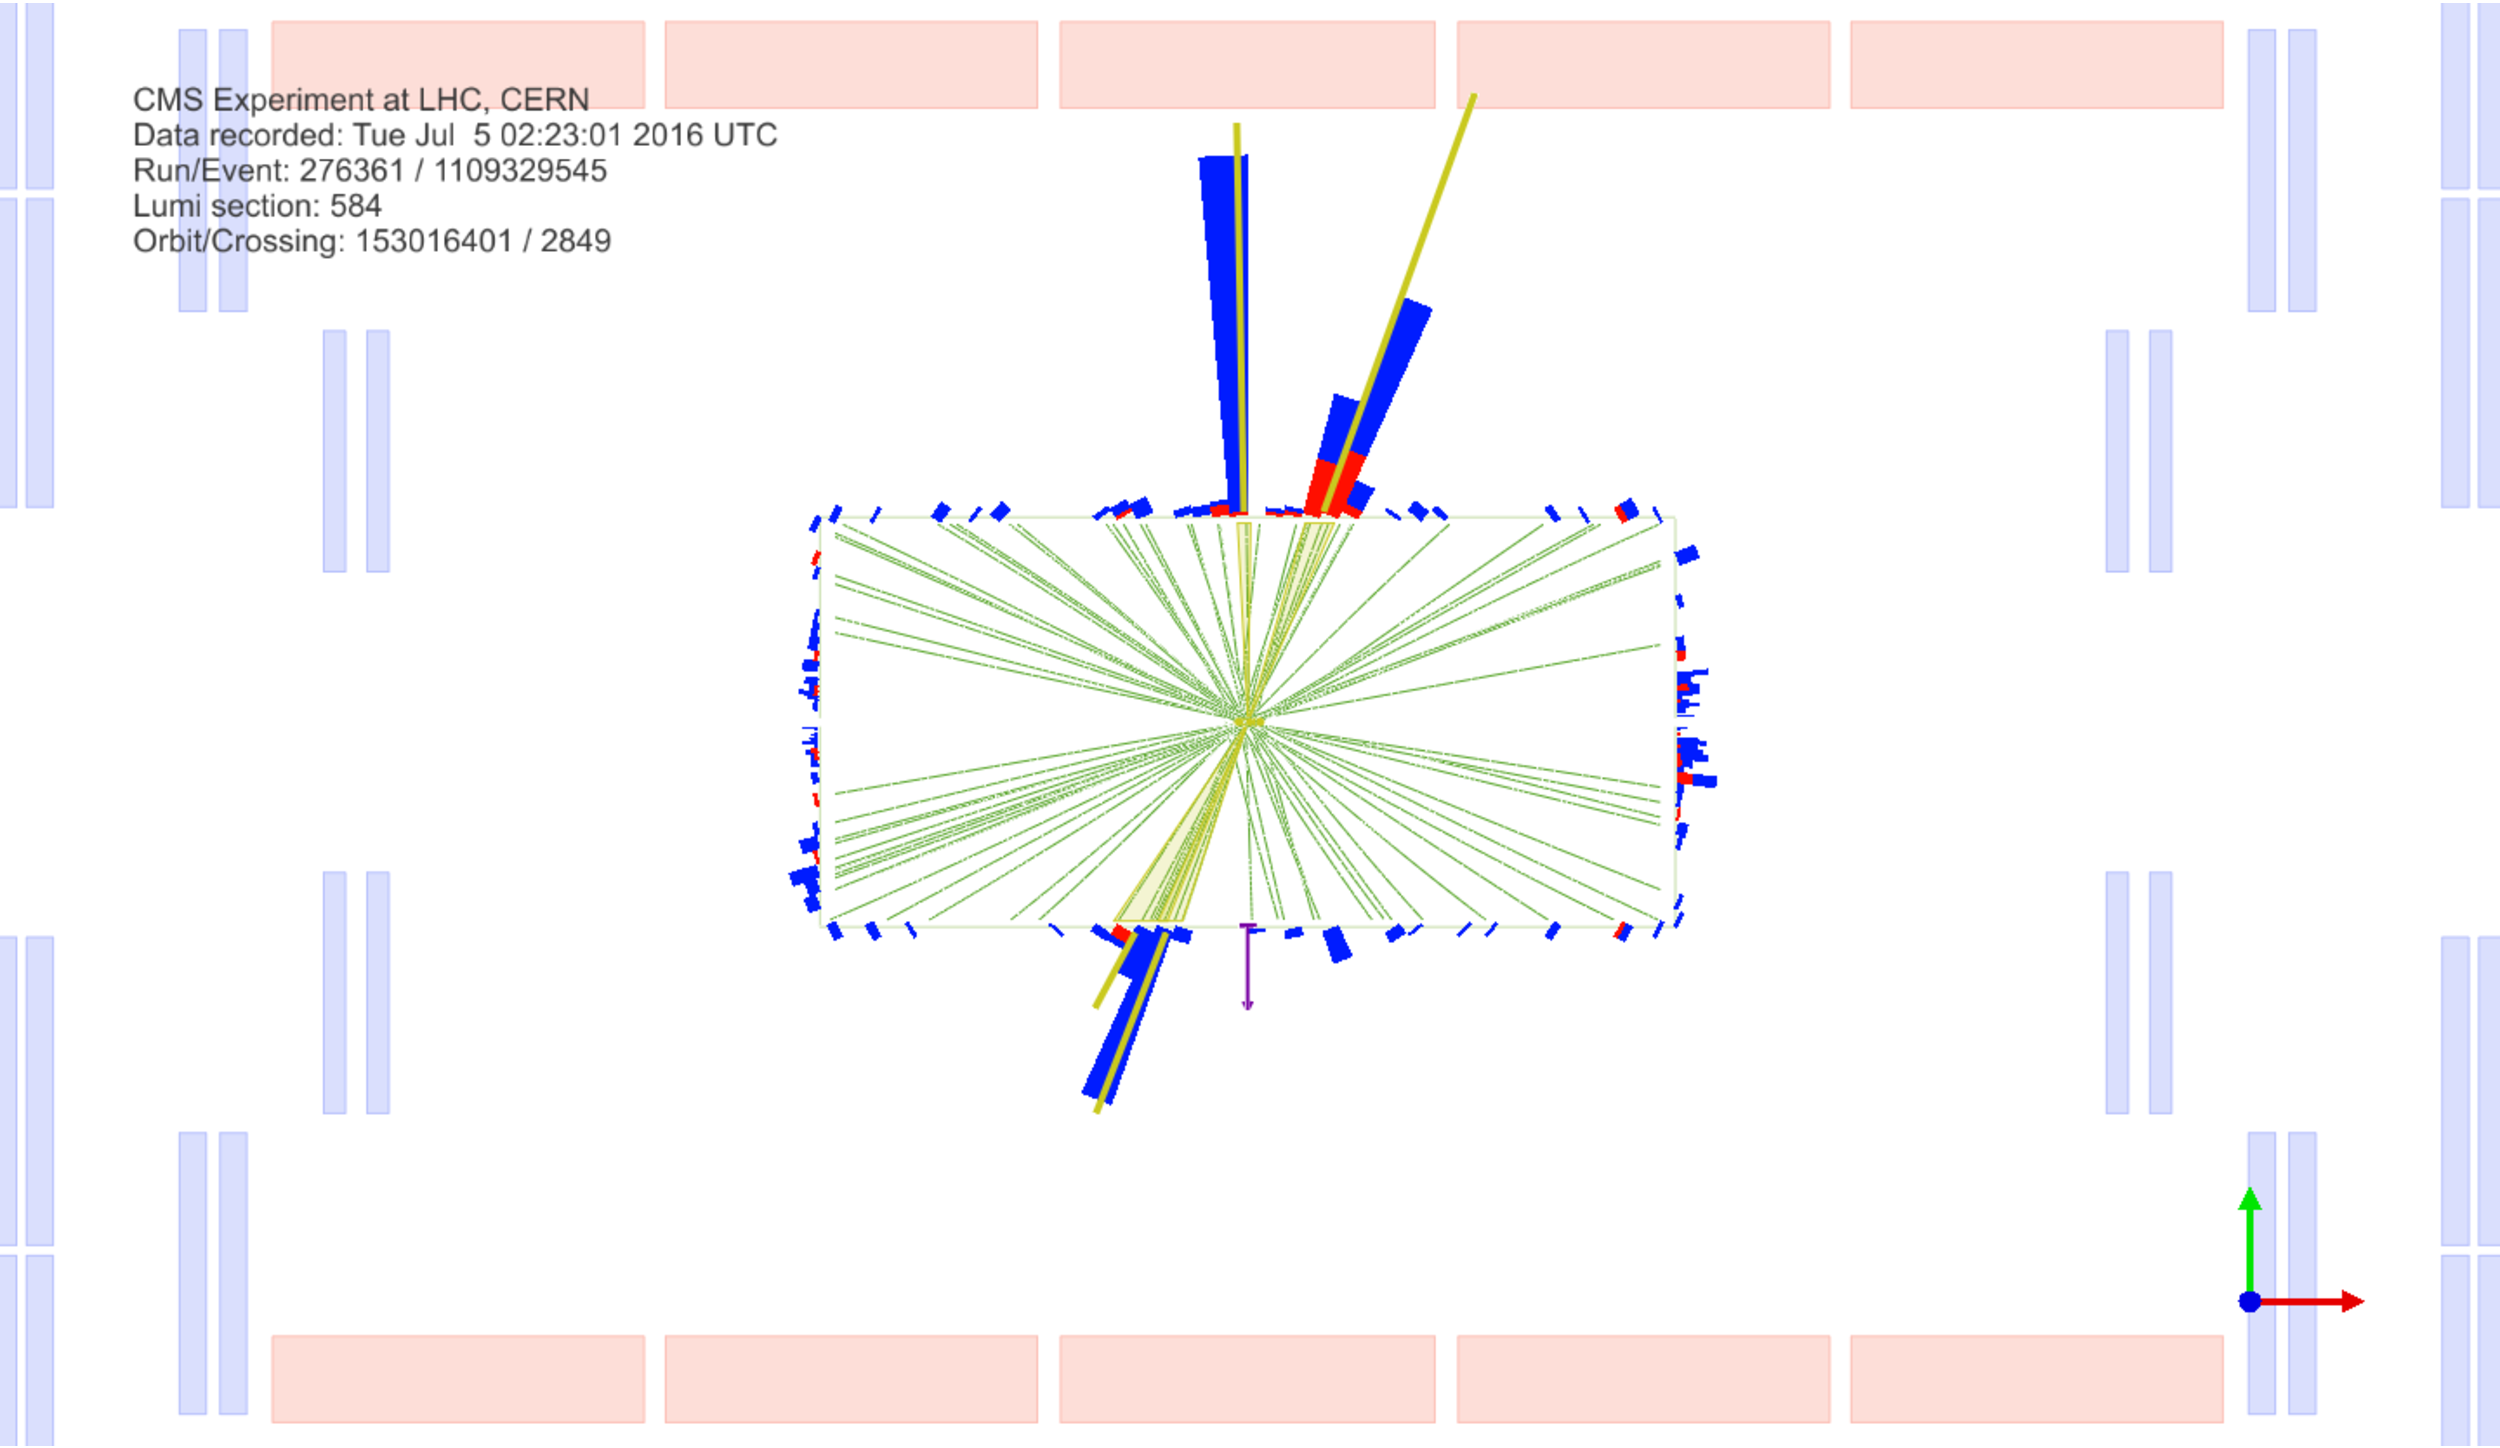
\includegraphics[width=.5\textwidth]{/home/bruno/org/PhD/Thesis/figures/intro/EvDisp_2016_tauTau_res2b_RhoZ.pdf}
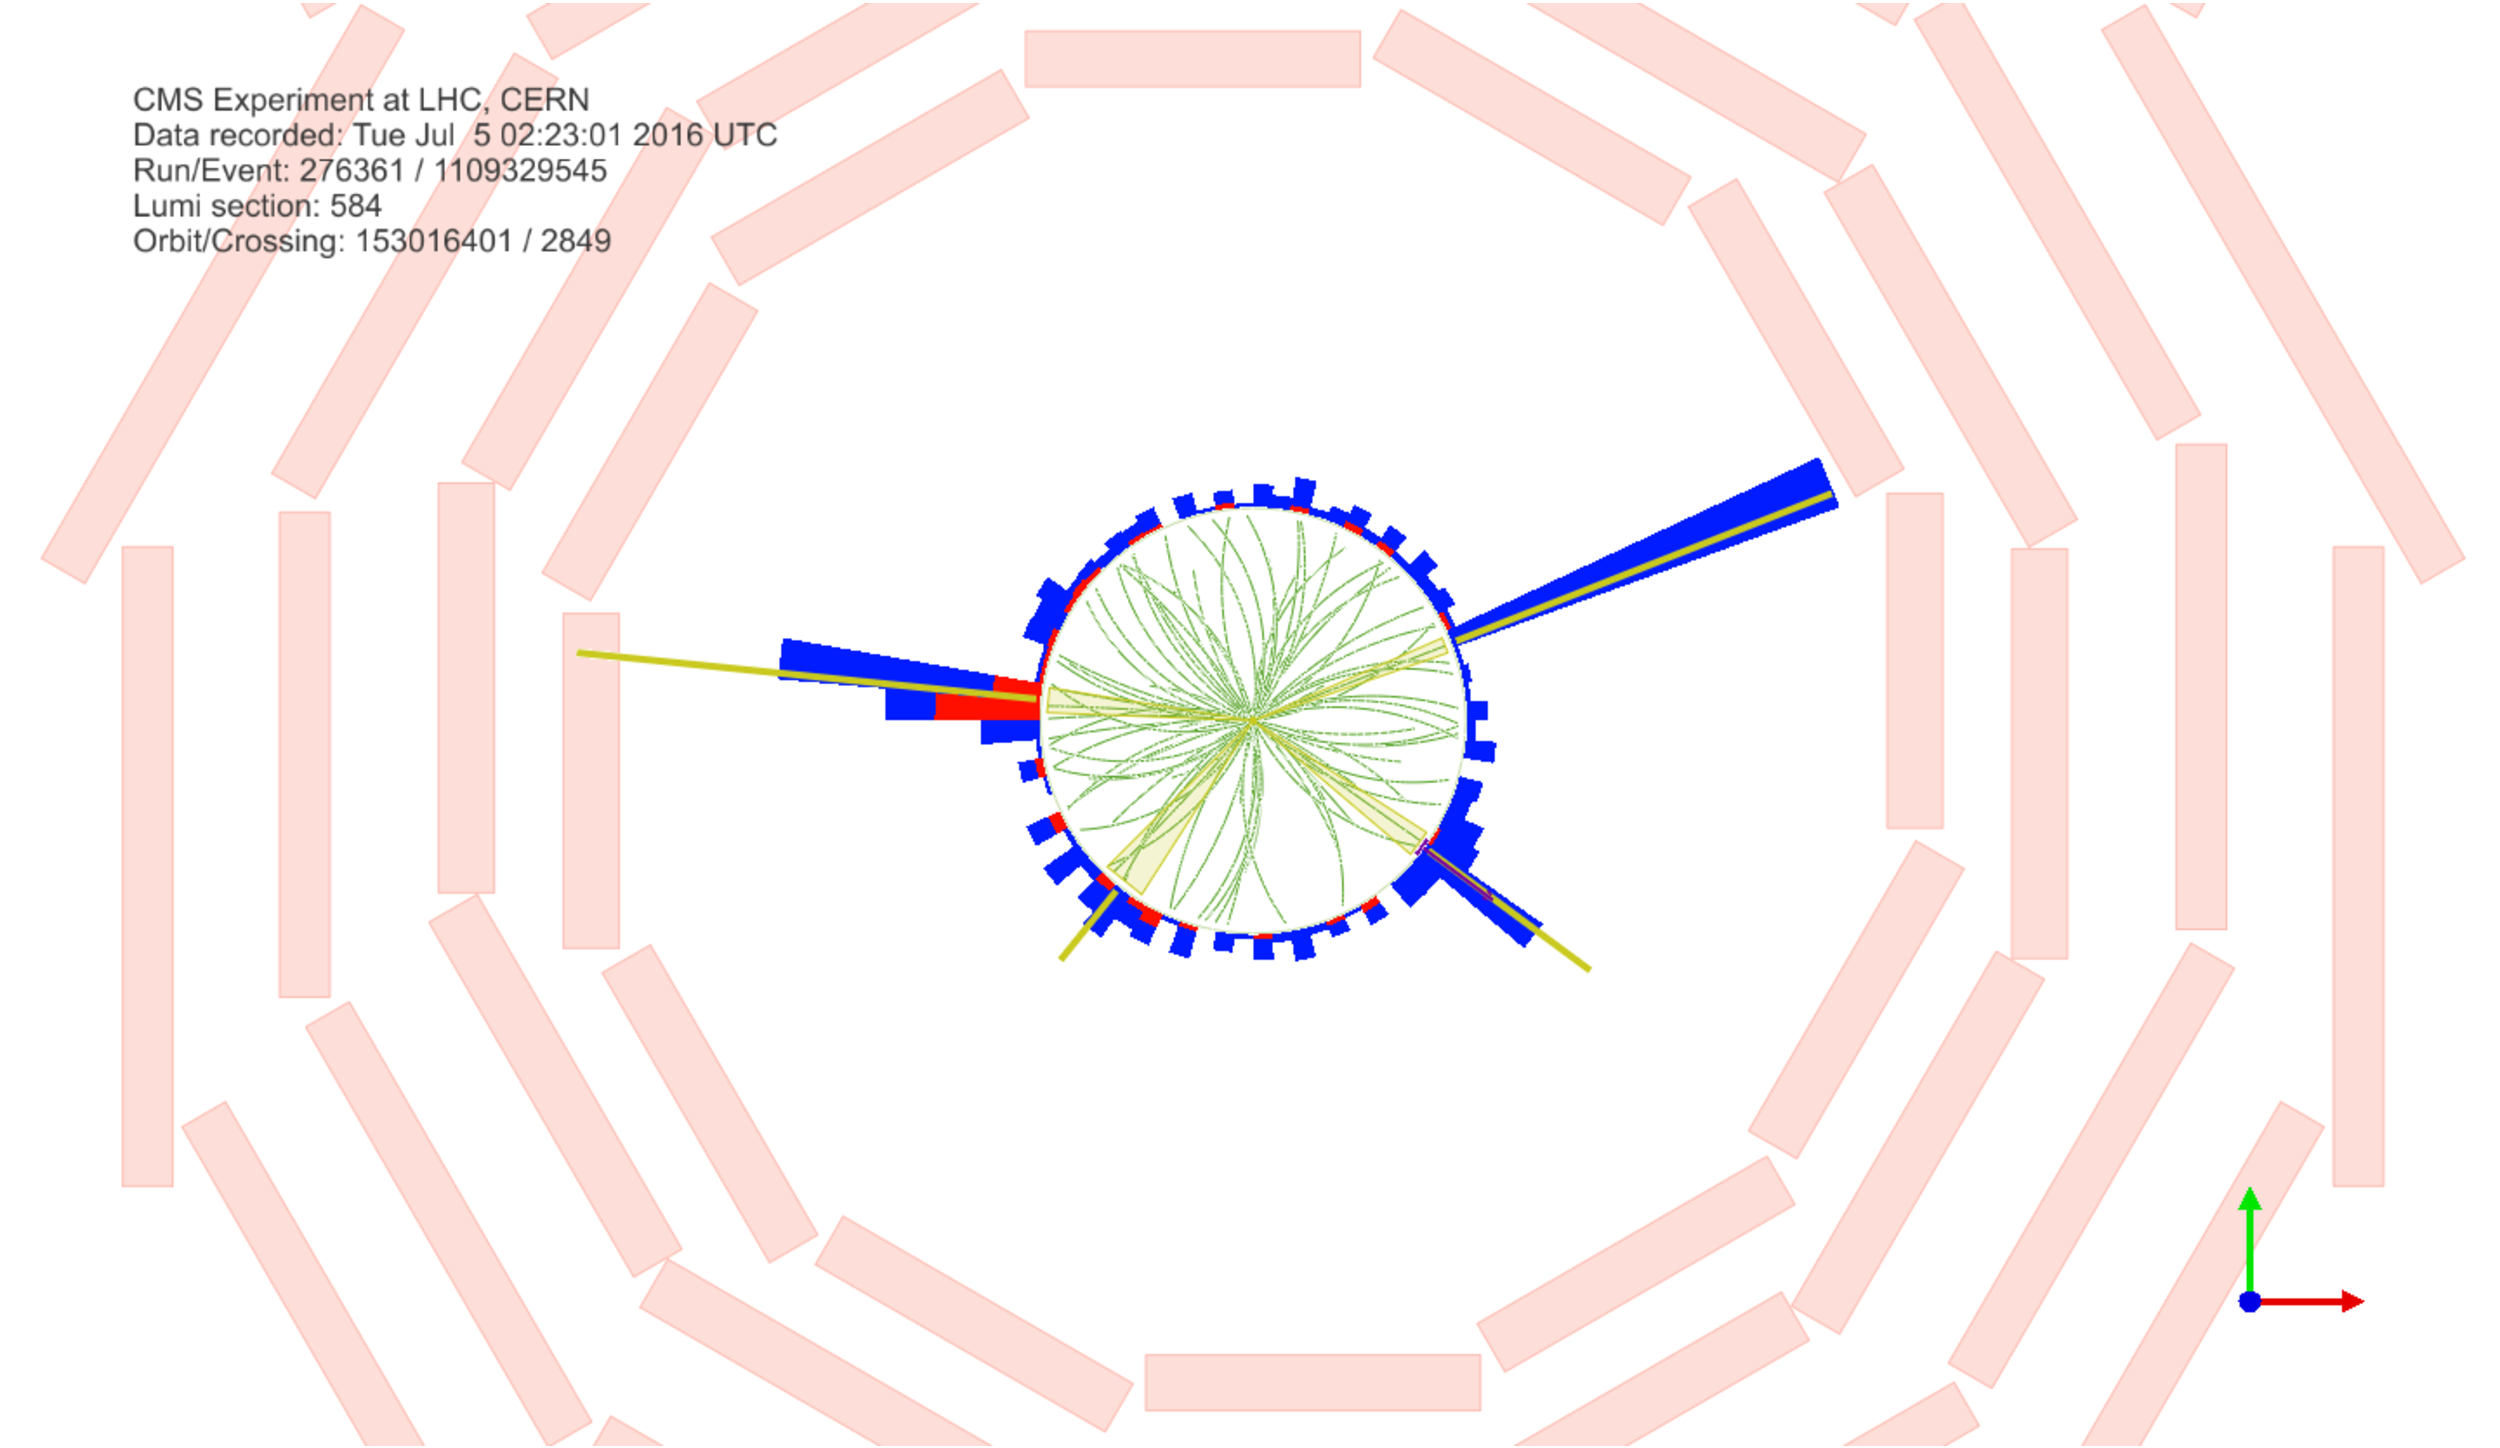
\includegraphics[width=.5\textwidth]{/home/bruno/org/PhD/Thesis/figures/intro/EvDisp_2016_tauTau_res2b_RhoPhi.pdf}
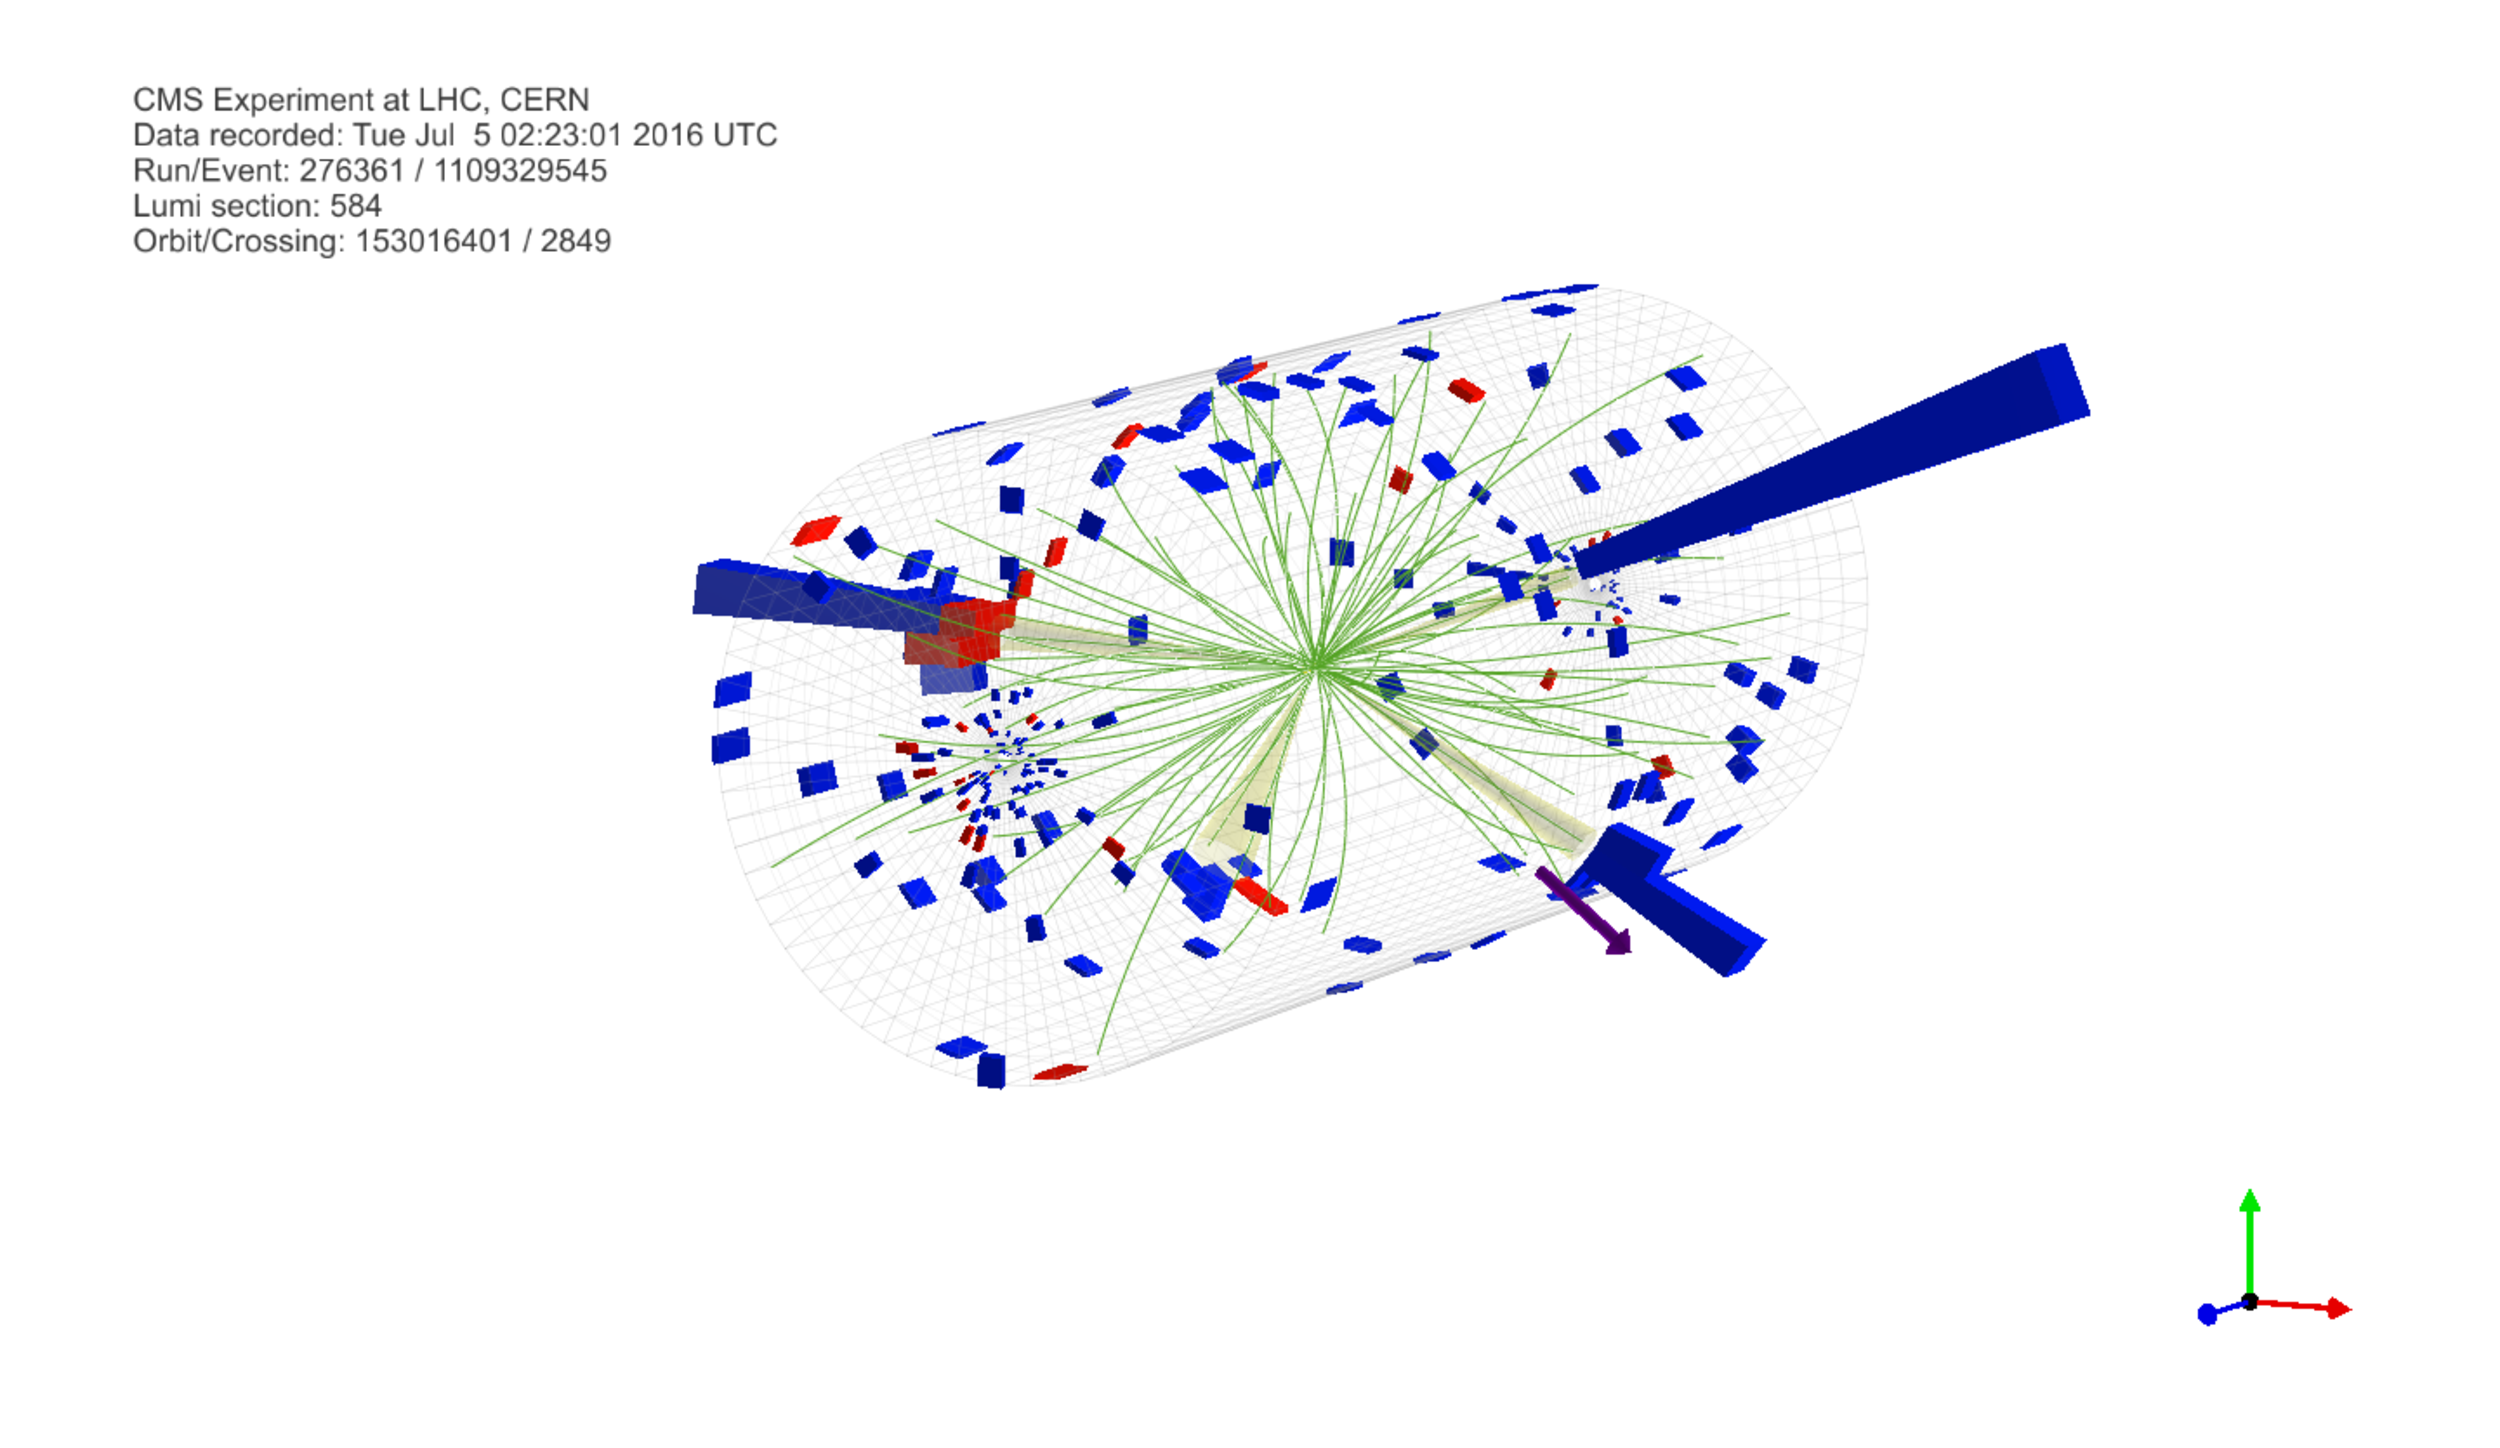
\includegraphics[width=1.\textwidth]{/home/bruno/org/PhD/Thesis/figures/intro/EvDisp_2016_tauTau_res2b_3D.pdf}
\caption{\label{fig:event_display_res2b_2016}\ac{CMS} event display for a \hhbbtt{} event in 2016. Three views are shown, namely \(R\) vs \(z\) (top left), \(R\) vs \(\phi\) (top right), and 3D in cartesian coordinates (bottom). Red and blue represent, respectively, \ac{ECAL} and \ac{HCAL} energy deposits, where the magnitude is proxied the dimension of each bar. Tracks are represented in green. The event passed the \rescat{2} selection. The selection of the analysis categories is defined in \cref{sec:categorization}.}
\end{figure}
\subsubsection{Production}
\label{sec:org0d501c1}
\label{sec:production}

The measurement of Higgs properties at the LHC are in general challenging, given the low cross-sections involved

gluon fusion is the dominant production mode.

\begin{figure}[htbp]
\centering
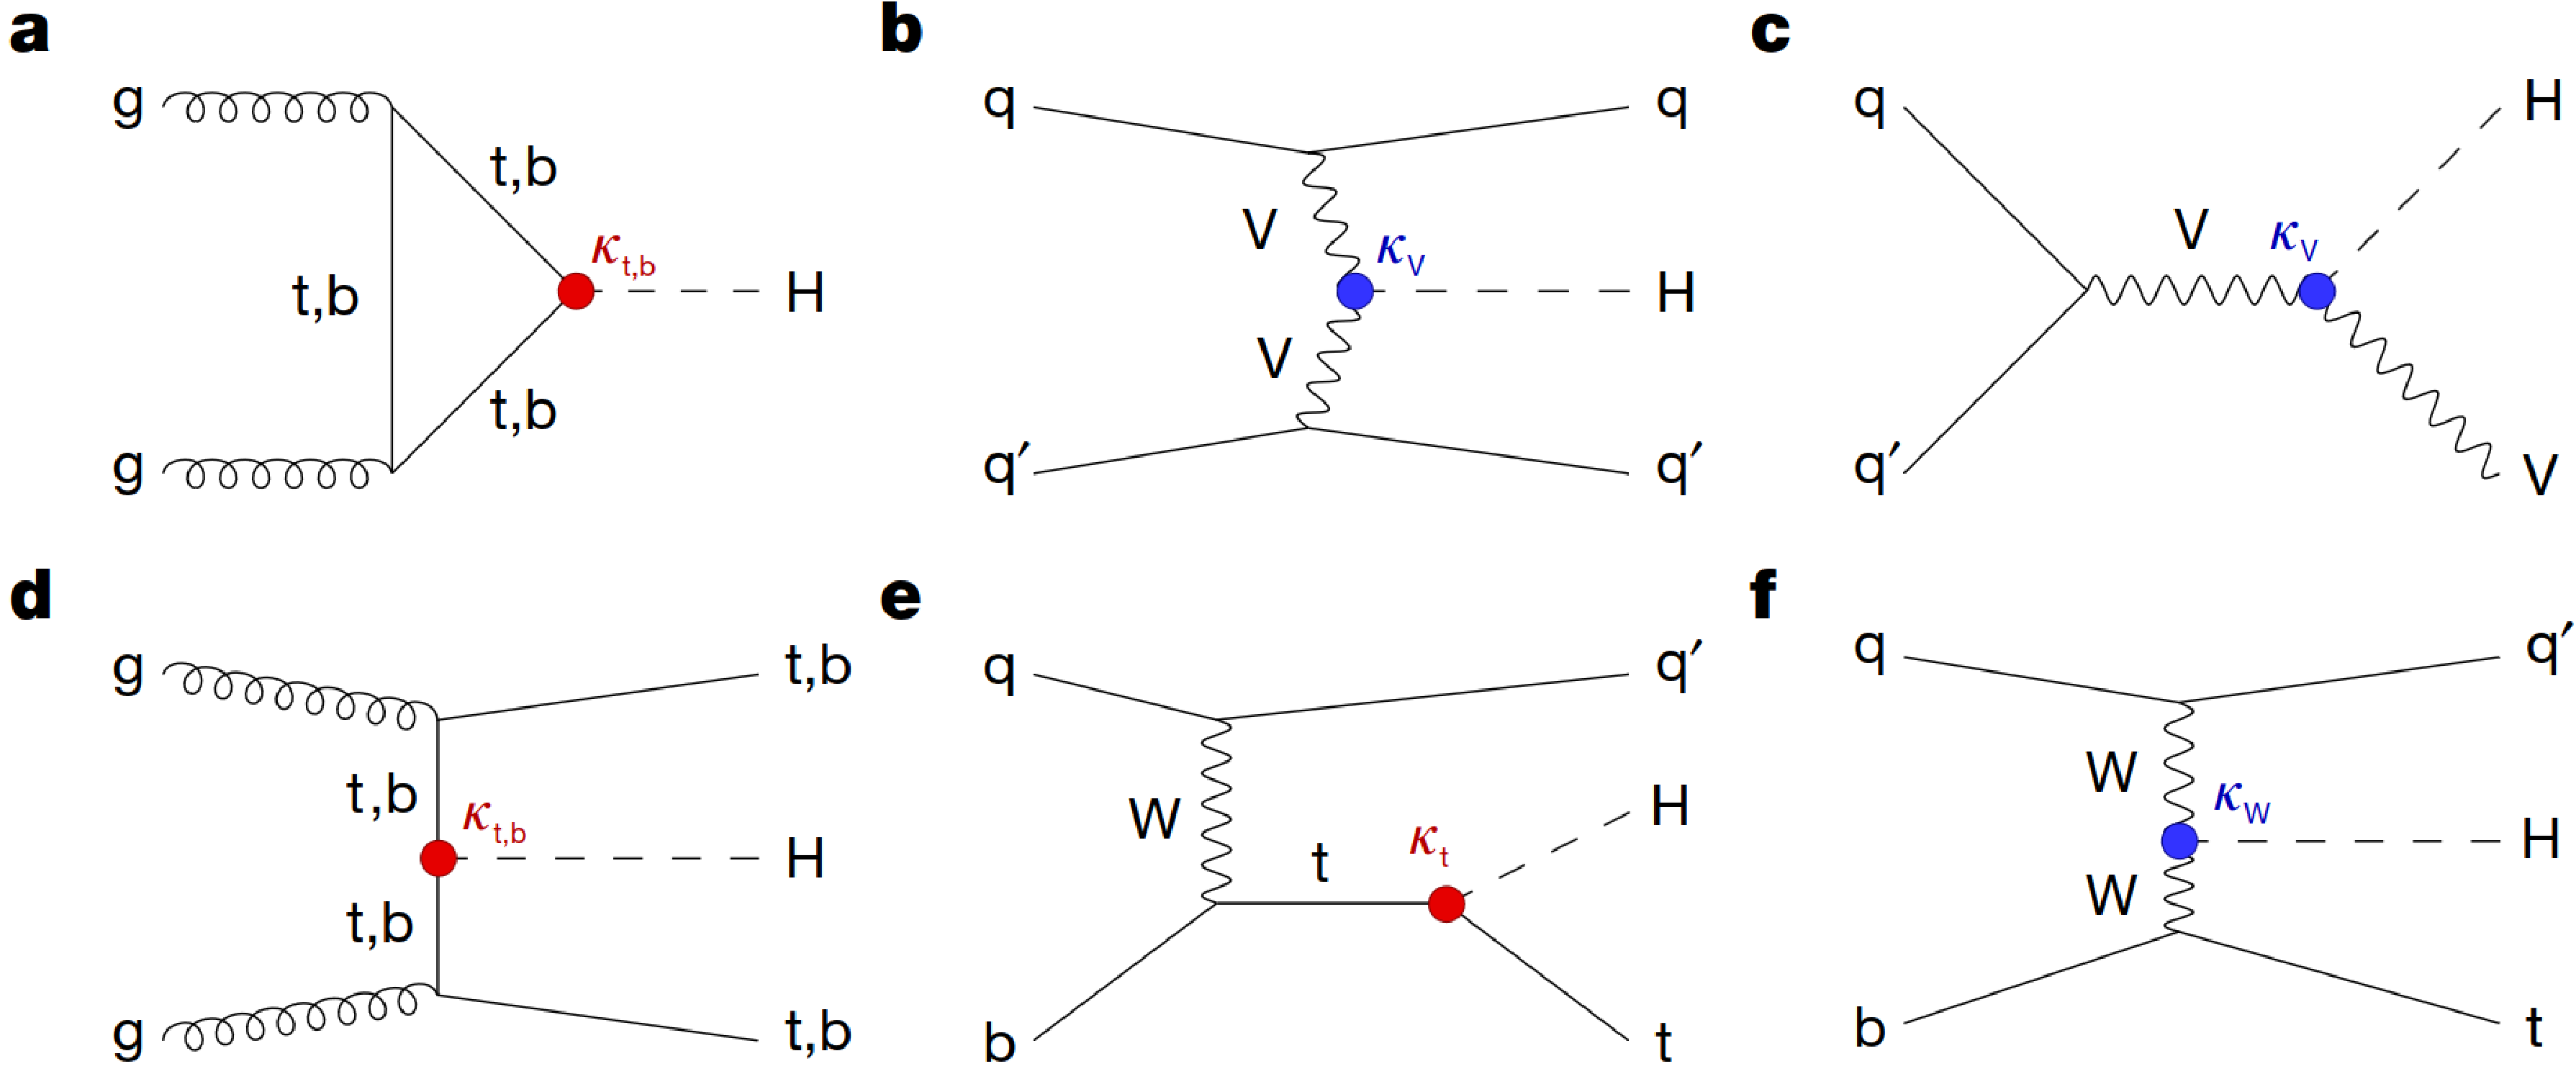
\includegraphics[width=.9\textwidth]{/home/bruno/org/PhD/Thesis/figures/intro/H_production_diagrams.pdf}
\caption{\label{fig:H_production_diagrams}Feynman diagrams for the leading Higgs boson production processes. \emph{a)} gluon fusion \emph{b)} \ac{VBF} \emph{c)} associated production with a W or Z (V) boson \emph{d)} associated production with a top or bottom quark pair \emph{e)} associated production with a single top quark. Taken from \cite{higgs_10_years}.}
\end{figure}

\begin{figure}[htbp]
\centering
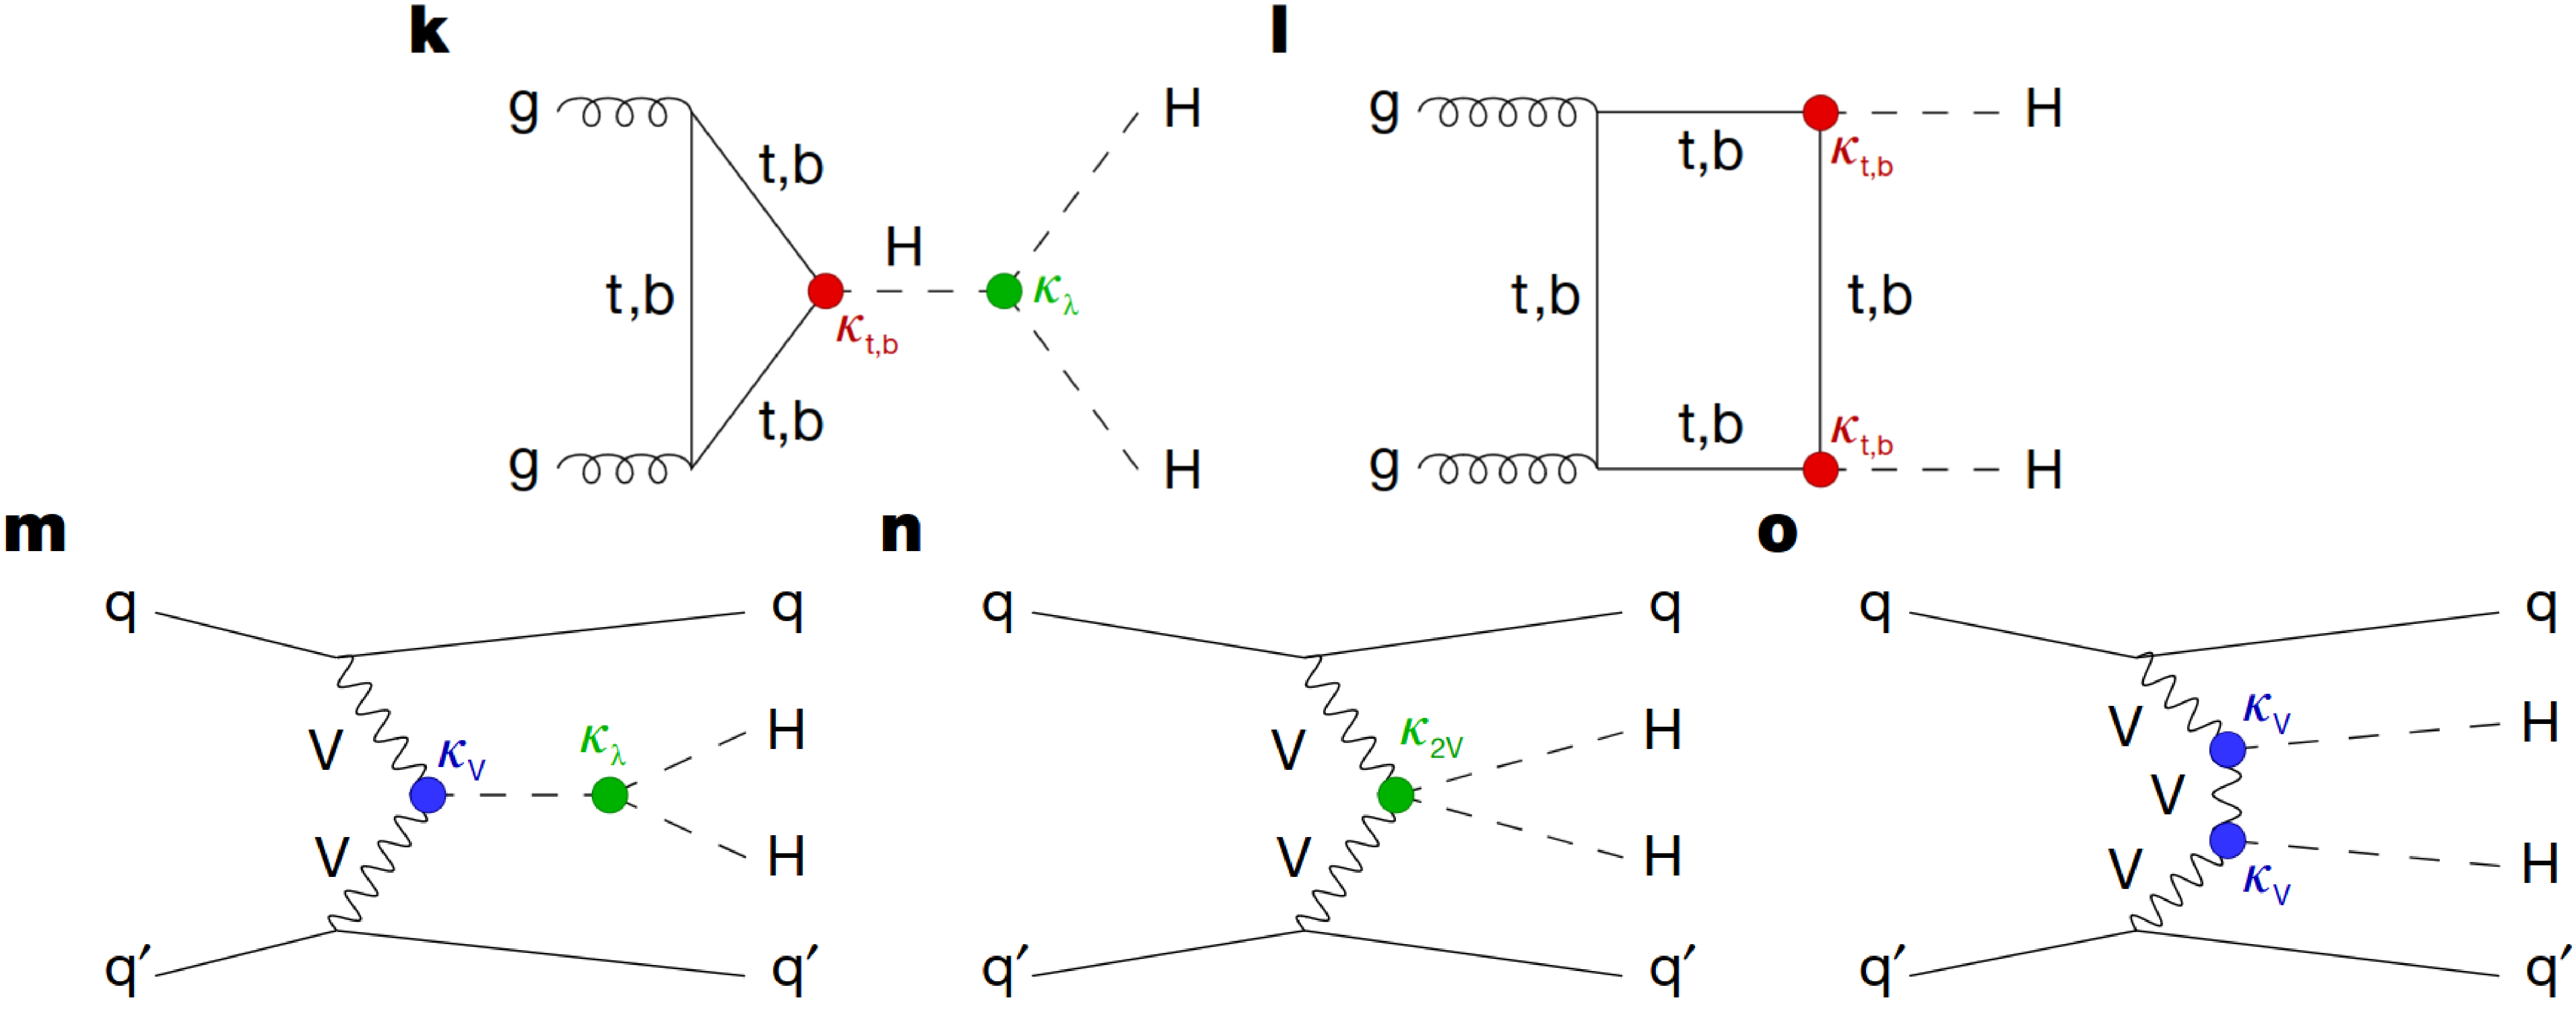
\includegraphics[width=.9\textwidth]{/home/bruno/org/PhD/Thesis/figures/intro/HH_production_diagrams.pdf}
\caption{\label{fig:HH_production_diagrams_b}Feynman diagrams for the leading H boson decay channels into: \emph{g)} heavy vector boson pairs \emph{h)} fermion anti-fermion pairs \emph{i)} photon pairs \emph{j)} Z\(\gamma\). Taken from \cite{higgs_10_years}.}
\end{figure}

\begin{figure}[htbp]
\centering
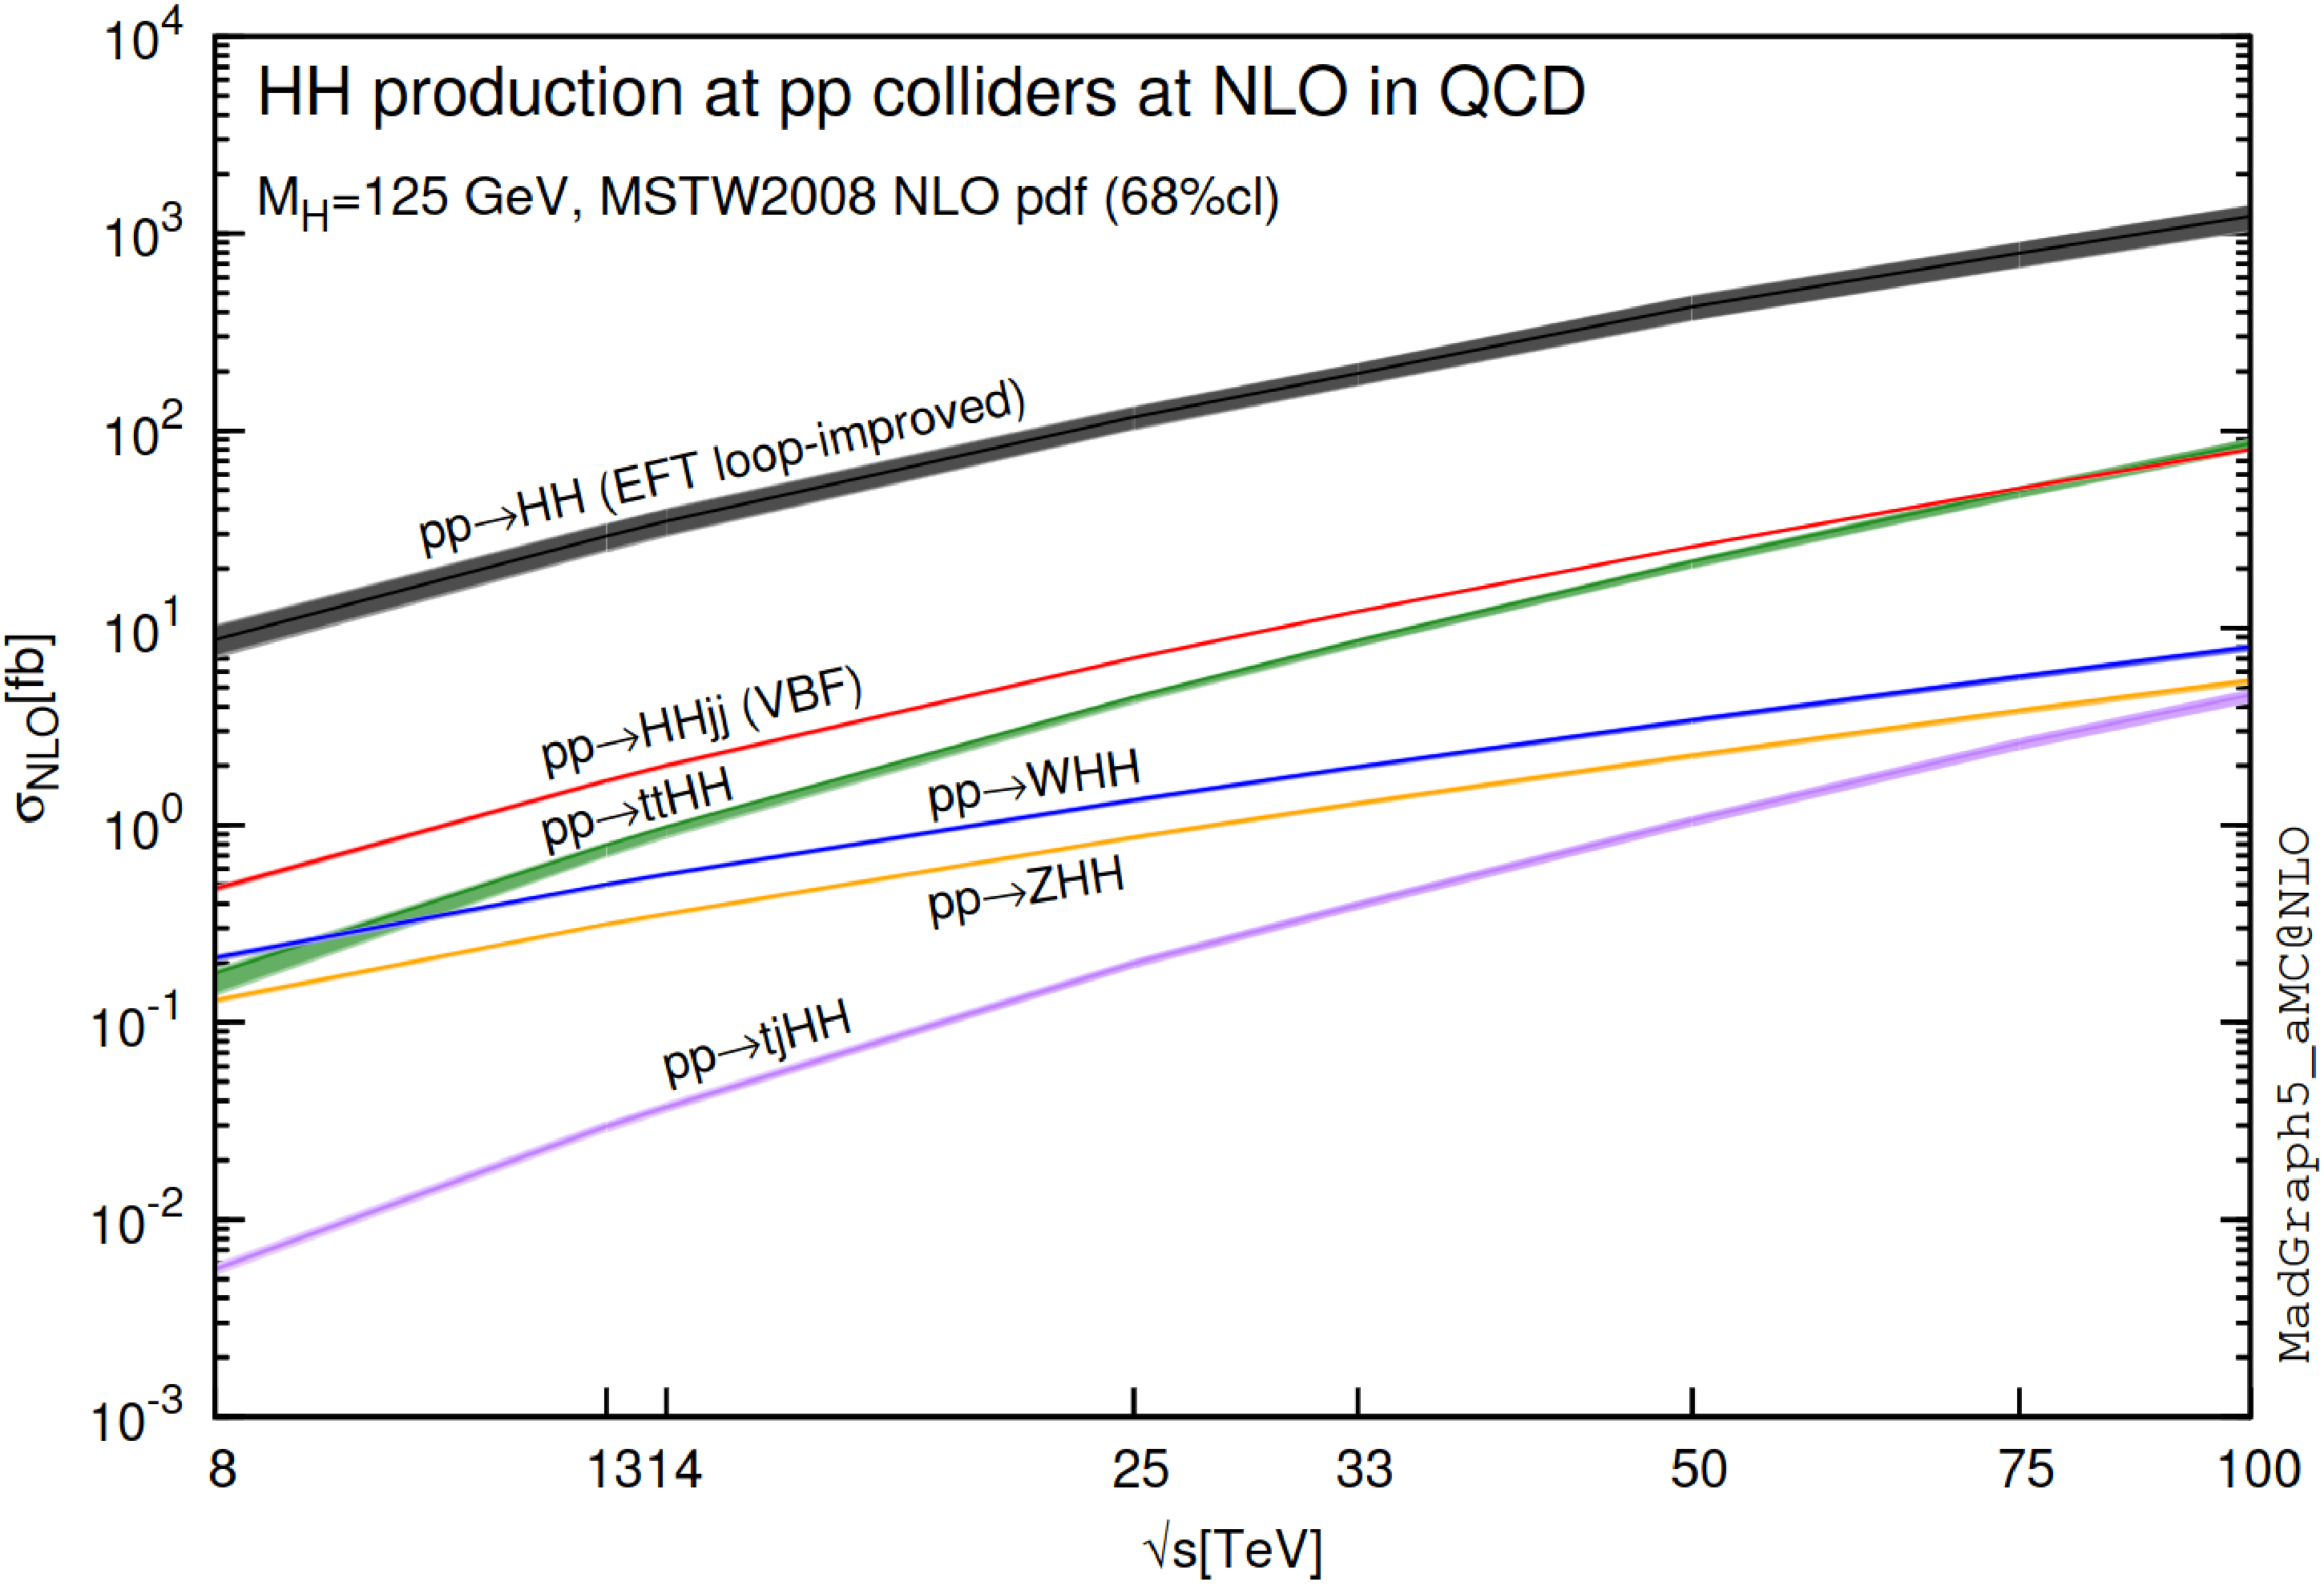
\includegraphics[width=.9\textwidth]{/home/bruno/org/PhD/Thesis/figures/intro/HH_production_energy.pdf}
\caption{\label{fig:HH_prod_energy}HH production cross section as a function of the center of mass energy for the six largest HH production channels at \emph{pp} colliders. The thickness of the lines corresponds to the scale and PDF uncertainties added linearly. Gluon fusion dominates for the entire energy range. The figure is taken from \cite{HH_xsec_running}.}
\end{figure}

\begin{figure}[htbp]
\centering
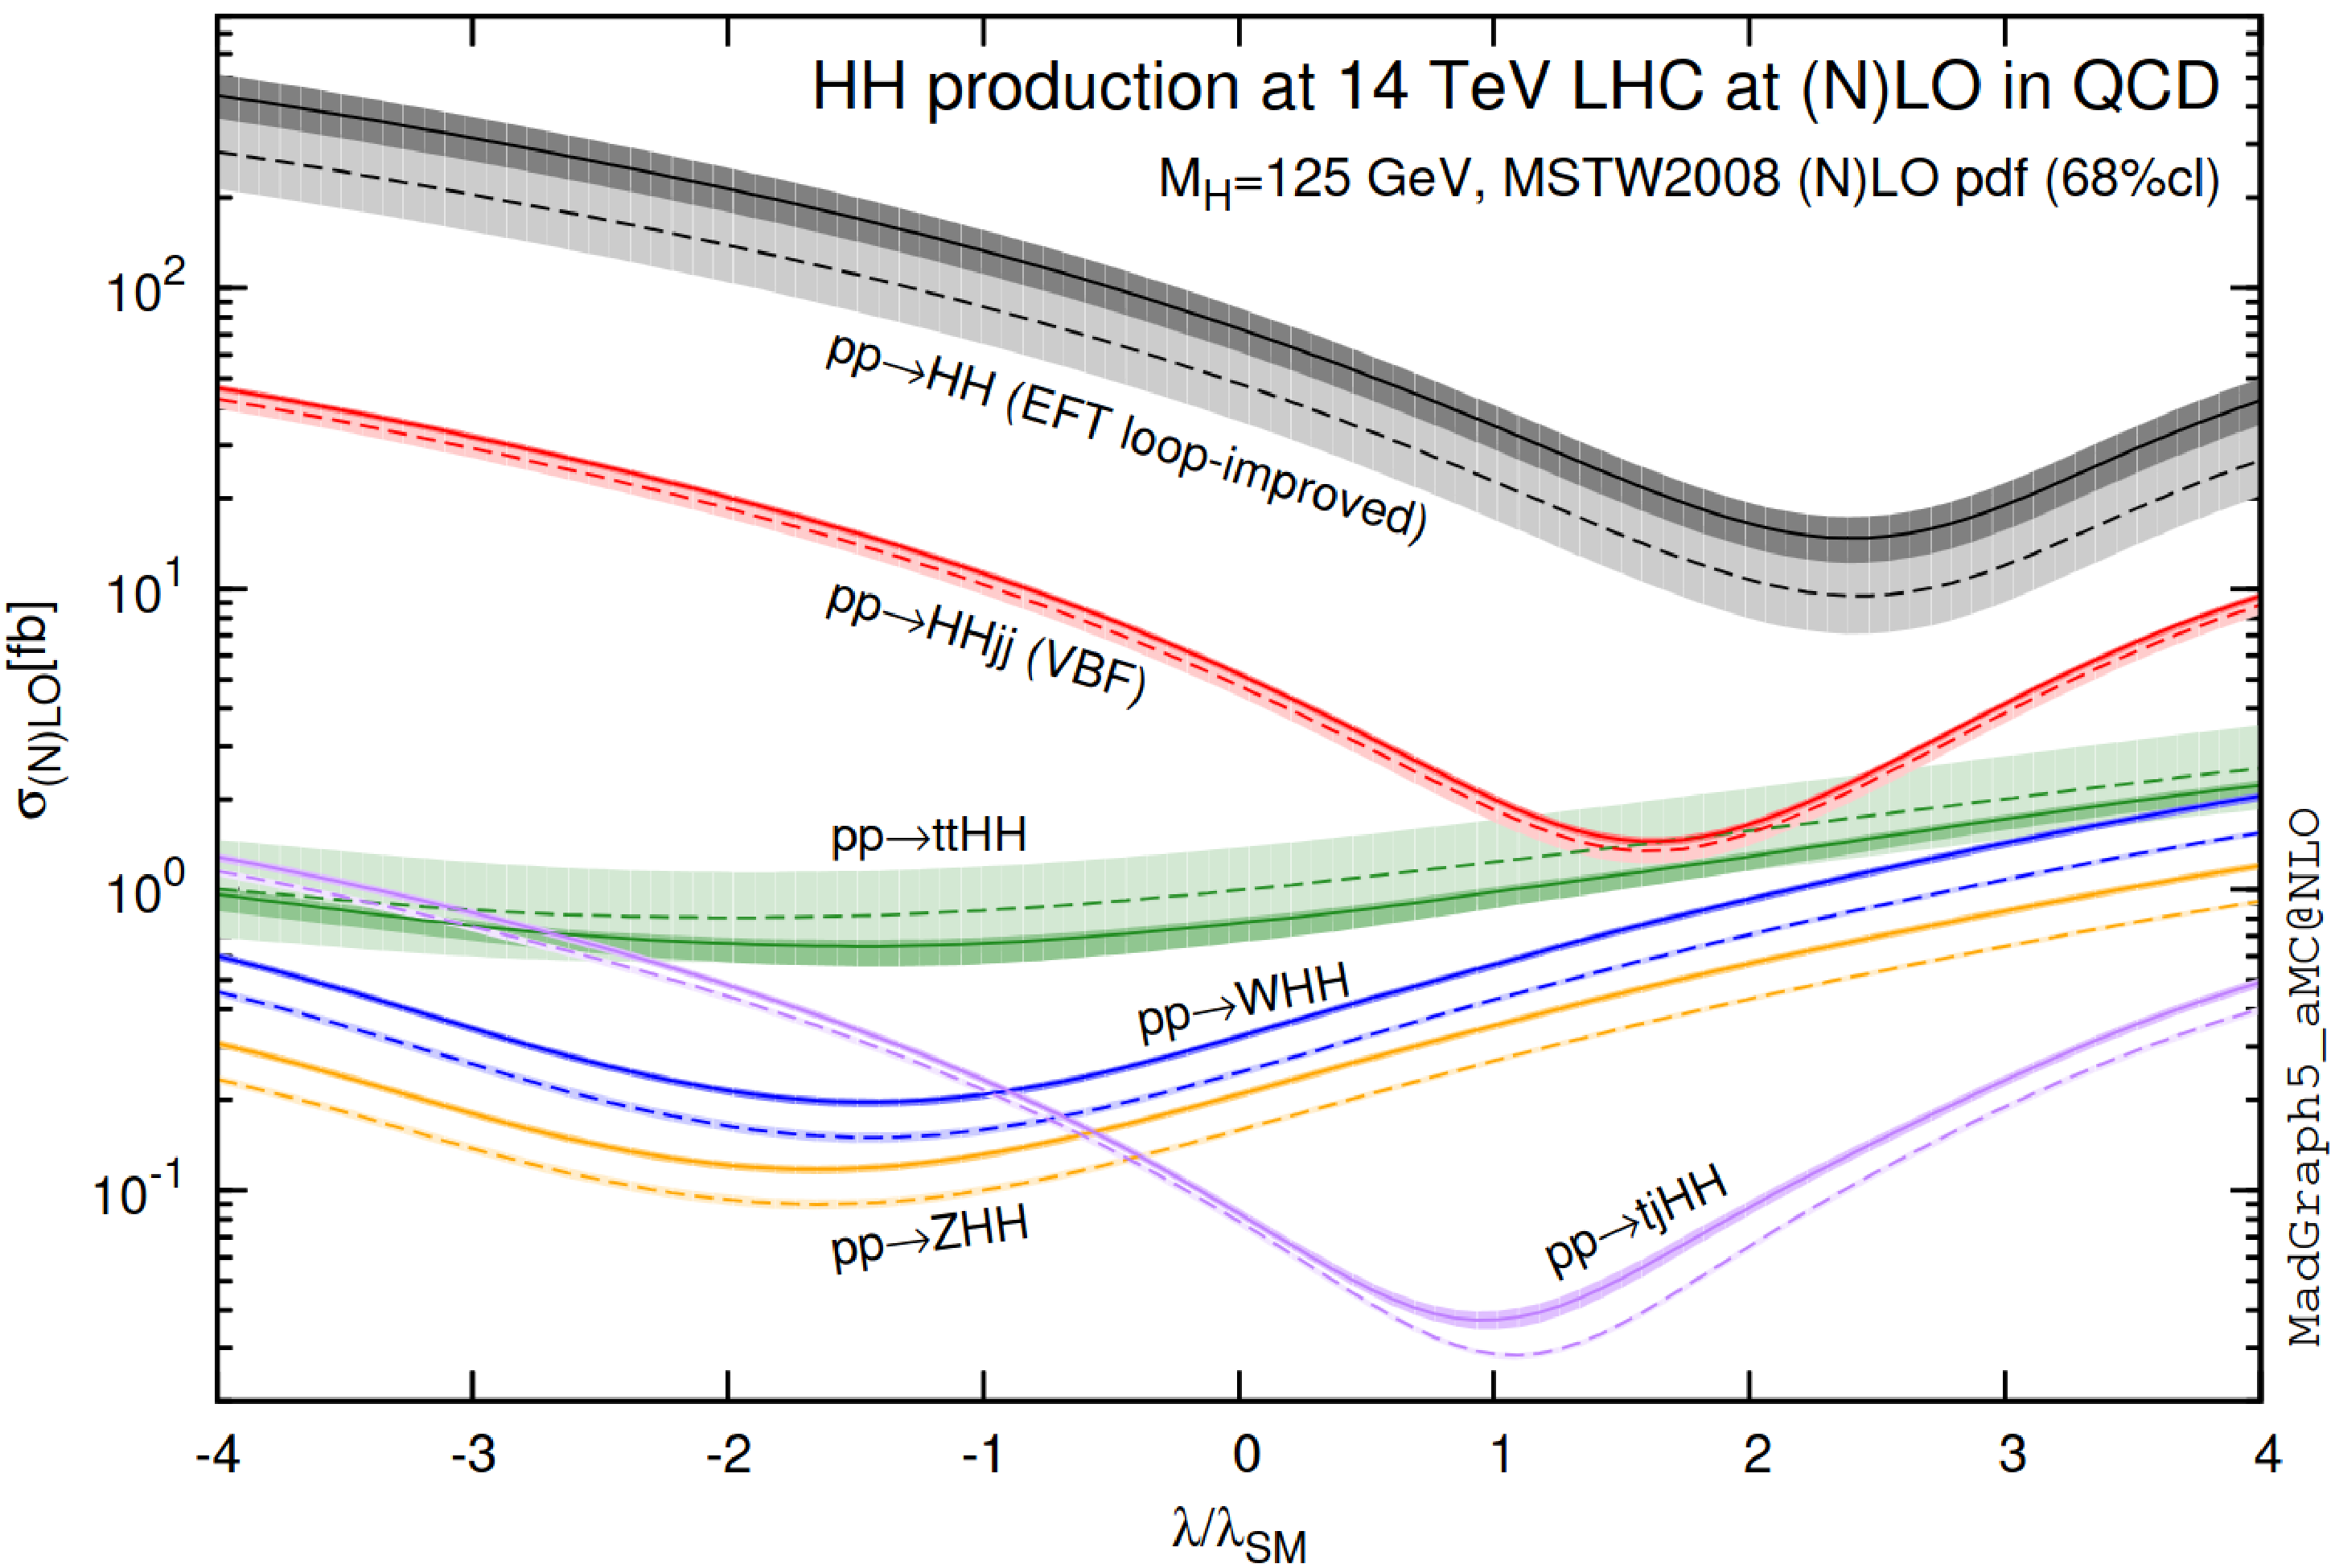
\includegraphics[width=.9\textwidth]{/home/bruno/org/PhD/Thesis/figures/intro/HH_production_kl.pdf}
\caption{\label{fig:HH_prod_kl}HH production cross section as a function of the coupling modifier \(\klrat\) for several production mechanisms. The dashed and solid lines denote respectively the LO and NLO predictions and the bands indicate the PDF and scale uncertainties added linearly. The figure is taken from \cite{HH_xsec_running}.}
\end{figure}

\begin{figure}[htbp]
\centering
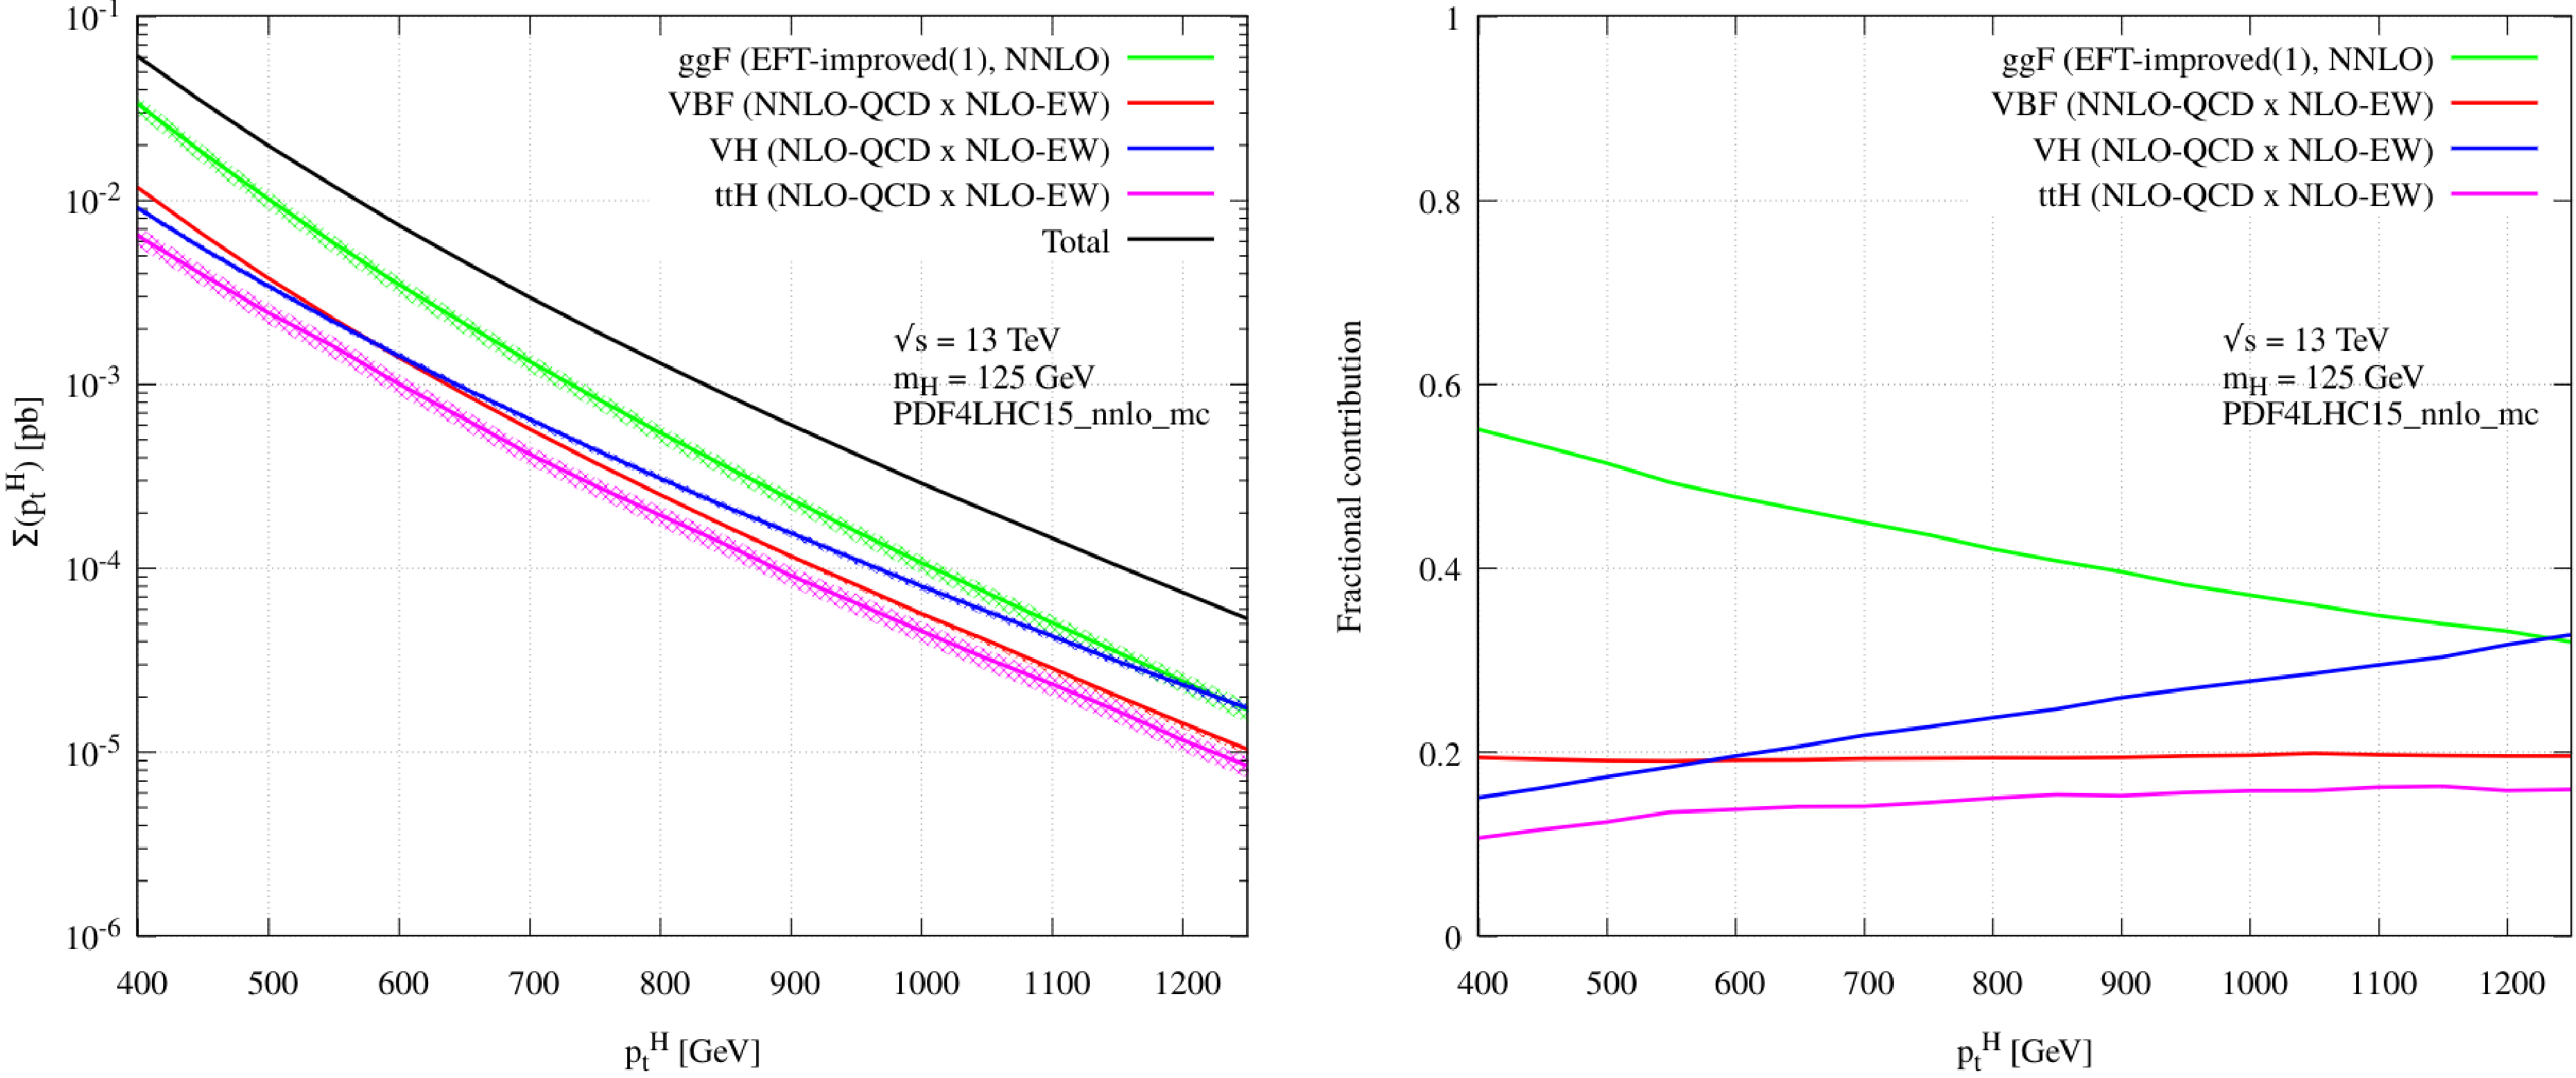
\includegraphics[width=.9\textwidth]{/home/bruno/org/PhD/Thesis/figures/intro/hh_xsec_evoluton_pt.pdf}
\caption{\label{fig:HH_prod_kl_b}Cumulative cross section for the production of a Higgs boson as a function of the lowest Higgs boson transverse momentum. The cross section due to \ac{ggF} (green), \ac{VBF} (red), vector boson associated (blue) and top-quark pair associated (magenta) production mode are shown in absolute values (left) and relative size (right). Taken from \cite{xsec_evolution_pt}.}
\end{figure}


\begin{table}[!h]
\centering
\begin{tabular}{c|c|c|c}
\(\sqrt{s}\) (\si{\TeV}) & \(\sigma^{\text{FTapprox}}_{\text{NNLO}}\) (\si{\femto\barn}) & PDF + \(\alpha_{S}\) unc. & Scale + \(m_{t}\) unc.\\
\hline
7 & 6.572 & \textpm{}4.3\% & \(-\)\\
8 & 9.441 & \textpm{}3.9\% & \(-\)\\
13 & 31.05 & \textpm{}3.0\% & \(-23\% +6\%\)\\
13.6 & 34.43 & \textpm{}3.0\% & \(-23\% +6\%\)\\
14 & 36.69 & \textpm{}3.0\% & \(-23\% +6\%\)\\
27 & 139.9 & \textpm{}2.5\% & \(-22\% +5\%\)\\
100 & 1224 & \textpm{}2.4\% & \(-21\% +4\%\)\\
\end{tabular}
\caption{\label{tab:HH_production_xsec}Inclusive gluon fusion cross-sections for HH production for different centre-of-mass energies in the \ac{NNLO} \ac{FT} approximation, for \(\mh=\SI{125}{\GeV}\), with the central scale set to \(\mhh/2\) (see \cite{higgs_xsec_top_effects}). PDF, \(\alpha_{S}\), scale and top mass \(m_{t}\) uncertainties are also showcased. Taken from \cite{lhc_wg4_twiki}.}

\end{table}
\subsubsection{Decay}
\label{sec:org46c88d6}
\label{sec:Decay}

\begin{figure}[htbp]
\centering
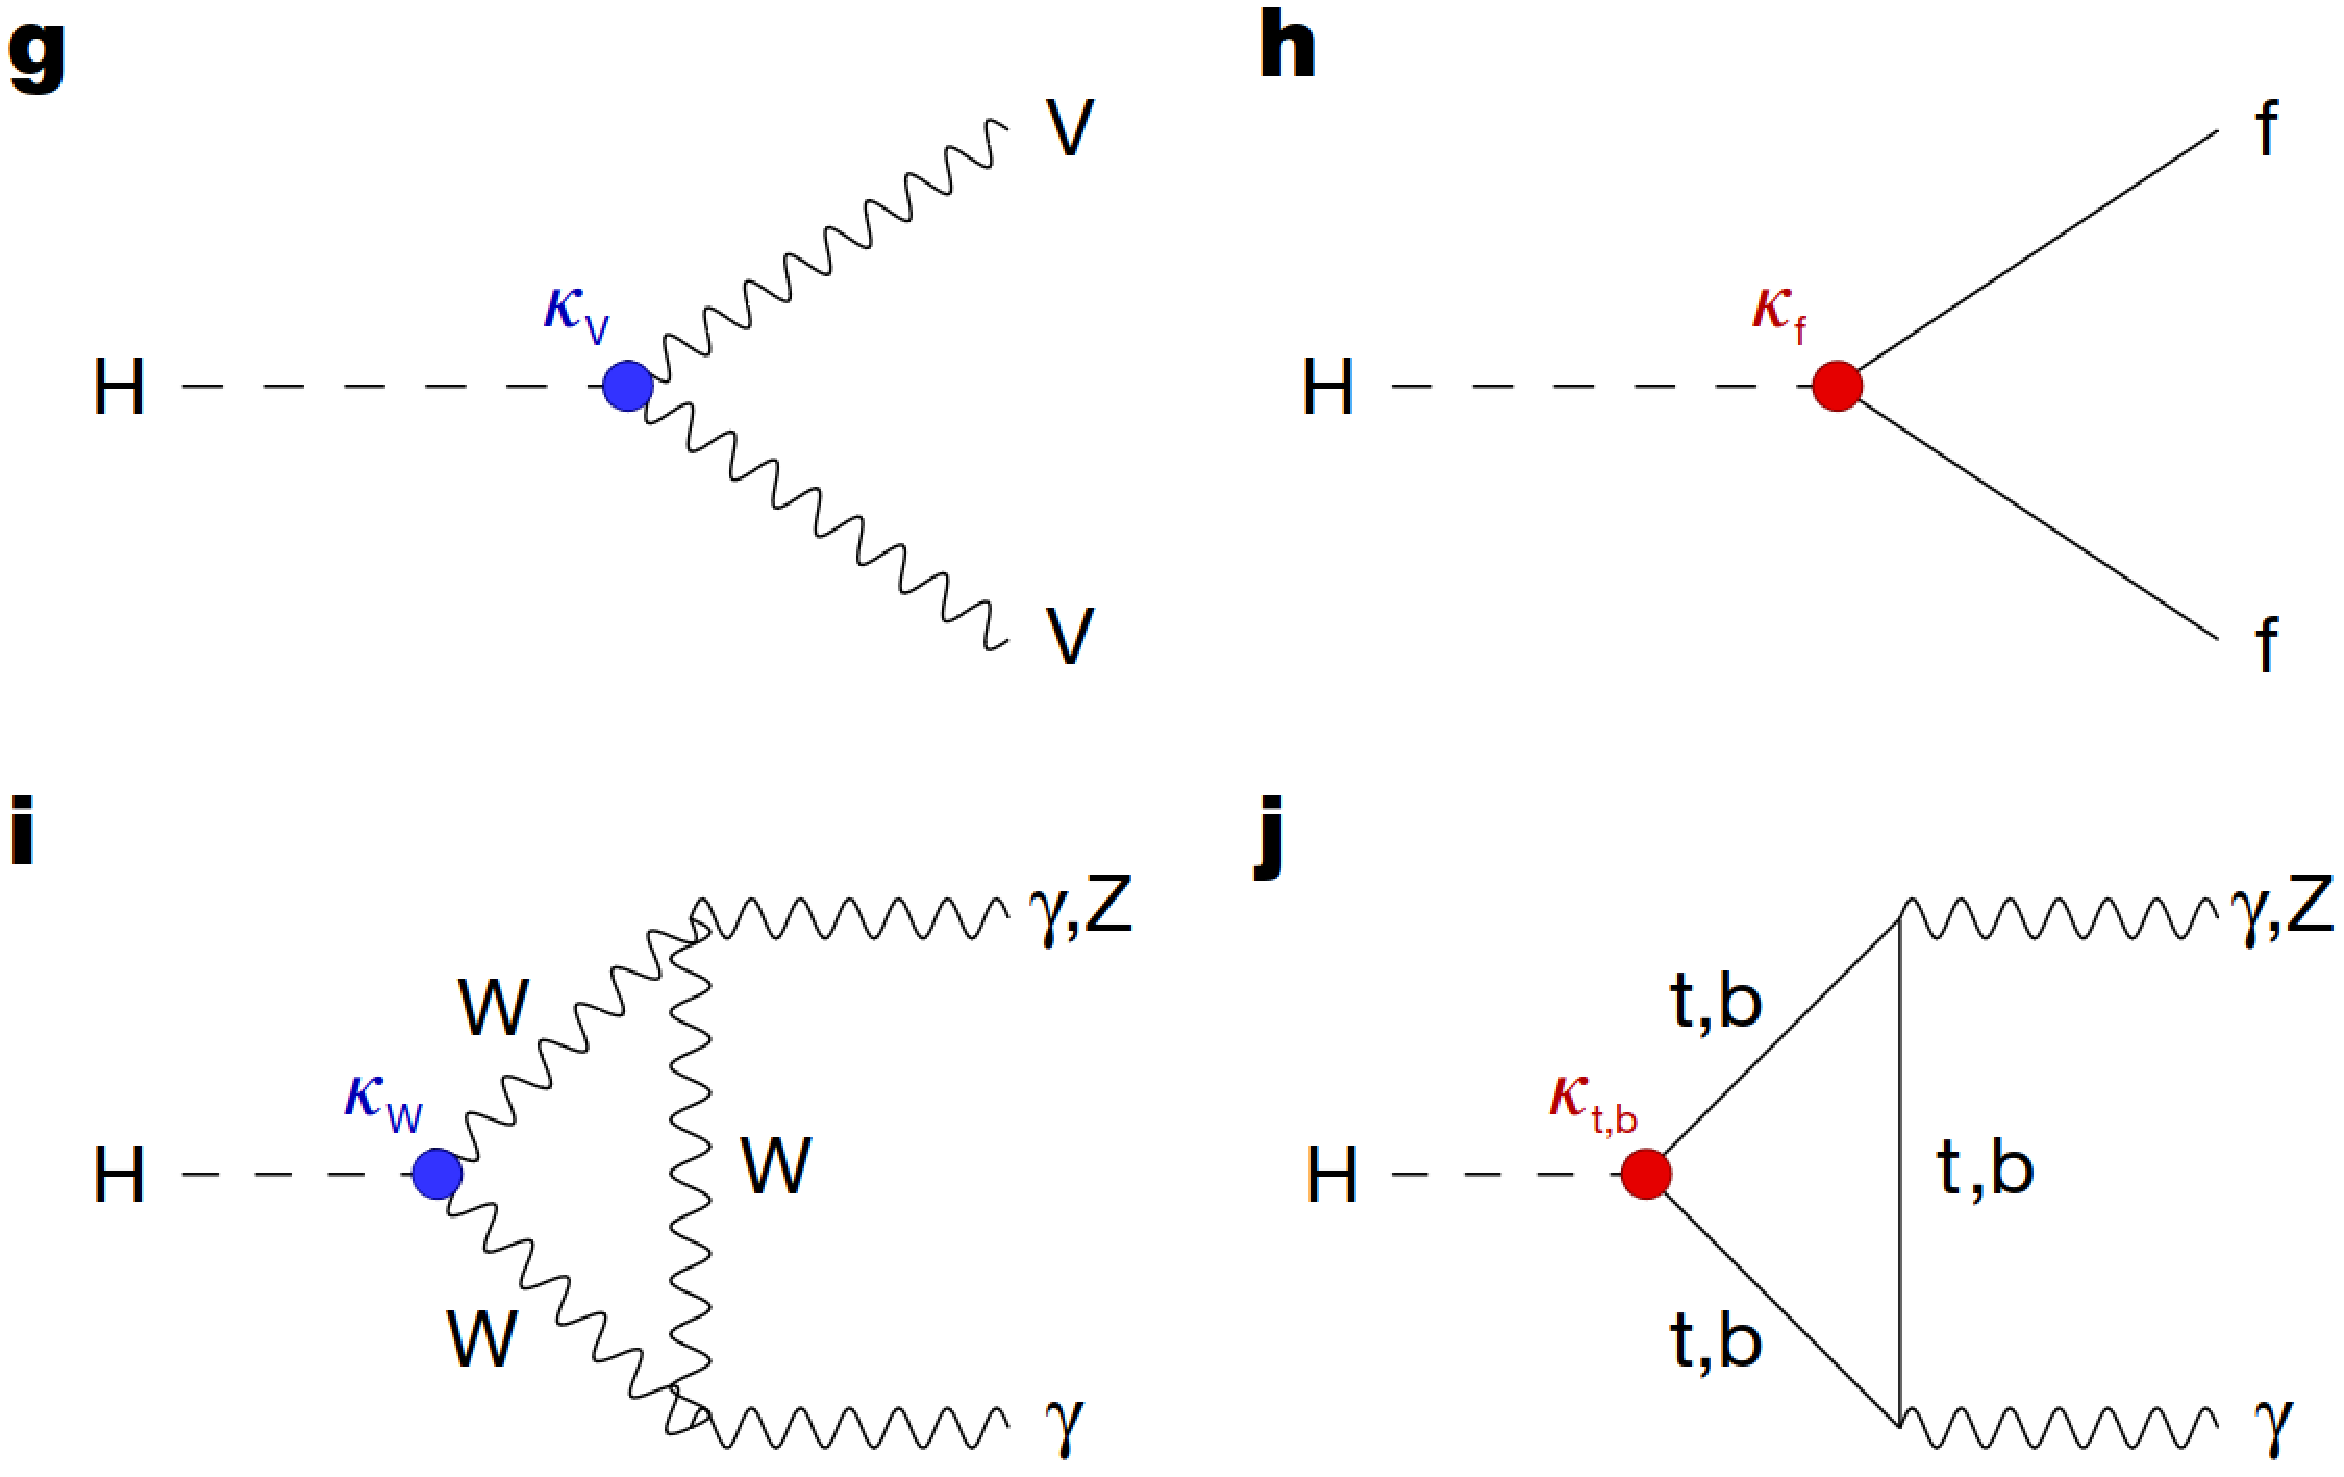
\includegraphics[width=.6\textwidth]{/home/bruno/org/PhD/Thesis/figures/intro/H_decay_diagrams.pdf}
\caption{\label{fig:HH_decay_diagrams}Feynman diagrams for the leading Higgs boson decay channels into: \emph{g)} heavy vector boson pairs \emph{h)} fermion anti-fermion pairs \emph{i)} photon pairs \emph{j)} \(Z\gamma\). Taken from \cite{higgs_10_years}.}
\end{figure}

\begin{figure}[htbp]
\centering
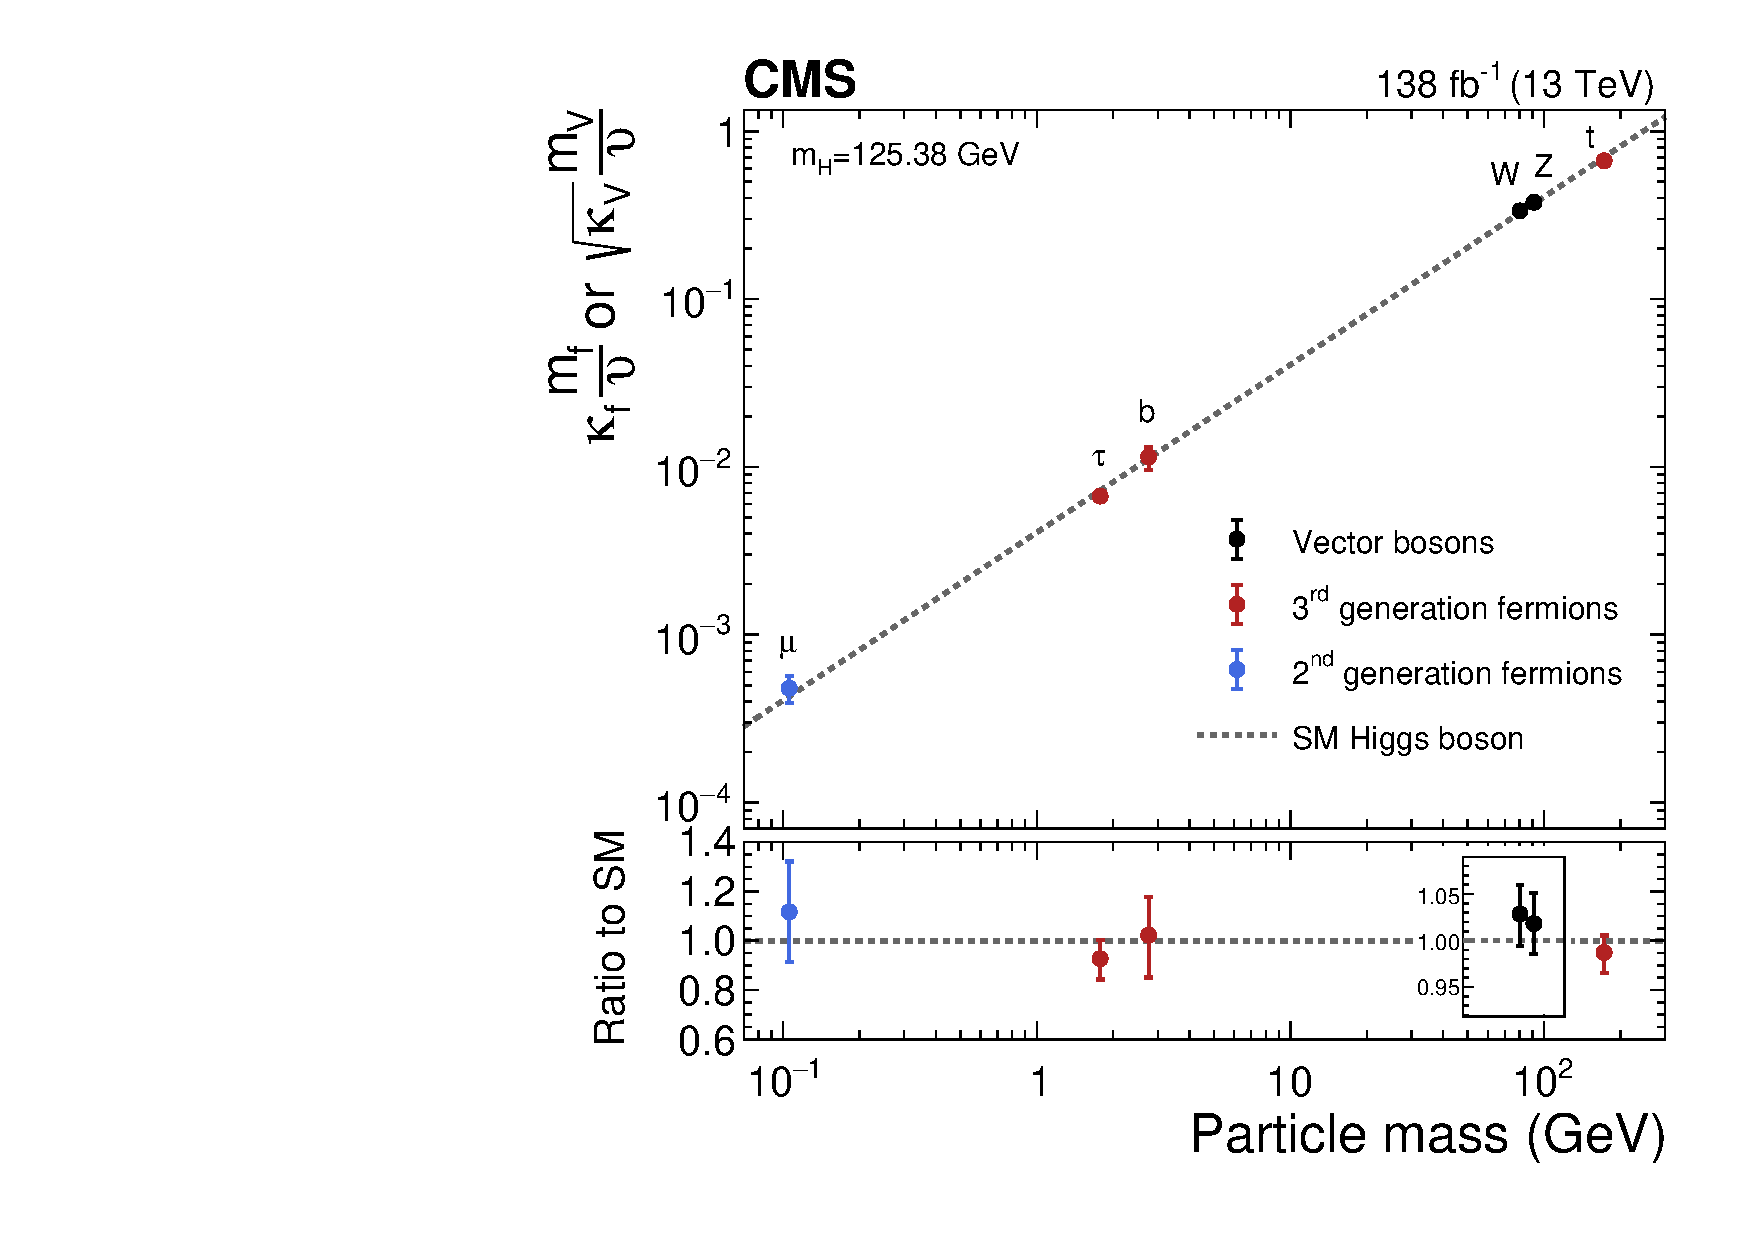
\includegraphics[width=.6\textwidth]{/home/bruno/org/PhD/Thesis/figures/intro/higgs_couplings_line.pdf}
\caption{\label{fig:HH_coupling_modifiers}The measured coupling modifiers of the Higgs boson to fermions and heavy gauge bosons, as functions of fermion or gauge boson mass, where υ is the vacuum expectation value of the Higgs field. For gauge bosons, the square root of the coupling modifier is plotted, to keep a linear proportionality to the mass, as predicted in the \ac{SM}. The p-value with respect to the SM prediction is 37.5\%. Taken from \cite{higgs_10_years}.}
\end{figure}
\begin{enumerate}
\item The bb\(\tau \tau\) final state
\label{sec:orge557fbb}

\item Other final states
\label{sec:orgea238d4}
\end{enumerate}
\subsection{Experimental status of SM HH Physics}
\label{sec:org9b2322b}
The \ac{CMS} experiment has explored a rich and diverse HH programme during Run2, and will continue to do so in Run3.
In the following, we list some selected analysis which stand out due to its relative sensitivity, to some useful technique, or to some interesting peculiarity.
The list is necessarily incomplete, subjective and biased, but we hope it provides a taste for all HH efforts undertook by \ac{CMS}.
Finally, in \cref{sec:combinations}, we discuss the most recent HH combinations in \ac{CMS}.
\subsubsection{4b}
\label{sec:orge2ec56d}
\label{sec:bbbb}
\subsubsection{bb\(\gamma \gamma\)}
\label{sec:orgadd80c5}
\label{sec::bbgg}
\subsubsection{bb\(\tau \tau\)}
\label{sec:org62ae14f}
\label{sec::bbtautau}


\begin{itemize}
\item Mention H(bb)Y(tt)
\end{itemize}
\subsubsection{\(\gamma \gamma \tau \tau\)}
\label{sec:orgf1e5ecc}
\ac{CMS} has recently explored the extremely rare \(\gamma \gamma \tau \tau\) decay channel, for the first time, using full Run2 data.
The analysis covers non-resonant production via \ac{ggF} and the HH (spin 0 and 2) and HY \ac{BSM} resonant production modes.
The latter particle refers to an additional BSM scalar Y, considering both H(bb)Y(\(\tau \tau\)) and H(\(\tau \tau\))Y(bb) signatures.
Despite the minuscule HH branching ratio of 0.028\%, the analysis presents interesting specificities worth discussing.
In this work we focus on the nonresonant analysis only.

The analysis exploits di-\(\gamma\) triggers only, as triggering on the \(\tau\)'s is found to have a negligible impact.
Standard photon and lepton selections are applied.
The dominant backgrounds are peaking single-H and nonresonant \(\gamma\)+jets, \(\gamma \gamma\)+jets, \(\ttbar+\gamma\), \(\ttbar+\gamma\gamma\) and V\(\gamma\).
Minor backgrounds are taken from simulation.
The signal is fitted independently for different categories and data taking years with a double \ac{CB} function.
The background also includes a \hgg{} contribution which is modelled just like the signal.
The background continuum, instead, uses the discrete profiling method \cite{discrete_profiling}, which considers multiple analytical functions and penalizes functions with many parameters.

Interestingly, \(\tau\)’s are reconstructed in all its 6 decay modes (\(ee\), \(\mu\mu\), \(e\mu\), \(e\tau_{h}\), \(\mu\tau_{h}\) and \(\tau_{h}\tau_{h}\)), and additionally the single \(\tau_{h}\) and \(\tau_{h}+\text{track}\) channels are considered when no electorn or muon pass the selection.
Multiple selections are used, including a DY window mass veto to events compatible with \zll{} or \zllg{} close to the mass of the Z.

A \ac{BDT} is used, considering as input features related to the events' kinematical properties.
To avoid artificially creating a peaking structure in the di-\(\gamma\) mass (\(\mgg\)), which is used in the final fit, the \ac{BDT} is made independent of \(\mgg\) at first order.
This is achieved by not using \(\mgg\) as an input to the \ac{BDT} and by dividing the \(\pt\) of photon candidates by \(\mgg\).
Sequential boundaries are applied to the \ac{BDT}'s output to create two categories of different signal purities.
The splitting maximizes signal sensitivity.
Events not belonging to one of those two categories are discarded.

The final results are obtained performing a simultaneous maximum likelihood fit to \(\mgg\) in the two signal-enriched categories.
As expected by a SM behaviour, the analysis observed very few \(\gamma \gamma \tau \tau\) candidates.
However, it delivers observed (expected) \(\kl\) 95\% \ac{CL} upper limits, \(-13\;(-11) < k_{\lambda} < 18\;(16)\), and on the HH proton-proton cross-section, \(\sigma_{\text{HH}} < 930\;(740)\;\si{\femto\barn}\) or \(\sigma_{\text{HH}} < 33\;(26)\;\sigma_{\text{HH}}^{\text{SM}}\).
The limits are around one order of magnitude worse than the ones obtained by the most sensitive channels.

\begin{figure}
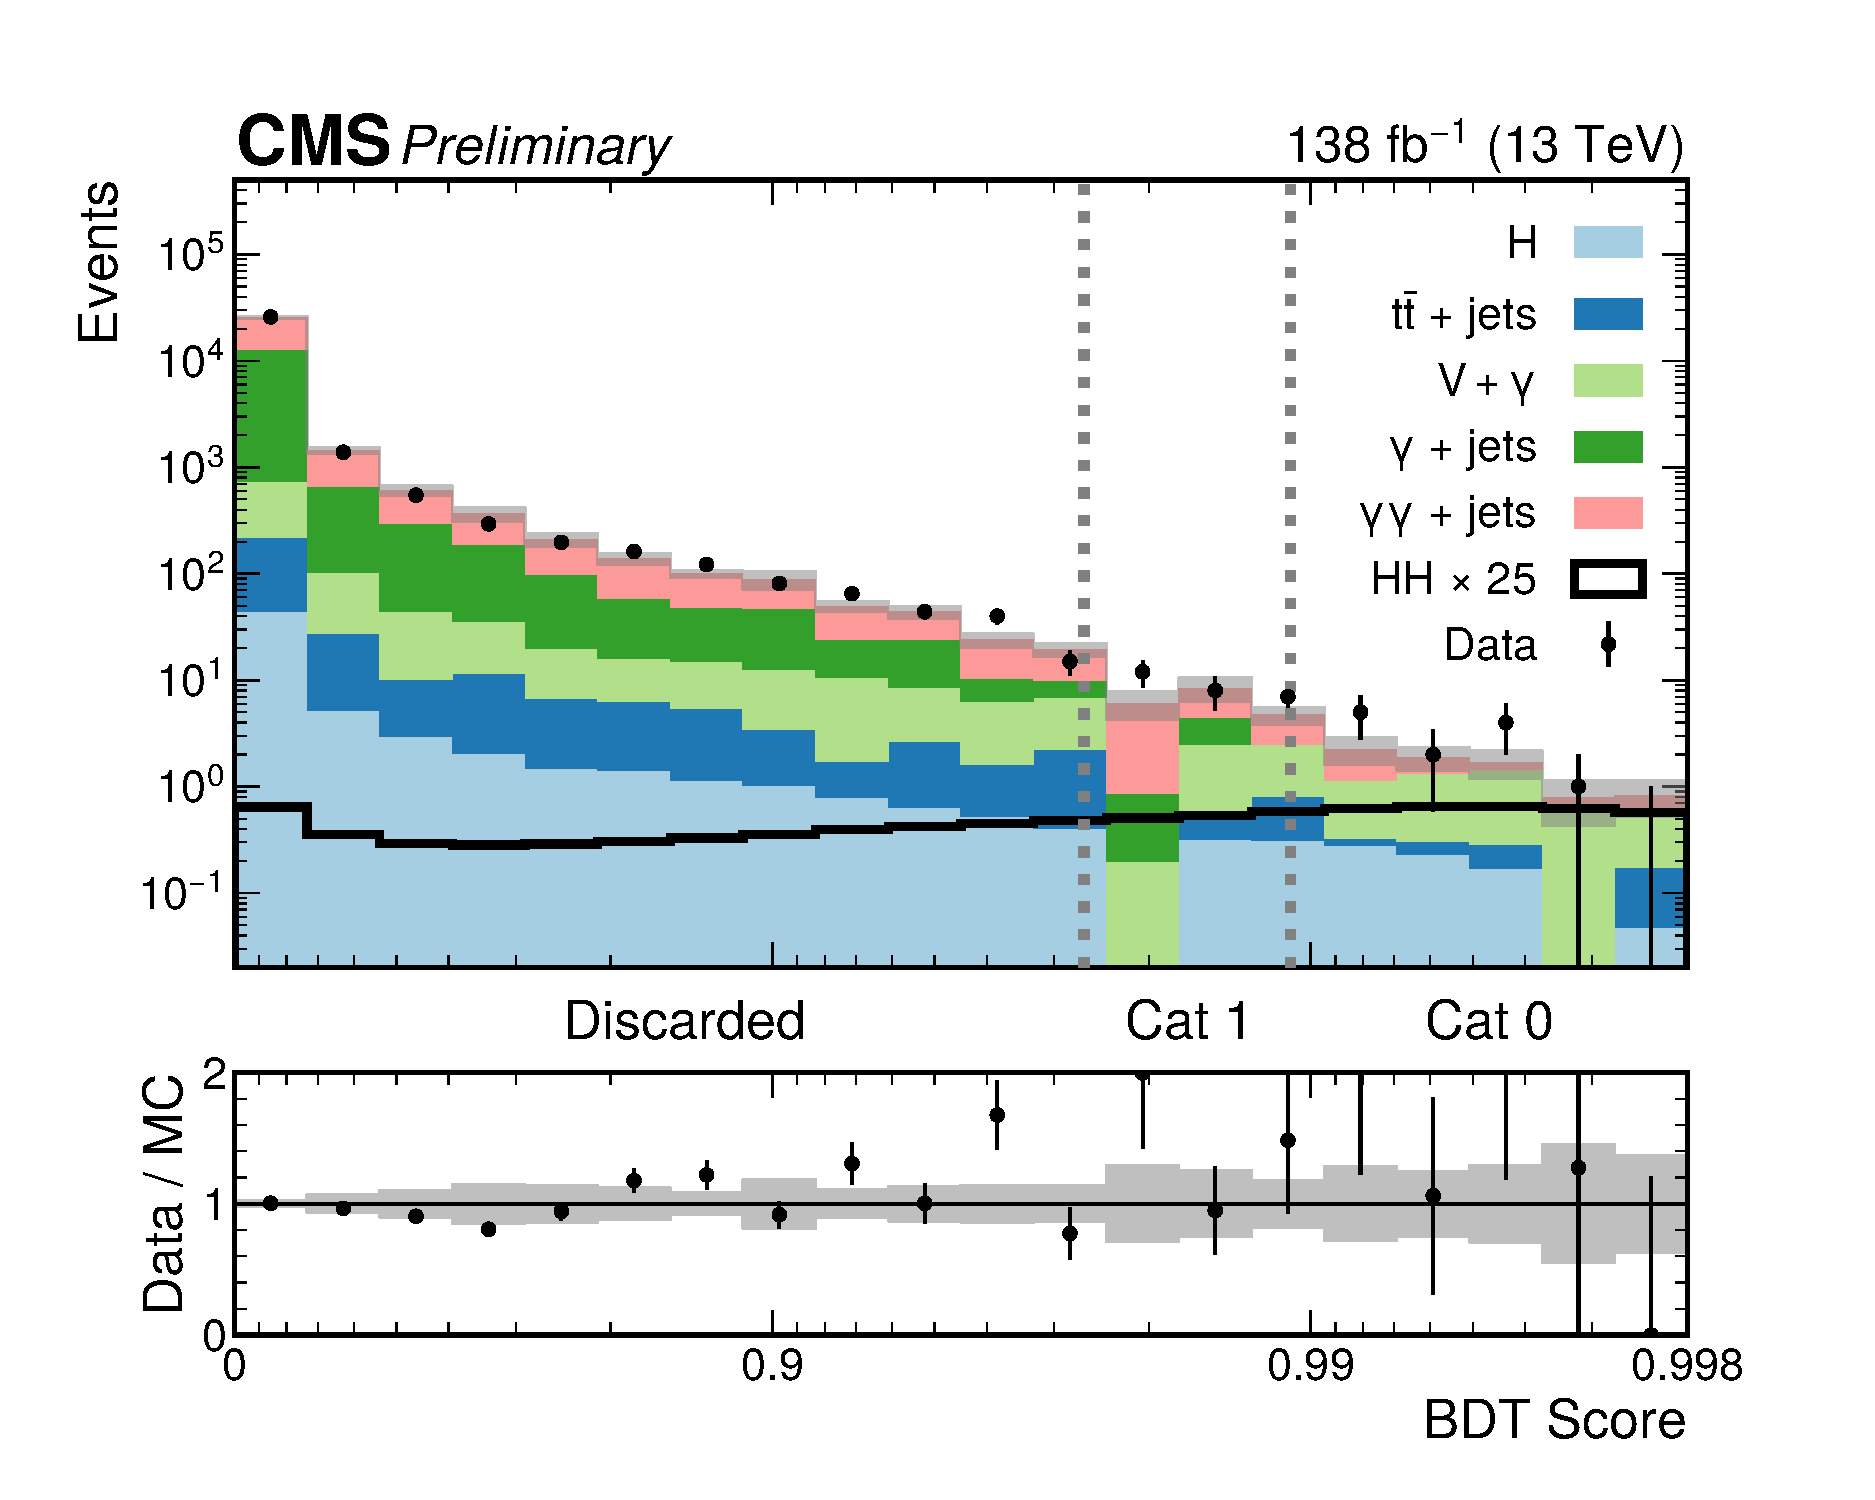
\includegraphics[width=.555\textwidth]{/home/bruno/org/PhD/Thesis/figures/ggtt_BDT.pdf}
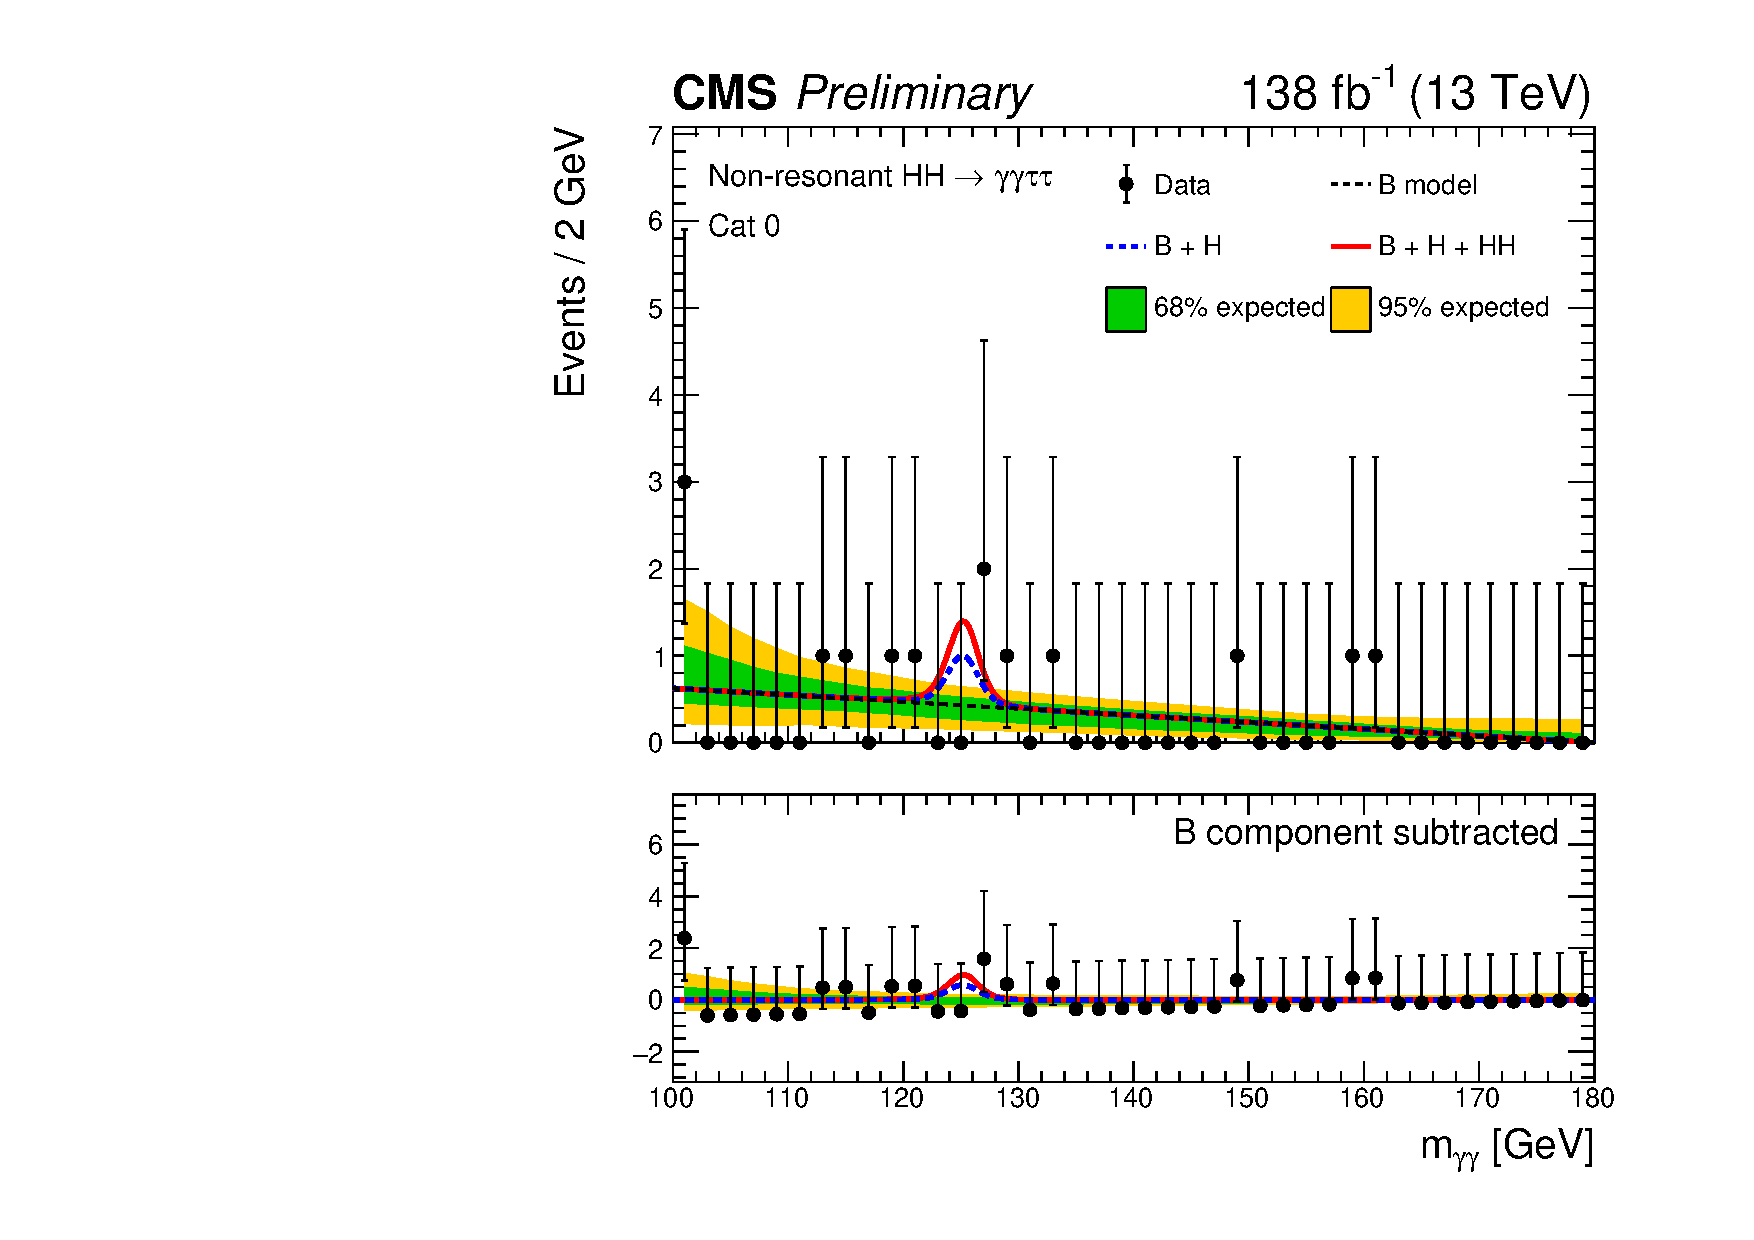
\includegraphics[width=.445\textwidth]{/home/bruno/org/PhD/Thesis/figures/ggtt_result.pdf}
\caption{\label{fig:ggtt_results}Results of the \(\gamma \gamma \tau \tau\) nonresonant analysis. \emph{Left)} Distribution of the BDT scores used for the event categorization from data and predictions from MC simulation. \emph{Right)} Data points and signal-plus-background models for the most sensitive analysis category, where the lower panel in each plot shows the residual signal yield after subtraction of the background. Taken from \cite{gammagammatautau}.}
\end{figure}
\subsubsection{ZZ, ZH and future techniques}
\label{sec:orgaf58df2}
\begin{enumerate}
\item The \zzzhbbbb{} analysis
\label{sec:org4e06be1}
The ZZ and ZH processes represent standard candles to validate the HH analyses, given that they have cross-sections 31 and 8 times larger than the \ac{SM} ones, respectively, and are therefore expected to be observed before the \bbbb{} process.
The recently published resolved \zzzhbbbb{} analysis \cite{zz_zh_bbbb} uses a series of advanced background estimation techniques to successfully validate a \ac{QCD} estimate using synthetic datasets (\cref{sec:qcd_bkgd_problem}).

In order to model the \ac{QCD} background, a control region is defined by requiring three b-tagged jets instead of four.
The dataset thus obtained, so as to reproduce the \ac{SR}, is weighted by two sets of weights, ti account for additional jet activity and subsisting kinematic mismatches.
The weights are derived in a di-jet mass sideband.

The analysis introduces a \ac{DNN} architecture especially designed to handle the b-quark pairing combinatorics: the \ac{HCR} network.
A detailed explanation is outside the scope of this work, but suffices to say that it is used to discriminate signal from background, to define the background model kinematic weights, and to differentiate \ac{QCD} from \(\ttbar{}\) in the technique of \cref{sec:hemisphere_mixing}.

The final fit is validated using the synthetic dataset, without statistical fluctuations, and using one of the mixed models as the four-tag data. Systematics behaved as expected and the result was compatible with a zero signal strength.
The observed (expected) 95\% CL upper limits on the production cross sections correspond to 3.8 (3.8) and 5.0 (2.9) times the \ac{SM} prediction, for the \zzbbbb{} and \zhbbbb{} processes, respectively.
The analysis indicates that ZH will likely be ovserved first.
\item The problem with \ac{QCD} simulations
\label{sec:orgd4439ba}
\label{sec:qcd_bkgd_problem}

Many analysis in CMS include quark- or gluon- induced jets in their final state particles.
This is also the case for some HH analysis, including the most sensitive ones (since they include a pair of b-jets) \cite{higgs_bbtautau_nonres,bbgg_cms,bbbb_resolved_cms,bbbb_boosted_cms}.
\ac{QCD} backgrounds are often significant, and sometimes dominant, as in \bbbb{} analysis, where the second most common source of background, \(\ttbar\), is almost an order of magnitude less common.
Unfortunately, currently available \ac{QCD} simulations lack the required precision and statistics for a robust background estimate, particulary in the higher energy distribution tails.

Data-driven methods are therefore usually employed to model the \ac{QCD} background.
These usualy take the form of ``ABCD-like'' methods, where \acp{CR} are defined in such a way as to ensure orthogonality with respect to the \ac{SR}.
Some variants exist, such as (possibly high-dimensional) ``alphabet'' \cite{corcodilos_thesis} and ``fake factor'' \cite{fake_factor_method,higgs_bbtautau_hy} methods, but the general principles, especially in the context of this work, are similar.
The basic idea is to find fully uncorrelated variables upon which the \ac{SR} selection depends on, and invert the cuts to obtain signal-free regions.
The latter can be used to estimate both the shape and the normalization of the \ac{QCD} background in the \ac{SR}, without using it directly.

To give an example, in the most recent \bbtt{} non-resonant analysis \cite{higgs_bbtautau_nonres}, the \(\tau\) isolation and the relative sign of the charges of the two leptons are used to create three \acp{CR} around the analysis \ac{SR} (opposite-charged leptons and well isolated \(\tau\)'s). Defining B, C and D as three \acp{CR} where B has equally charged leptons and tight isolation, C has opposite charged leptons and loose isolation, and D has both cuts inverted, the shape of the \ac{SR} can be inferred either by B or C and the normalization by B/D or C/D, respectively.
In the resolved \bbbb{} analysis \cite{bbbb_resolved_cms}, instead, the control regions are defined based on the invariant mass of the two Higgses and on the number of b-tagged jets.
The \ac{SR}, having 4 b-jets, has its \ac{QCD} background modeled from events in \acp{CR} with 3-bjets.
It is assumed that kinematic properties are similar between \acp{CR} and the \ac{SR}. 

In all cases, the background is derived in a signal-free region, and thus requires an extrapolation to a different region of the phase-space.
In order to validate the extrapolation, a \ac{VR} is usually employed.
However, the definition of an additional region will necessarily deplete the signal region.
Additionally, the extrapolation cannot be directly tested, since the \ac{VR} differs from the signal region inasmuch as it will not be signal-enriched.
Finally, both \acp{CR} and \acp{VR} often have low statistics, and become a dominant source of systematic uncertainties.
Indeed, finite data in \acp{VR} imply an ``inherent limitation on the capability to validate the performance of the background model'' \cite{zz_zh_bbbb}.
There is therefore a need to develop new methods to estimate and validate the \ac{QCD} background estimation that are not sensitive to low statistics.
In addition, it would be beneficial to directly test the ABCD extrapolation in the \ac{SR}.
\item Hemisphere mixing
\label{sec:orgb509fd5}
\label{sec:hemisphere_mixing}

The hemisphere mixing technique \cite{hemisphere_mixing} first creates a library of ``hemispheres'', which arise from the splitting of events along the plane orthogonal to the transverse thrust axis.
The latter is in turn defined as the axis where the sum of the absolute values of the \(\pt\) projections of the all the jets in the event is maximal.
The splitting is done using a sample of events with four b-tagged jets, thus ``pure'' in signal events.
For each hemisphere a set of four variables is calculated: mass, longitudinal momentum, and transverse momentum perpendicular and parallel to the thrust axis.
A second pass on data mixes pairs of hemispheres by minimizing the distance of two hemispheres in terms of a normalized sum of the summary variables.
The two hemispheres must belong to different events.

The paper here discussed \cite{zz_zh_bbbb} contributes with two improvements to the original hemisphere mixing technique.
Firstly, the mixing step is performed with 3-tagged data in order to increase statistics and make (4-tagged) signal contamination negligible.
Statistics are also increased by lowering the b-tag \ac{WP} used on the three jets.
Secondly, the non-negligible presence of \(\ttbar{}\) events is mitigated by removing such events from the mixing stage.
This is done event-by-event via a classification with the \ac{HCR} network, which calculates the probability P(M) for each event to be multijet, where a random number X is generated between 0 and 1. If \(\text{X} > \text{P(M)}\), the event is rejected.

For the validation of the background model, we have to ensure the size of the synthetic dataset is comparable to the one used for the model.
The hemisphere dataset is thus sub-sampled, and 15 separate mixed models are formed, given the available statistics.
Systematic uncertainties of the \ac{QCD} modeling are determined using the synthetic dataset in three different ways:
\begin{enumerate}
\item Differences between mixed models, arising from limited statistics, are quantified by using their average;
\item The background model is compared with the mixed models in the signal region;
\item An unconstrained signal template is added to the signal + background fit to verify if a spurious signal can be mimicked by the background model. This fit is compared with a background-only fit and found to be in agreement.
\end{enumerate}

Importantly, and despite not yet being used in the most recent \bbbb{} results, a principled and precise way of measuring the most important systematics directly in the \ac{SR} is now available.
We note that, given appropirate modifications, a similar method could be extended to the \bbtt{} analysis.
\end{enumerate}
\subsubsection{Indirect searches}
\label{sec:org31299a9}
\label{sec:indirect_searches}

An alternative method was developed to extract information on the trilinear Higgs coupling without using Higgs boson pair production.
Once can explore \ac{NLO} electroweak loops present in single Higgs production featuring the trilinear Higgs vertex.
It has also been proposed to use higher-order diagrams of \ac{EW} processes, such as \(\mw\) and \(\sint\) measurements, with the same goal \cite{indirect_searches_ew}.
The production modes with the largest kinematic dependence on \(\lh{3}\) are \tth{} and \vh{} \cite{indirect_searches2}, with differences of up to 10\%.

The bounds obtained from indirect searches are competitive with the ones from di-Higgs production \cite{indirect_searches3}, and provide additional constraints for single Higgs couplings (see \cref{sec:combinations}).
Nevertheless, departures of the Higgs self-coupling from its \ac{SM} prediction signal the existence
of new dynamics that, in general, would leave an imprint on other Higgs couplings.
The importance of a global fit is therefore two-fold, namely to assess the robustness of the studies that take into account deformations exclusively in the Higgs trilinear coupling, and to single out the sensitivity on the single-Higgs couplings that is required to minimise the impact of the possible correlations \cite{hllhc_physics}.

Single and double Higgs processes are extremely complementary \cite{indirect_searches4}.

\cite{indirect_searches1}


\begin{figure}
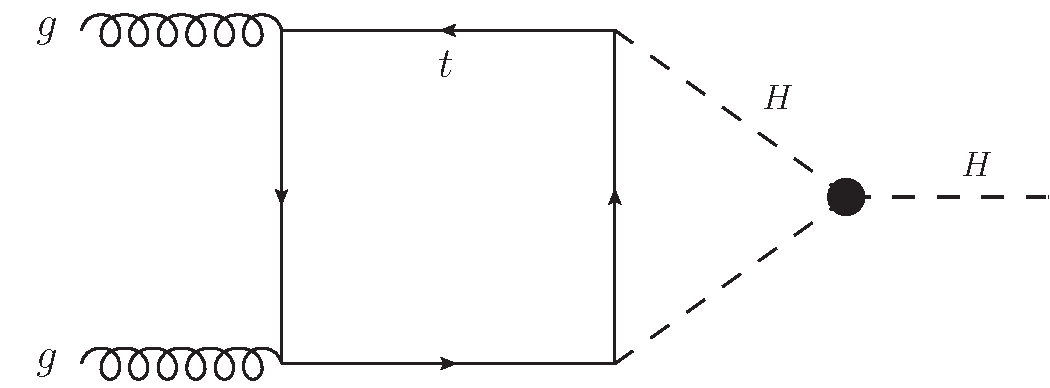
\includegraphics[width=.45\textwidth]{/home/bruno/org/PhD/Thesis/figures/intro/single_higgs_indirect1.pdf}
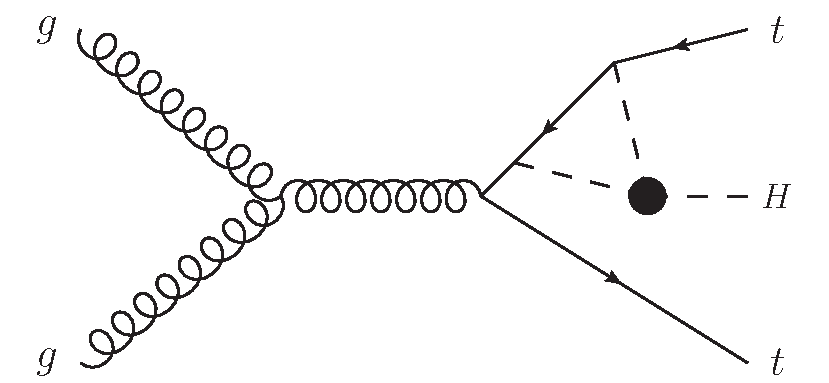
\includegraphics[width=.45\textwidth]{/home/bruno/org/PhD/Thesis/figures/intro/single_higgs_indirect3.pdf}
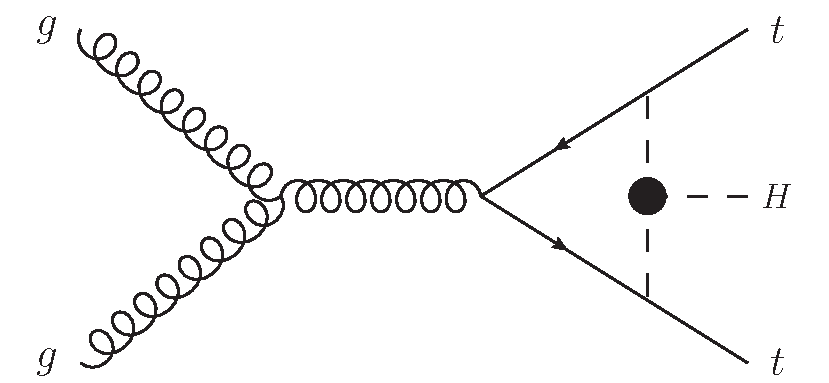
\includegraphics[width=.45\textwidth]{/home/bruno/org/PhD/Thesis/figures/intro/single_higgs_indirect4.pdf}
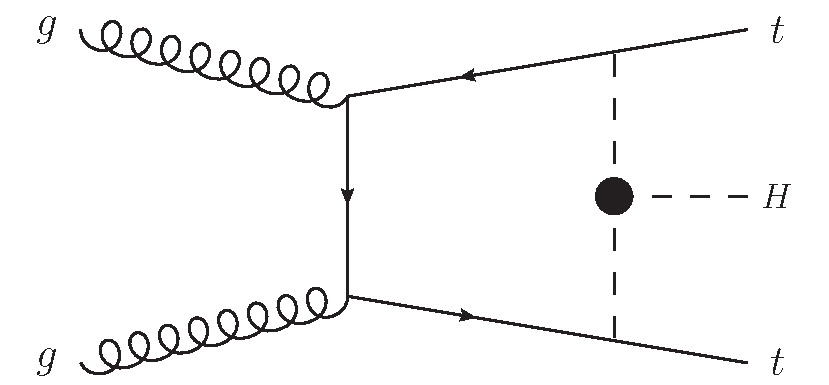
\includegraphics[width=.45\textwidth]{/home/bruno/org/PhD/Thesis/figures/intro/single_higgs_indirect5.pdf}
\caption{\label{fig:single_higgs_indirect_production}Examples of single Higgs boson production processes contributing to the Higgs boson self-coupling. The top left one represent \ac{ggF} while the remaining refer to \tth{}. Taken from \cite{indirect_searches1}.}
\end{figure}

\begin{figure}
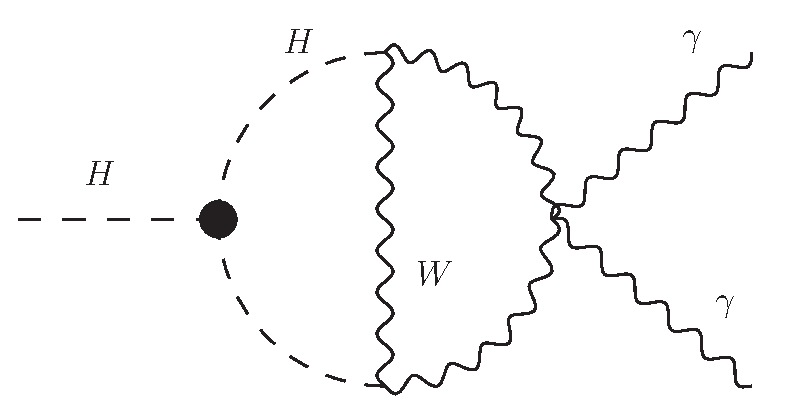
\includegraphics[width=.45\textwidth]{/home/bruno/org/PhD/Thesis/figures/intro/single_higgs_indirect7.pdf}
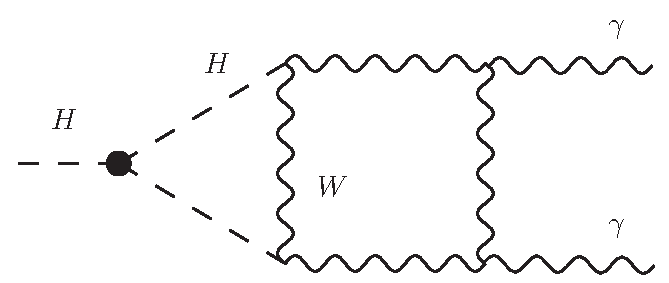
\includegraphics[width=.45\textwidth]{/home/bruno/org/PhD/Thesis/figures/intro/single_higgs_indirect2.pdf}
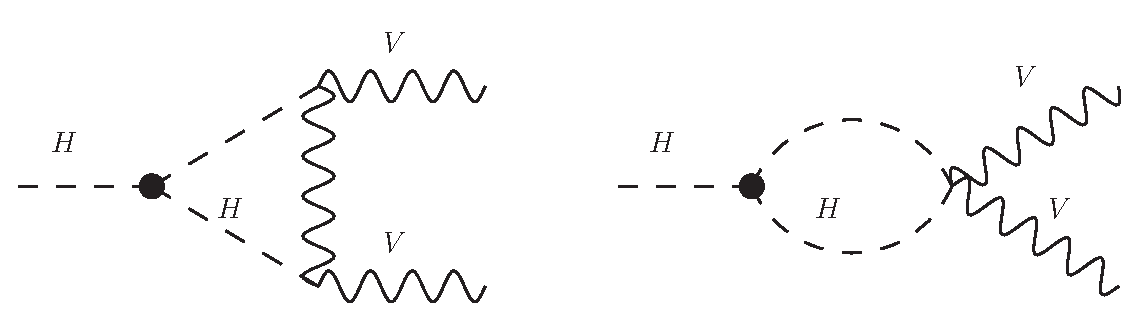
\includegraphics[width=.9\textwidth]{/home/bruno/org/PhD/Thesis/figures/intro/single_higgs_indirect6.pdf}
\caption{\label{fig:single_higgs_indirect_decay}Examples of single Higgs boson decay processes contributing to the Higgs boson self-coupling. The diagrams in the top (bottom) row refer to \ac{NLO} \(\gamma\gamma\) (\(VV\)) decays. Taken from \cite{indirect_searches1}.}
\end{figure}
\subsubsection{Combinations}
\label{sec:org7f00be9}
\label{sec:combinations}

@mention impact of bb\(\tau \tau\)@

The most up-to-date Run2 HH combination constrains the observed (expected) HH cross-section to \(\xshh < 3.4\;(2.5)\;\xshhsm\), where the sensitivity is dominated by the \(4b\), \(bb\tau\tau\) and \(bb\gamma\gamma\) channels. The limit is also interpreted as a function of the \(\kl\) and \(\k2v\) coupling modifiers, measuring \(-1.24 < \kl < 6.49\) and \(0.67 < \kvv < 1.38\), respectively. Importantly, the latter result allows the exclusion of \(\kvv=0\) at 6.6 standard deviations.

\begin{figure}[htbp]
\centering
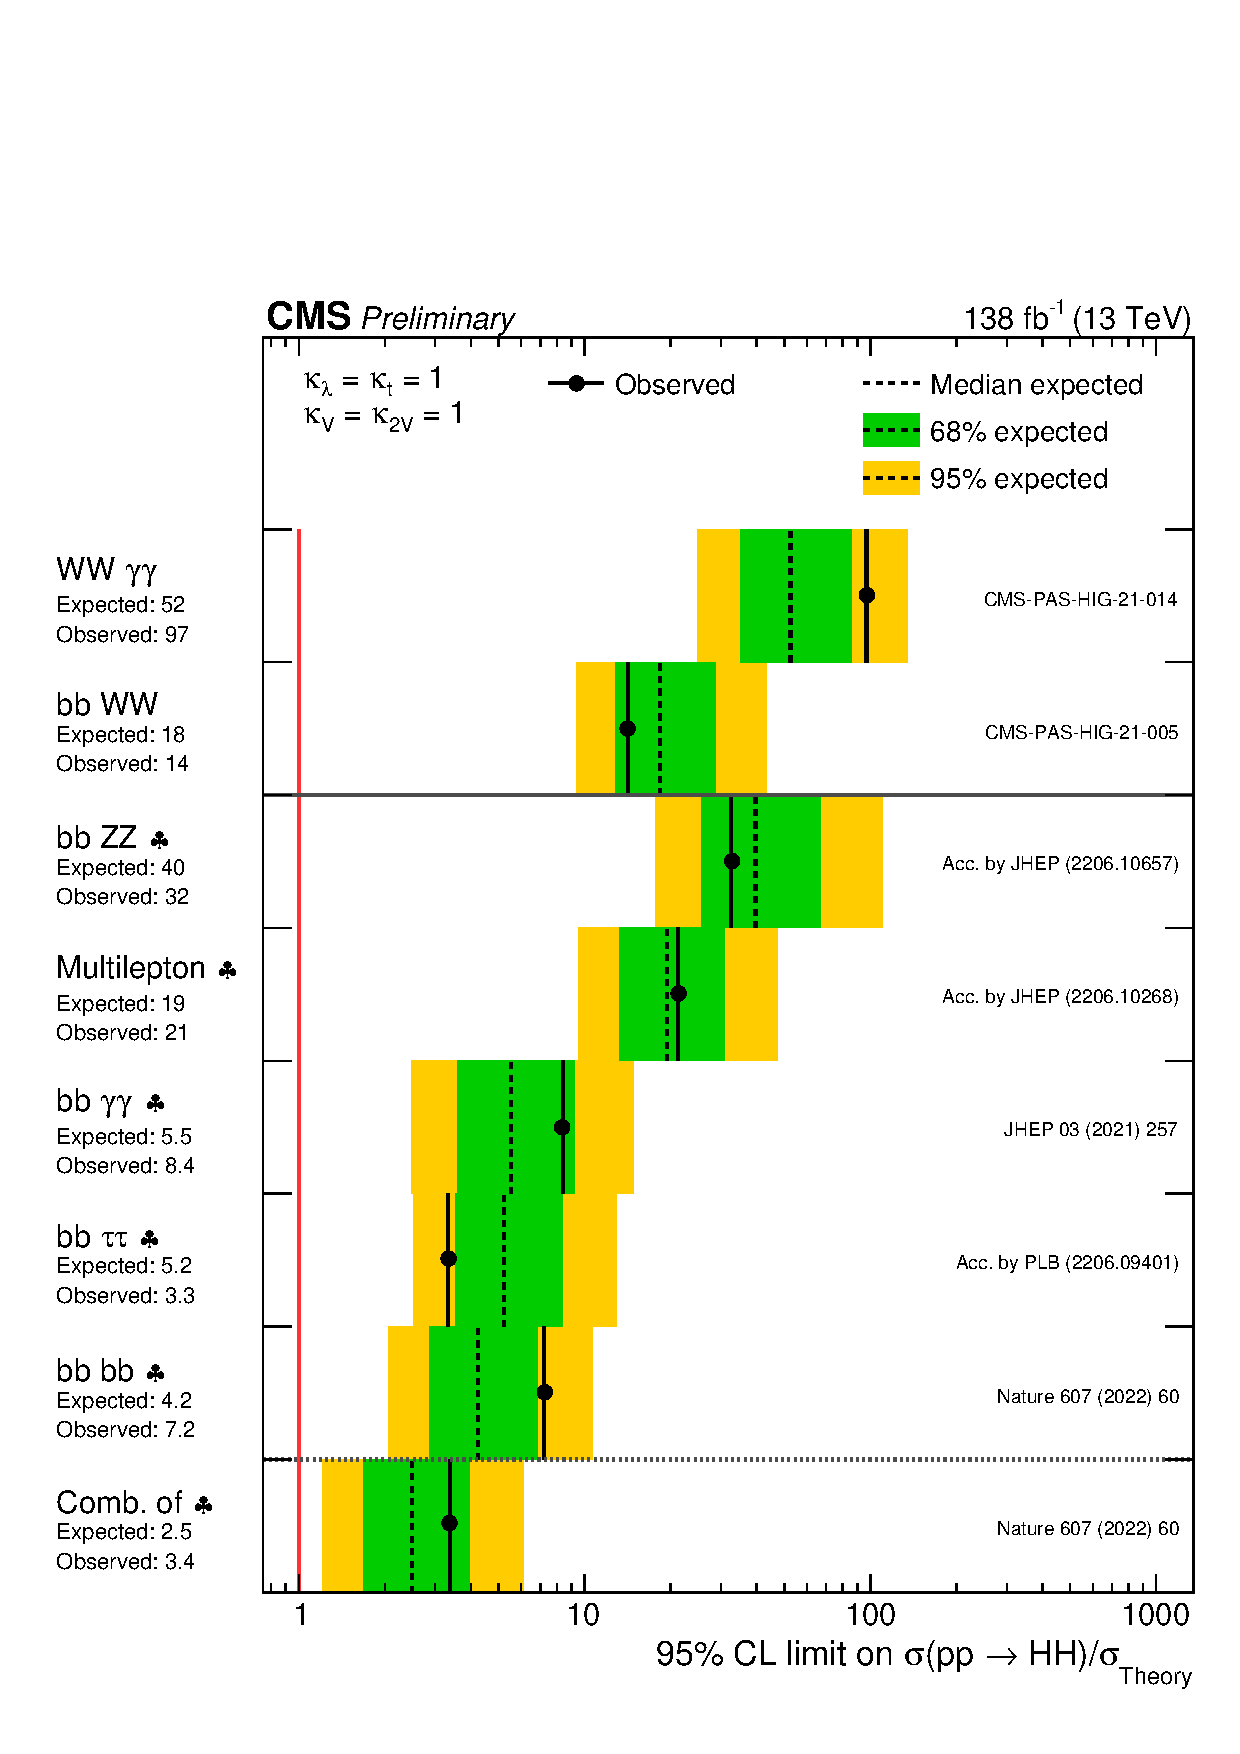
\includegraphics[width=.8\textwidth]{/home/bruno/org/PhD/Thesis/figures/intro/limits_HH_SM_Mar2023.pdf}
\caption{\label{fig:HH_nonres_comb_xsec}Upper limits at 95\% confidence level on the SM signal strength \(\mu = \xshh / \xshhsm\). The inner (green) band and the outer (yellow) bands indicate the regions containing 68\% and 95\%, respectively, of the limits on \(\mu\) expected under the background-only hypothesis. The quoted expected upper limits are evaluated with the postfit values of the uncertainties. Figure taken from \cite{summary_hig_twiki}.}
\end{figure}

\begin{figure}
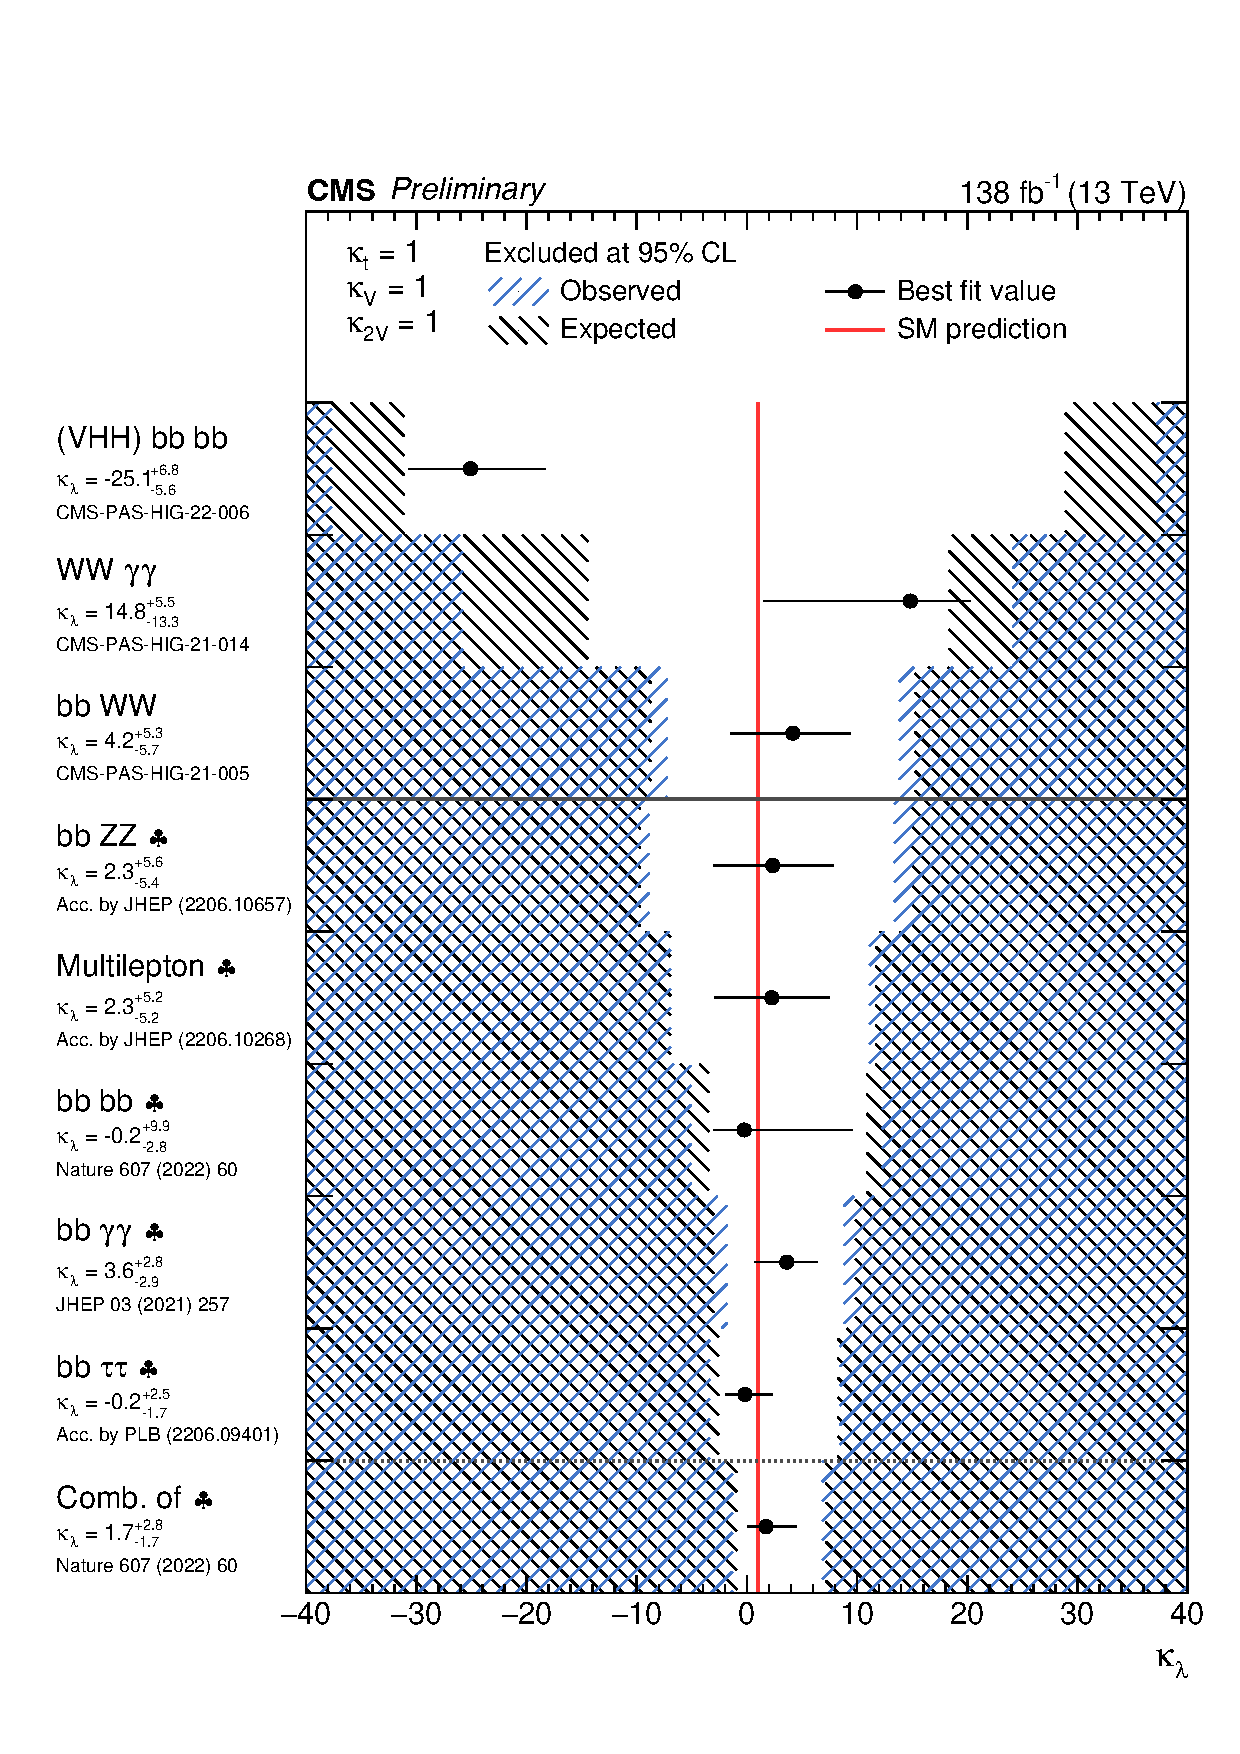
\includegraphics[width=.5\textwidth]{/home/bruno/org/PhD/Thesis/figures/exclusion_kl_Mar2023.pdf}
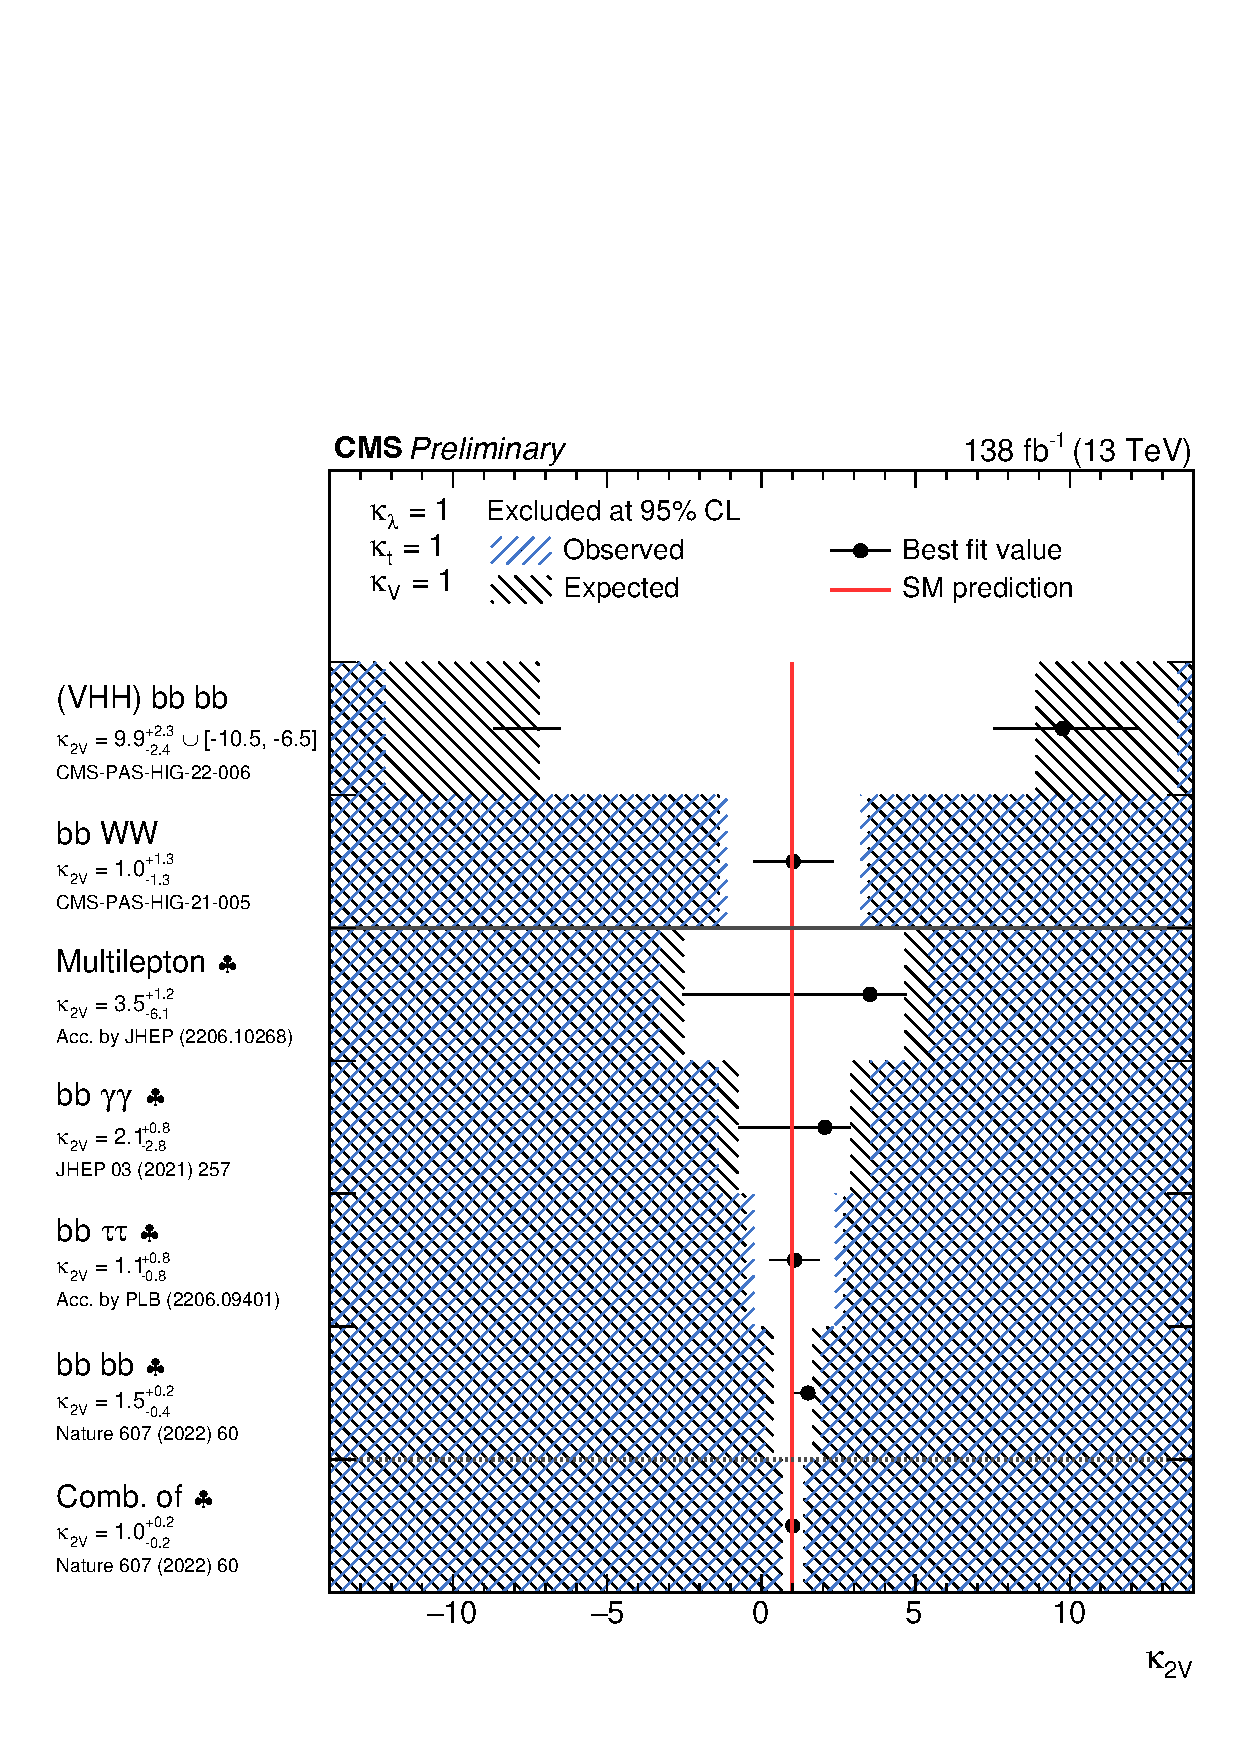
\includegraphics[width=.5\textwidth]{/home/bruno/org/PhD/Thesis/figures/exclusion_C2V_Mar2023.pdf}
\caption{\label{fig:HH_nonres_comb_c2v}95\% confidence intervals on \(\kl\) (left) and \(\kvv\) (right) superimposed by the best fit value on this parameter. The blue (black) hashed band indicates the observed (expected) excluded regions, respectively. The band around the best fit value corresponds to the one sigma interval. The quoted expected upper limits are evaluated with the postfit values of the uncertainties. Results are taken from the references marked next to each individual measurement.}
\end{figure}

\begin{figure}
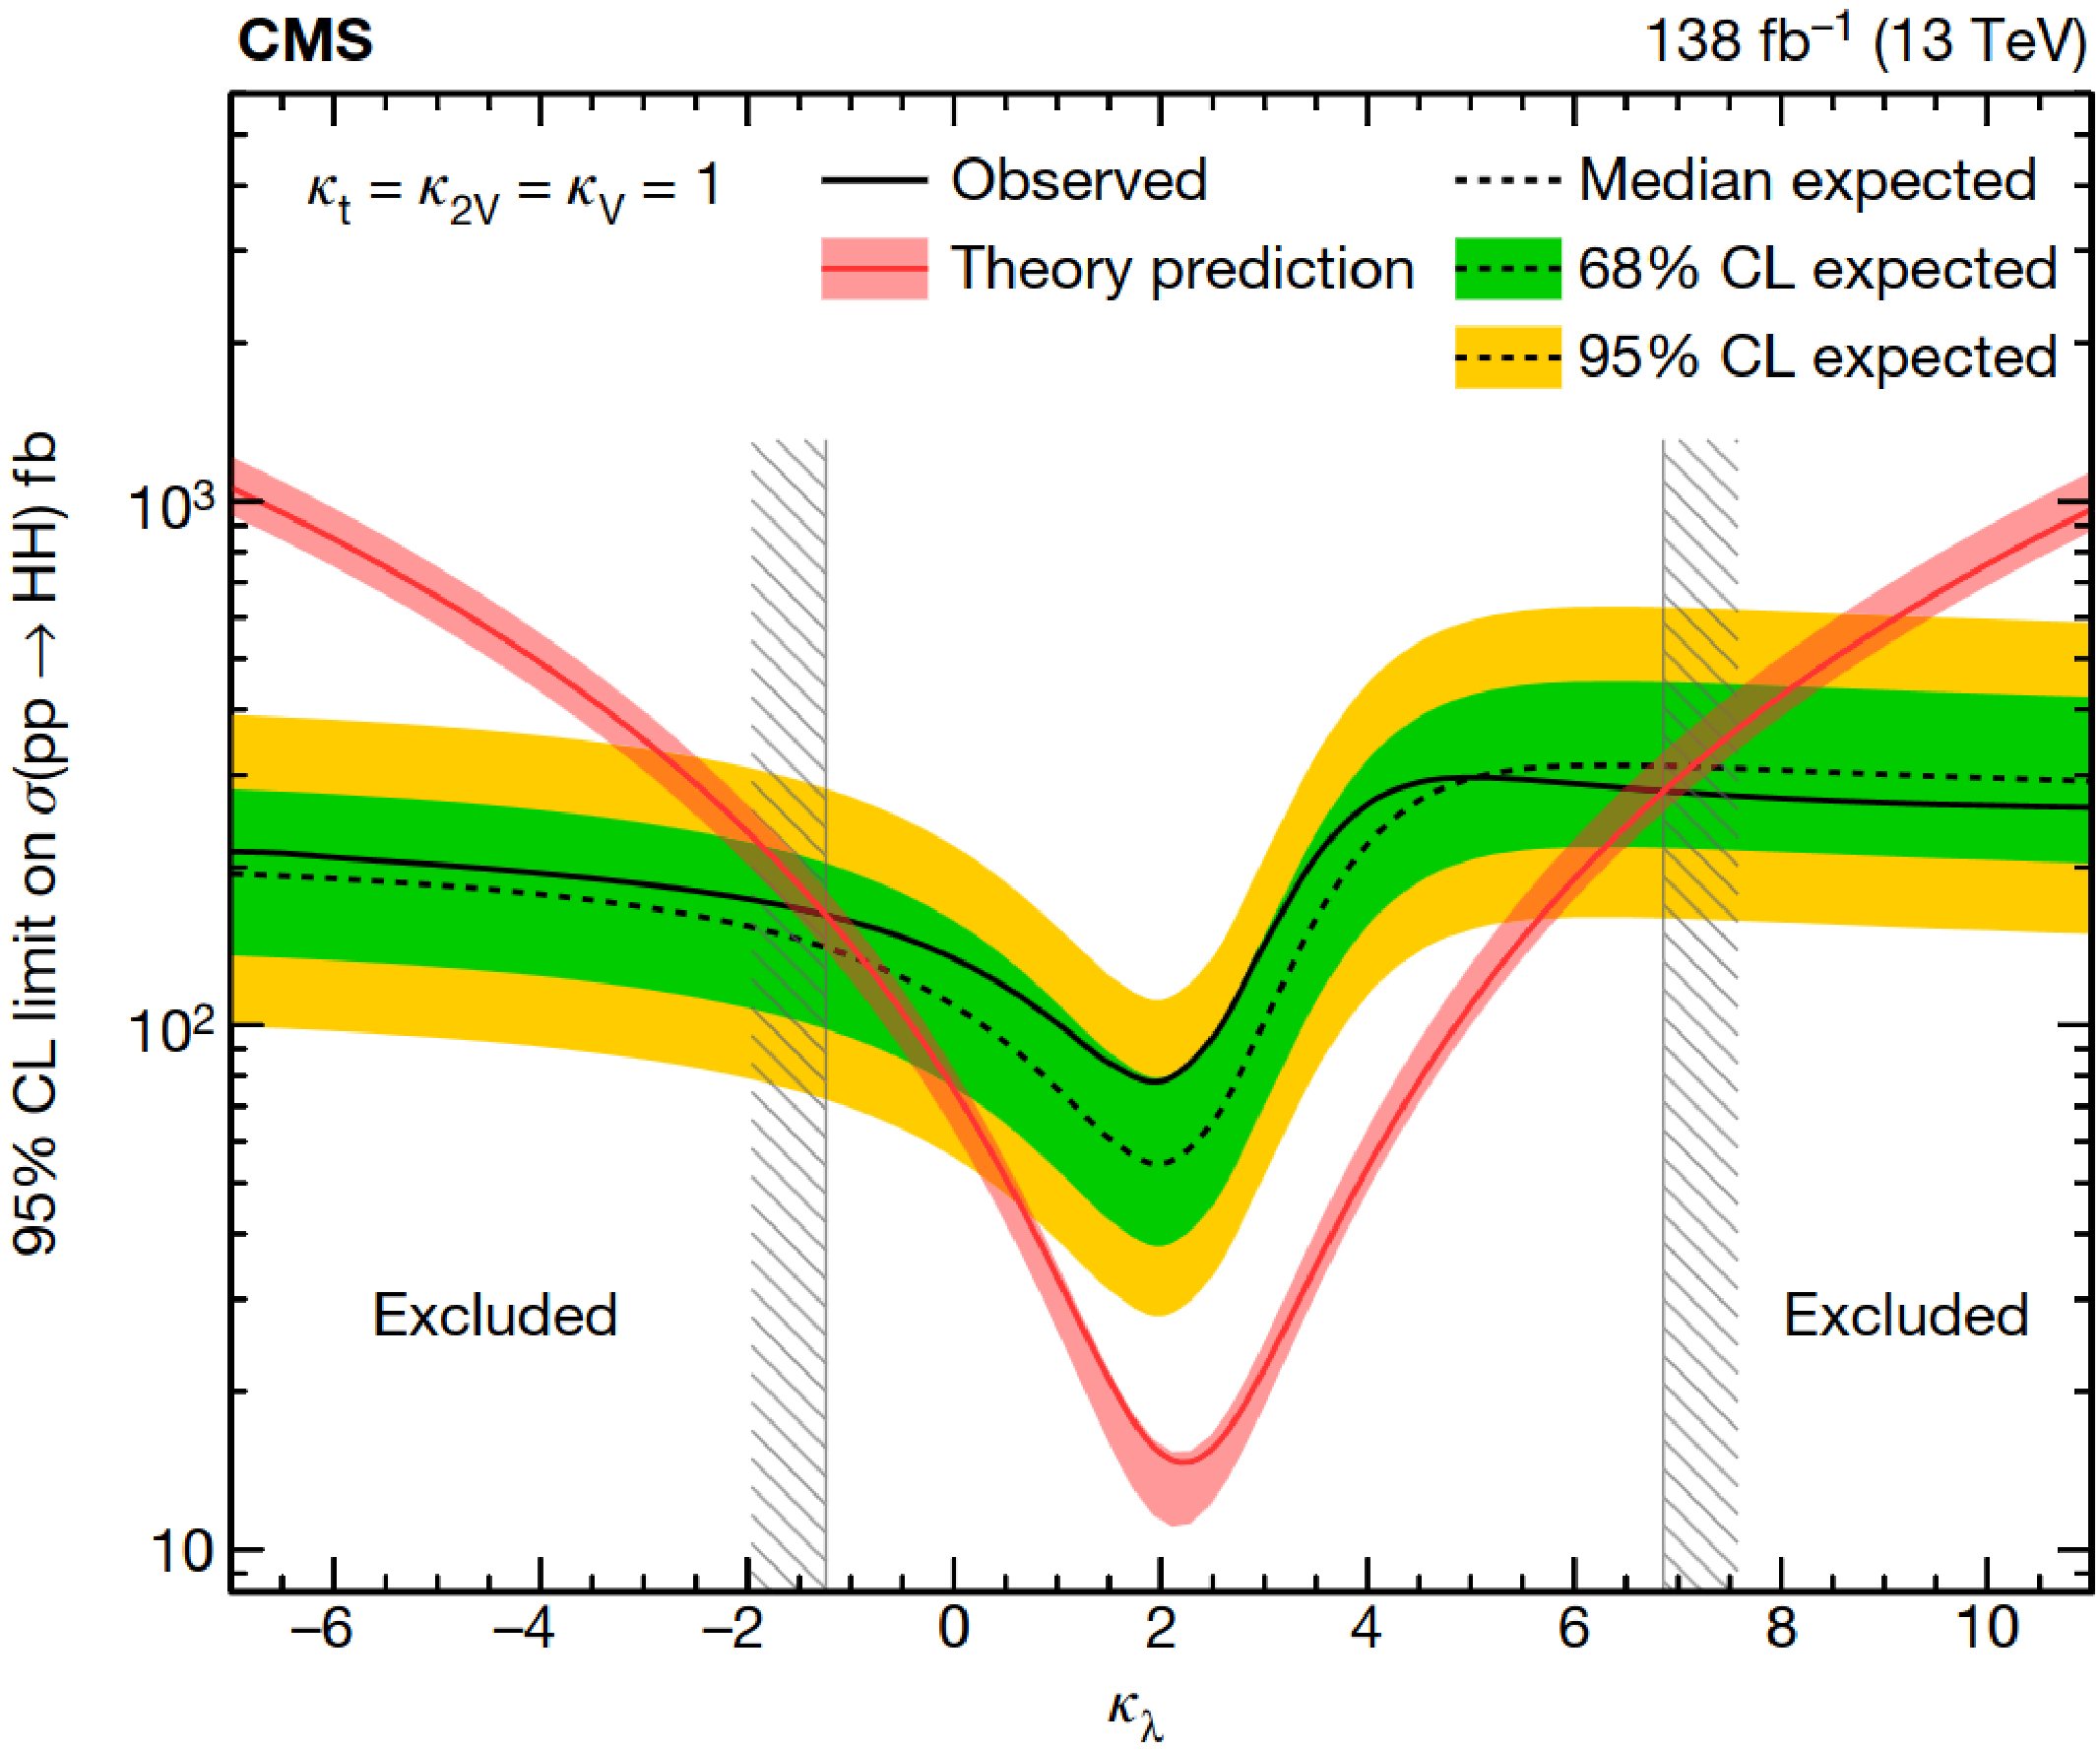
\includegraphics[width=.5\textwidth]{/home/bruno/org/PhD/Thesis/figures/scan_kl_nature.pdf}
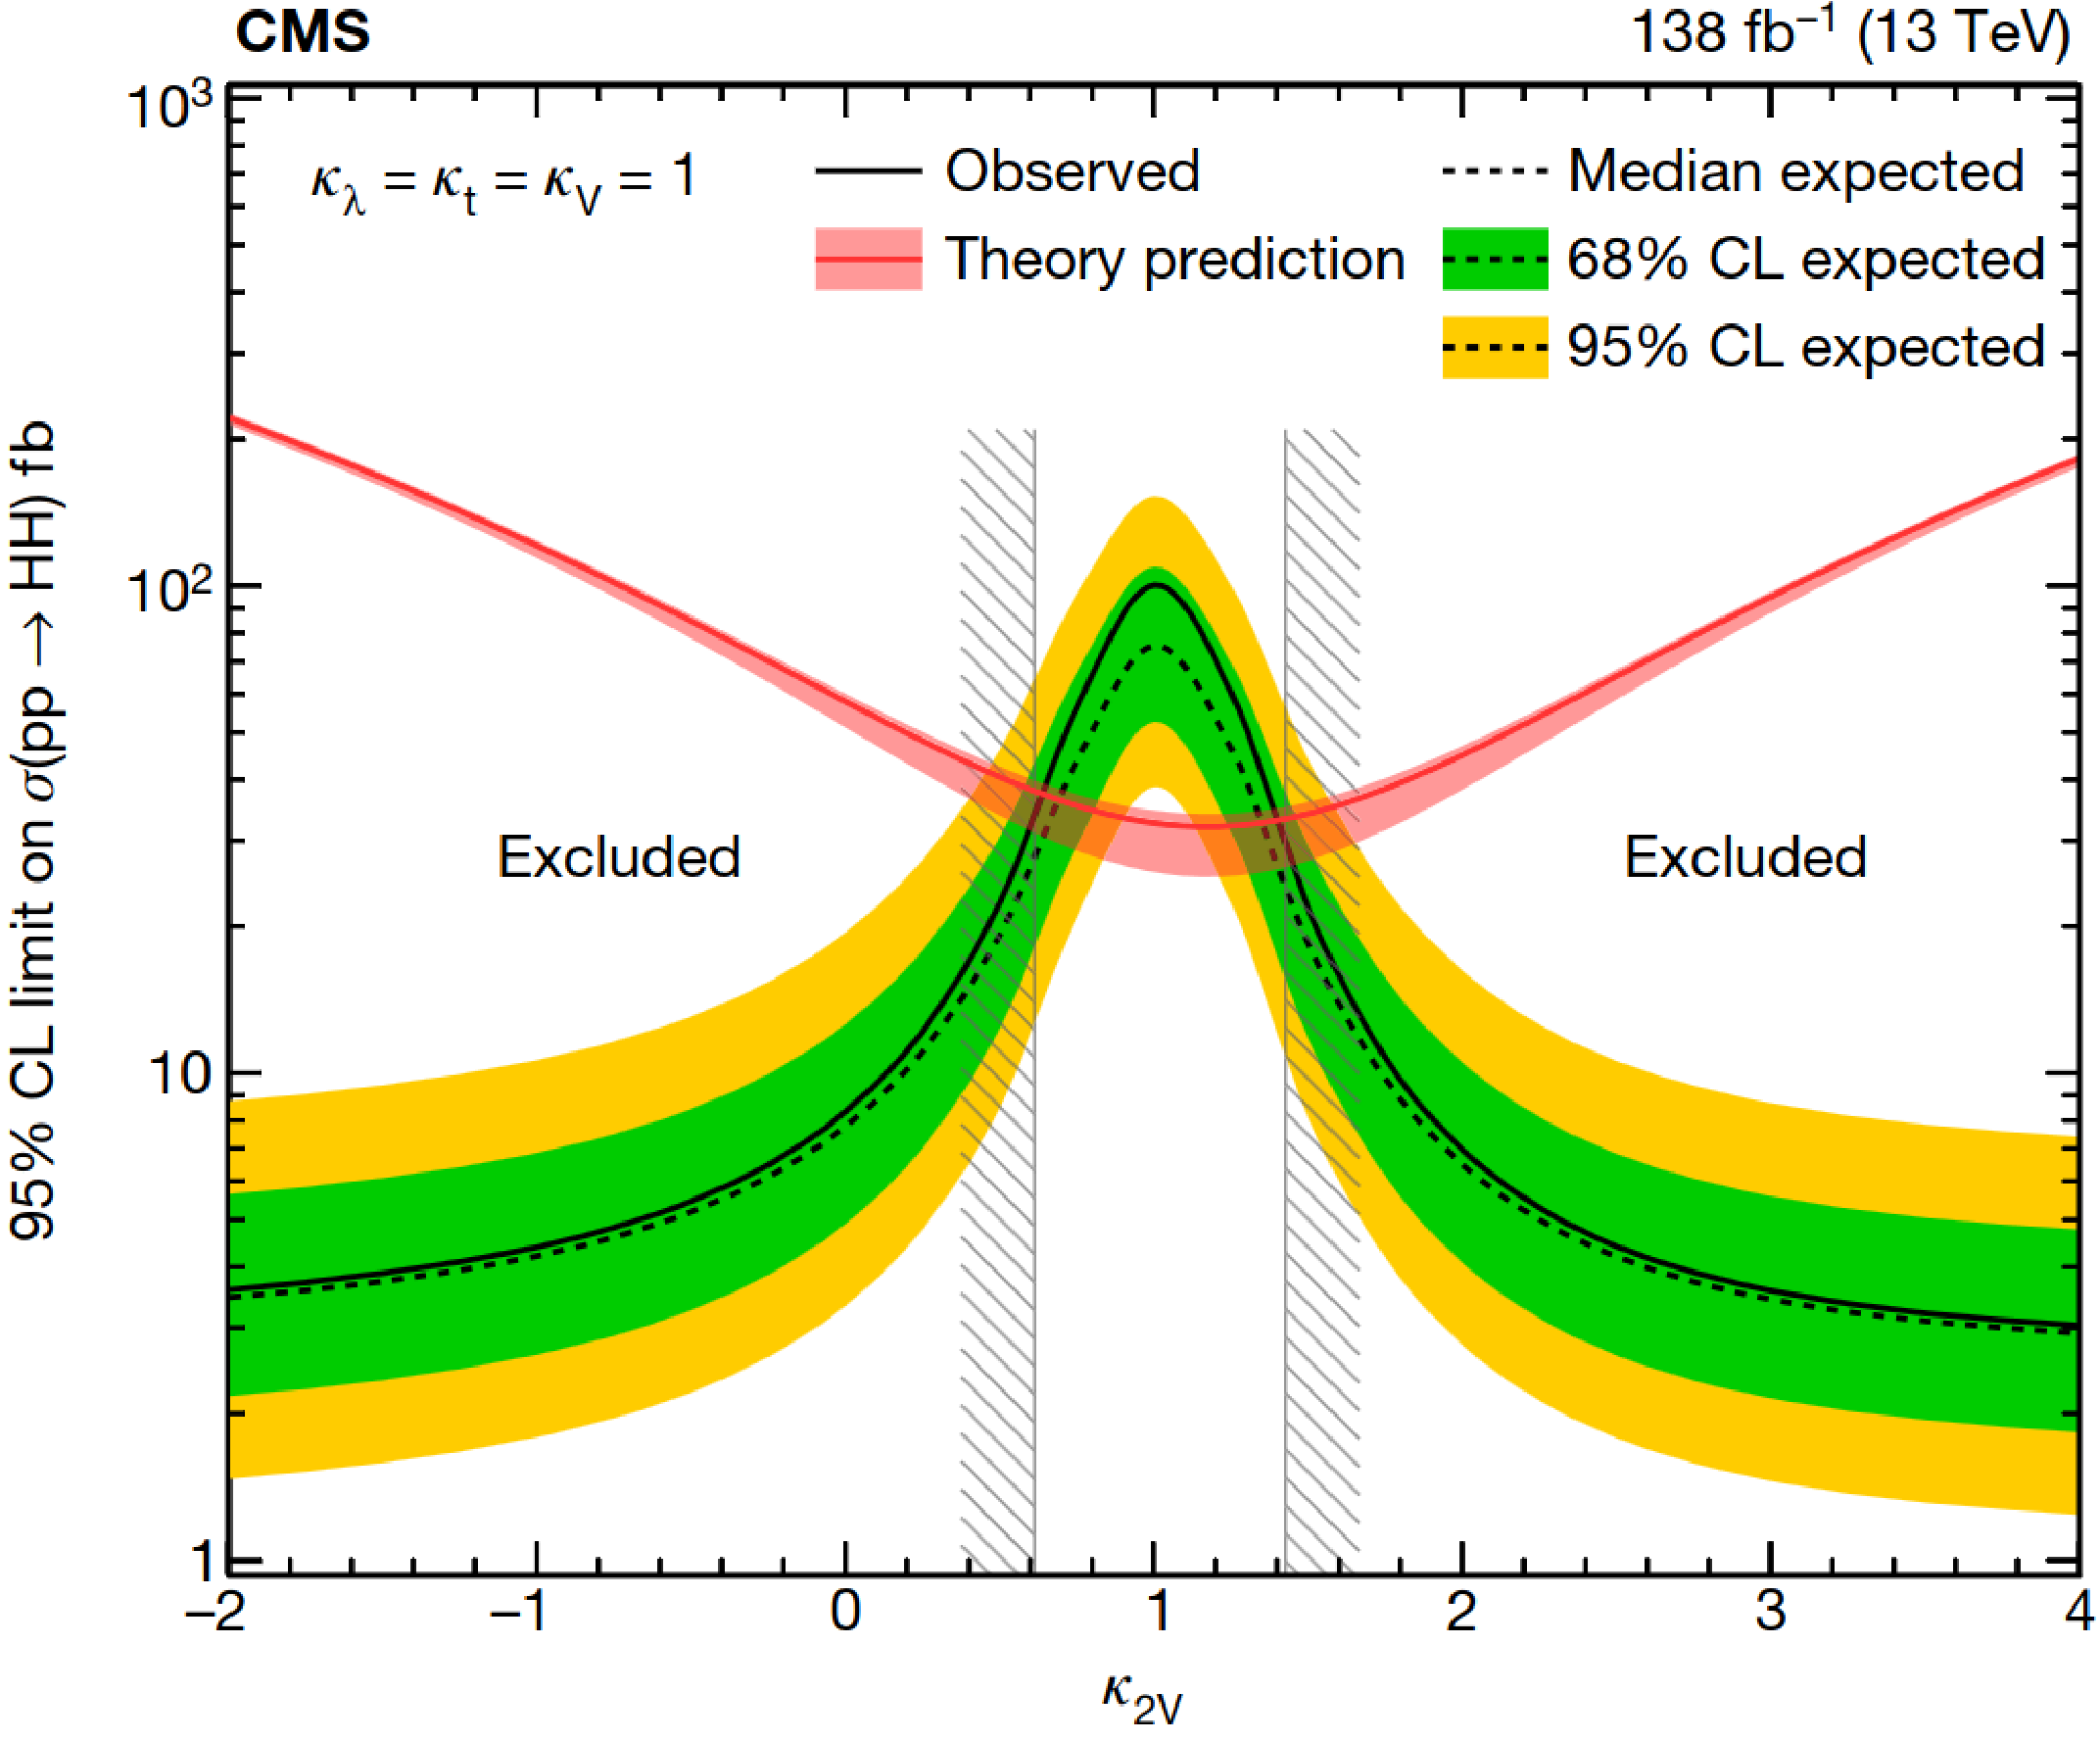
\includegraphics[width=.5\textwidth]{/home/bruno/org/PhD/Thesis/figures/scan_k2v_nature.pdf}
\caption{\label{fig:scan_comb_cms_nature}Combined expected and observed 95\% CL upper limits on the HH production cross-section for different values of \(\kl\) (left) and \(\kvv\) (right), assuming the SM values for the modifiers of Higgs boson couplings to top quarks and vector bosons. The green and yellow bands represent the 1\(\sigma\) and 2\(\sigma\) extensions beyond the expected limit, respectively; the red solid line (band) shows the theoretical prediction for the HH production cross-section (its 1\(\sigma\) uncertainty). The areas to the left and to the right of the hatched regions are excluded at the 95\% CL. Taken from \cite{higgs_10_years}.}
\end{figure}

\begin{figure}
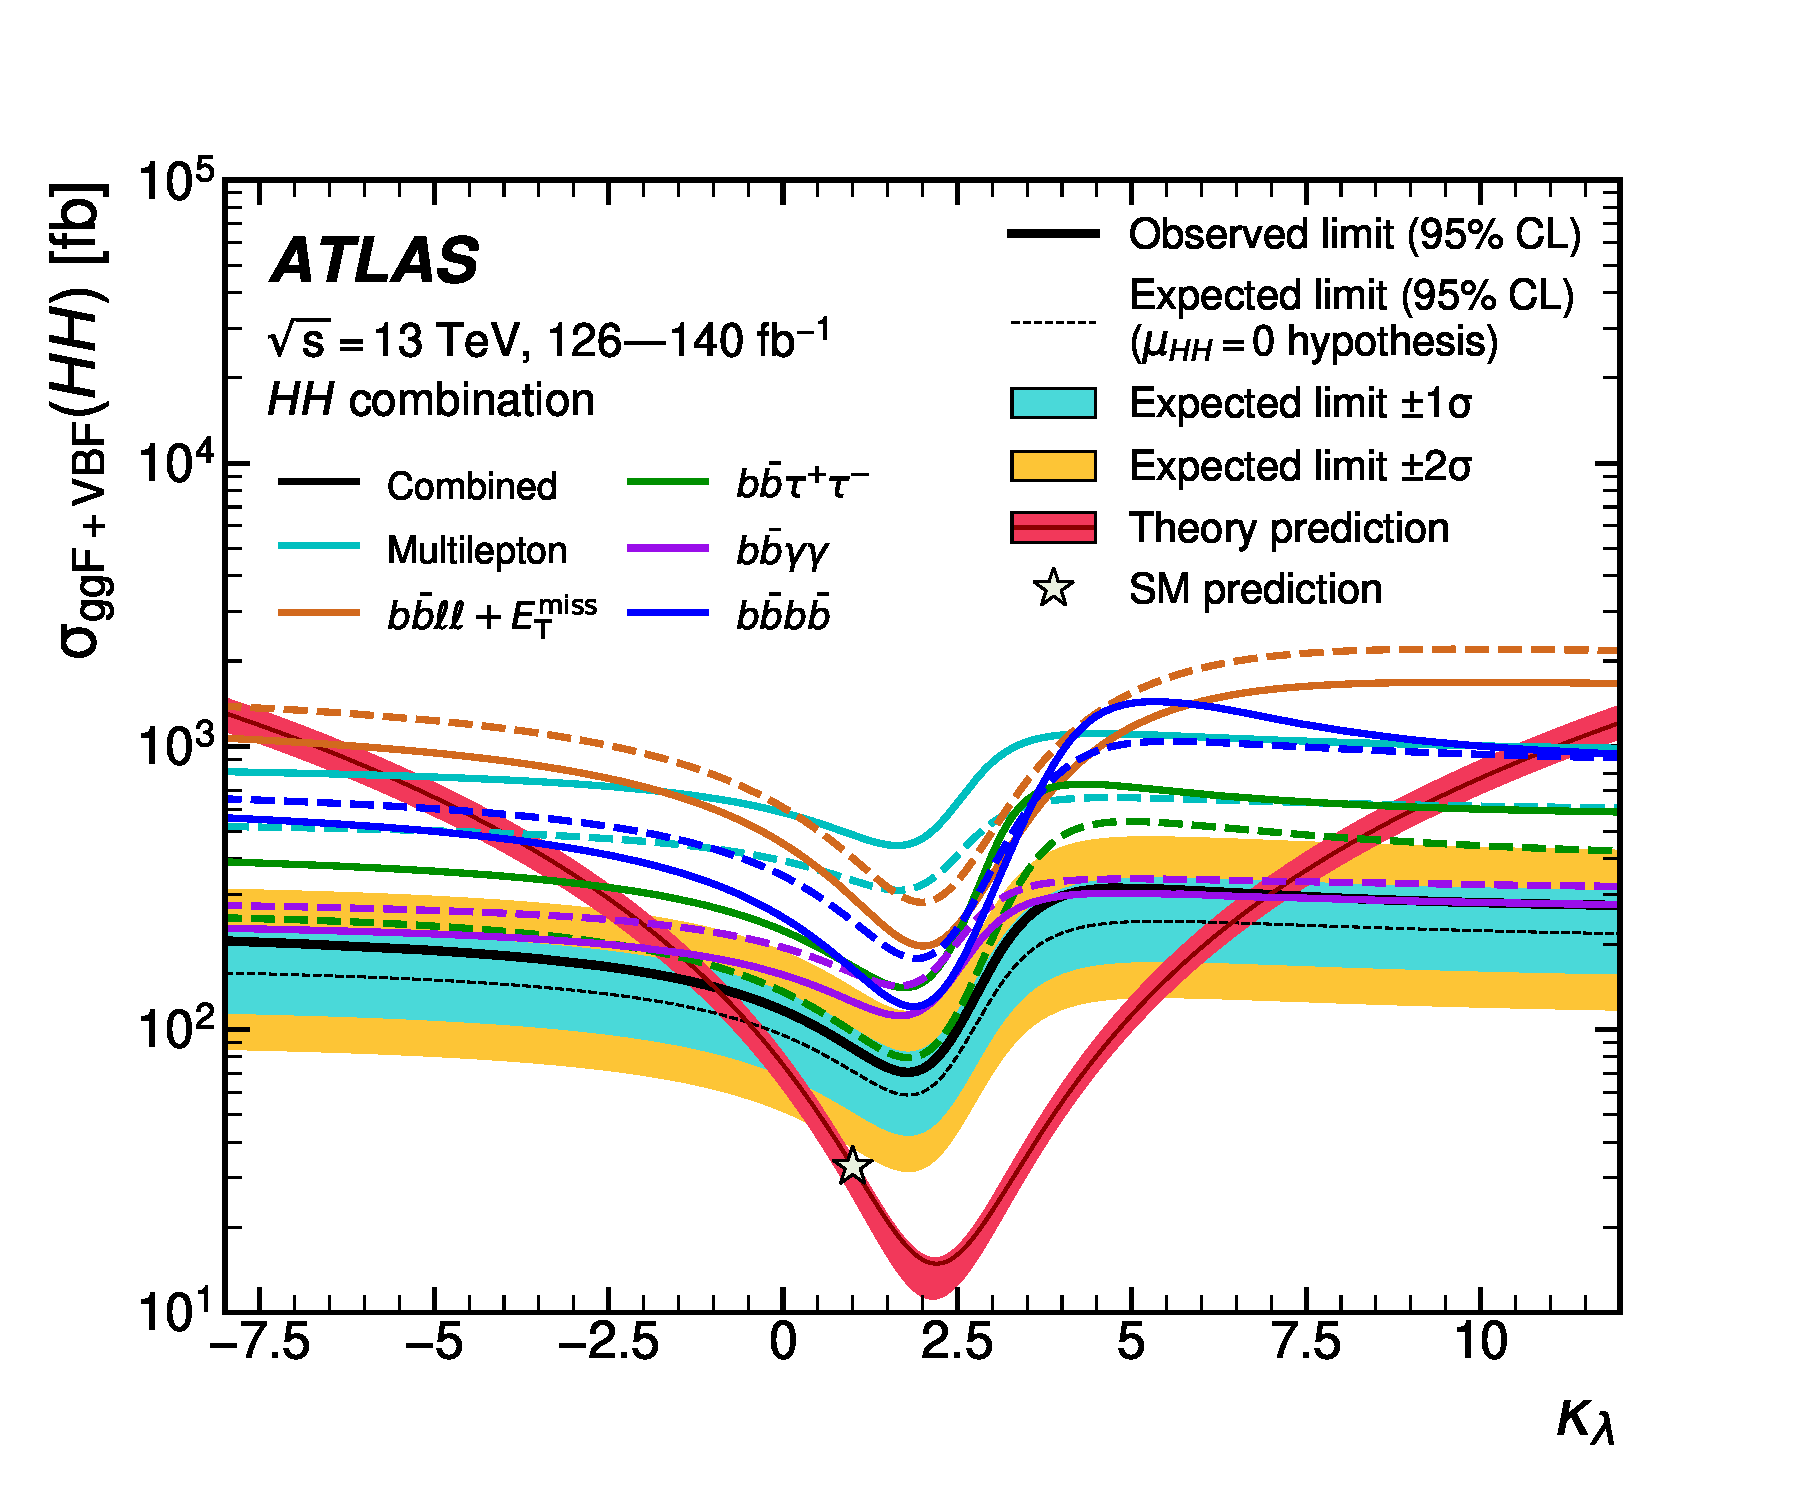
\includegraphics[width=.5\textwidth]{/home/bruno/org/PhD/Thesis/figures/intro/atlas_combination_kl.pdf}
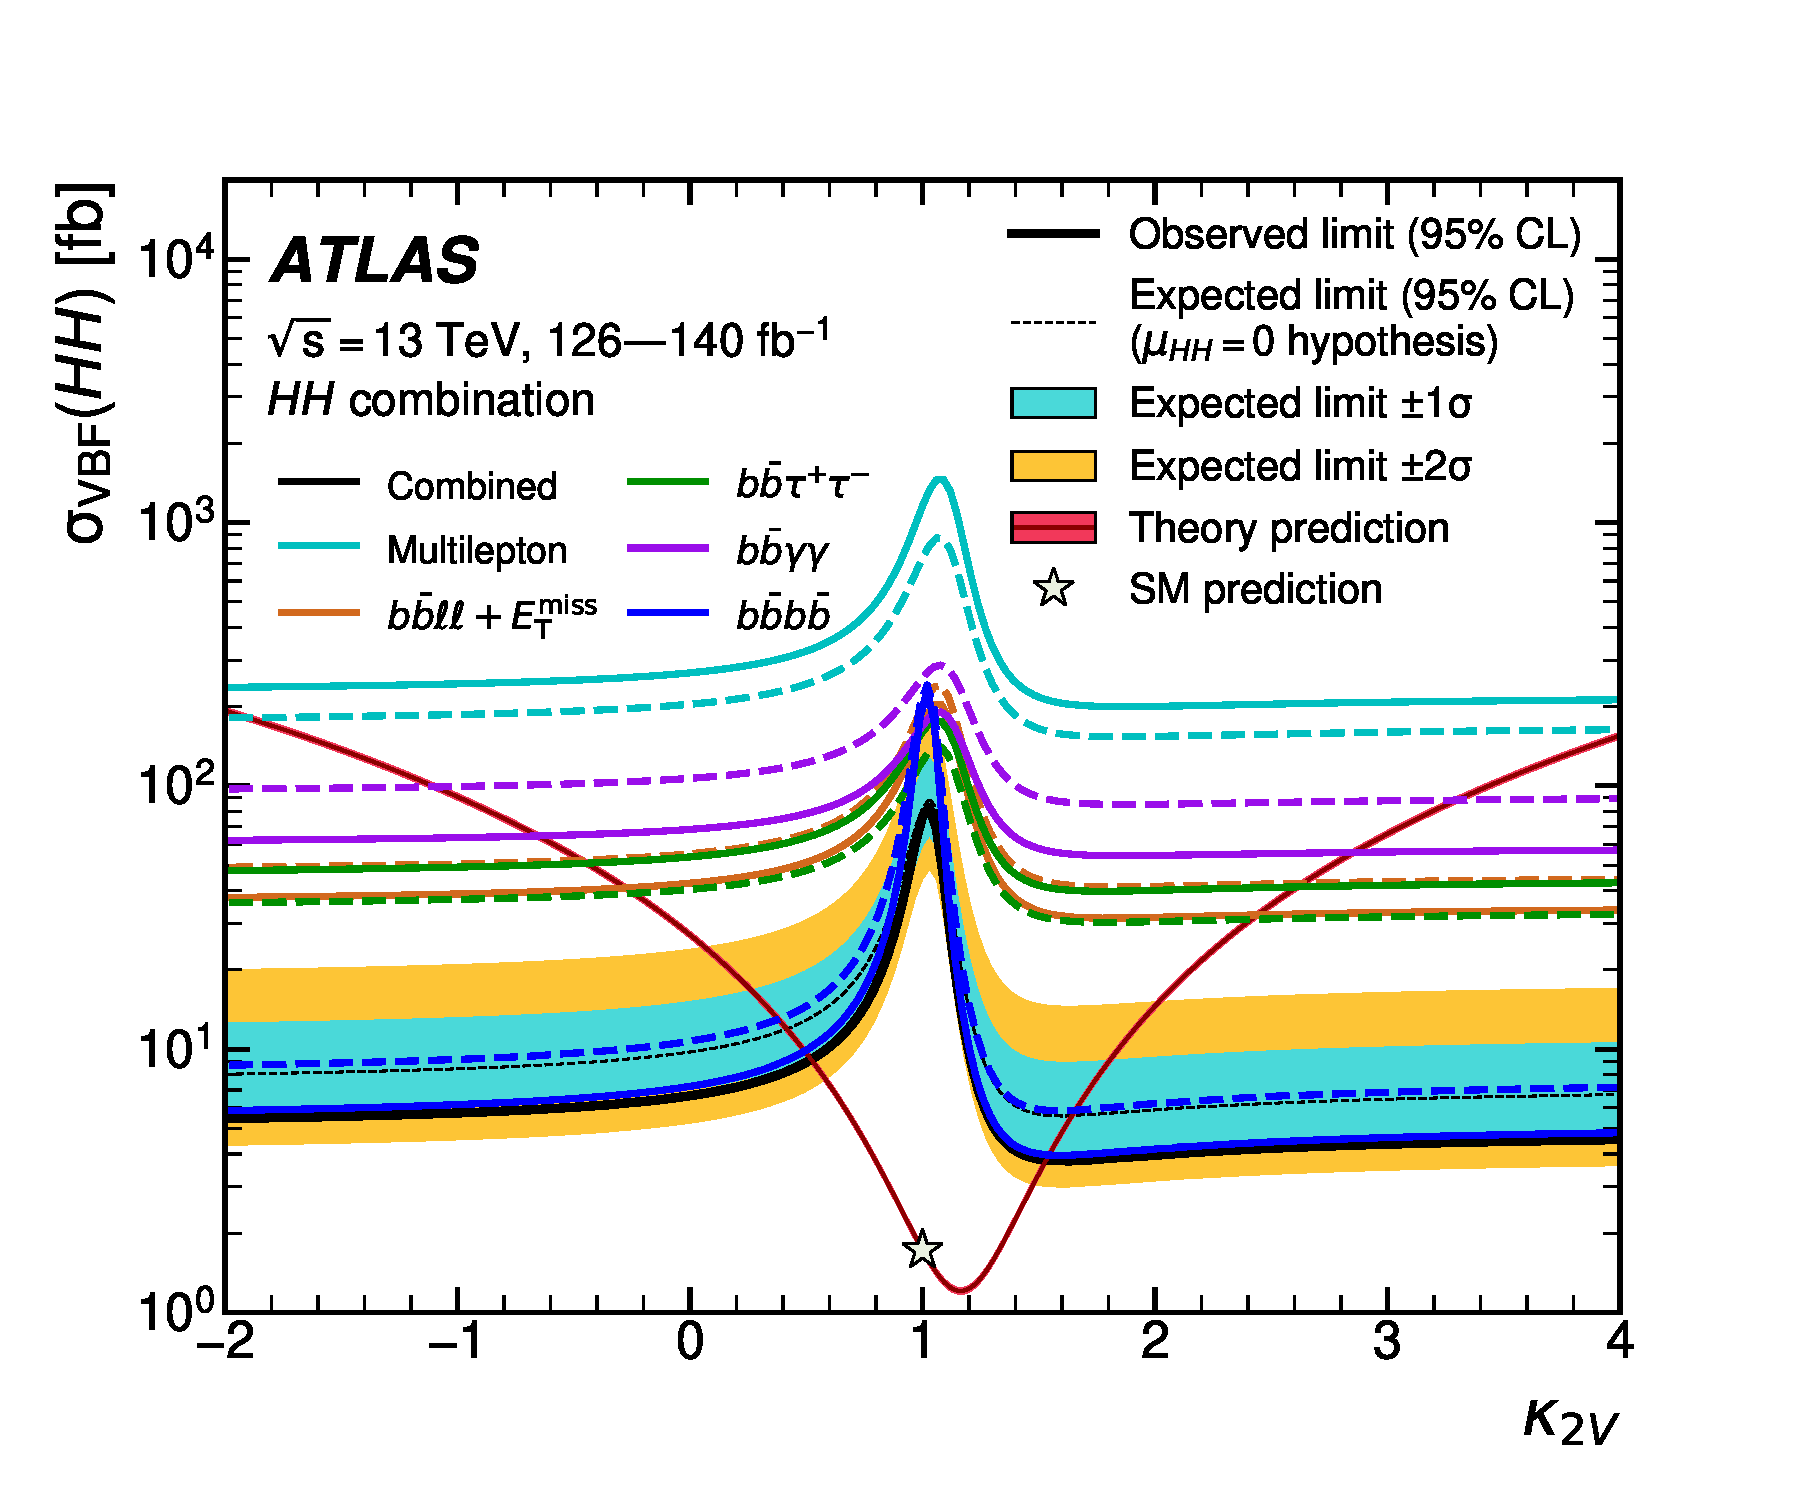
\includegraphics[width=.5\textwidth]{/home/bruno/org/PhD/Thesis/figures/intro/atlas_combination_k2v.pdf}
\caption{\label{fig:scan_comb_atlas}Observed (solid lines) and expected (dashed lines) 95\% CL exclusion limits on the HH production cross-sections of the inclusive \ac{ggF} and \ac{VBF} processes as a function of \(\kl\) (left) and the \ac{VBF} process as a function of \(\kvv\) (right), for the \bbgg{} (purple), \bbtt{} (green), multilepton (cyan), \bbbb{} (blue) and \bbll{} (brown) decay channels and their combination (black). The expected limits assume no HH production or no \ac{VBF} HH production, respectively. The \ac{ggF} HH production cross-section is assumed to be as predicted by the SM in the right plot. The red line shows the theory prediction for the \ac{ggF} and \ac{VBF} HH production cross-section as a function of \(\kl\) (left), and the predicted \ac{VBF} HH cross-section as a function of \(\kvv\) (right). The bands surrounding the red cross-section lines indicate the theoretical uncertainties on the predicted cross-sections. Taken from \cite{atlas_hh_comb}.}
\end{figure}


\begin{figure}
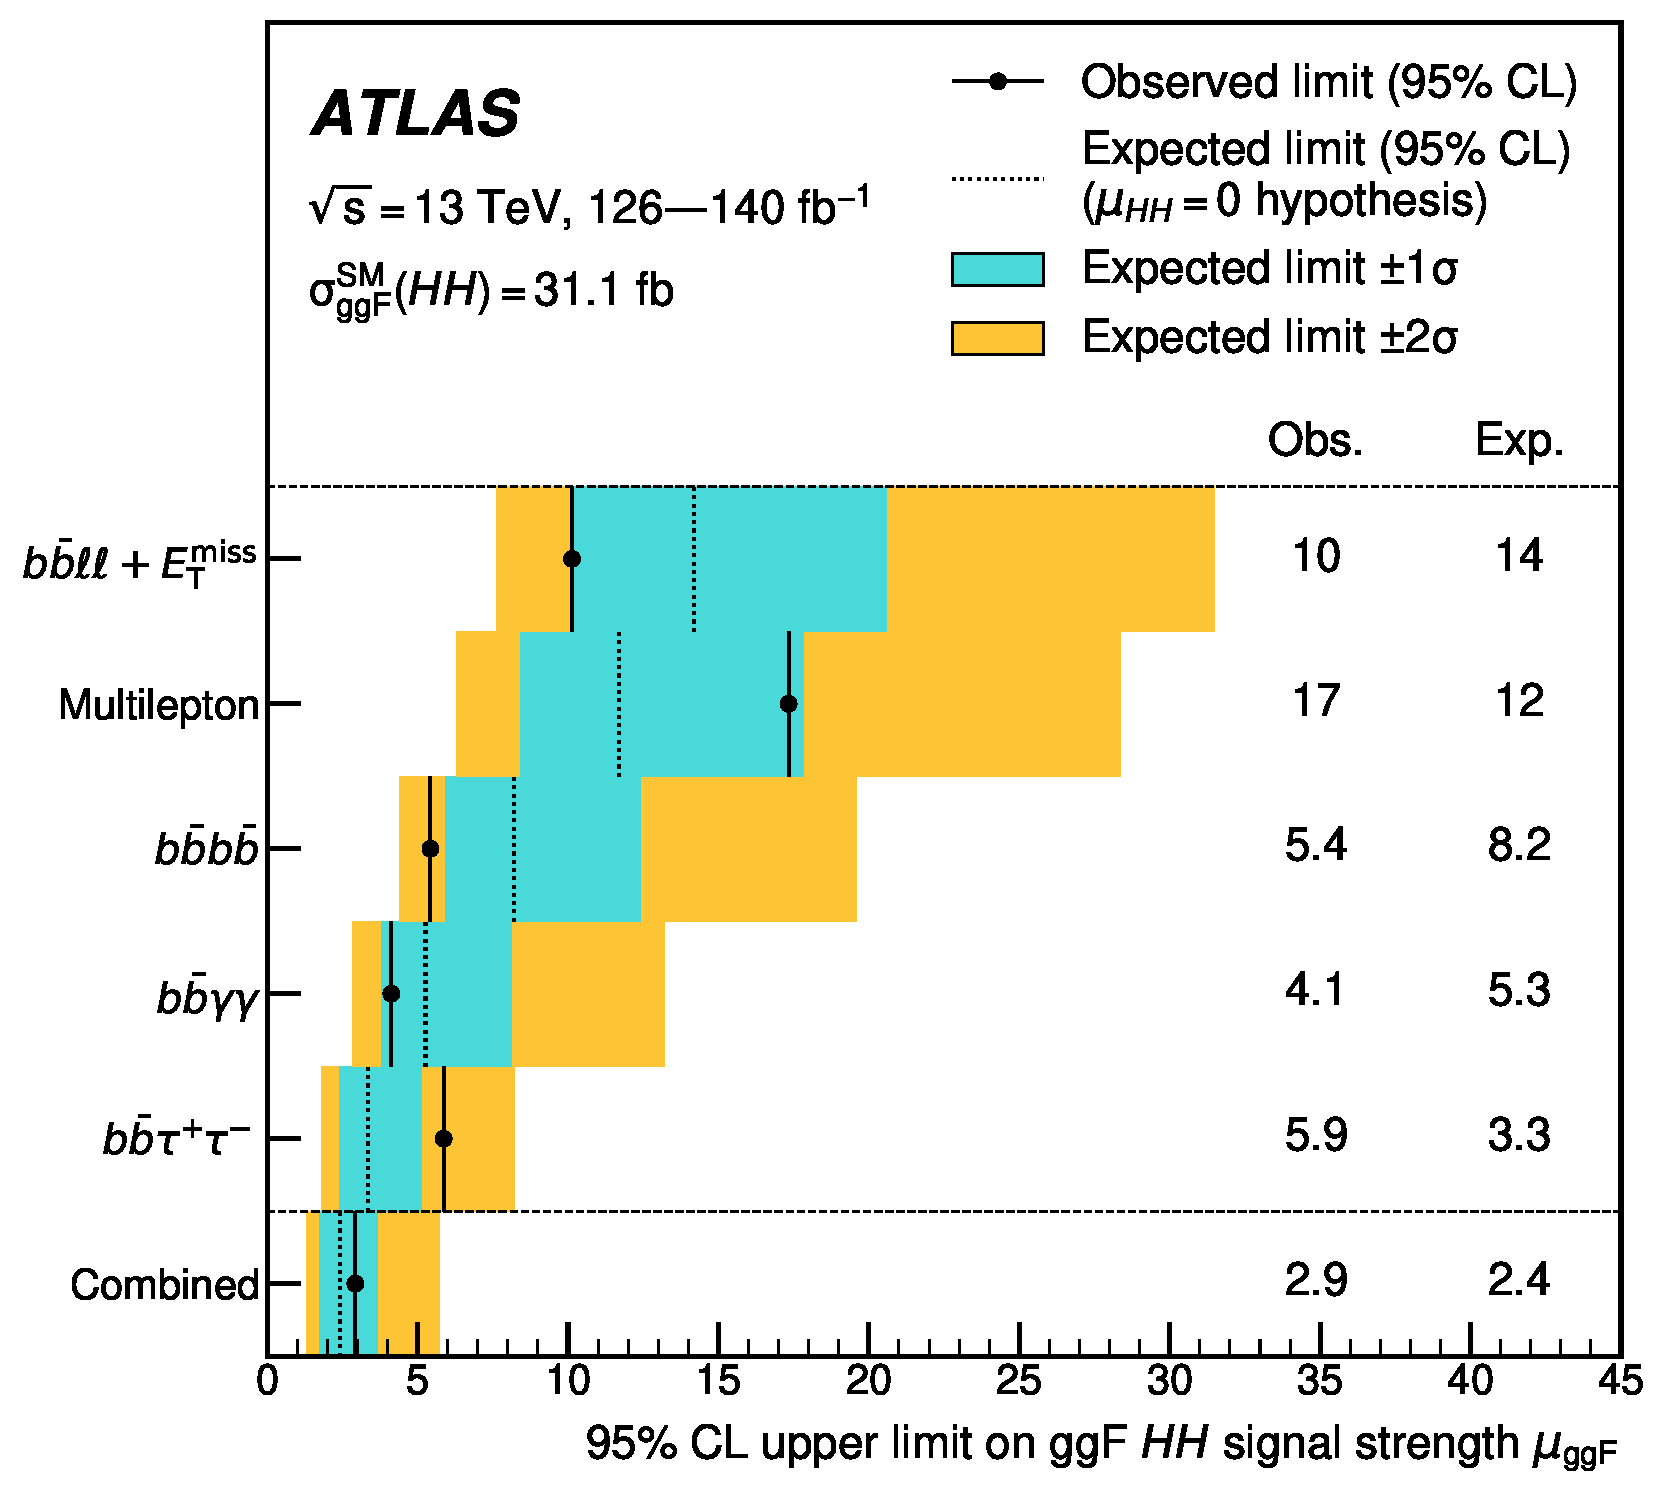
\includegraphics[width=.5\textwidth]{/home/bruno/org/PhD/Thesis/figures/intro/limits_ggF_HH_SM_atlas.pdf}
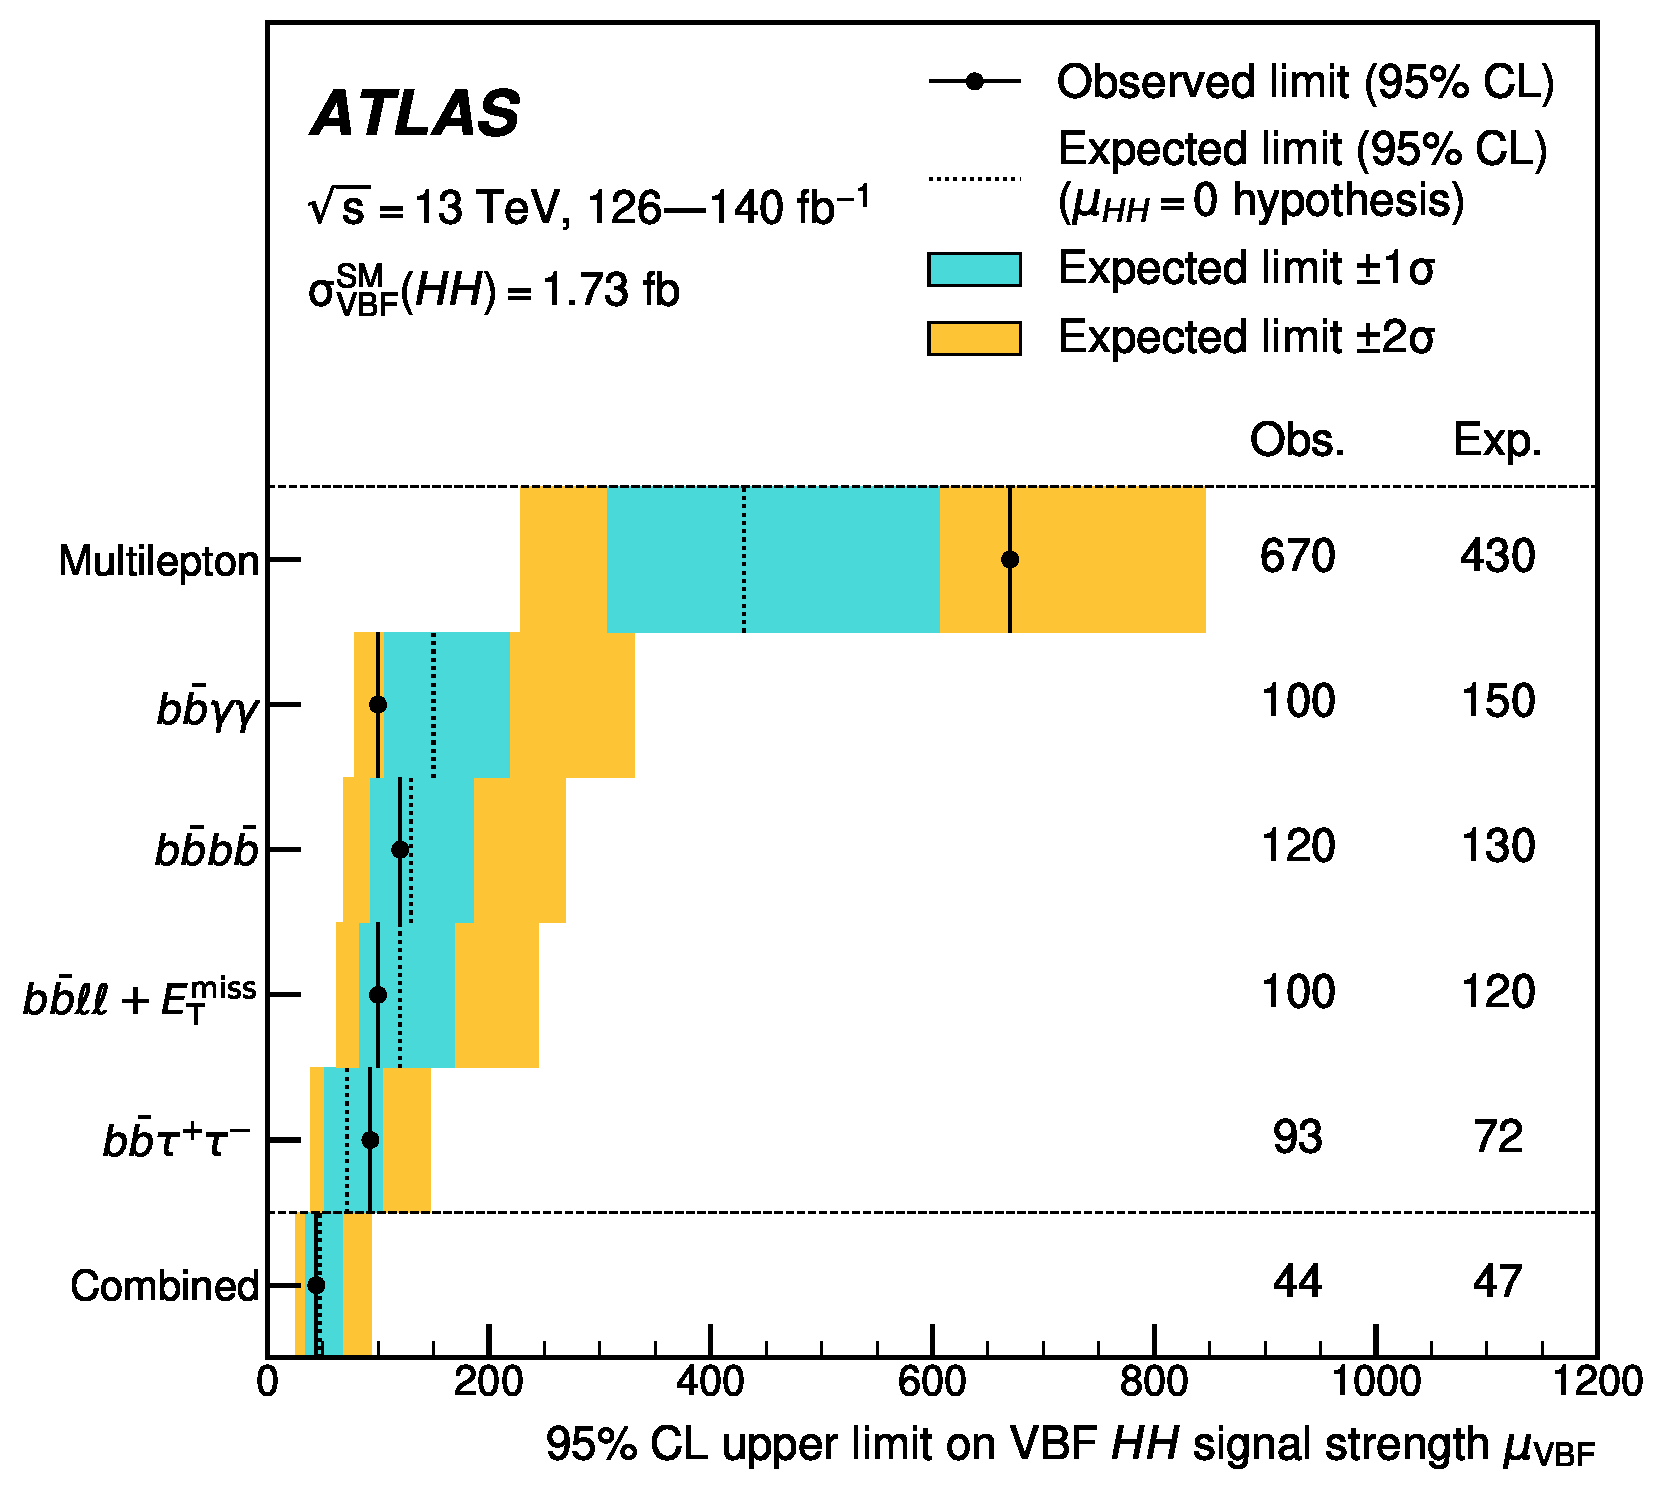
\includegraphics[width=.5\textwidth]{/home/bruno/org/PhD/Thesis/figures/intro/limits_VBF_HH_SM_atlas.pdf}
\caption{\label{fig:limits_comb_atlas}Observed and expected 95\% CL upper limits on the signal strength for the inclusive \ac{ggF} HH (left) and \ac{VBF} HH production (right) from the \bbtt{}, \bbgg{}, \bbbb{}, multilepton and \bbll{} decay channels, and their statistical combination. The \ac{ggF} or \ac{VBF} HH production cross-section is fixed to the SM predicted value for \(\mh=125\,\si{\GeV}\) when deriving limits on the respective signal strength. The expected limit, along with the ±1σ and ±2σ bands, is calculated under the assumption of no HH process and with all NPs profiled to the observed data. Taken from \cite{atlas_hh_comb}.}
\end{figure}

\begin{figure}
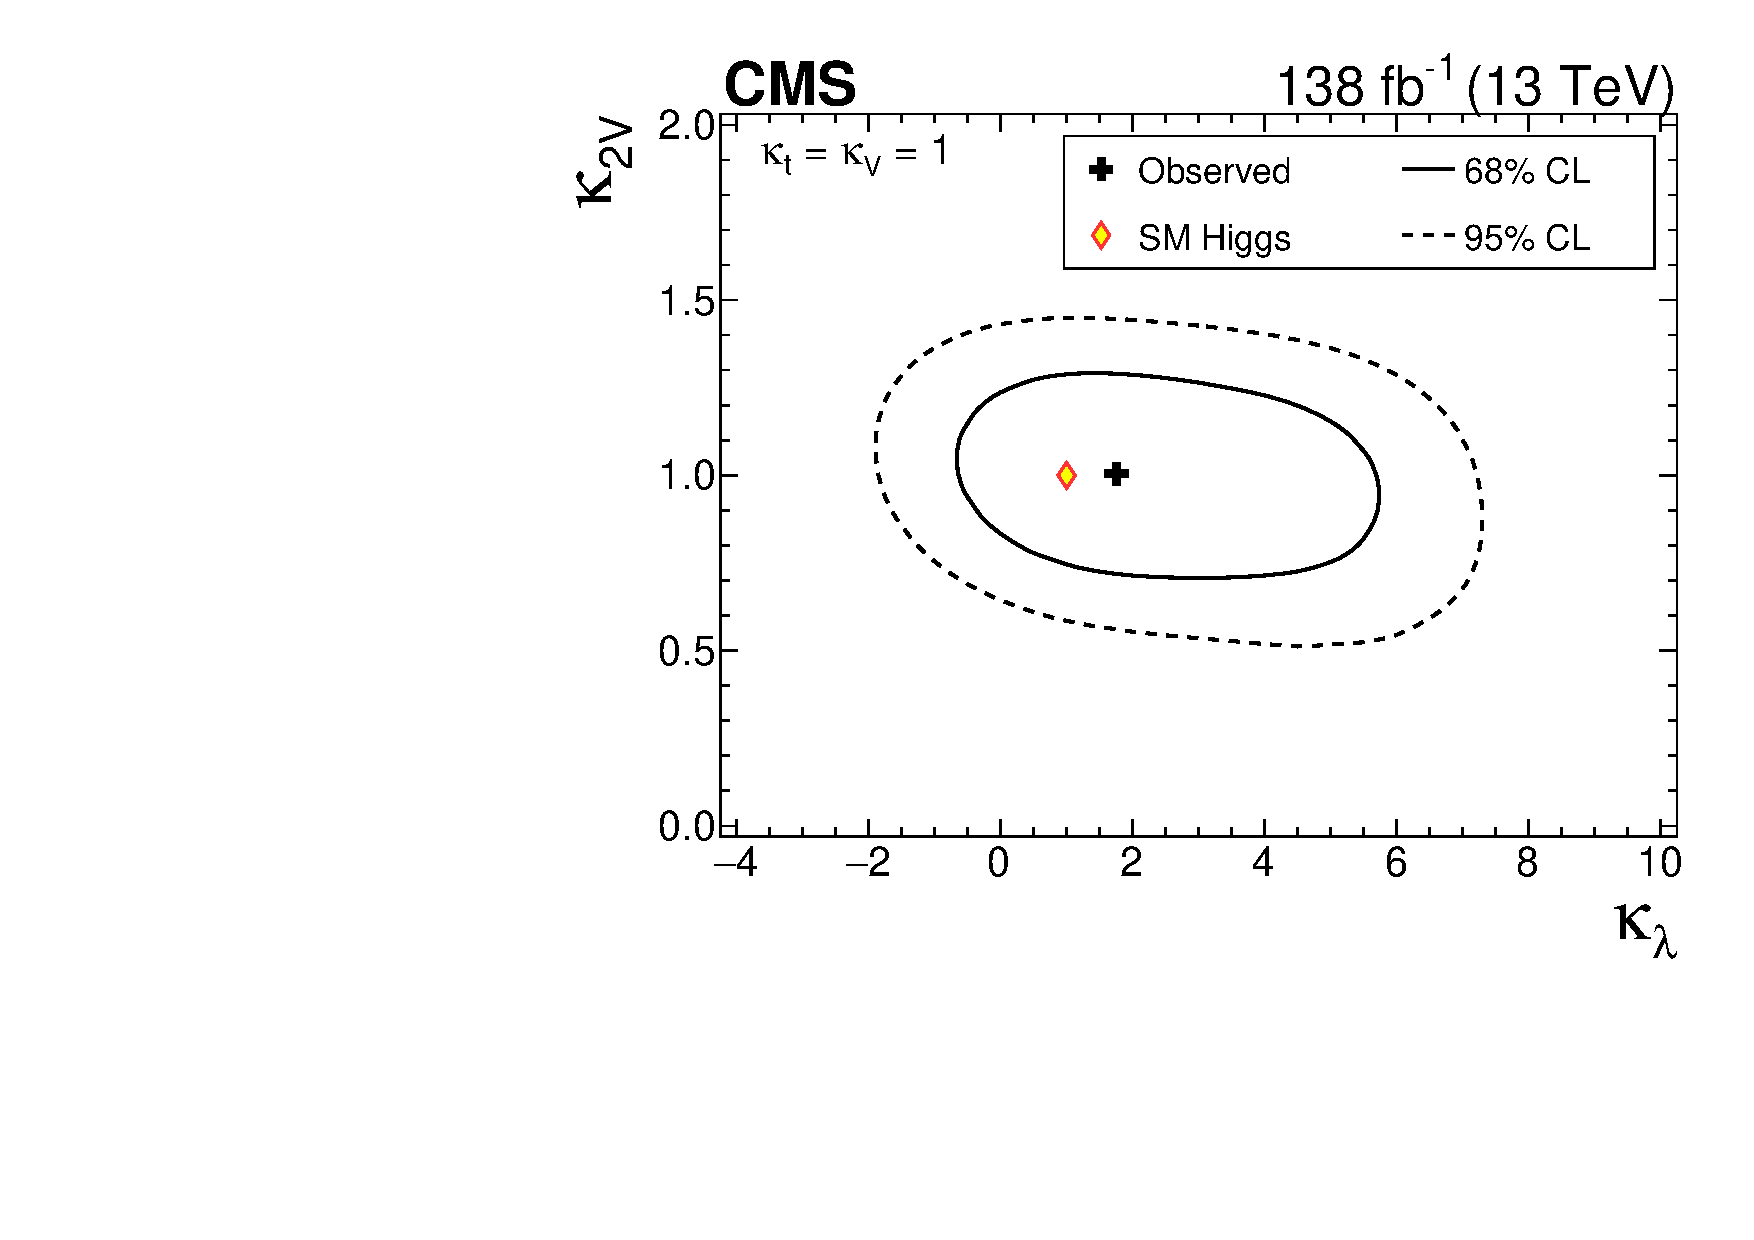
\includegraphics[width=.431\textwidth]{/home/bruno/org/PhD/Thesis/figures/intro/direct_indirect1.pdf}
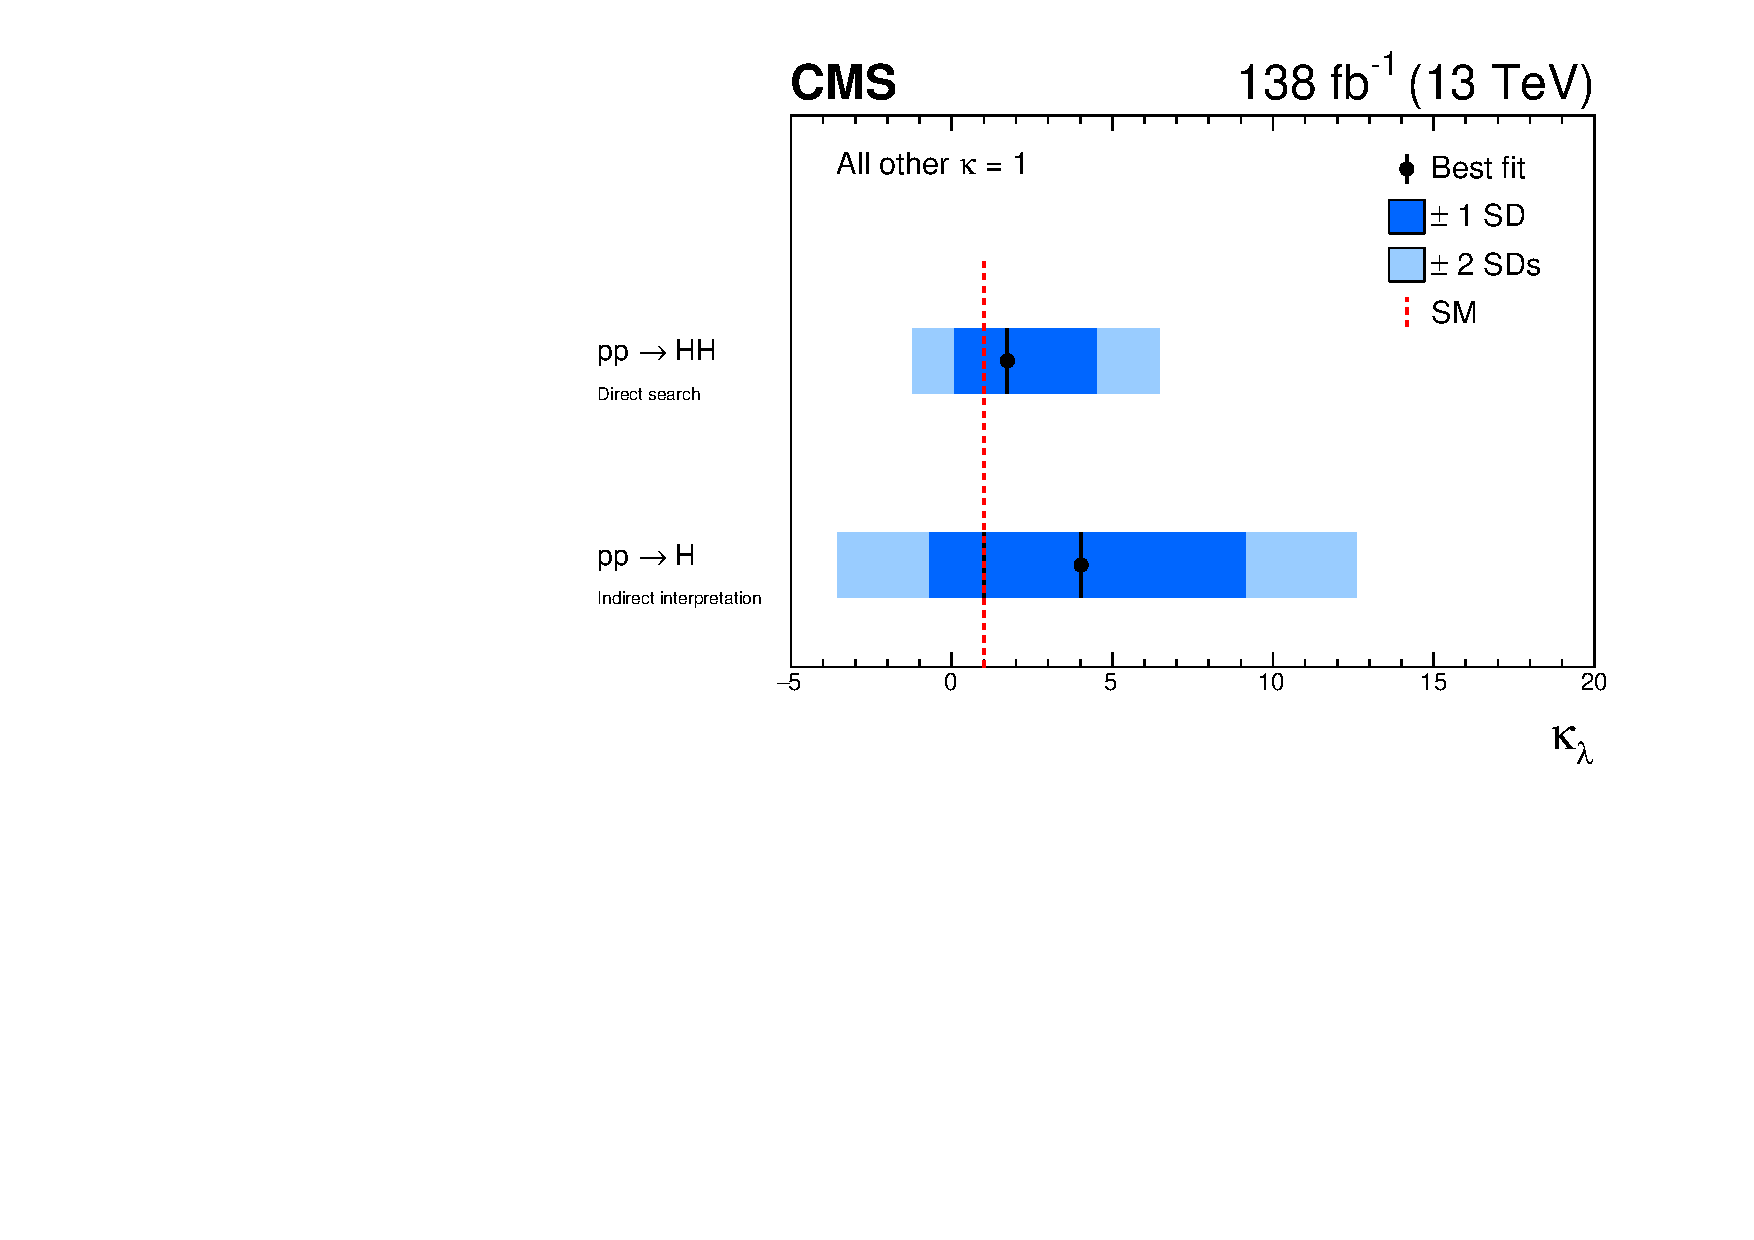
\includegraphics[width=.569\textwidth]{/home/bruno/org/PhD/Thesis/figures/intro/direct_indirect2.pdf}
\caption{\label{fig:direct_vs_indirect_cms}Constraints on \(\kl\) and \(\kvv\) from the production of Higgs boson pairs (left). Constraint on the Higgs boson self-coupling modifier \(\kl\) from single and pair production of Higgs boson(s) (right). Taken from \cite{higgs_10_years}.}
\end{figure}

\begin{figure}
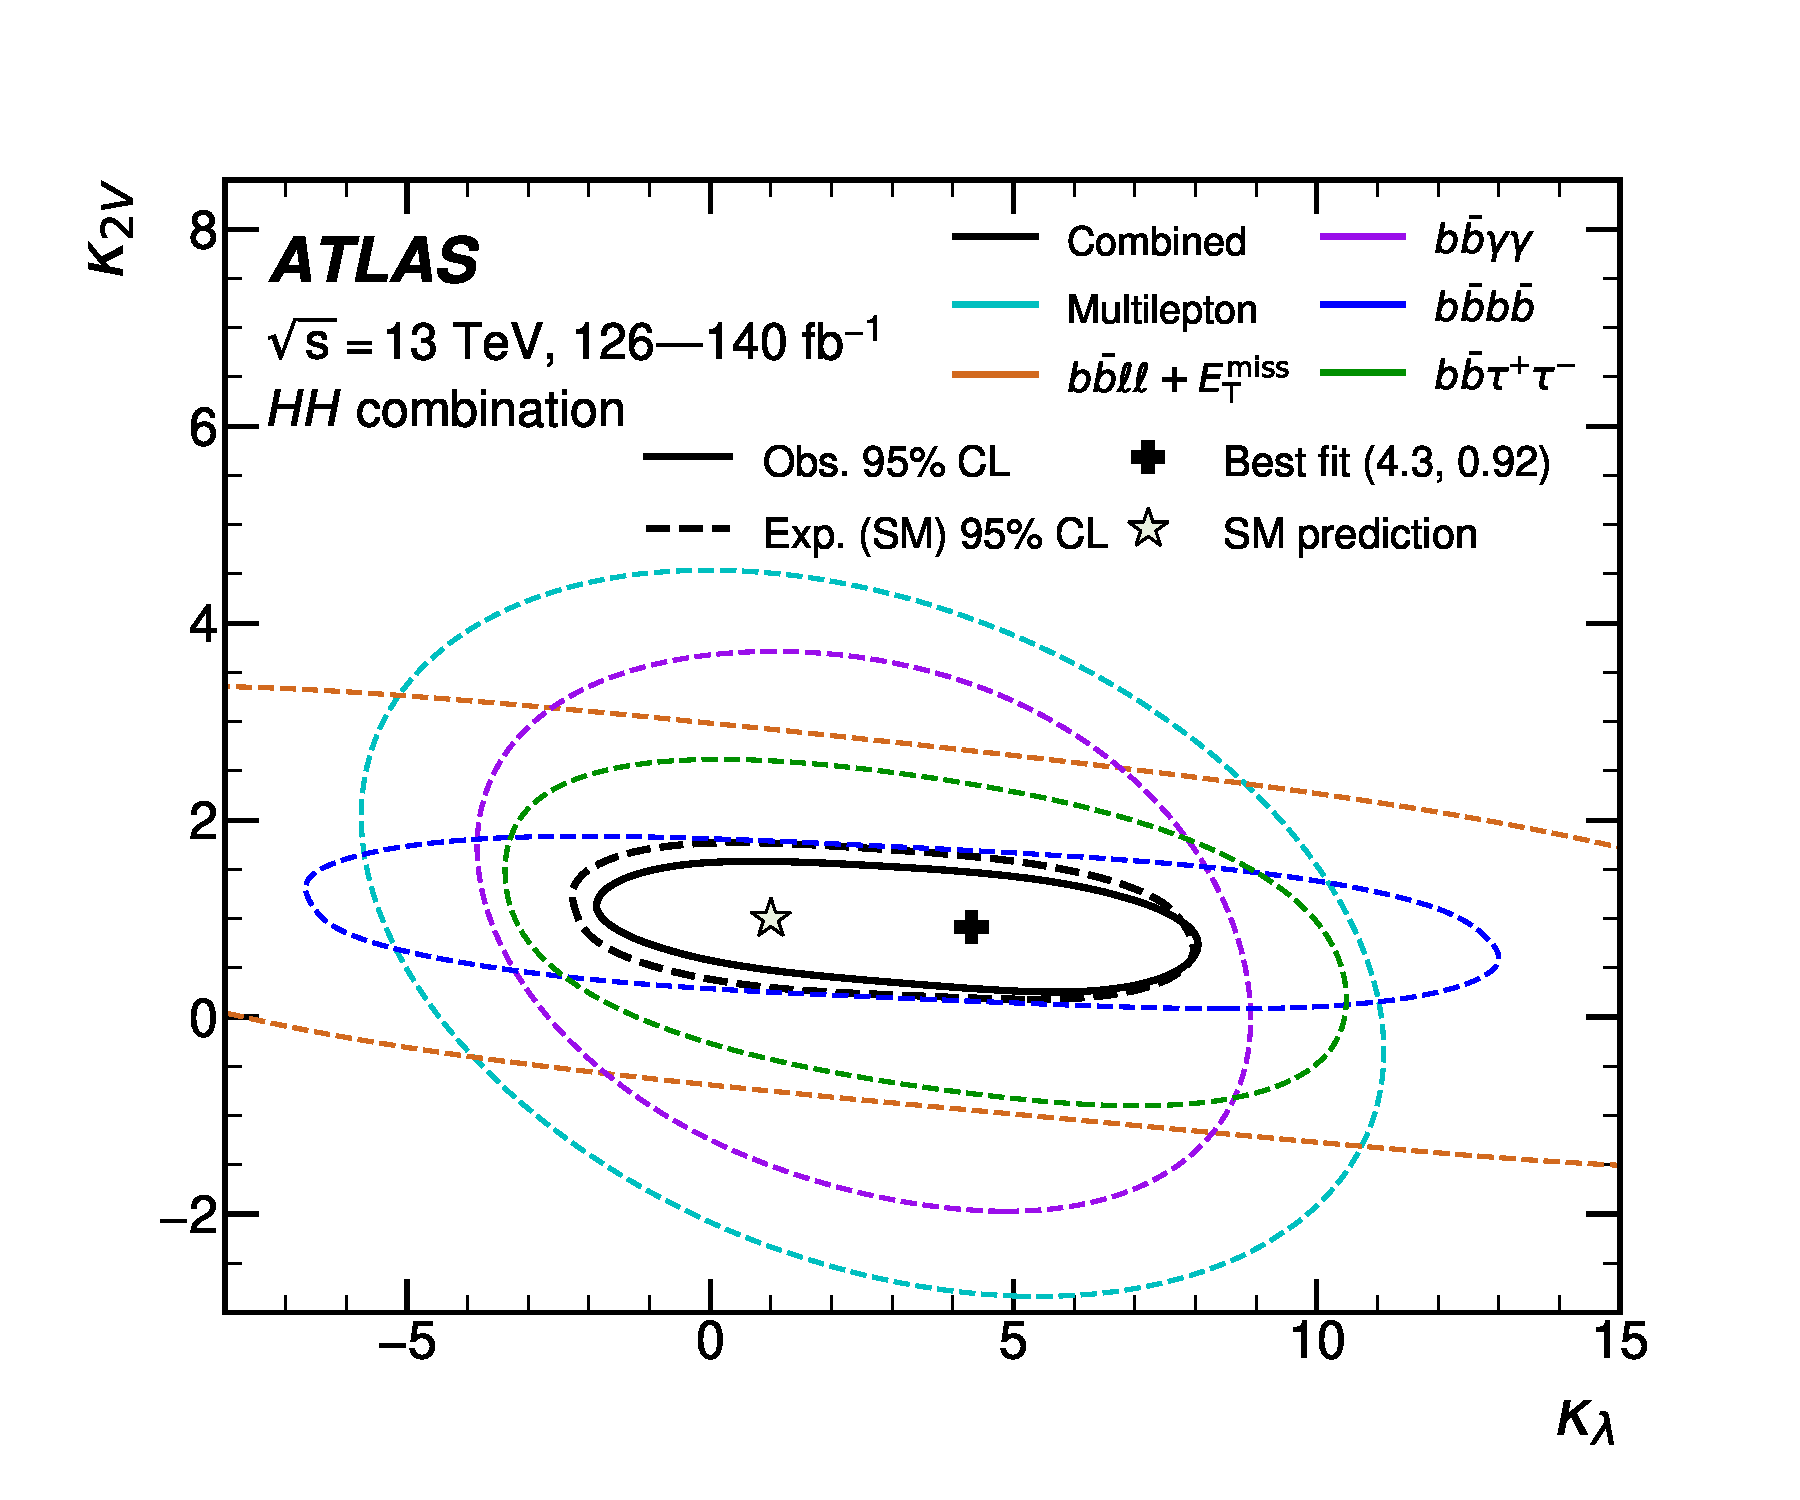
\includegraphics[width=.5\textwidth]{/home/bruno/org/PhD/Thesis/figures/intro/kl_vs_k2v_atlas_comb.pdf}
\caption{\label{fig:kl_vs_k2v_atlas}Expected 95\% CL contours in the \(\kvv{}–kl{}\) plane, corresponding to the individual decay channels and their combination, are illustrated using dashed lines. The observed contour from the combined results is depicted by a solid black line. The \ac{SM} prediction is marked by a star, and the combined best-fit value is indicated by a cross. Taken from \cite{atlas_hh_comb}.}
\end{figure}

\begin{figure}
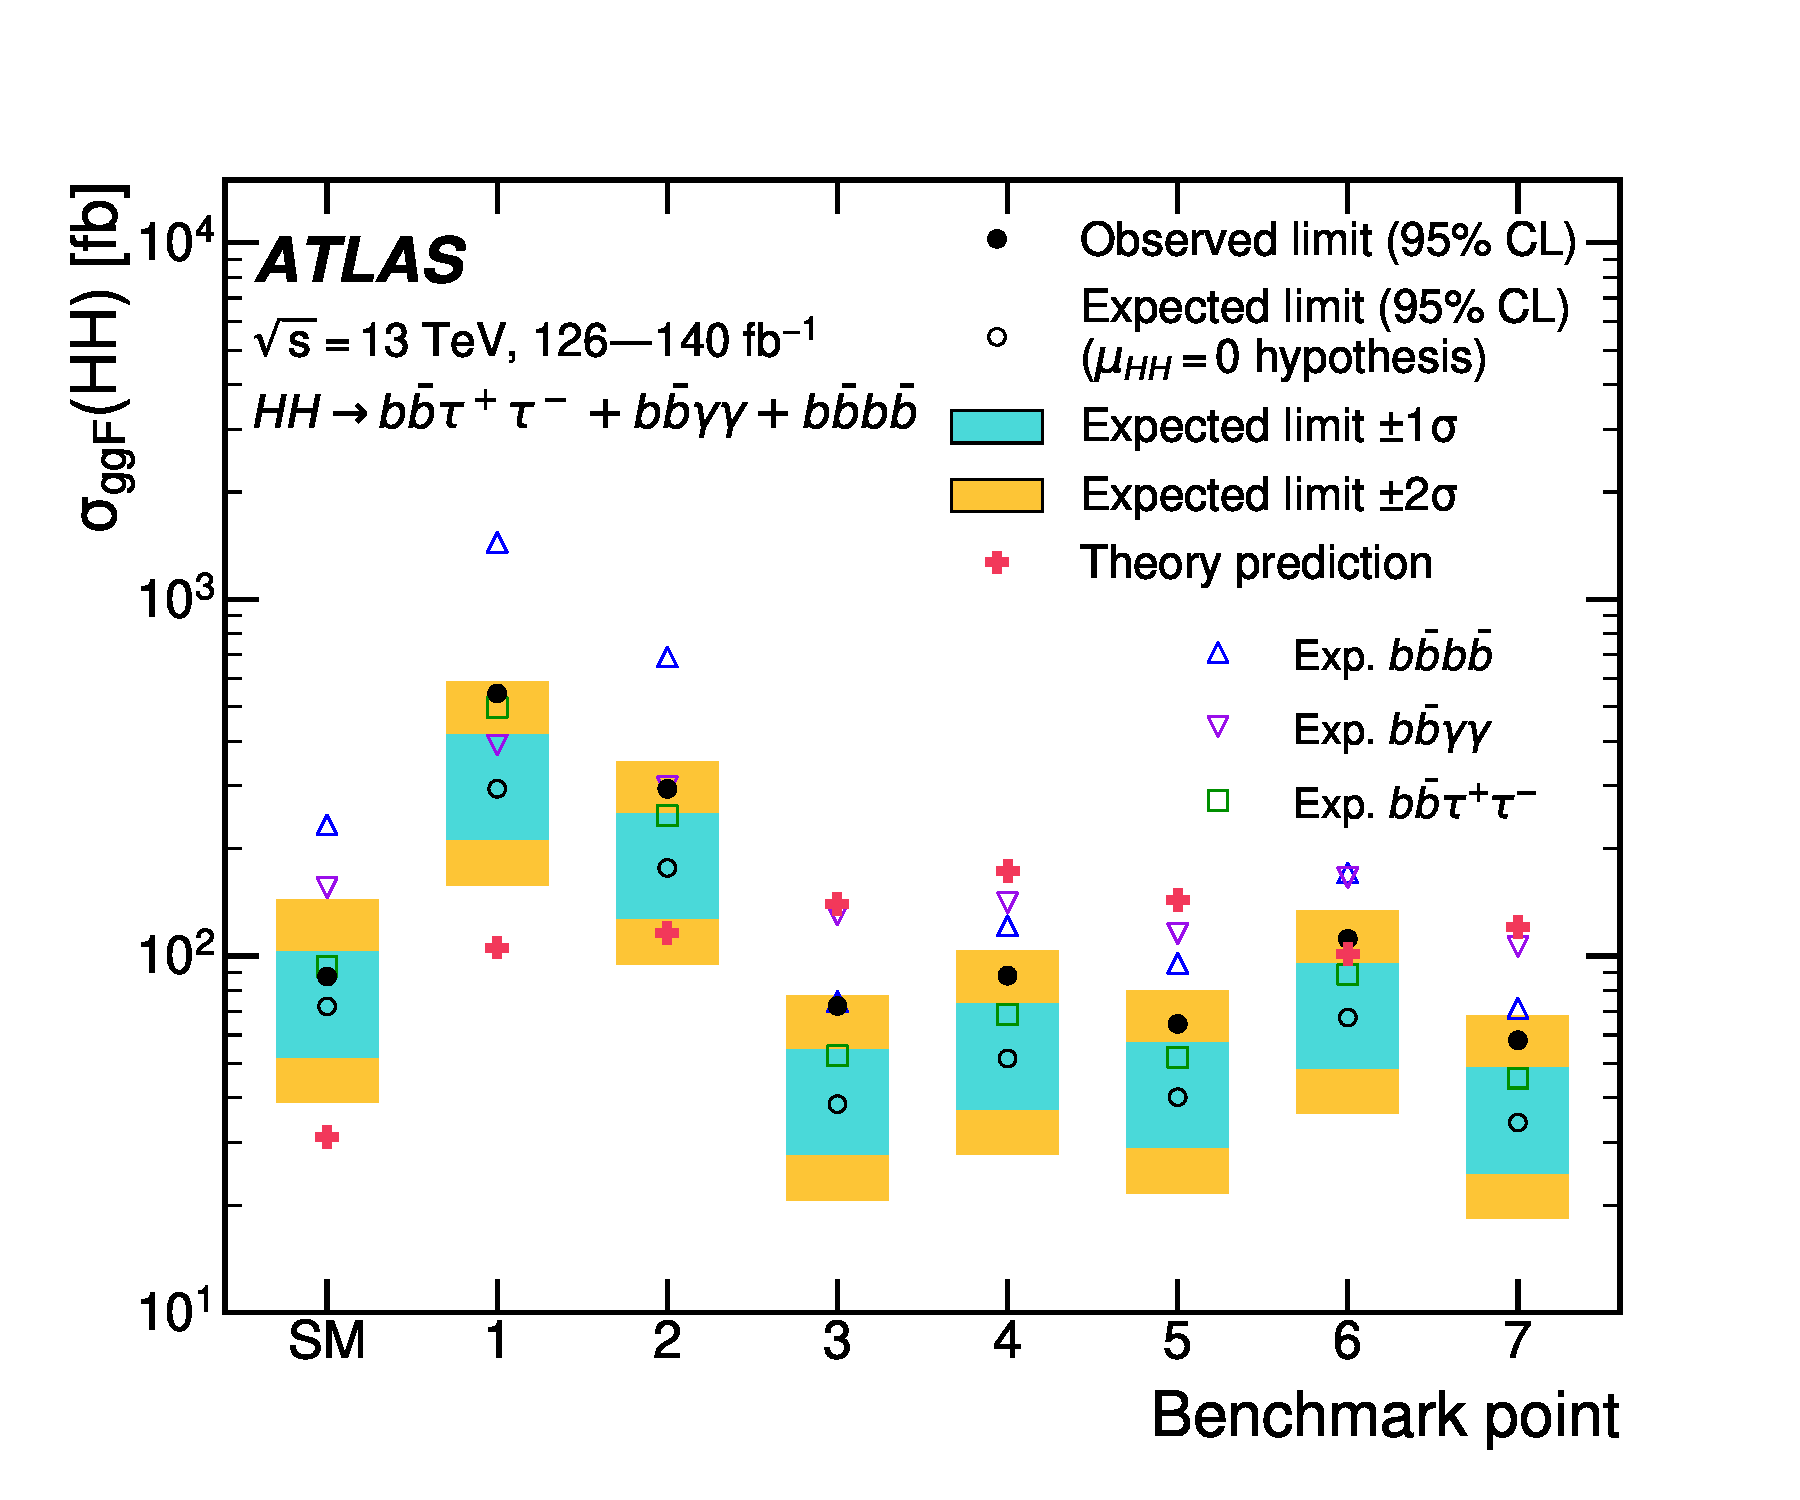
\includegraphics[width=.5\textwidth]{/home/bruno/org/PhD/Thesis/figures/intro/eft_atlas_comb.pdf}
\caption{\label{fig:kl_vs_k2v_atlas}Observed and expected 95\% CL combined upper limits on the cross-section for the \ac{SM} and seven \ac{BSM} HEFT benchmarks in the ggF process, describing representative signal kinematics and \(\mhh\) shape features obtained by varying multiple \ac{HEFT} coefficients. The expected limits from the \bbtt{}, \bbgg{} and \bbbb{} decay channels are presented as well. Theoretical predictions, estimated using specific sets of coefficient values defined in the benchmarks, are shown as red cross dots. Taken from \cite{atlas_hh_comb}.}
\end{figure}



On top of the HH searches already mentioned, \(\kl\) can be additionally constrained by exploiting \ac{NLO} \ac{EW} corrections to single Higgs processes, which also depend on \(\kl\).
Single Higgs cross-sections can indeed be quite sensitive to \(\kl\) variations, especially in the \vh{} and \tth{} production modes, where up to 10\% differences are expected.
Additionally, there is a strong complementarity between direct and indirect searches \cite{indirect_searches2}.
HH searches generally provide weaker contraints on the Higgs boson coupling to fermions and vector bosons, due to the lower production cross-section with respect to single Higgs.
On the other hand, double Higgs processes provide stronger constraints on \(\kl\).

The main challenge of the combination recently performed by \ac{CMS} \cite{CMSHplusHHcomb} consists on estimating and efficiently removing overlaps between signal regions of different analysis.
The mitigation of double-counting and minimization of overlaps, together with the combination of event categories from both single and double-Higgs analysis, lead to stronger \(\kl\) constraints.
The analysis with the most sensitive production modes are included.
Whenever overlaps exist, one of two approaches is taken: either additional selections are applied, or the least sensitive category or analysis is removed.
As an example, the \bbzz{} analysis is removed in favour of \zzfourl{} due to the former's relatively low sensitivity to \(\kl\).
Concerning systematics, their modelling in HH processes is generally simpler when compared to single H, due to the limited statistics of HH.

\ac{CMS} observed exclusion intervals at 95\% \ac{CL} of \(-0.4 < \kl < 6.3\), assuming other Higgs couplings to follow the \ac{SM}, or \(-1.4 < k_{\lambda} < 6.1\) otherwise.
For comparison, \ac{ATLAS} observed \(-0.4 < \kl < 6.3\), assuming \ac{SM} couplings, or \(-1.4 < k_{\lambda} < 6.1\) otherwise \cite{ATLASHplusHHcomb}.
We show (\(\kl\), \(\kt\)) and (\(\kv\), \(\kvv\)) scans in \cref{fig:combination_2d_scans}, where the complementarity between the two types of processes is clearly highlighted.
\ac{CMS} was also able to once again \cite{higgs_10_years} exclude \(\kvv=0\) at more than 5\(\sigma\), this time without fixing \(\kv=1\).

\begin{figure}
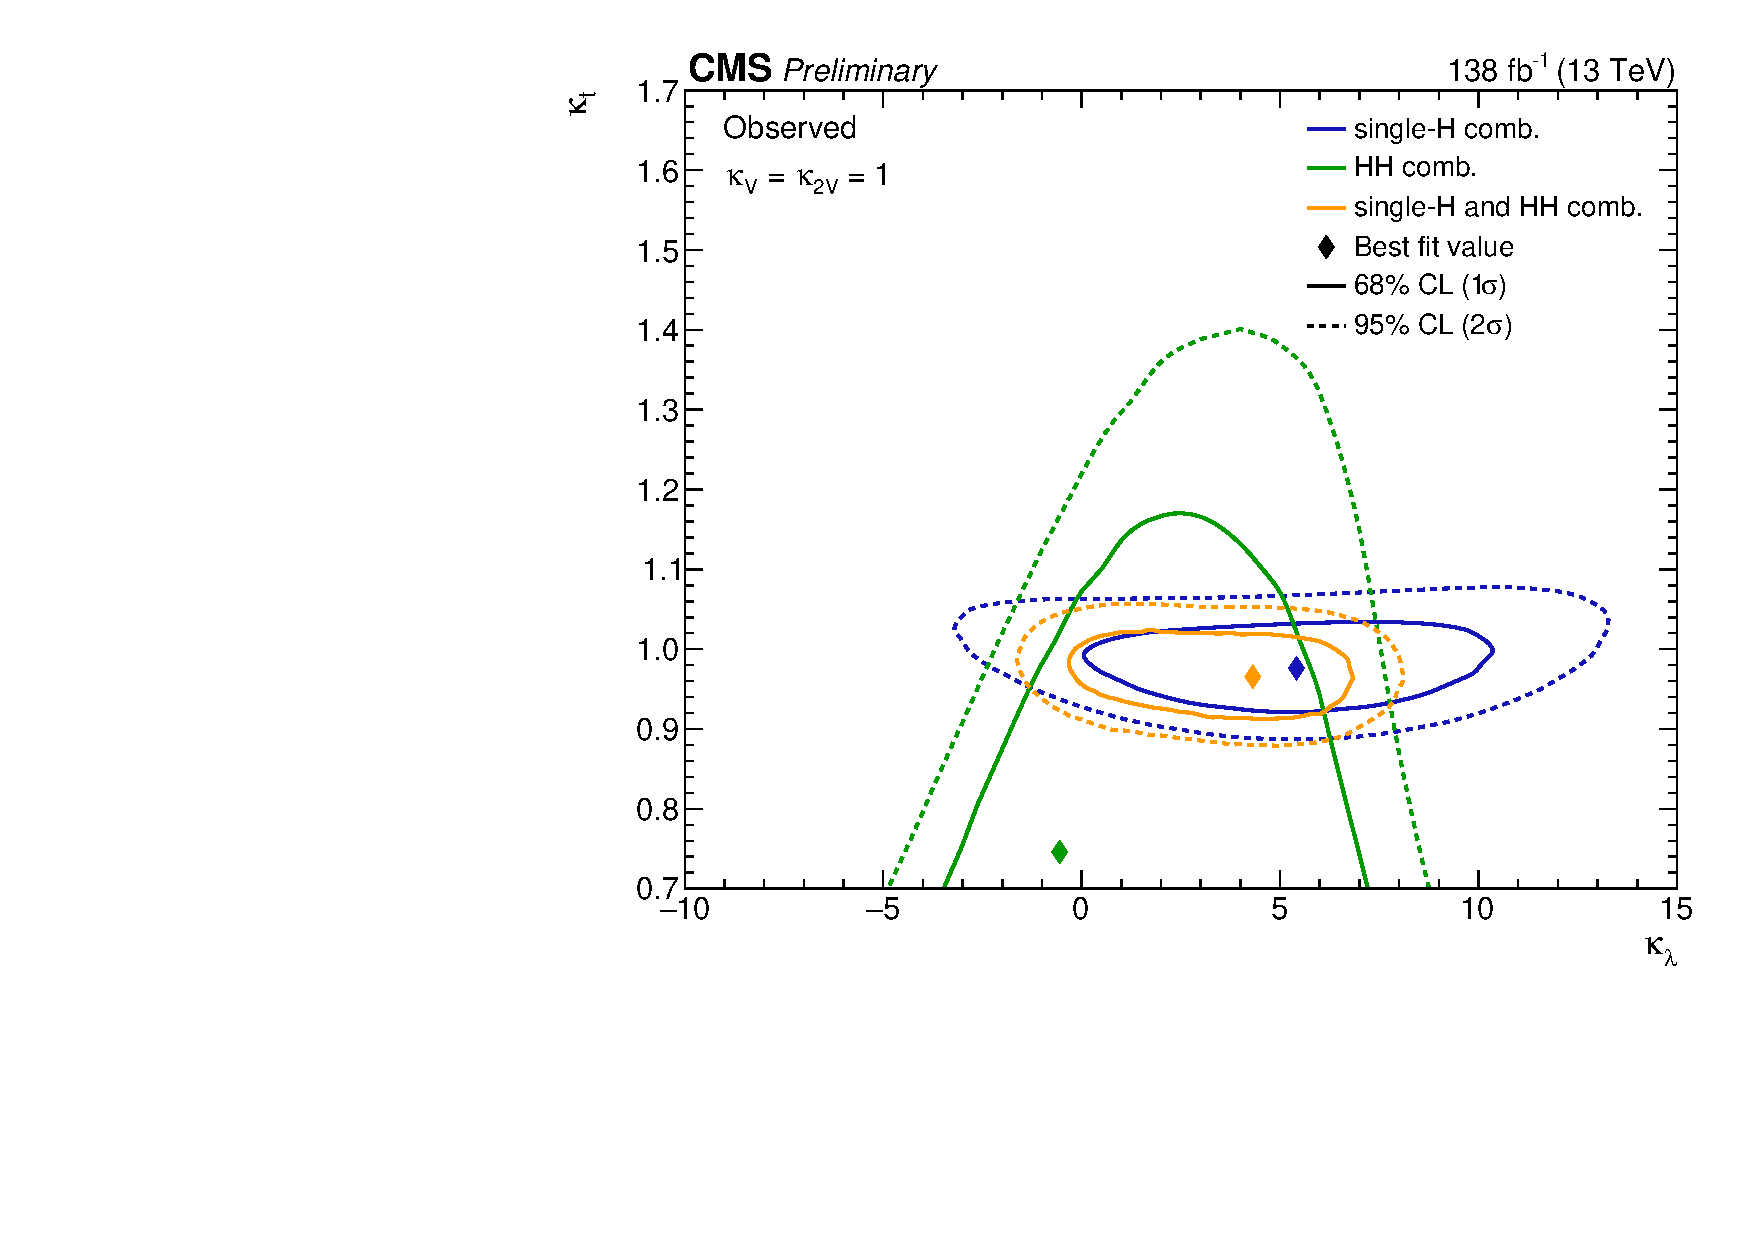
\includegraphics[width=.5\textwidth]{/home/bruno/org/PhD/Thesis/figures/combination_single_double_kl_kt.pdf}
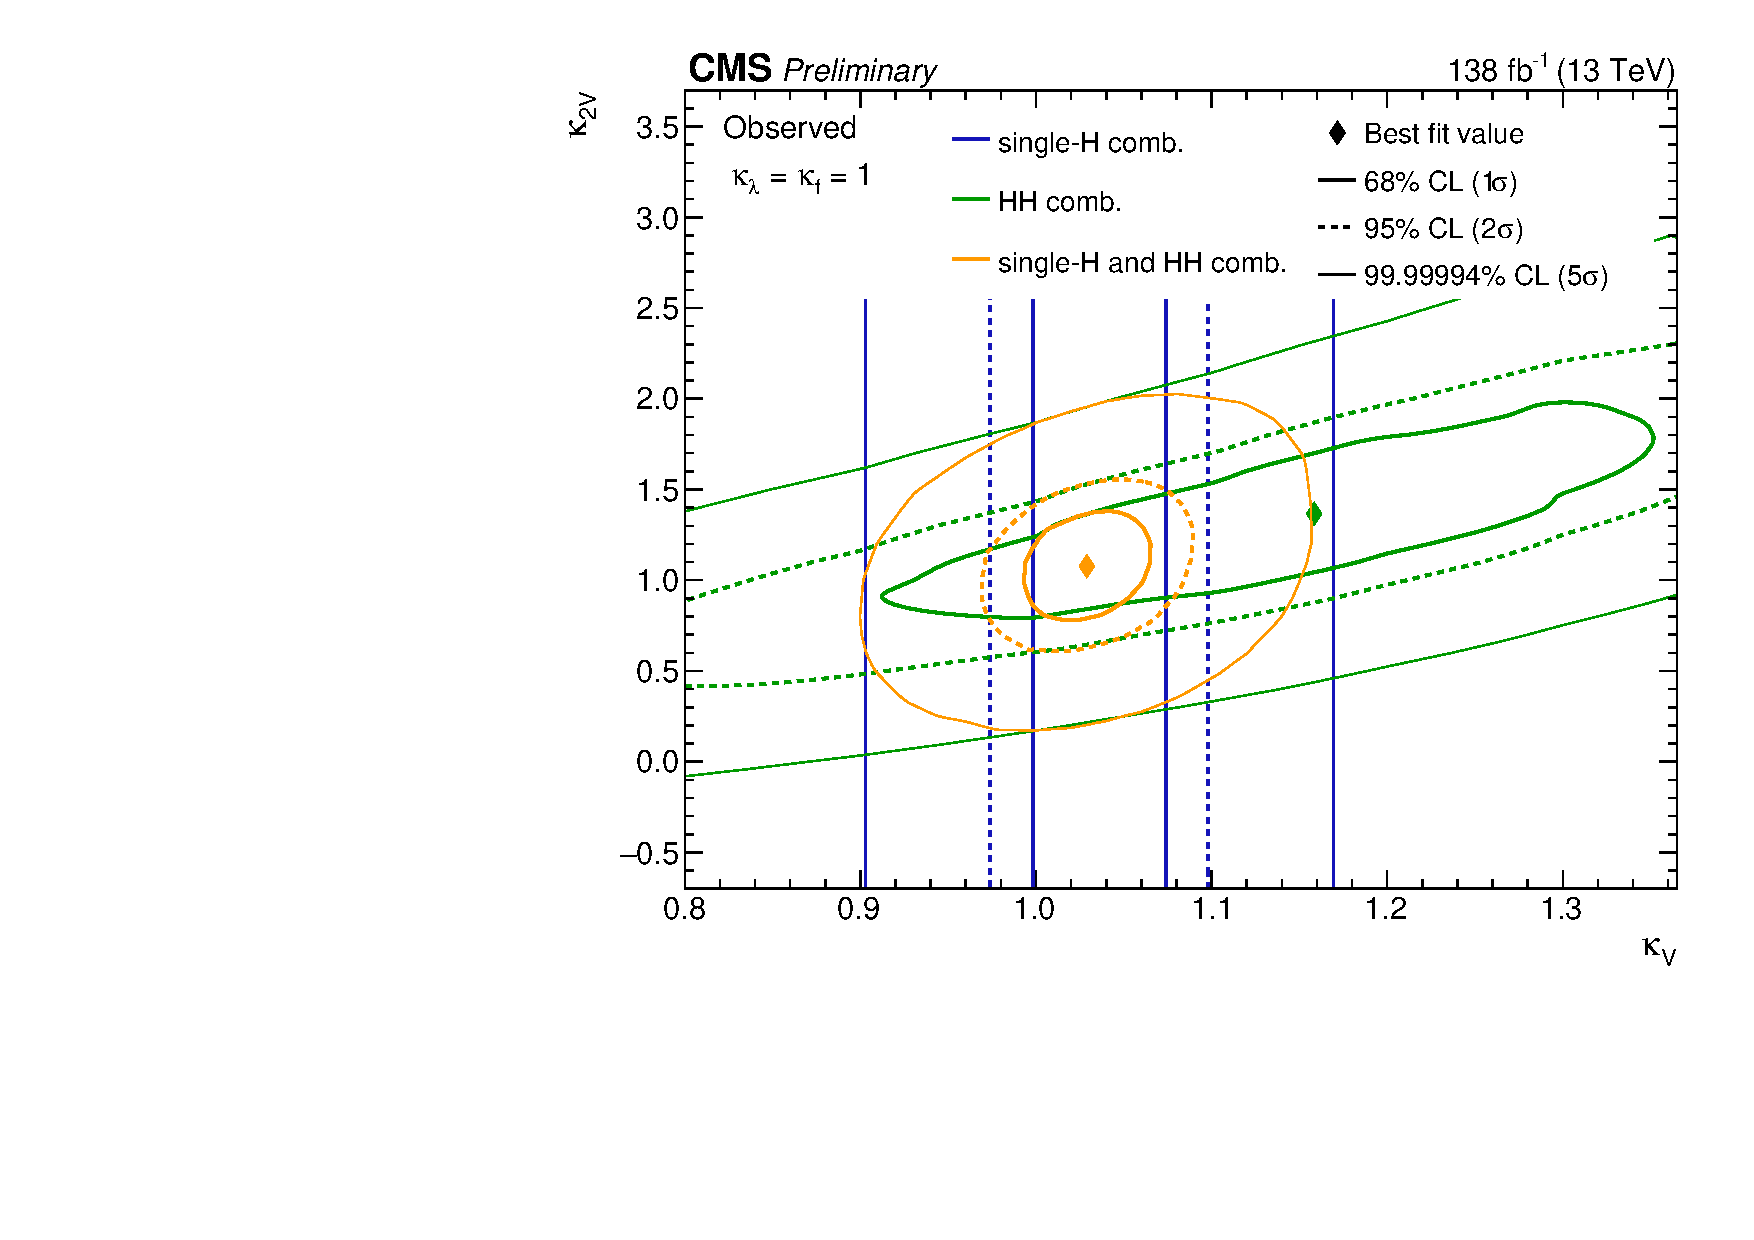
\includegraphics[width=.5\textwidth]{/home/bruno/org/PhD/Thesis/figures/combination_single_double_k2v_kv.pdf}
\caption{\label{fig:combination_2d_scans}Observed two-dimensional likelihood scans of (\(\kl\), \(\kt\)) (left) and (\(\kv\), \(\kvv\)) (right). The strong complementarity between the single and double Higgs processes is well illustrated. The remaining coupling modifiers are set to their \ac{SM} value. Taken from \cite{CMSHplusHHcomb}.}
\end{figure}
\subsection{Going beyond the SM}
\label{sec:org9bac781}
\subsubsection{SM shortcomings}
\label{sec:org0ec8295}
\label{sec:SMShortComings}

CP violation / matter-antimatter asymmetry \cite{cp_violation1,cp_violation2,cp_violation3}
\begin{enumerate}
\item Electro-weak phase transition
\label{sec:org5f9fe36}
\label{sec:ewpt}

As discussed in Section \cref{sec:SM}, the existence of the Higgs field breaks electro-weak symmetry.
However, at extremely high temperatures, it is energetically favourable for the Higgs field to be zero everywhere.
Only around a hundred picoseconds after the Big Bang, as the temperature of the Universe drops beneath a threshold, is the symmetry broken.
It is currently unknown how the symmetry breaking takes place.
While the SM predicts a smooth transition, a plethora of BSM models prefers a first-order phase transition.

\begin{itemize}
\item possibility of the existence of false vacua, where our Universe may lie (``metastable'')
\item discuss consequences, namely vaccum decay, creating vaccum bubbles, possibly (but unlikely) destroying the Universe as we know it
\item electro-weak baryogenesis: the existence of vaccum bubble in the early universe can explain the observed matter-antimatter assymetry
\item the singlet model, although being the simplest extenson possible to the SM, can generate a strong first-order electro-weak phase transition sufficient for electro-weak baryogenesis
\item examine the Higgs field more precisely, since new states can alter the shape of the Higgs potential, as weel as its behaviour as a function of temperature
\item unnaturalness between Planck and electro-weak scales mentioned in Section \cref{sec:SMShortComings}
\item possibly link with sakharov conditions (????)
\end{itemize}

As Eq. \cref{eq:sm_potential} shows,
\end{enumerate}
\subsubsection{Non-resonant BSM HH Production}
\label{sec:org3b486b7}
\label{sec::NonResBSMHH}

Many models of physics beyond the Standard Model with \ac{SM}-compatible single Higgs boson signal strengths can exhibit a di-Higgs phenomenology vastly different from the \ac{SM} expectation.
In this sense, a successful discovery of Higgs boson pair production at the LHC and the subsequent measurement of potential deviations from the \ac{SM} constitute an important avenue in the search for physics beyond the \ac{SM}.

To facilitate such a measurement, it is crucial to establish the Higgs boson pair production cross section in the \ac{SM} to the best theoretical accuracy possible and to provide \ac{BSM} benchmarks that reflect the phenomenology of Higgs boson pairs at the LHC in a consistent and concise fashion.

\begin{figure}
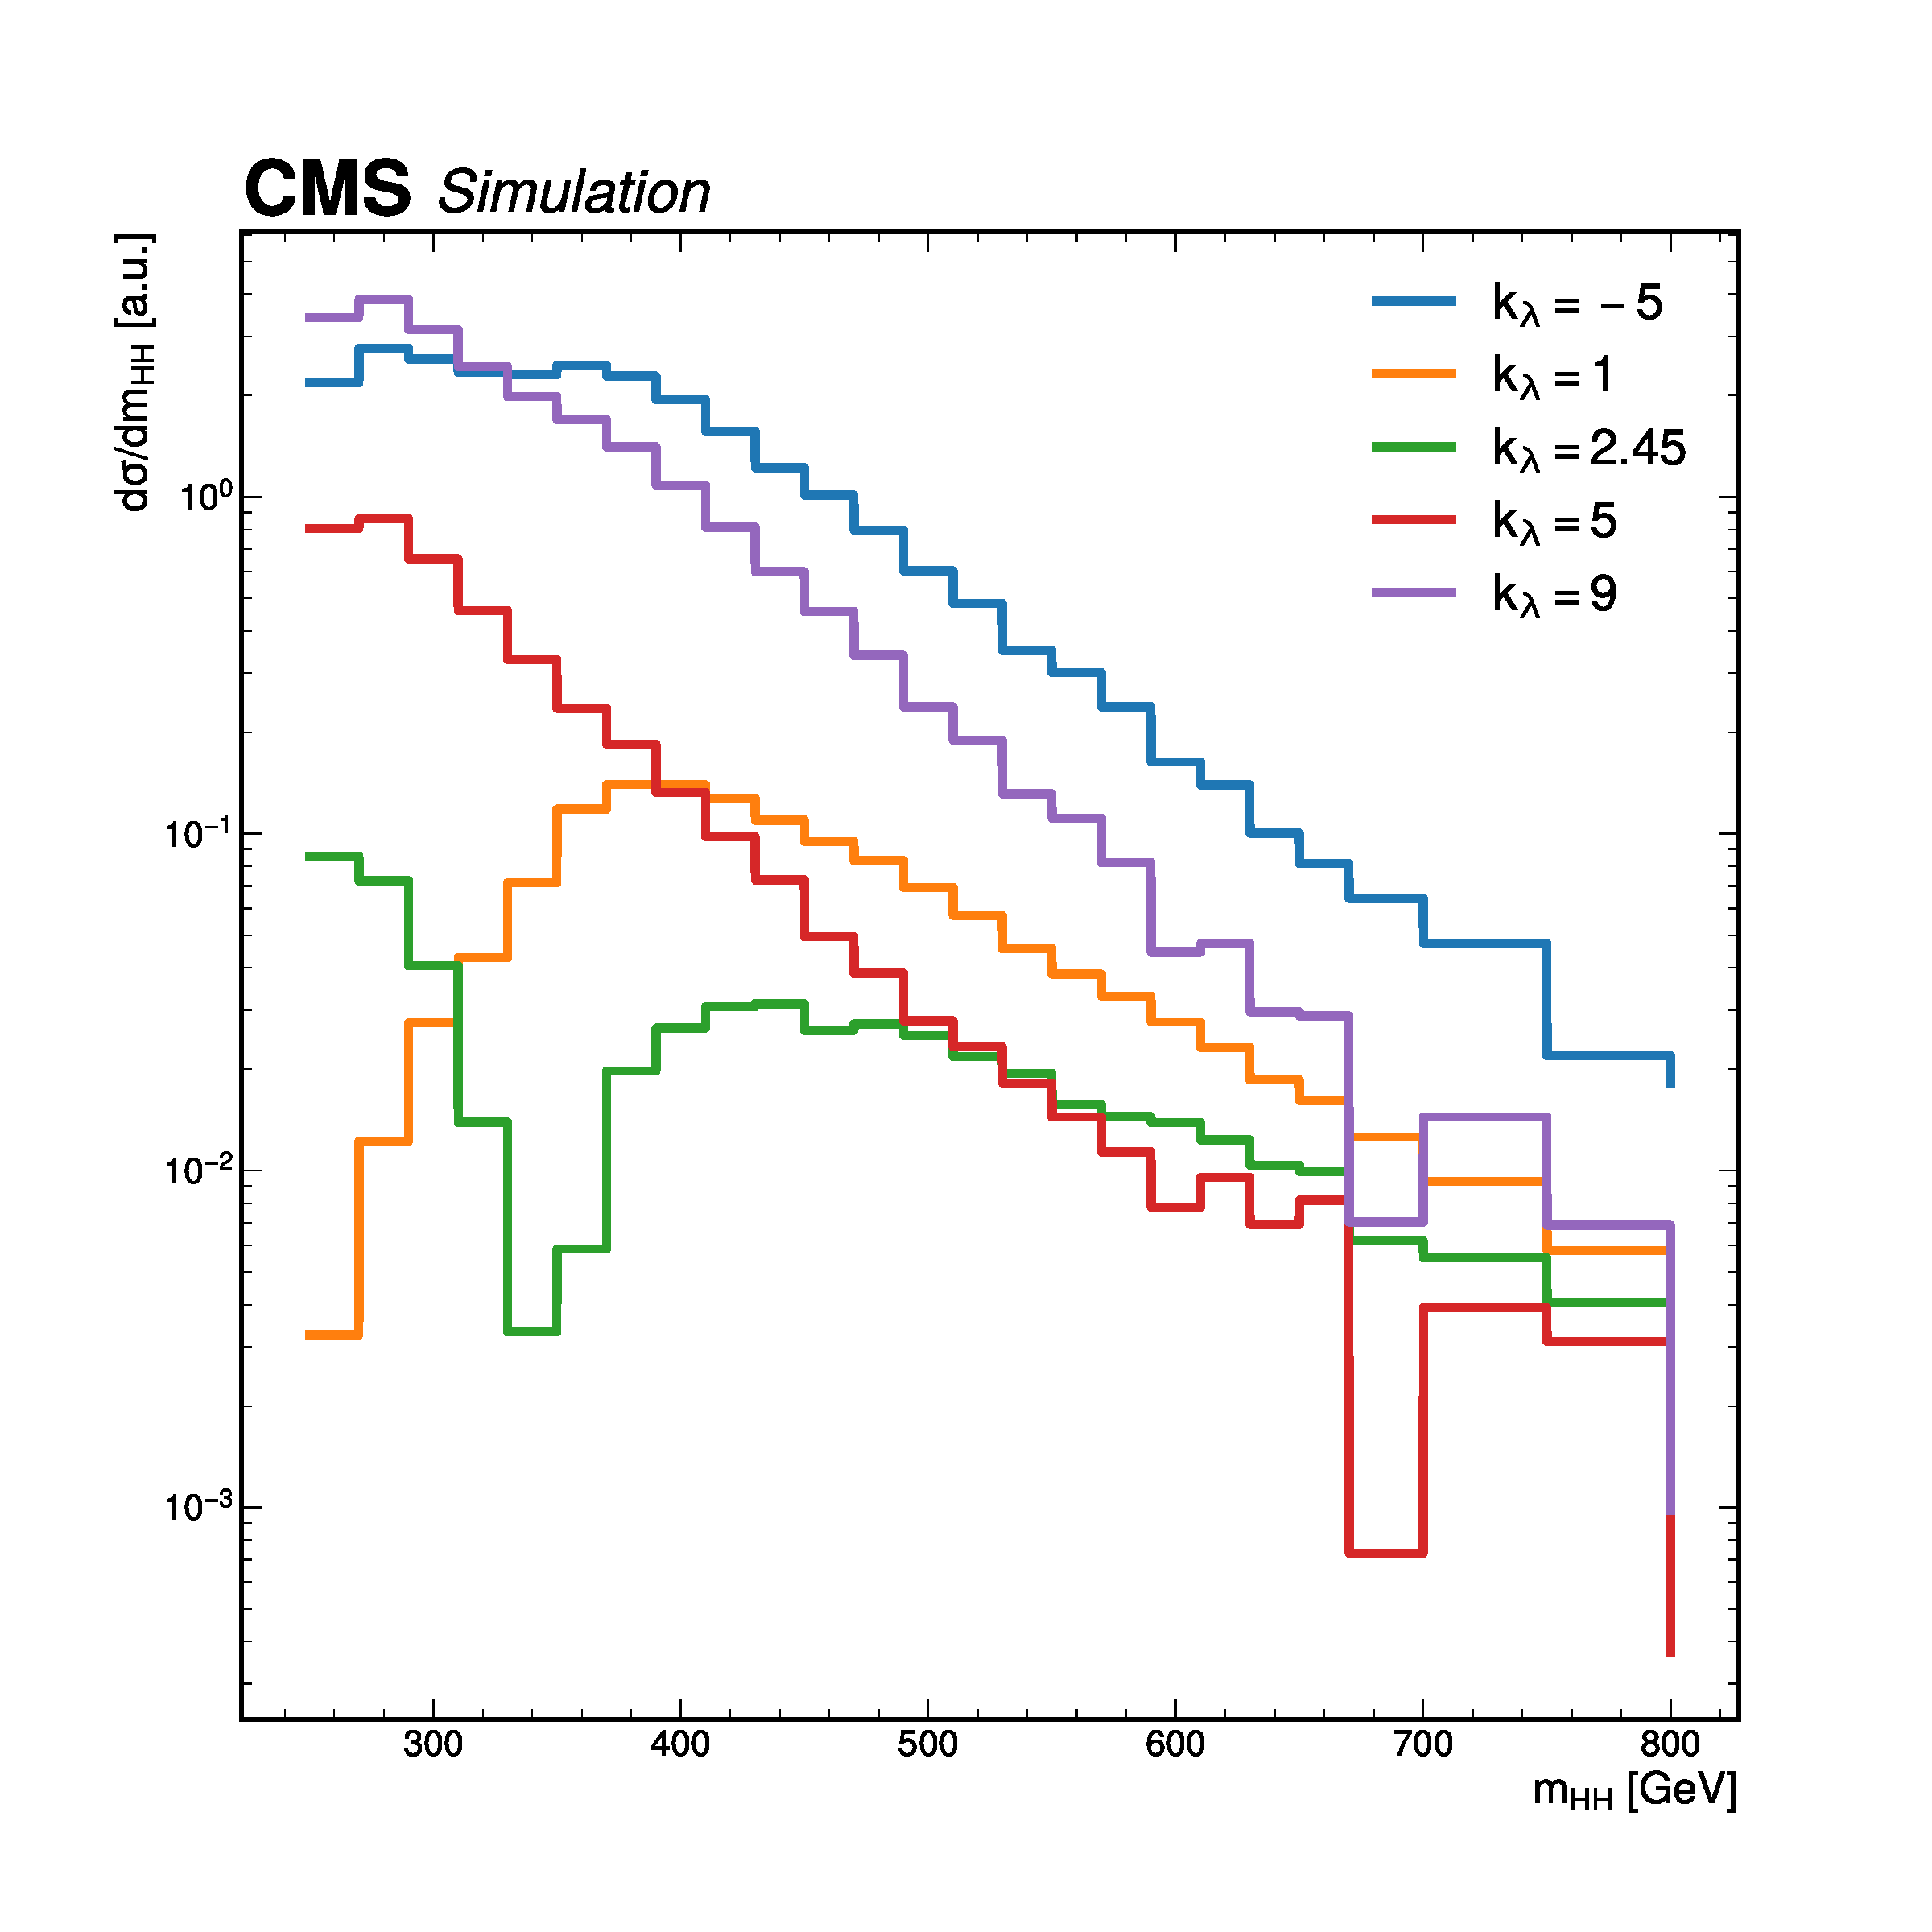
\includegraphics[width=.5\textwidth]{/home/bruno/org/PhD/Thesis/figures/intro/kl.pdf}
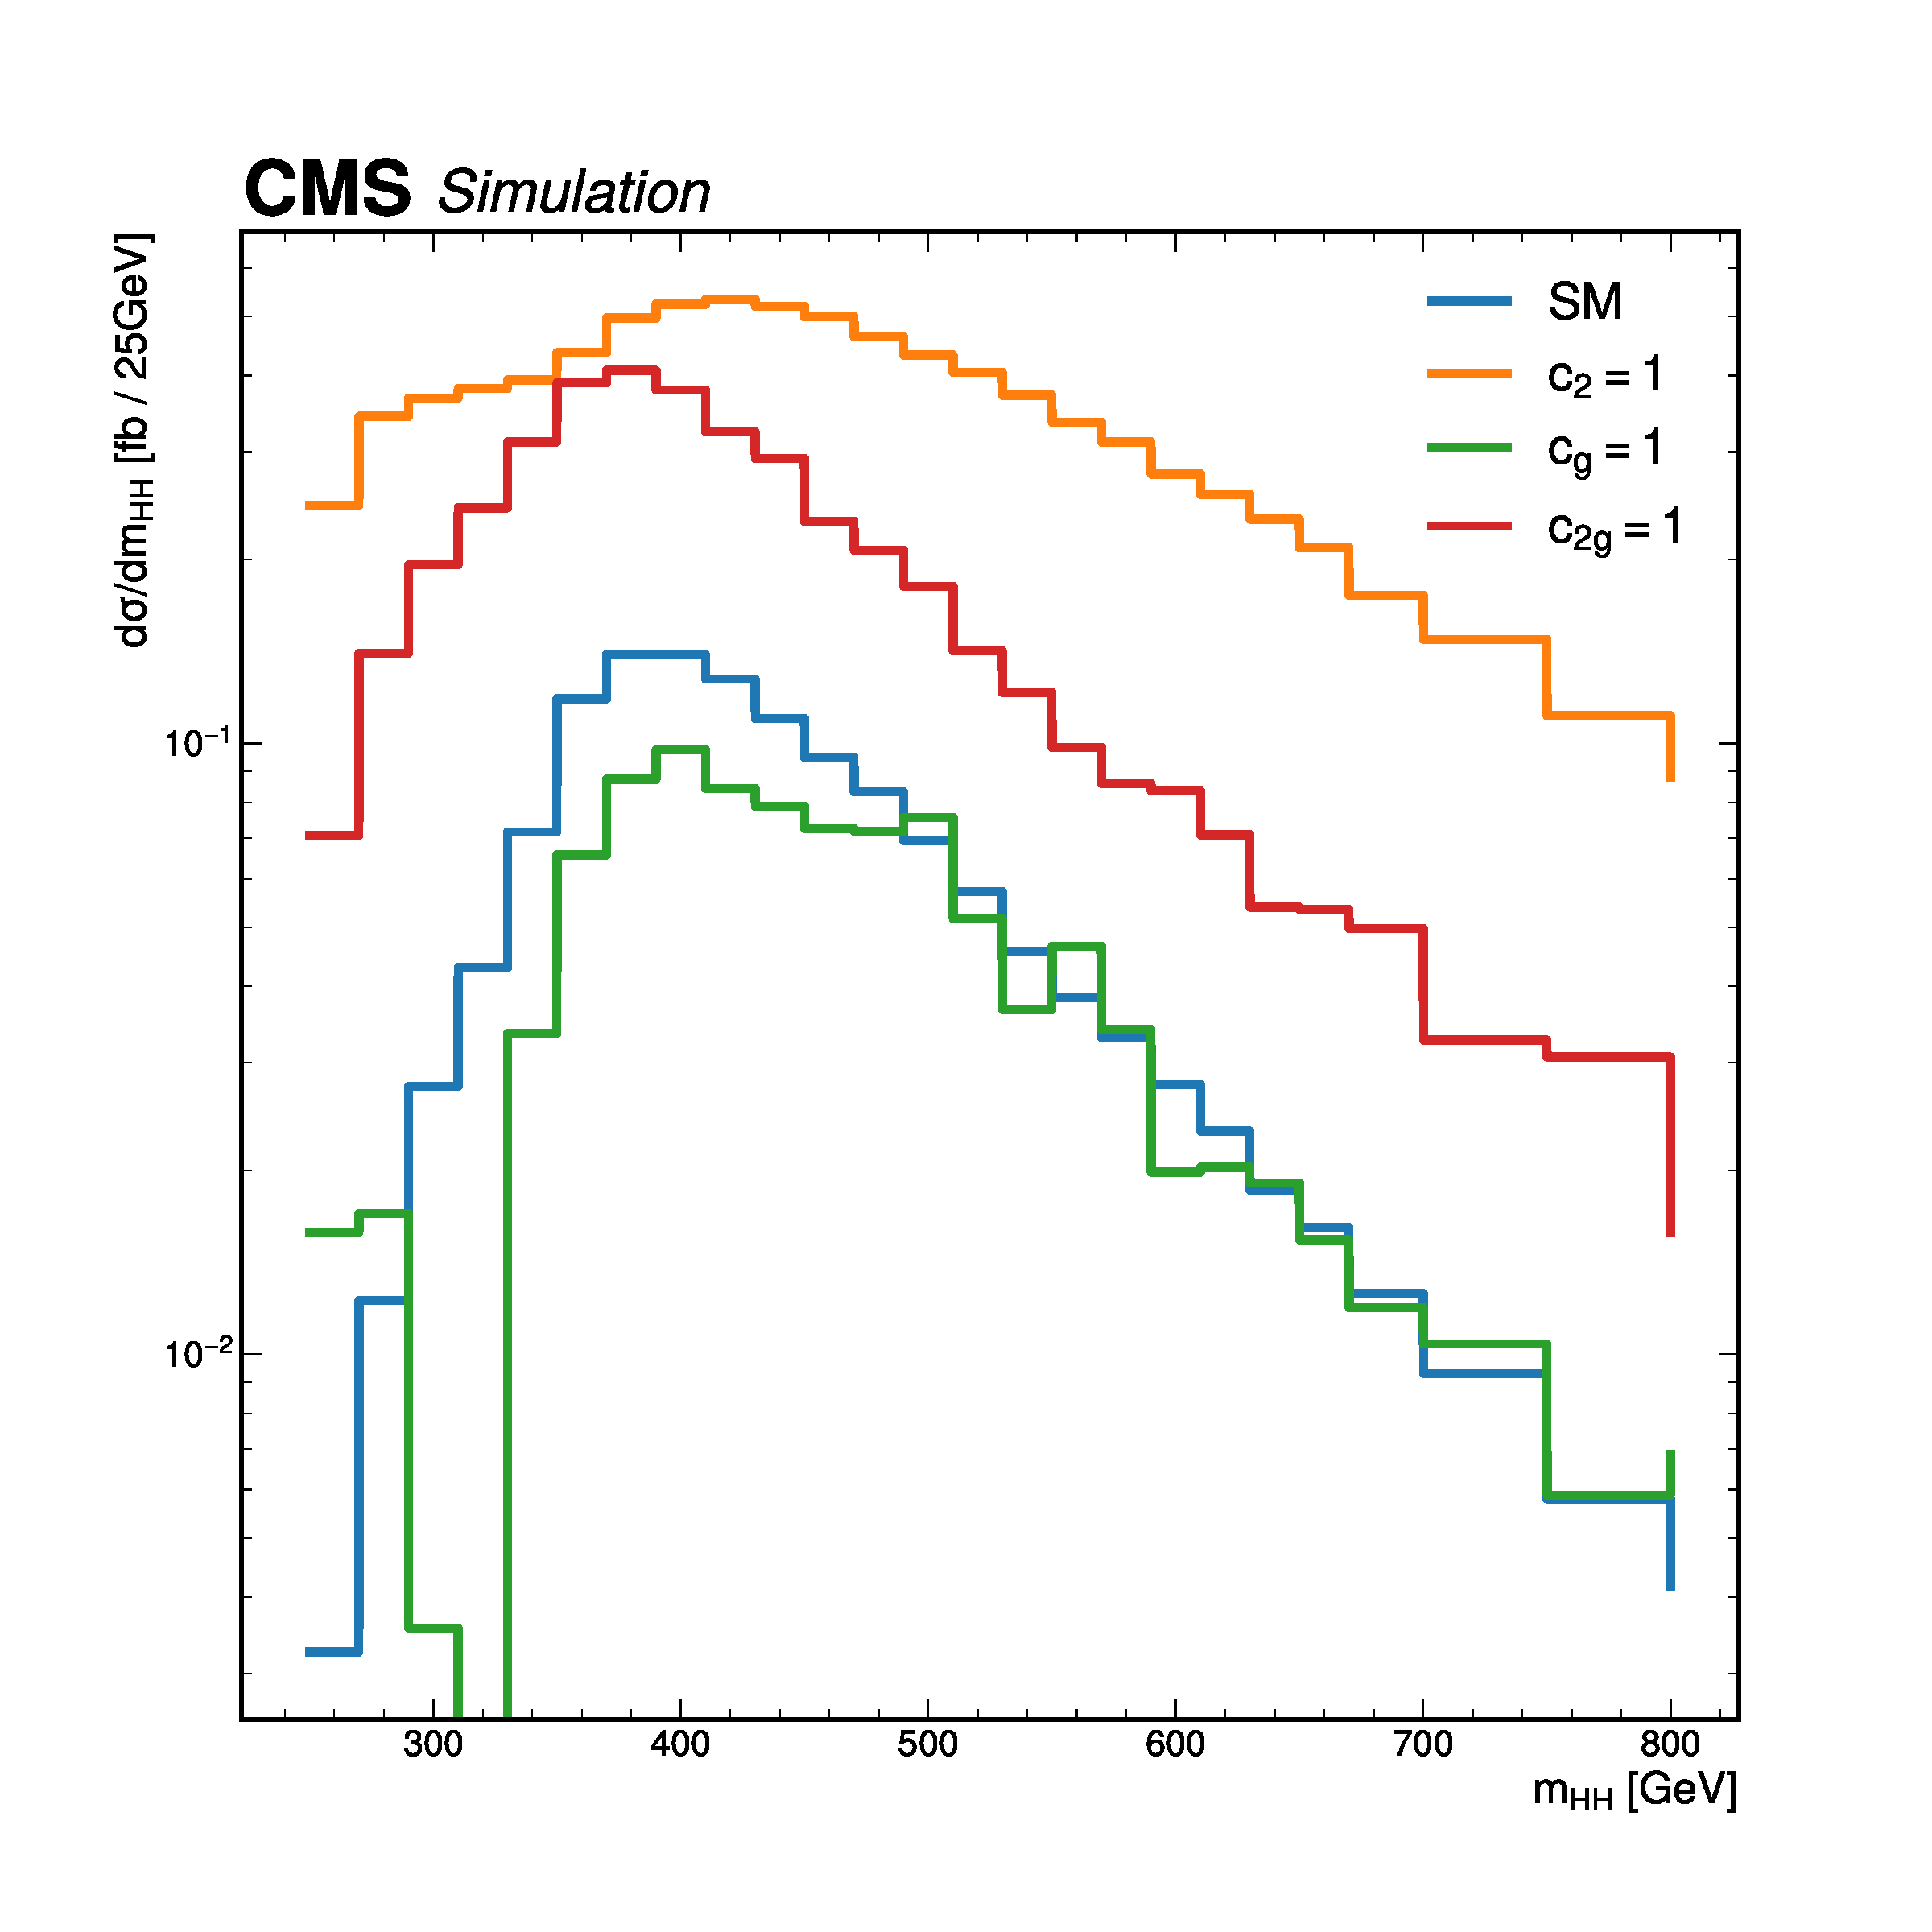
\includegraphics[width=.5\textwidth]{/home/bruno/org/PhD/Thesis/figures/intro/c.pdf}
\caption{\label{fig:kl_c_EFT}HH mass distribution for different \(\kl\) values, highlighting the strong impact of a deviation from the expected SM values. Larger \(|\kl|\) values correspond to scenarios where the HH ``triangle'' diagram dominates.}
\end{figure}

See \cref{fig:kl_c_EFT} now!

Test \ac{BSM} w/ anomalous couplings
\begin{itemize}
\item discuss coupling modifiers
\item deviations may lead to diffs. in HH production and kinematics
\item small SM HH cross-section because of the interference between the triangle nad box diagrams
\end{itemize}
\begin{enumerate}
\item Effective Field Theories
\label{sec:org298426d}
\begin{itemize}
\item Probe effects from resonances with very high mass at lower energy scales
\item \ac{BSM} effects on ggF HH production can be studied
\begin{itemize}
\item through EFT model with three new couplings
\end{itemize}

\item Explore sensitivity to \ac{BSM} \ac{EFT} couplings with \ac{EFT} benchmark points
\begin{itemize}
\item based on test statistic measuring kinematics’ similarities
\item allow extrapolation between different points
\end{itemize}
\end{itemize}
\end{enumerate}
\subsubsection{Resonant BSM HH Production}
\label{sec:orgc8c0df7}
\label{sec::ResBSMHH}
\begin{enumerate}
\item Motivaton for the bb\(\tau \tau\) analysis
\label{sec:org7e6d3fa}
\end{enumerate}
\section{The CMS Detector at the LHC}
\label{sec:orgca88d19}
\subsection{The Large Hadron Collider}
\label{sec:orgb6b9a07}
\label{sec:lhc_intro}

The Large Hadron Collider (LHC) is one of the largest scientific instruments ever built.
Since opening up a new energy frontier for exploration in 2010, it has gathered a global user community of about 9000 scientists working in fundamental particle physics and the physics of hadronic matter at extreme temperature and density \cite{hllhc}.
\subsubsection{Design}
\label{sec:org70060d1}
\label{sec:lhc_design}

It is common practice to express charged and neutral particle contributions to radiation in terms of dose and \SI{1}{\MeV} neutron equivalent fluence, respectively.
The term (absorbed) dose refers to the mean energy imparted by ionizing radiation to matter in a volume divided by the mass contained in the respective volume \cite{icru_report}.
Any particle fluence can be reduced to an equivalent 1 MeV neutron fluence producing the same bulk damage in a specific semiconductor. The scaling is based on the hypothesis that generation of bulk damage is due to non-ionizing energy transfers to the lattice.

In the \ac{LHC}, the total Dose and Fluence, cumulated over 10 years of operation, are expected to be about 100
kGy and >1015 particles/cm2 respectively (in the LHC experiments) \cite{fibers_high_dose}

\begin{equation}
\label{eq:lumi}
\frac{\partial N}{\partial t} = L\sigma
\end{equation}

\begin{equation}
\label{eq:inst_lumi}
\mathcal{L} = F \cdot \frac{N_{\text{b}}^2 n_{\text{b}} f_{\text{rev}} \gamma}{4\pi \epsilon_n \beta^*}
\end{equation}

\begin{equation}
\label{eq:lumi_form_fact}
F = \left( 1 + \frac{\theta_{\text{c}}\sigma_z}{2\sigma_{xy}} \right)^{\frac{-1}{2}}
\end{equation}

\begin{equation}
\label{pileup}
<\mu> = \frac{L\sigma_{pp}^{\rm inelastic}}{n_bf_{\rm rev}}
\end{equation}

\begin{table}[!h]
\centering
\begin{tabular}{c|c|c}
Parameter & Description & Value\\
\hline
\(\sqrt{s}\) & centre-of-mass energy & \SI{14}{\TeV}\\
\(N_{\text{b}}\) & particles per bunch & \num{1.15e11}\\
\(n_{\text{b}}\) & number of bunches per beam & \num{2808}\\
\(f_{\text{rev}}\) & revolution frequency & \SI{11.2}{\kilo\hertz}\\
\(\epsilon_n\) & transverse beam emittance & \SI{3.75}{\micro\meter}\\
\(\beta^*\) & beta function (focal length) & \SI{0.55}{\meter}\\
\(\Delta t_{\text{b}}\) & bunches spacing & \SI{25}{\nano\second}\\
\(\theta_{\text{c}}\) & collision angle & \SI{285}{\micro\radian}\\
\(\sigma_z\) & bunches transverse r.m.s at IP & \SI{7.55}{\cm}\\
\(\sigma_{xy}\) & bunches longitudinal r.m.s at IP & \SI{16.7}{\micro\meter}\\
\end{tabular}
\caption{\label{tab:LHCparameters}Nominal design parameters of the LHC machine in proton-proton collisions configuration.}

\end{table}

Goal for Run 3 is to approx. double the luminosity for ATLAS and CMS

\begin{figure}
\includegraphics[width=1.\textwidth]{/home/bruno/org/PhD/Thesis/figures/detector/CERNaccelerators.pdf}
\caption{\label{fig:econt_algorithms}Representation of the CERN accelerator complex. The LHC is the last ring (dark blue line) in a complex chain of particle accelerators. The smaller machines are used in sequence to accelerate the proton beams that collide in the centre of the four main detectors. Taken from \cite{lhc_complex}.}
\end{figure}
\subsubsection{Operations}
\label{sec:org6479af6}
\label{sec:lhc_operatoins}

.
\begin{figure}
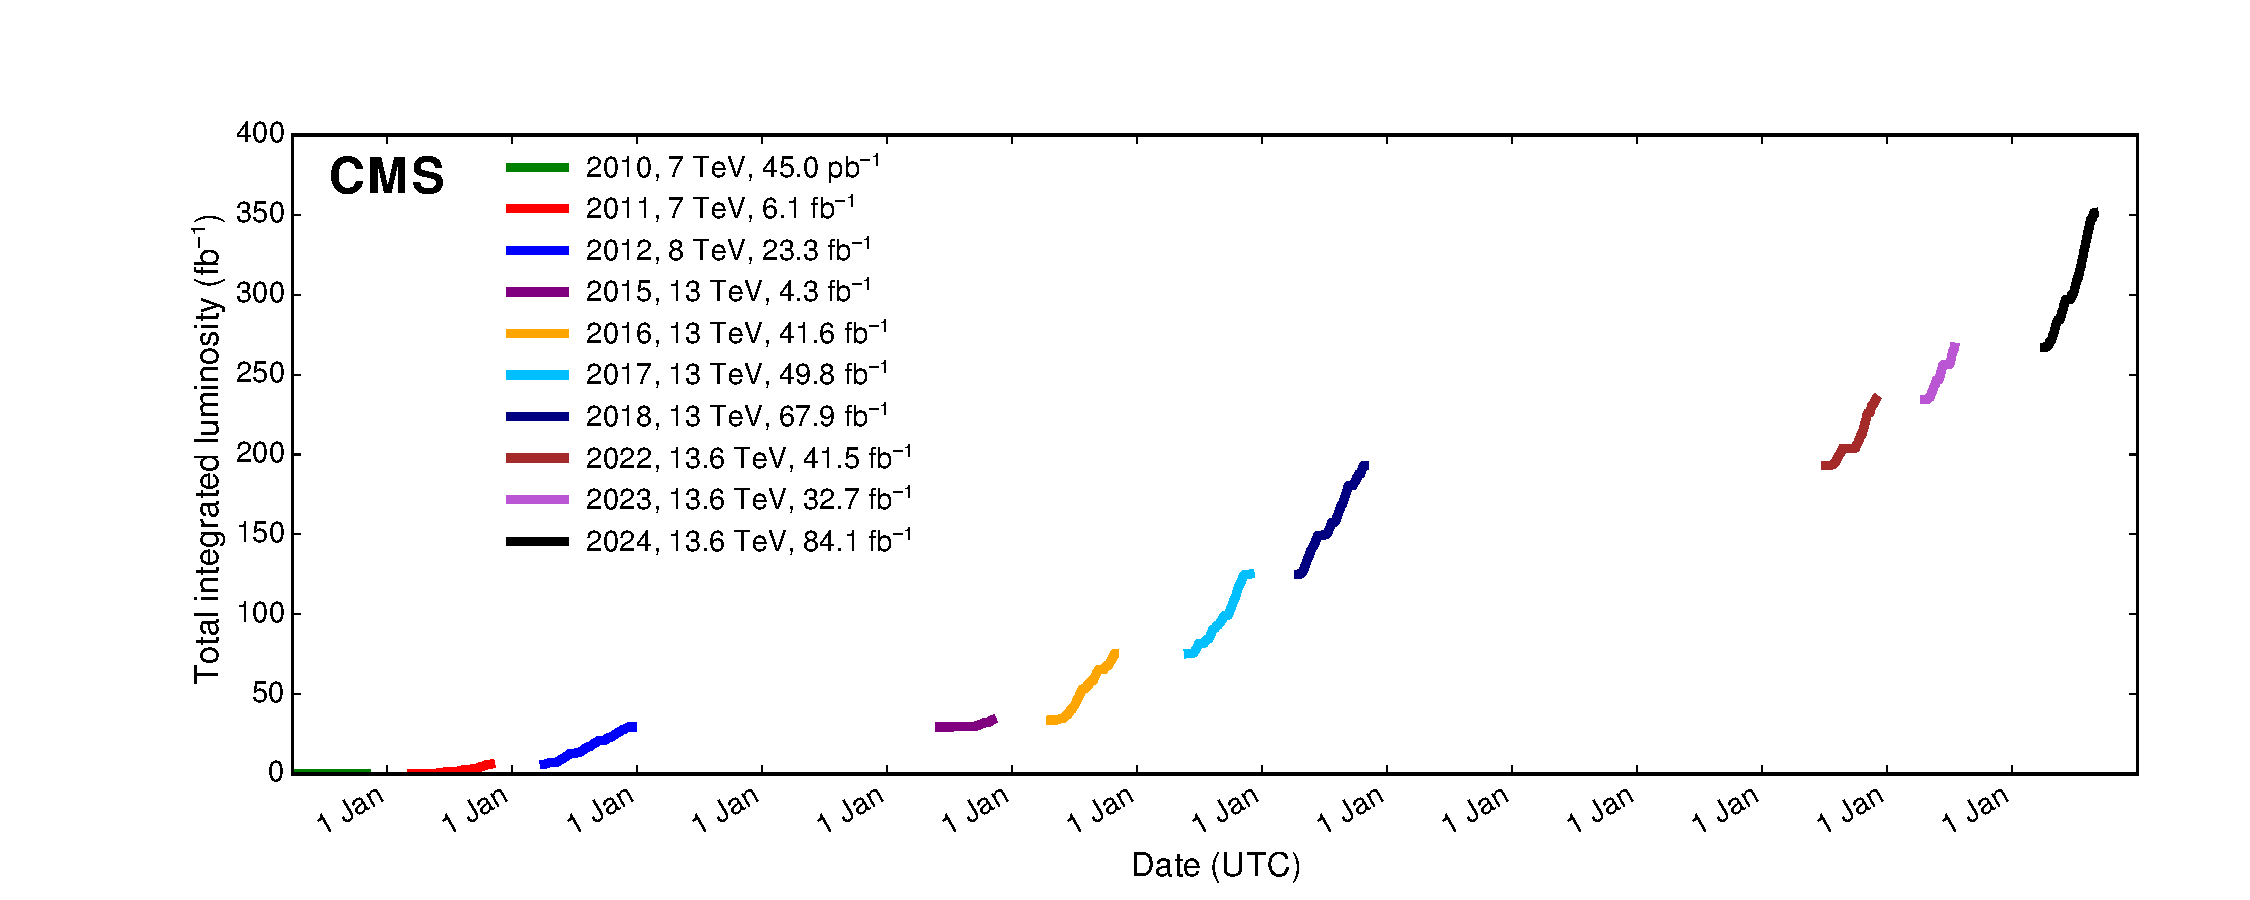
\includegraphics[width=1.\textwidth]{/home/bruno/org/PhD/Thesis/figures/hgcal/lhc/int_lumi_cumulative_pp.pdf}
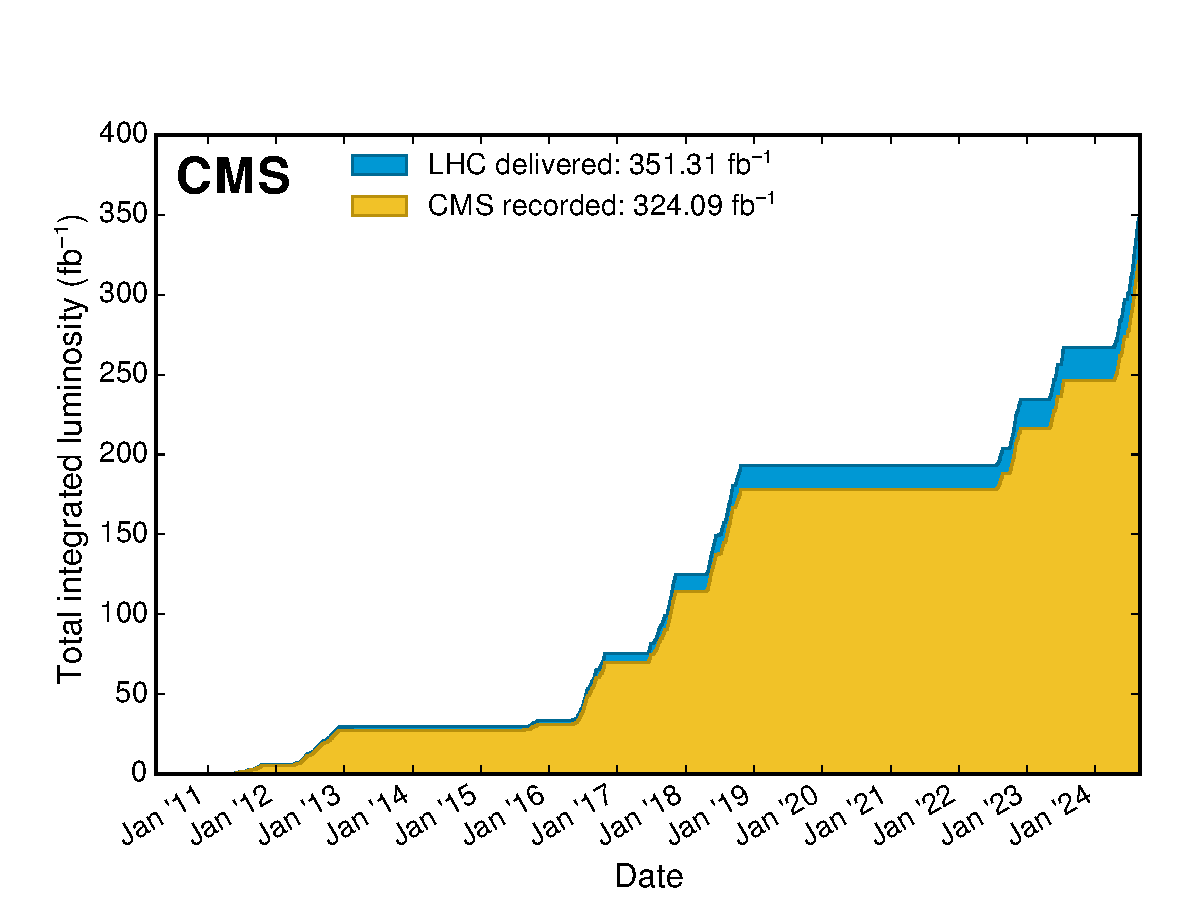
\includegraphics[width=.525\textwidth]{/home/bruno/org/PhD/Thesis/figures/hgcal/lhc/int_lumi_allcumulative_pp.pdf}
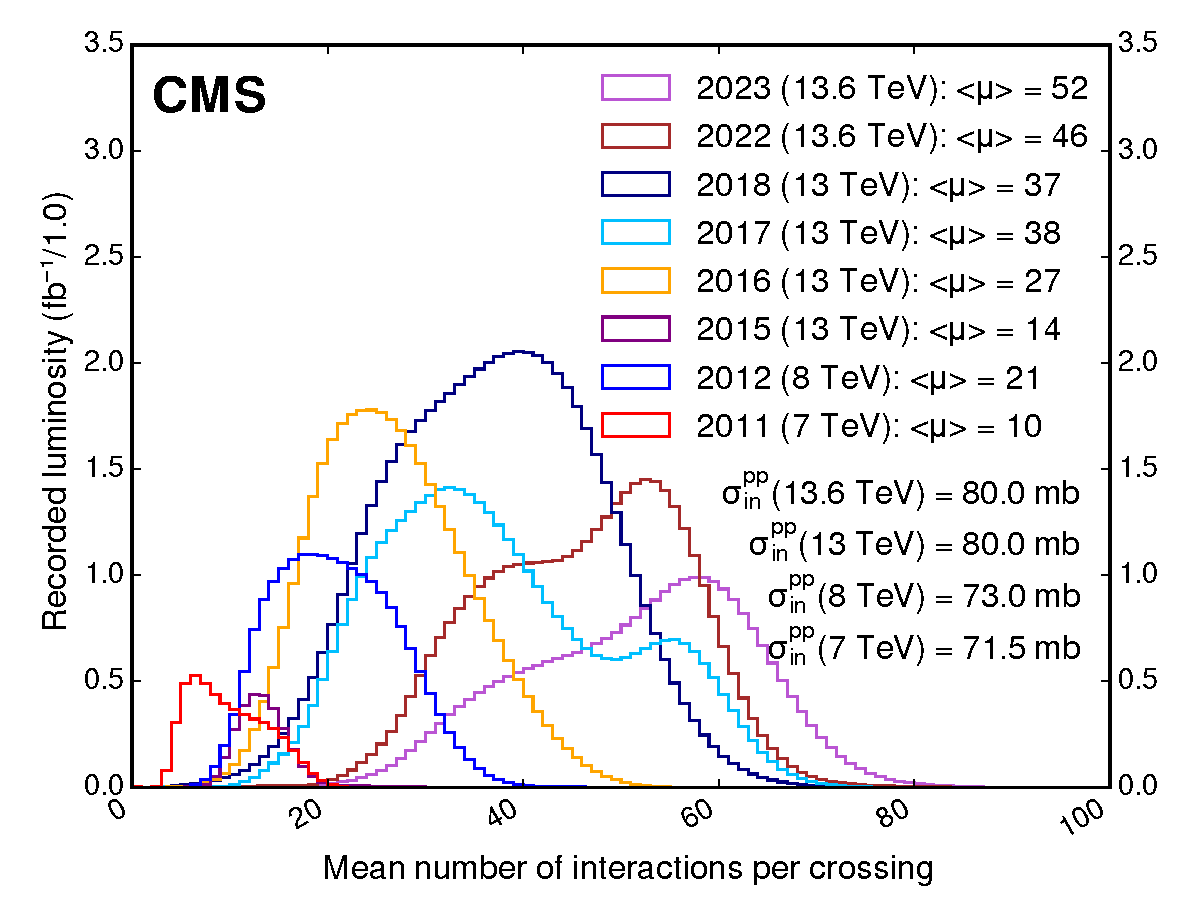
\includegraphics[width=.475\textwidth]{/home/bruno/org/PhD/Thesis/figures/hgcal/lhc/pileup_allYears.pdf}
\end{figure}
\subsubsection{Experiments}
\label{sec:orgbed4280}
\label{sec:lhc_experiments}

In the following we provide a summary of some of the most emblematic physics experiments at the \ac{LHC}, before describing the \ac{CMS} detector in \cref{sec:cms_detector}.

\paragraph{NA62}
The NA62 experiment operates a 27X0 (1.25 m) deep LKr calorimeter at CERN’s SPS, which earlier served the predecessor experiment NA48 [4].
Its em energy resolution was measured with electrons at high energies (10–80 GeV).
\cite{wigmans2}

\paragraph{ATLAS}
\begin{itemize}
\item General-purpose detector. \cite{atlas_collab}
\item The ATLAS electromagnetic calorimeter
\end{itemize}
{[}103] uses a lead/liquid argon sampling technique, with an ‘accordion’ geometry,
and is located outside of the inner solenoid. The liquid argon technique was chosen
for its immunity to radiation, its intrinsic stability and linearity of response, and its
relative ease of longitudinal and transverse segmentation. Its more modest intrinsic
resolution is a limiting factor at medium and low energies. The calorimeter features three segments in depth, the first one having an extremely fine segmentation in pseudorapidity (0.003) to allow separation between prompt photons and photons from π0 decays up to pT \textasciitilde{} 70 GeV/c, the interesting range for the Higgs boson search in the γγ decay mode.
The calorimeter is preceded by a presampler, located in the same cryostat, to
correct for the loss of energy of electrons and converted photons in the inner detector
material, in the solenoid and cryostat front walls (see Table 6.5). The barrel part,
consisting of two cylinders, and the two end-cap wheels provide uniform azimuthal
coverage despite being built of 16 (8) modules per cylinder (wheel) (Fig. 6.46). \cite{calorimetry_fabjan}

\paragraph{LHCb}

Instead of surrounding the entire collision point with an enclosed detector as \ac{ATLAS} and \ac{CMS} do, the \ac{LHCb} experiment \cite{lhcb_collab}, located at \ac{IP} 8, employs a single-arm forward spectrometer.
The experiment includes large aperture subdetectors (\SIrange{10}{300}{\milli\radian}) placed perpendicularly to the beam axis.
Given that \ac{LHCb}'s main purpose is the study of \$b\$-flavoured baryons as probes for \ac{NP}, this distinctive design can be readily explained: the decay particles of \(b\) hadrons tend to travel close to the line of the beam pipe.
The design thus exploits to exploit the large \(bb\) production cross section at the \ac{LHC}.
Phenomena studied by \ac{LHCb} include rare B-meson decays, the possible existence of \ac{CP} violating asymmetries in \(b\) and \(c\) hadron decays, the precise measurement of the three interior angles of the \ac{CKM} matrix, \(B_{s}\) mixing, or tests for lepton flavour universality, among many others \cite{lhcb_hllhc_tdr}.

Given the asymmetric geometry of LHCb, to maximally exploit the volume of the underground cavern, the LHC optics is modified  with a displacement of the collision point by \SI{11.25}{\m} from the centre.
Starting from the collision point, and moving outwards through \SI{21}{\m} and \SI{5.6}{\tonne} of subdetectors, \ac{LHCb} presents an array of semi-circular silicon-based detectors composing the \ac{VELO}, followed by the first \ac{RICH} detector, focused on low-momentum tracks.
We note that particle identification is essential to distinguish pion, kaon and proton tracks, notably in flavour physics \cite{lhcb_hllhc_tdr}.
Several layers of the tracker systems follow, separated by a warm dipole magnet \cite{lhcb_collab_tracker_tdr}, and a second \ac{RICH} detector lies just behind the tracker, to measure high-momentum tracks.
We then find a Shashlik electromagnetic calorimeter and a hadronic calorimeter composed of iron and scintillator tiles.
The muon system finalizes the design, enabling impactful measurements such as the study of \(B_{s}^{0}\rightarrow\mu\mu\) decays.

\ac{LHCb} is also the sole \ac{LHC} experiment capable to run both in collider and fixed-target mode \cite{lhcb_fixed_target}.
The \ac{SMOG} provides a mean to inject noble gases (\ch{He}, \ch{Ar}, \ch{Ne}) into \ac{VELO}.
Despite smaller \bb{} cross-sections and worse signal-to-background ratio, fixed-target experiments bring average \(b\) flight lengths of a few\textasciitilde{}\si{\cm}, compared to a few\textasciitilde{}\si{\mm} in the collider mode, due to larger Lorentz boosts.
The larger momenta of the final state particles in the lab also implies simpler triggering and tagging.
Some result bforuhg forward by \ac{SMOG} include fixed-target \jpsi{} and \(D^{0}\) production, and direct measurements of antiproton production \cite{antimatter_prod_fixed_target_lhcb}, which is relevant for \ac{DM} searches.


\cite{bb_pairs1,bbpairs2}
\subsection{The CMS Detector}
\label{sec:org13a188d}
\label{sec:cms_detector}

Detector in Tables \cref{tab_sad} and \cref{tab_sad2}

Use the lead tungstate (\ch{PbWO4}) acronym.

\begin{figure}
\begin{center}
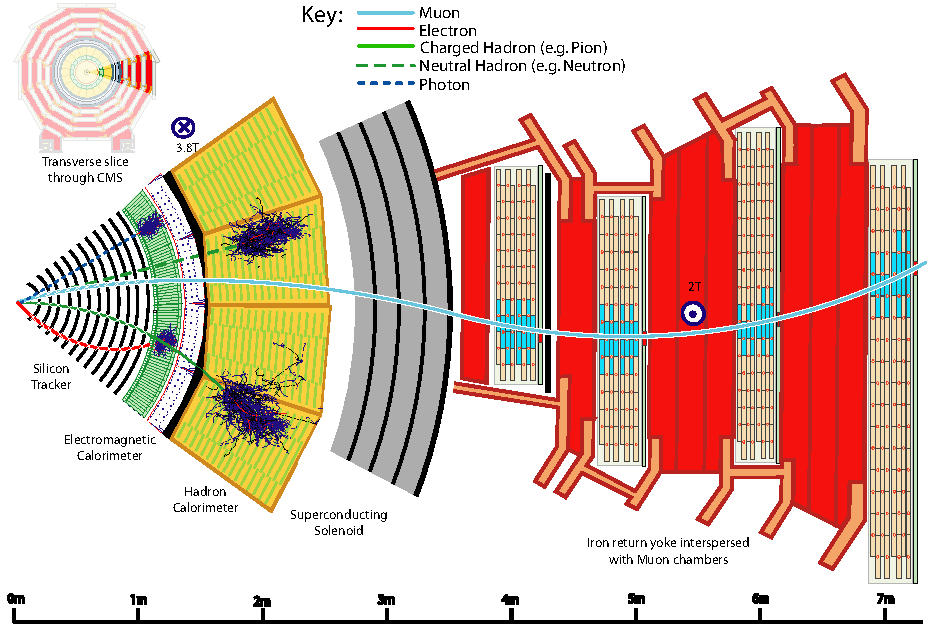
\includegraphics[width=.9\linewidth]{/home/bruno/org/PhD/Thesis/figures/hgcal/CMSslice.pdf}
\end{center}
\caption{\label{fig:cms_slice}Transverse beam interaction slice region of the to the CMS muondetector, detector. The showing muon and the the different charged pion sub-detectors areand how positively different charged, particles and the interact. electron is Figure negatively taken charged. Taken from \cite{particle_flow_cms}.}
\end{figure}


\begin{figure}
\begin{center}
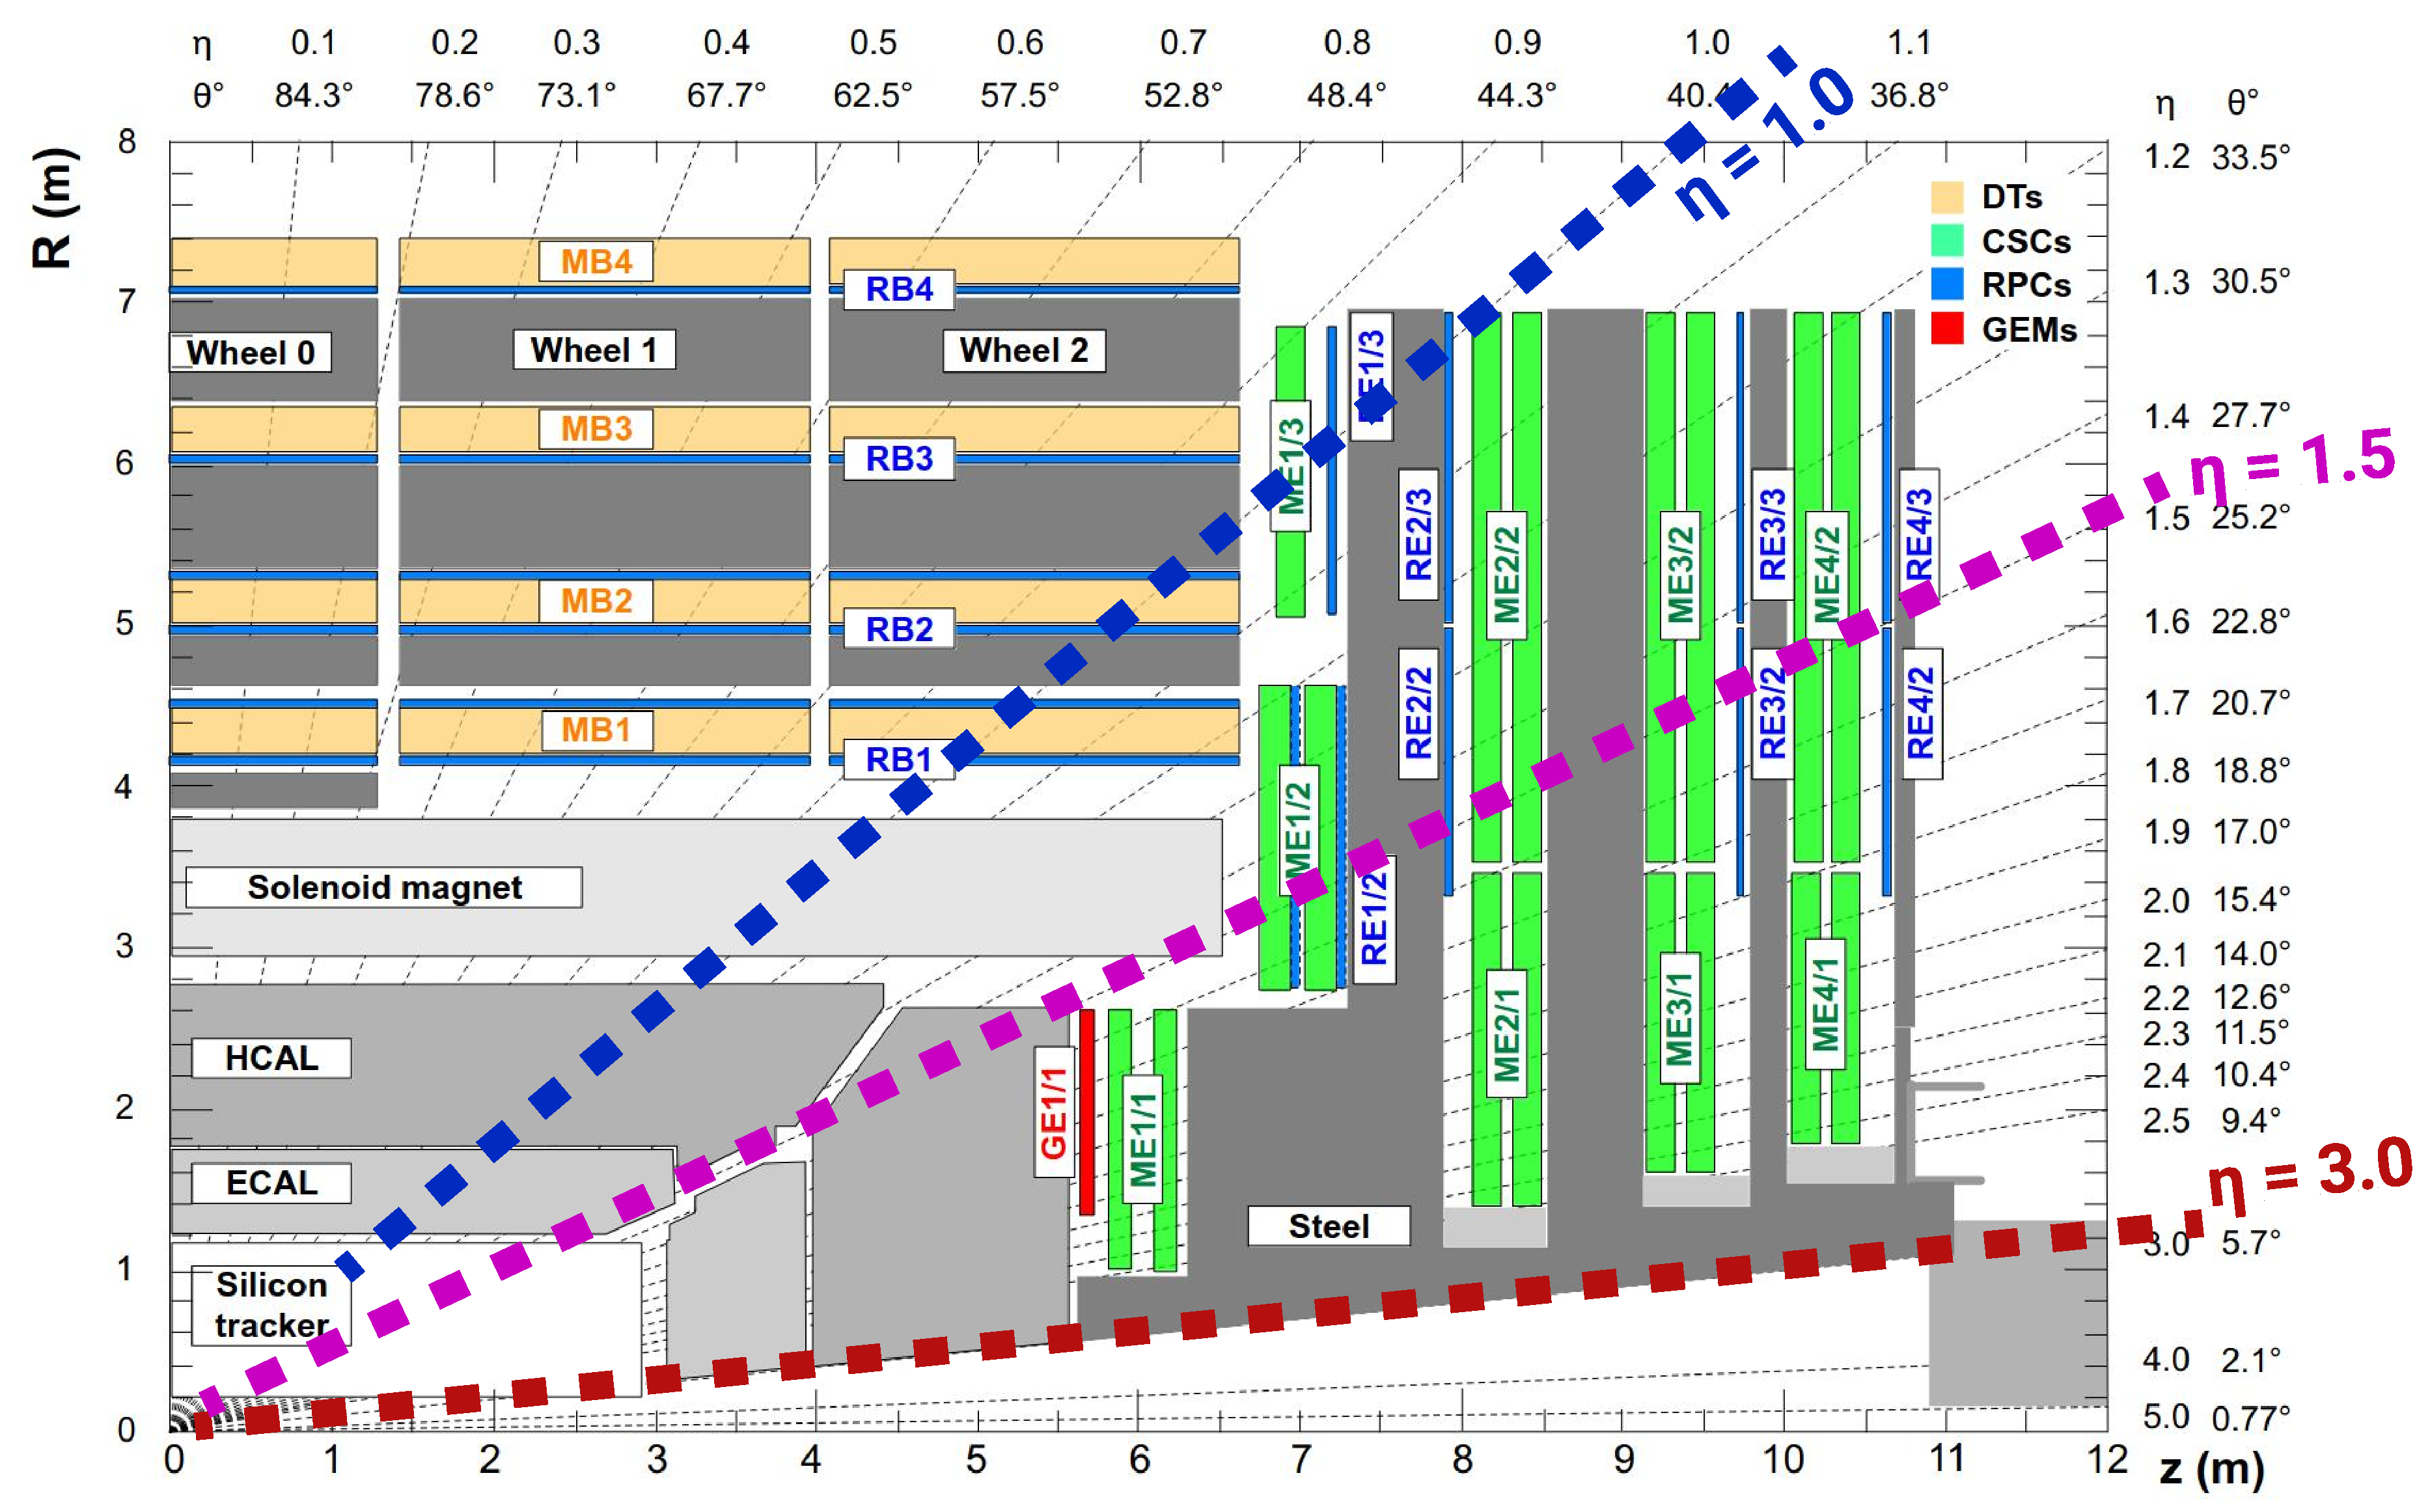
\includegraphics[width=.9\linewidth]{/home/bruno/org/PhD/Thesis/figures/intro/MuonSystem.pdf}
\end{center}
\caption{\label{fig:cms_slice}Schematic longitudinal view of a quadrant of the R-z cross-section of the \ac{CMS} detector. All four subdetector are shown: \acp{DT} (yellow), \acp{CSC} (green), \acp{RPC} and \acp{GEM}. Pseudorapidity values are given with dashed lines, and some values are highlighted. Adapted from \cite{gem_tdr}.}
\end{figure}

\begin{table}[htbp]
\centering
\begin{tabular}{ll}
dsd & \\
\hline
\end{tabular}
\caption{\label{tab_sad}sad}

\end{table}

\begin{table}[htbp]
\centering
\begin{tabular}{ll}
dsd & \\
\hline
\end{tabular}
\caption{\label{tab_sad2}sad}

\end{table}
\subsubsection{Coordinate system}
\label{sec:org056019d}
The CMS experiment adopts a right-handed coordinate system, with the origin placed at the nominal collision point.
The x-axis points toward the centre of the LHC ring, the y-axis points vertically upward, and the z-axis thus points towards the Jura mountains.
The structure of the detector makes it natural to use a polar coordinate system.
The azimuthal angle \(\phi\) is measured in the \(x - y\) plane from the x-axis, the radial coordinate is given by \(r\), and the polar angle \(\theta\) is measured from the z-axis in the \(y - z\) plane.
A schematic representation of the CMS coordinate system is shown in Fig. 2.5.
The relation between the Cartesian and the CMS coordinates is given by:

\begin{equation}
\label{eq:xyzcoords}
\begin{cases}
x = r \sin \theta \cos \phi \\
y = r \sin \theta \sin \phi \\
z = r \cos \theta
\end{cases}
\end{equation}

While this coordinate system is well suited for expressing the orientation of the detector and macroscopic observables, it is not ideal for describing proton-proton collisions.
A proton-proton collision is actually a parton-parton collision.
Protons, not being fundamental particles, are made of different constituents, named partons.
Consider a scenario where two protons collide head-on.
The four-momentum of the two partons can be written as:

\begin{equation}
\label{eq:momenta}
\begin{cases}
p^{\mu}_1 = (x_1E, 0, 0, x_1p) \\
p^{\mu}_2 = (x_2E, 0, 0, -x_2p) \\
\end{cases}
\end{equation}

In these four-vectors, \(E\) and \(p\) denote the energy and momentum of the proton, respectively.
The \(x\) and \(y\) components are null as protons are primarily accelerated longitudinally at high energies, leading to negligible transverse momentum for the partons inside them.
Consequently, the \(x_1\) and \(x_2\) variables can be interpreted as the fractions of energy that the partons carry away from the original protons.
After the collision, the resulting momentum is given by:

\begin{equation}
\label{eq:pmomenta}
(p_1 + p_2)^{\mu} = ((x_1 + x_2)E, 0, 0, (x_1 - x_2)p)
\end{equation}

The CMS frame is not the centre-of-mass frame of the collision.
The relativistic \(\beta\) factor, in the high-energy limit where \(E \approx p\), results to be:

\begin{equation}
\label{eq:beta}
\beta = \frac{x_1 - x_2}{x_1 + x_2}
\end{equation}

The \(x_1\) and \(x_2\) quantities are unknown and change from event to event, consequently also the related Lorentz-boost is unknown.
It is thus beneficial to use variables that are Lorentz-invariant for boosts along the longitudinal direction.
The par excellence observables are the transverse momentum \(p_T\) and transverse mass \(m_T\):

\begin{equation}
\label{eq:transverse_momenta}
\begin{cases}
p^2_T = p^2_x + p^2_y \\
m^2_T = m^2 + p^2_x + p^2_y = E^2 - p^2_z \\
\end{cases}
\end{equation}


From these variables, the transverse energy is defined as:
\begin{equation}
\label{eq:transverse energy}
E^2_T = m^2 + p^2_T
\end{equation}

which is equal to the transverse momentum for massless particles.
Another variable is the rapidity \(y\):

\begin{equation}
\label{eq:rapidity}
y = \frac{1}{2} \ln \left( \frac{E + p_z}{E - p_z} \right)
\end{equation}

A Lorentz-boost along the z-axis shifts the rapidity by a constant term that depends on the boost itself.
The rapidity itself is thus not Lorentz-invariant; its difference is.
One of the advantages of using the rapidity is that particle production is roughly constant as a function of \(y\).
For ultra-relativistic particles, the rapidity is usually converted to the pseudorapidity \(\eta\):


\begin{equation}
\label{eq:pseudo-rapidity}
y \approx \frac{1}{2} \ln \left( \frac{E(1 + \cos \theta)}{E(1 - \cos \theta)} \right)
= -\frac{1}{2} \ln \left( \tan \left( \frac{\theta}{2} \right) \right)
\equiv \eta
\end{equation}

The pseudorapidity is a pure geometrical variable, depending only on the angle \(\theta\).
It can be also used to define a Lorentz-invariant spatial separation between two particles:

\begin{equation}
\label{eq:deltar}
\Delta R = \sqrt{(\Delta \eta)^2 + (\Delta \phi)^2}
\end{equation}

Based on the \(\eta\) coordinate, the detector is divided into a central part called barrel, and two forward parts called endcaps.
The exact \(\eta\) value marking the transition between the two regions depends on the specific sub-detector.

\begin{figure}
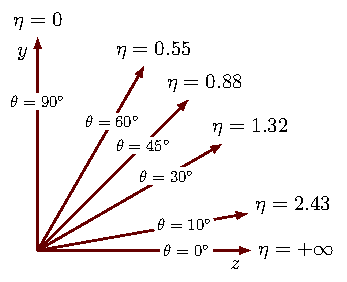
\includegraphics[width=1.\textwidth]{/home/bruno/org/PhD/Thesis/figures/detector/pseudorapidity_diagram.pdf}
\caption{\label{fig:pseudorapidity}Schmeatic of different pseudorapidity values and its polar angle \(\theta\) counterparts. Courtesy of Izaak Neutelings \cite{izaak_neutelings}.}
\end{figure}

\begin{figure}
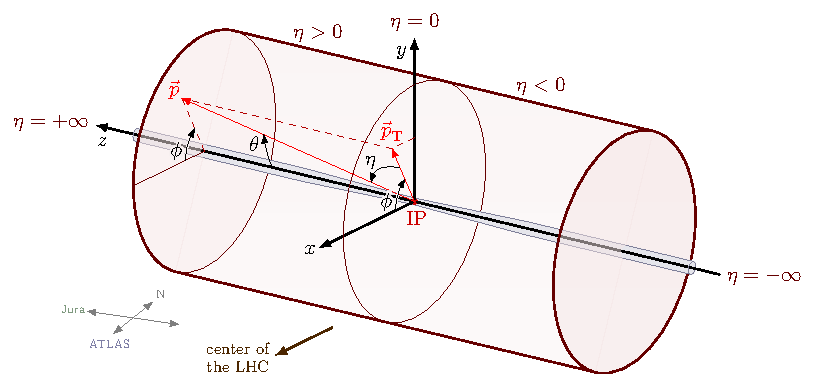
\includegraphics[width=1.\textwidth]{/home/bruno/org/PhD/Thesis/figures/detector/coordinates_left.pdf}
\caption{\label{fig:cords_cms}The coordinate system of the CMS detector, with the \ac{IP} at its origin. The relative geographical location of \ac{CMS} is also provided. Courtesy of Izaak Neutelings \cite{izaak_neutelings}.}
\end{figure}

\begin{figure}
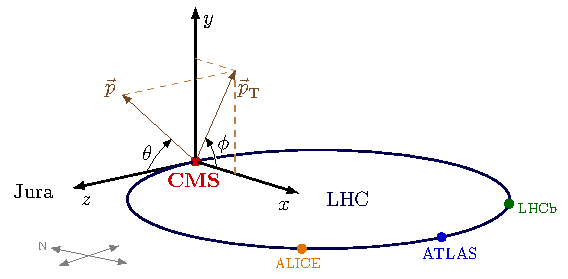
\includegraphics[width=1.\textwidth]{/home/bruno/org/PhD/Thesis/figures/detector/coordinates_cms.pdf}
\caption{\label{fig:cords_lhc}Schematic illustration of the standard coordinate system at the CMS detector, represented relative to the \ac{LHC} and the other three main LHC experiments. Courtesy of Izaak Neutelings \cite{izaak_neutelings}.}
\end{figure}
\subsubsection{Detector structure}
\label{sec:orgb475826}
They are designed to be versatile and capable of detecting a wide range of physics processes across various energies.
The CMS experiment was officially proposed in 1992 with the primary goal of discovering the \textbf{Higgs boson}.
Key to this objective were the channels \(H \rightarrow ZZ \rightarrow 4\ell\) and \(H \rightarrow \gamma\gamma\), which required an excellent electromagnetic calorimeter for effective electron and photon detection, with an energy resolution constant term equal to or less than \textbf{0.5\%}.

The architecture of the CMS detector is depicted in Figure 2.7.
It is a cylindrical apparatus with a length of \(21.6\,m\) and a diameter of \(14.6\,m\), comprising a central section known as the barrel, and two forward sections termed endcaps.
The precise demarcation between these regions varies according to the specific subdetectors in question.

To fulfill its versatile objectives, the CMS detector is outfitted with an intricate configuration of concentric detection layers.
Each layer is tailored to identify the various particles produced by collision events.
At the heart of this configuration, the pixel and strip tracker detectors, which encircle the interaction point, ascertain the location of collision vertices.
These detectors further delineate the trajectories and momenta of charged particles emanating from the collisions.
Encasing these trackers, the electromagnetic and hadron calorimeters gauge the energy imparted to their active material by electrons, photons, and hadrons, thereby facilitating precise energy quantification.
Enveloping the calorimeters, the CMS superconducting solenoid stands as the experiment's most salient characteristic.
The outermost layer is formed by the muon tracking chambers, which encompass the entire CMS volume.

Redundancy in the data from the various subdetectors is intentional, to maximize the accuracy of measurements for all types of final-state particles.
The subsequent sections detail the individual components of the CMS detector.
The application of this data in the offline reconstruction of physics objects is elaborated in Section 2.4.

\begin{figure}
\includegraphics[width=1.\textwidth]{/home/bruno/org/PhD/Thesis/figures/detector/cutaway_diagram.pdf}
\caption{\label{fig:ggtt_results}Cutaway 3D model of the CMS detector. This perspective makes visible all the sub-detectors at a glance. Taken from \cite{cms_cutaway_diagrams}.}
\end{figure}

A high-efficiency central tracking system was another fundamental requirement.
The tracker is essential for momentum measurement, particle identification, and vertex reconstruction.
To achieve precise momentum measurement, a powerful magnet was necessary, leading to the use of superconducting technology.
The CMS detector's structure and components are designed to meet these stringent requirements.
\subsection{The CMS trigger system}
\label{sec:orgd0e9bce}
\subsubsection{Level-1}
\label{sec:org62bc174}
\subsubsection{HLT}
\label{sec:org5e0816e}
\subsection{Offline identification and reconstruction of physics objects}
\label{sec:org9959dde}
\subsubsection{Particle-flow}
\label{sec:org2a0e7f0}
\subsubsection{Electrons}
\label{sec:org64854c5}
\subsubsection{Muons}
\label{sec:orgcb3aa17}
\subsubsection{Hadronic \(\tau\)'s}
\label{sec:org355cf4d}
\subsubsection{Jets}
\label{sec:org163f62d}
\subsubsection{Missing transverse energy}
\label{sec:org054e127}
\subsection{Monte Carlo generation}
\label{sec:org203e02e}
\begin{itemize}
\item Pythia: beams, hard-scattering, parton showering and hadronisation
\item jet matching and/or merging during hadronization
\item 
\end{itemize}
\subsubsection{Tunes}
\label{sec:org1c8906f}
The underlying event (UE) consists of the beam-beam remnants (BBR) and the particles that arise from multiple-parton interactions (MPI).
The BBR are what remains after a parton is scattered out of each of the two initial beam hadrons, while the MPI are additional soft or semi-hard parton-parton scatterings that occur within the same hadron-hadron collision \cite{CMS_Tunes}.

Underlying event (UE), defined as a accompanying activity to hard proton-proton scattering process,
is an unavoidable background to collider observables for most measurements and searches. The UE
activity is not constant on an event-by-event basis, so the contribution from UE cannot be subtracted.
However by using measurements sensitive to UE activity, the modelling of it in Monte Carlo (MC) event
generators is tuned. Multiple parton interactions (MPI) are one of the most important contributors to UE. \cite{hllhc_physics}

A set of QCD parameters is derived in different ways (WHICH ONES??) to precisely describe aspects of the UE, such as the modelling of the hadronization, the initial and final state radiation and the BBR.
A complex fitting procedure, using data collected by CDF and CMS at different energies is used, extracting the parameters known as CMS Pythia (CP) Tunes.
\subsubsection{Monte Carlo and data processing in \ac{CMS}}
\label{sec:org32733ff}
\begin{enumerate}
\item Data processing chain
\label{sec:orgc77bc61}
\begin{itemize}
\item @Follow section 2.5 of Alessandro's thesis@
\item create items with parton showering, hadronization, underlying event modelling\ldots{}
\end{itemize}
\item Pile-up production
\label{sec:org6b573d1}
There are two ways to produce samples with simulation of pile-up: premix and classical mixing \cite{pileup_production}.

Classical mixing implies a previous production of a \ac{MB} sample (with a datatier ``GEN-SIM'').
It contains the event at generator level and the interaction of the particles with the detector material.
For the generation of the sample with \ac{PU} (which happens in the \texttt{DIGI-RECO} step), a root \texttt{wmLHEGS/GS} request is digitized (namely the interaction of the particles with the detector material are used to simulate the signals in the detector cells) together with the PU sample.
The \texttt{DIGI-RECO} step needs the PU input dataset and the pile-up scenario, namely according to which distribution the pile-up should be simulated (and added to the root request).
Since the \texttt{DIGI} step is quite consuming and happens for both root request and \ac{MB} sample, classical mixing is generally more time and CPU consuming.

Premix is different because the \ac{PU} sample is digitized separately (at the time of the production of the premix library).
A \ac{MB} sample (datatier \texttt{GEN-SIM}) is produced in the same way as before, but it is here used for the production of a SingleNeutrino sample (basically nothing in the final state) which is interfaced with the simulation of the \ac{PU} according to a certain scenario and using the \ac{MB} sample.
The output of the SingleNeutrino sample is a \texttt{GEN-SIM-DIGI} sample (already digitized).
For root requests using premix \ac{PU} simulation, the \texttt{DIGI} step is run only on them, while the \ac{PU} simulation is added after this step.
Since the \texttt{DIGI} step is run only once, premix requests are much faster and less CPU consuming than classical mixing requests.
\end{enumerate}
\subsubsection{Improvements for the HL-LHC}
\label{sec:orgea09777}
\begin{itemize}
\item \cite{hllhc_physics}
\item quest for higher precision and accuracy, but also by practical issues, such as the need for generating very
\end{itemize}
large samples for the most abundant LHC processes, and for the efficient handling of the variations of
the input parameters needed in order to study uncertainties.
\begin{itemize}
\item cite MC generators: Herwig \cite{herwig1,herwig2,herwig3}, Pythia \cite{pythia1,pythia2}, Sherpa \cite{sherpa1}
\item from now up to the end of the \ac{HL-LHC} program we can anticipate continuous progress due to the \ac{LHC} running and accumulated data, which will provide continuous feedback to the theoretical work in the field. Developments in the following directions are to be expected: precision for inclusive observables, logarithmic accuracy, technical improvements for fast and efficient generation of events, and improvements in the modeling of hadronization and underlying event [pages 15 and 16 provide more details]
\end{itemize}
\subsubsection{Activities as Monte Carlo contact}
\label{sec:org0c819b9}
\section{Trigger primitives reconstruction for the HGCAL Level-1 trigger}
\label{sec:orgb2595e7}
\subsection{The High Luminosity LHC}
\label{sec:orgd5895cc}
\label{sec:hllhc}

The first phase of the \ac{LHC} has been running since 2010, spanning three independent data runs, the last of which, Run 3, is currently approaching its end of life, in the last quarter of 2025.
Phase-2 will soon follow, incorporating the brand new \ac{HL-LHC}, which will start taking data in 2029, extending \ac{HEP} studies well into the future (see \cref{fig:hllhc}) \cite{hllhc_evolution_paper1,hllhc_evolution_paper2}.
The \ac{HL-LHC} is designed to operate at a centre-of-mass energy of \SI{14}{\TeV}, achieving unprecedented instantaneous luminosities of \SIrange{\sim5e34}{7.5e34}{\per\cm\squared\per\second} \cite{hllhc}.
This is more than twice the \ac{LHC}’s current value.
These conditions correspond, in the ultimate HL-LHC configuration, to a \ac{PU} of up to 200, a fluence of up to \SI{1e16}{\nequiv\per\cm\squared}, and a \ac{TID} reaching \SI{2}{\mega\gray}.
For comparison, the \ac{LHC} currently brings \num{\sim 50} \ac{PU} interactions on average \cite{pileup_twiki}, a dose of the order of \SI{1e5}{\gray} and a fluence of \SI{\sim 1e15}{\nequiv\per\cm\squared} \cite{lhc_fluences} (see \cref{sec:lhc_design}).
An integrated luminosity of up to \SI{\sim 4}{\per\atto\barn} is envisaged to be collected over a period of around 10 years \cite{hllhc}, while current \ac{CMS} endcap calorimeters are designed to sustain a more modest value of up to \SI{500}{\per\femto\barn}.

\begin{figure}[htbp]
\centering
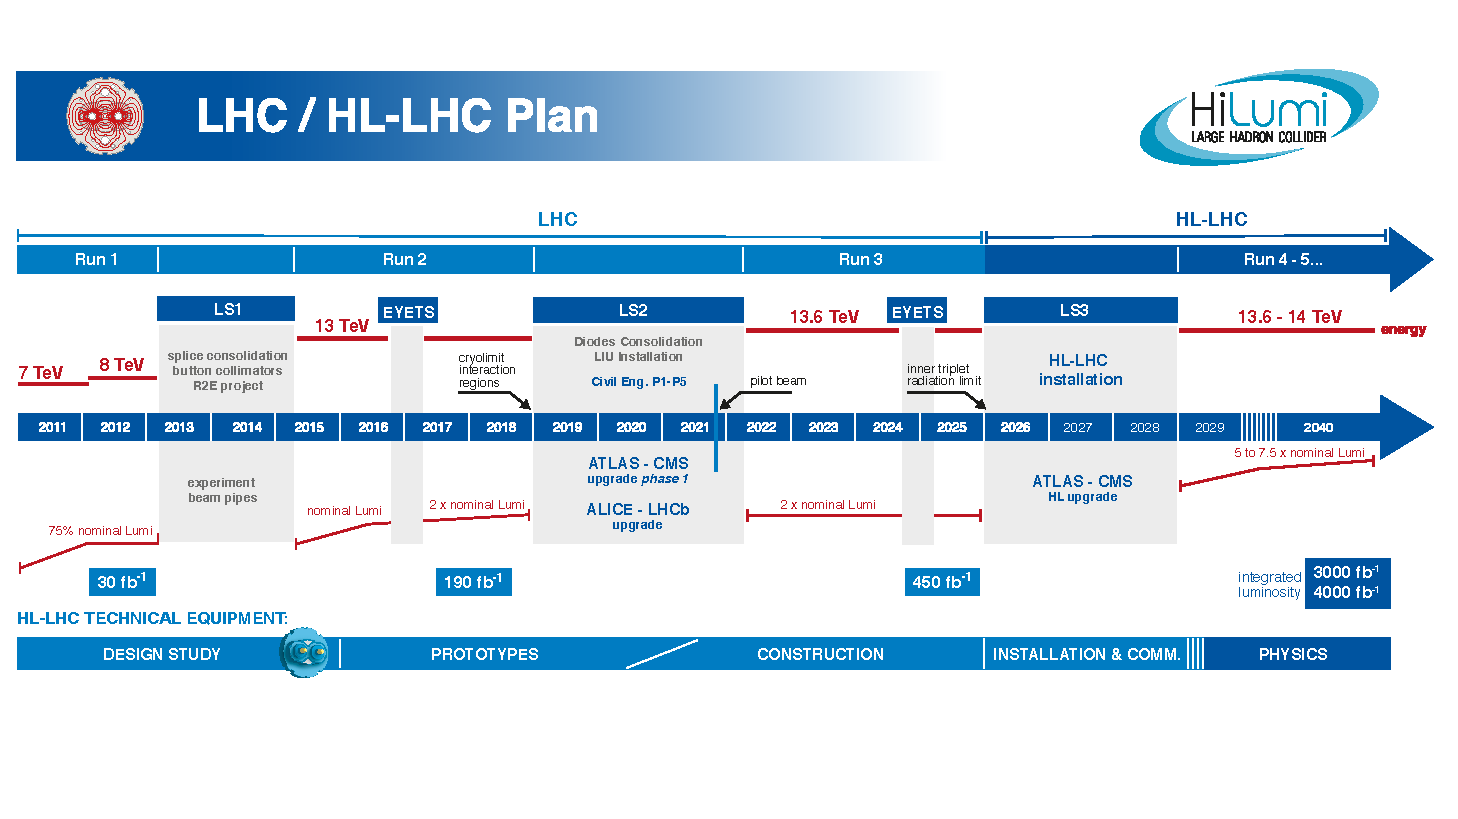
\includegraphics[width=1.\textwidth]{/home/bruno/org/PhD/Thesis/figures/hgcal/hllhc.pdf}
\caption{\label{fig:hllhc}The \ac{HL-LHC} project timeline. Run3 is currently on-going, and the \ac{HL-LHC} will start collecting data in 2029, following three years of \ac{LHC} shutdown for detector upgrades.}
\end{figure}

The operational scenario of the \ac{HL-LHC} is continuosly evolving, with some uncertainties still present.
Given past delays and current unknowns, it is still soon to definitely confirm current operational plans.

\begin{figure}
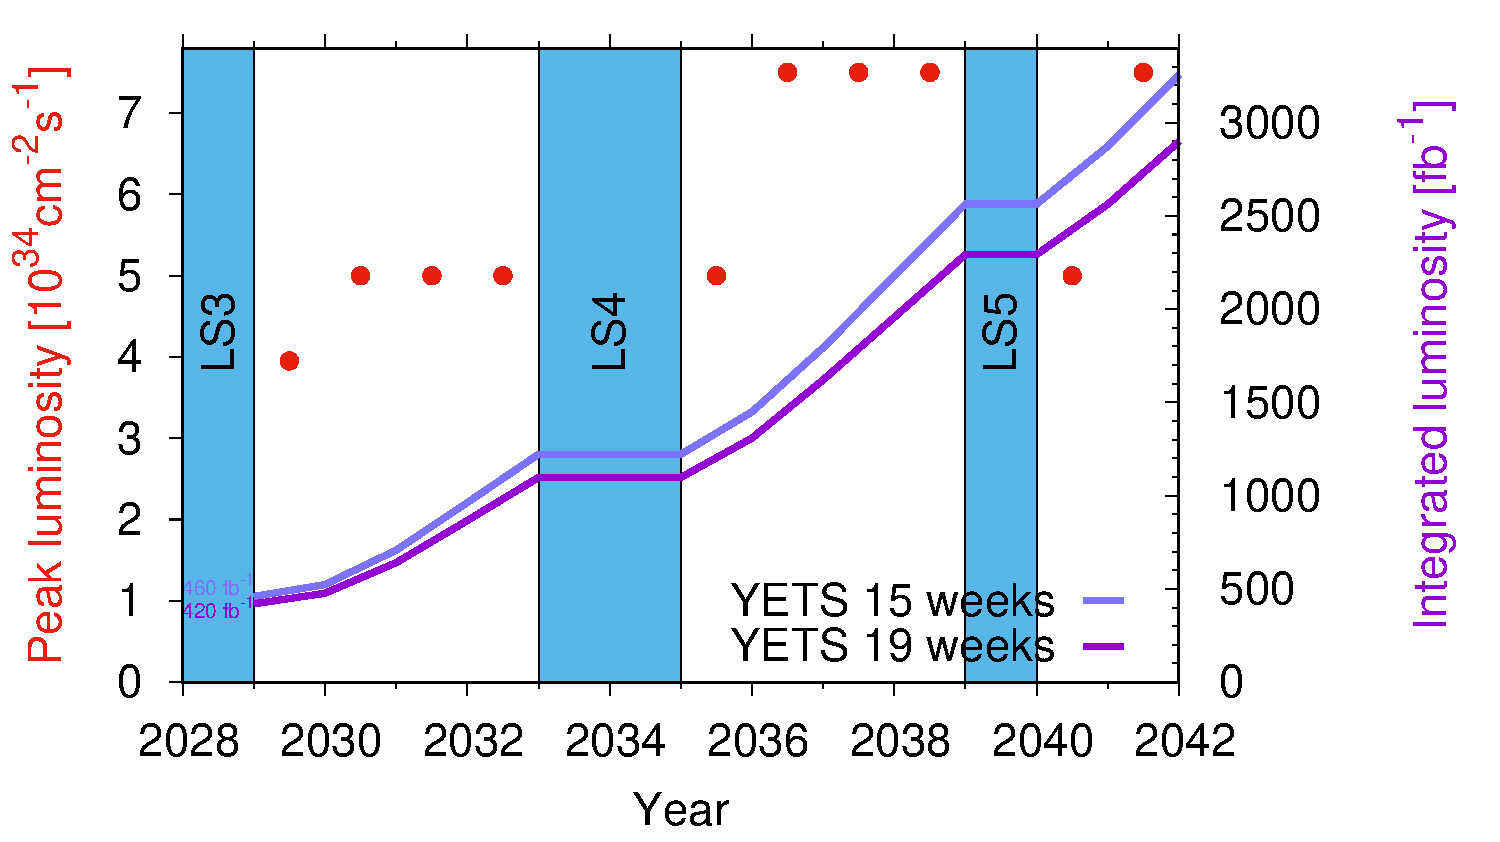
\includegraphics[width=1.\textwidth]{/home/bruno/org/PhD/Thesis/figures/hgcal/lhc/lumi_evolution_hllhc.pdf}
\caption{\label{fig:lumi_plans_hllhc}Planned peak and integrated luminosities during the \ac{HL-LHC}. Three data-taking runs are foreseen, interspersed by three \acp{LS}. Two scenarios with different \ac{YETS} durations are shown, where shorter stops have the potential for significant integrated luminosity increases. The schedule was last updated in January 2022. Taken from \cite{hllhc_evolution_paper2}.}
\end{figure}
\subsubsection{Physics motivation}
\label{sec:orgb607cd0}
\label{sec:hllhc_physics}

A more powerful \ac{LHC} will increase the accurancy of current measurements and enhance the sensitivity to rare processes through both direct and indirect searches which occur below the current sensitivity level, and with more challenging signatures.
The \ac{HL-LHC} is expected to provide high-precision measurements of the \ac{SM}, particular in Higgs physics: the Higgs boson (H) self-coupling, via direct and indirect measurements (see \cref{sec:dihiggs}), higgs couplings, flavour physics, BSM

A virtuous cycle often takes place between data collection and improvements in simulation and theory calculations.
In the following we provide a brief and necessarily incomplete overview of some of the physics motivations to build the \ac{HL-LHC}.
A detailed description is out of the scope of this work.


\paragraph{EW processes}

The increase in luminosity provided by the \ac{HL-LHC} will provide a significant boost in sensitivity to measurements of (small) electroweak couplings, especially when dealing with low cross-section processes.
This notably applies to W mass \(\mw\) and weak mixing angle \(\thw\) measurements, but also to \ac{VBF}, \ac{VBS}, and tri-boson production measurements.
\num{\sim 2e6} W boson events will be collected per week, leading to a statistical sensitivity of about \SI{10}{\MeV} for the \(W\) mass, and significantly lower for cross-section measurements.
The added luminosity might also help solving the tension between old \(\theta_{W}\) measurements performed by \ac{LEP} and Tevatron, adding to the recent \ac{CMS} result \cite{weak_mixing_angle_cms}, which agree with the \ac{SM}, just as previous \ac{LHC}-hosted measurements.
Concerning \ac{VBF} and \ac{VBS} processes, despite the overall lower cross-section, of about one order of magnitude with respect to the \ac{ggF} production, the presence of additional hard and forward jets enables a very significant reduction of the multijet background.
This is particularly true for large rapidity separations \(\Delta \dijetrap \gtrsim 4.5\) and di-jet invariant masses
\(\dijetmass \gtrsim \SI{700}{\GeV}\), where \ac{VBF} production dominates over \ac{ggF}.
In \ac{VBS}, measurements of longitudinal scattering of two \(V\) (\(V=W,Z\)) is particularly enticing, as it is still unknown whether the Higgs alone can avoid a divergent behaviour of the scattering amplitude at high energies, violating unitarity \cite{vbs2}.
The longitudinal component of the \(V\) bosons is in particular tightly connected to the Higgs mechanism and \ac{EWSB}, since massless particles only have transversal components.
However, differential measurements of gauge boson polarization is harder given the reduced cross-section of the longitudinal-only components.
Would unitarity be violated, particle probability would no longer be conserved: the calculated number of \(V\) pairs produced in the interaction would exceed the incident flux \cite{thomson}.
There is also the possibility for the longitudinal components of the \(V\) bosons to be strongly coupled at \SI{\sim 1}{\TeV} center-of-mass energies \cite{vbs1}, allowing for instance the formation of resonance states in technicolor models.
\ac{VBS} also forms the ideal field for anomalous gauge couplings measurements, especially quartic couplings.
Finally, even rarer tri-boson processes (\(\sigma\)\SI{\sim 0.1}{\pico\barn}) brings an extra handle on \ac{SM} testing.

\paragraph{Strong interactions}

The \ac{HL-LHC} will enable an increase in the kinematic reach for jet and photon production.
This will in turn reduce the associated experimental uncertainties, improving \ac{PDF} modeling.
High-\(\pt\) b-jets are sensitive to higher-order corrections, parton shower modeling and \acp{PDF}.
Therefore, investigating the b-jet contribution to the total jet cross section enables to test the available theoretical predictions.
The shape of the distributions of jets of various flavours will also be known with a higher precision, especially in the tails.
On the photon side, diphotons with high invariant mass are ideal probes to test the \ac{SM} and search for \ac{BSM}. In particular, prompt photons do not interact with other final state particles, enabling a precise study of \ac{QCD} \cite{diphoton_cdf}.
The \ac{HL-LHC} will enable a more precise knowledge of photon related cross-sections.
For the first time, the \ac{HL-LHC} will make possible the measurement of quantum correlations between partons in the proton by precisely studying differential distributions.
This brings an improvement in \ac{DPS} modeling, which has been so far very limited.
\ac{DPS} can be as relevant as the single proton scattering for same-sign \(WW\) final states involving \(b\bar{b}\) or \(c\bar{c}\) quark pairs.

\paragraph{Top physics}
The heaviest particle in the \ac{SM} plays an important role in \ac{EWSB} and in \ac{BSM} searches.
With the \ac{HL-LHC} we will be able to improve the precision of the \(\mt\) measurement, and to study \(t\bar{t}\) differential distributions in more detail, reaching \(\mtt\sim 7\,\si{\TeV}\) and \(\pt\sim 2.5\,\si{\TeV}\).
This will provide benefits for \ac{PDF} measurements.
One can also explore \ac{BSM} for \(\mtt > 7\,\si{\TeV}\) due to the low \ac{SM} background.
An interesting link might be drawn between the results of \ac{LHCb} and \ac{ATLAS}/\ac{CMS}, given the increase in \(\eta\) reach up to \num{\sim 4}.
There will be as well the possibility to observe the rare \(t\bar{t}t\bar{t}\) production for the first time, despite its small cross-section of \(\mathcal{O}(10)\,\si{\per\femto\barn}\).
\(t\bar{t}t\bar{t}\) can be used to constrain some of the Wilson coefficients associated to \ac{EFT} dimension-6 operators, to further study the top Yukawa coupling constrain, including its magnitude and \ac{CP} properties, since it can occur via de mediation fo a Higgs boson \cite{tttt}, and even to assess the presence of the non-\ac{SM} top quark dipole moment.

\paragraph{Forward physics}

Assuming concepts similar to the current \ac{CTPPS} \cite{ctpps_tdr} and \ac{AFP} \cite{afp_tdr} detectors are extended in the \ac{HL-LHC} phase, \ac{CEP} \(pp \rightarrow p\,(\gamma\gamma\rightarrow X)\,p\) phenomena, among which light-by-light scattering (\(X = \gamma\gamma\)), will be further explored \ac{CEP}.
Other processes include, for instance, \(X = \mu\mu,\,\tau\tau,\,Z,\,H,\,WW,\,ZZ\), and enable the study of anomalous gauge couplings and the magnetic moment of the \(\tau\), among other studies \cite{ctpps_varela,ctpps_pitt}.
\ac{CEP} processes carry particular interest since they bring production of charged particles initiated only by photons, into what amounts to using the \ac{LHC} as a \(\gamma\gamma\) collider.
In parallel, a whole plethora of \ac{QCD}-related measurements can be performed in \acp{CEP}.
The \ac{HL-LHC} will push \ac{CEP} processes to higher masses and lower cross-sections, increasing their discovery potential.


\paragraph{Higgs boson pairs}

\cref{fig:hh_nonres_projections} allows the comparison of early \run{2} results with current full \run{2} upper cross-section limits.
An improvement of a factor of \num{\sim 7} was obtained, much above what a naive luminosity scaling would provide, given the four-fold increase in collected data.
The improvement over the luminosity baseline is due to improvements which span multiple areas, such as trigger, identification, and reconstruction algorithms, but also to the increase of explored finals state channels, made possible by the gradual increase in available number of events.

@150 Million Higgs and 120k HH@
One hundred thousand Higgs boson pairs are expected to be produced during the \ac{HL-LHC} phase.
This will enable the most precise measurement of the triple and quartic Higgs couplings ever, with the possibility of observing the former for the first time, most likely after combining \ac{CMS} and \ac{ATLAS} datasets.
The precision of \ac{EFT} couplings will also benefit from the increased number of events.
The sensitivity will in general benefit from the extension of the phase-space, which adds relevance to yet unexplored HH production modes and decay channels, to be added to future multi-channel combinations \cite{higgs_10_years}.
At present, none of the analyses used to search for the production of Higgs boson pairs is statistically limited \cite{andre_david_higgs_ten_years}.
However, \ac{ggF} theory uncertainties might soon become important.

A series of new techniques should improve results even further, starting from \run{3} and extending into the \ac{HL-LHC}, including new machine learning techniques or better estimates of \ac{QCD} multi-jet background.
The usage of \ac{PNet} \cite{particle_net} for \(\tau\)-initiated jets and the application of transformer technology to jet tagging \cite{particle_transformer} are expected to boost HH sensitivity.
Additionally, an improved trigger strategy has been implemented, considering both data scouting and parking \cite{parking_scouting_run3_cms}, and including \ac{PNet} b-tagging and \(\tau\)-tagging at trigger level.
We also expect that some HH analysis might benefit from the inclusion of synthetic datasets \cite{zz_zh_bbbb}.
As discussed in \cref{sec:indirect_searches}, indirect searches can very significantly contribute to an increase in \(\lh{3}\) sensitivity.
In conclusion, the next decade looks extremely promising in what concerns HH coupling measurements.
Such measurements would deeply impact a whole range of available theoretical frameworks, such has flavour models (with \acp{2HDM} as an example) and models implying a \ac{EWPT} (see Section \cref{sec:ewpt}).
If we also take a positive and historical stand, considering how \ac{LHC} experiments have consistently surpassed initial estimates, we can surely hope to be soon able to assess the way the Higgs particle interacts with itself.

\begin{figure}[htbp]
\centering
\includegraphics[width=.5\textwidth]{/home/bruno/org/PhD/Thesis/figures/intro/hh_nonres_projections.pdf}
\caption{\label{fig:hh_nonres_projections}Evolution of the expected and observed upper limits on the HH production cross-section. The figure compares results from early \ac{LHC} \run{2} data (\SI{35.9}{\invfb}) with full \ac{LHC} \run{2} data (\SI{138}{\invfb}), and with projections for the \ac{HL-LHC} (\SI{3000}{\invfb}). At the end of the \ac{HL-LHC} it should be possible to challenge the \ac{SM} prediction (red line) with the result of a combined analysis of multiple final states. Taken from \cite{higgs_10_years}.}
\end{figure}
\subsubsection{Detector ugrades}
\label{sec:orgf13993f}
\label{sec:hllhc_detector_upgrades}

\paragraph\{\ac{LHCb}\}

mention VELO

\cite{lhcb_hllhc_tdr,lhcb_hllhc_interest}

\paragraph{SHiP}

\paragraph{LBNF/DUNE}

\paragraph{ALICE}
\subsubsection{Future CMS subdetectors}
\label{sec:orgfe6fb26}
\label{sec:hllhc_future_subdetectors.org}
\begin{enumerate}
\item Pixels
\label{sec:orgfeb6f77}
\begin{itemize}
\item New Layer 1 at 29mm from the beamline
\end{itemize}
\item Muons
\label{sec:org550ba2c}
\item HCAL
\label{sec:org7f966b0}
\begin{itemize}
\item in HCAL hybrid photodiodes were replaces by SiPMs (in Run1)
\item HCAL brings new depth and timing information
\end{itemize}
\item Bril
\label{sec:org184152f}
\begin{itemize}
\item lumi measurements are challenging
\item uncertainty of 1.4\% in 2022
\end{itemize}
\item L1
\label{sec:orgef400e8}
\begin{itemize}
\item Folded event building in Run3
\item GPUs in Run3 (and replace CUDA by Alpaka)
\item using PNet in HLT
\item special paths for LLPs
\item scouting
\end{itemize}
\end{enumerate}
\subsection{The High Granularity Calorimeter}
\label{sec:org0647040}
\label{sec:hgcal_intro}

Running conditions during the data collection of \ac{HL-LHC} will take place in a environment much harsher and crowded when compared to the \ac{LHC}.
This is particularly true for the \ac{CMS} endcap regions, given the large radiation levels expected closer to the beam axis.
At the same time, the forward \ac{ECAL} and \ac{HCAL} were designed to sustain an integrated luminosity of \SI{500}{\invfb}.
Given the \num{\sim 6} to \num{8} times larger luminosities expected during the entirety of the \ac{HL-LHC} period, a drastic degration of the physics performance seems unavoidable \cite{hgcal_technical_proposal}.
Unfortunately, scintillation-based solutions are very sensitive to ionizing radiation.
The formation of color centres during irradiation has already lead to a stark \(\eta\text{-dependent}\) reduction of the transparency of existing endcap \ch{PbWO4} crystals, often by values above 90\%.
Despite the possible recover from the opaqueness caused by photons, through spontaneous annealing, or thermal annealing at \SI{200}{\celsius} \cite{annealing_calorimeter}, irreversible damage is caused by fast hadrons, mostly charged pions of \SI{\sim 1}{\GeV} \cite{wigmans,wigmans2}.
The endcap calorimeters would become unusable during the \ac{HL-LHC}, and negative effects would be evident almost from the start (see \cref{fig:lumi_plans_hllhc}).

The CMS experiment thus foresees the complete replacement of its endcap calorimeters, introducing the challenging \ac{HGCAL} project \cite{hgcalTDR} (see \cref{tab:HGCALparameters}).
The \ac{HGCAL} will be a sampling calorimeter, with fine transverse and longitudinal granularity, capable of fully exploiting the physics events produced under the expected extreme radiation conditions.
It will proeminently feature \ac{Si} as active material in the regions closer to the \(pp\) interaction point, and thus more impacted by incoming radiation.
This approach departs from others more established technologies, for instance the use of liquified noble gases, as done in \ac{ATLAS}.
\ac{Si} was chosen for its ability to cope with fluences 50\% higher than the ones expected by the end of Phase-2.

The proposed novel design includes an \ac{EM} electromagnetic section of silicon sensors as active material in the first \num{26} layers, as one can see in \cref{fig:hgcal_side_view}.
In total, \ac{HGCAL} has \num{\sim 6} million \ac{Si} sensors, or channels, with three different thicknesses of \num{300}, \num{200}, and \SI{120}{\micro\meter}, ordered by the fluence impinging on them.
In order to optimise the charge collection and reduce the leakage current, it is advantageous to use thinner sensors in the regions of higher fluence.

Sensors will be split in two different density regions, depending on their active area size.
The \emph{high density} region comprises \SI{0.52}{\centi\meter\squared}, \SI{120}{\micro\meter} thick cells, and is located closer to the beam axis.
Instead, the \emph{low density} region, located at \(|\eta| \lesssim 2.15\) (\(R \lesssim 70\si{\centi\meter}\)), will be made of \SI{1.18}{\centi\meter\squared} active sensors, with thicknesses of \num{300} or \SI{200}{\micro\meter}, depending on their location.
Their physical layout can be inspected in \cref{fig:hgcal_side_view}.

The sensors are arranged within \SI{8}{\inch} hexagonal \ac{Si} modules, which are mounted on one side to a baseplate, and on the other side to the hexaboard containing the front-end electronics and the \ac{PCB}. The baseplate is composed of CuW in the \ac{CE-E}, contributing to the \ac{CE-E} absorber,

\begin{figure}
\begin{center}
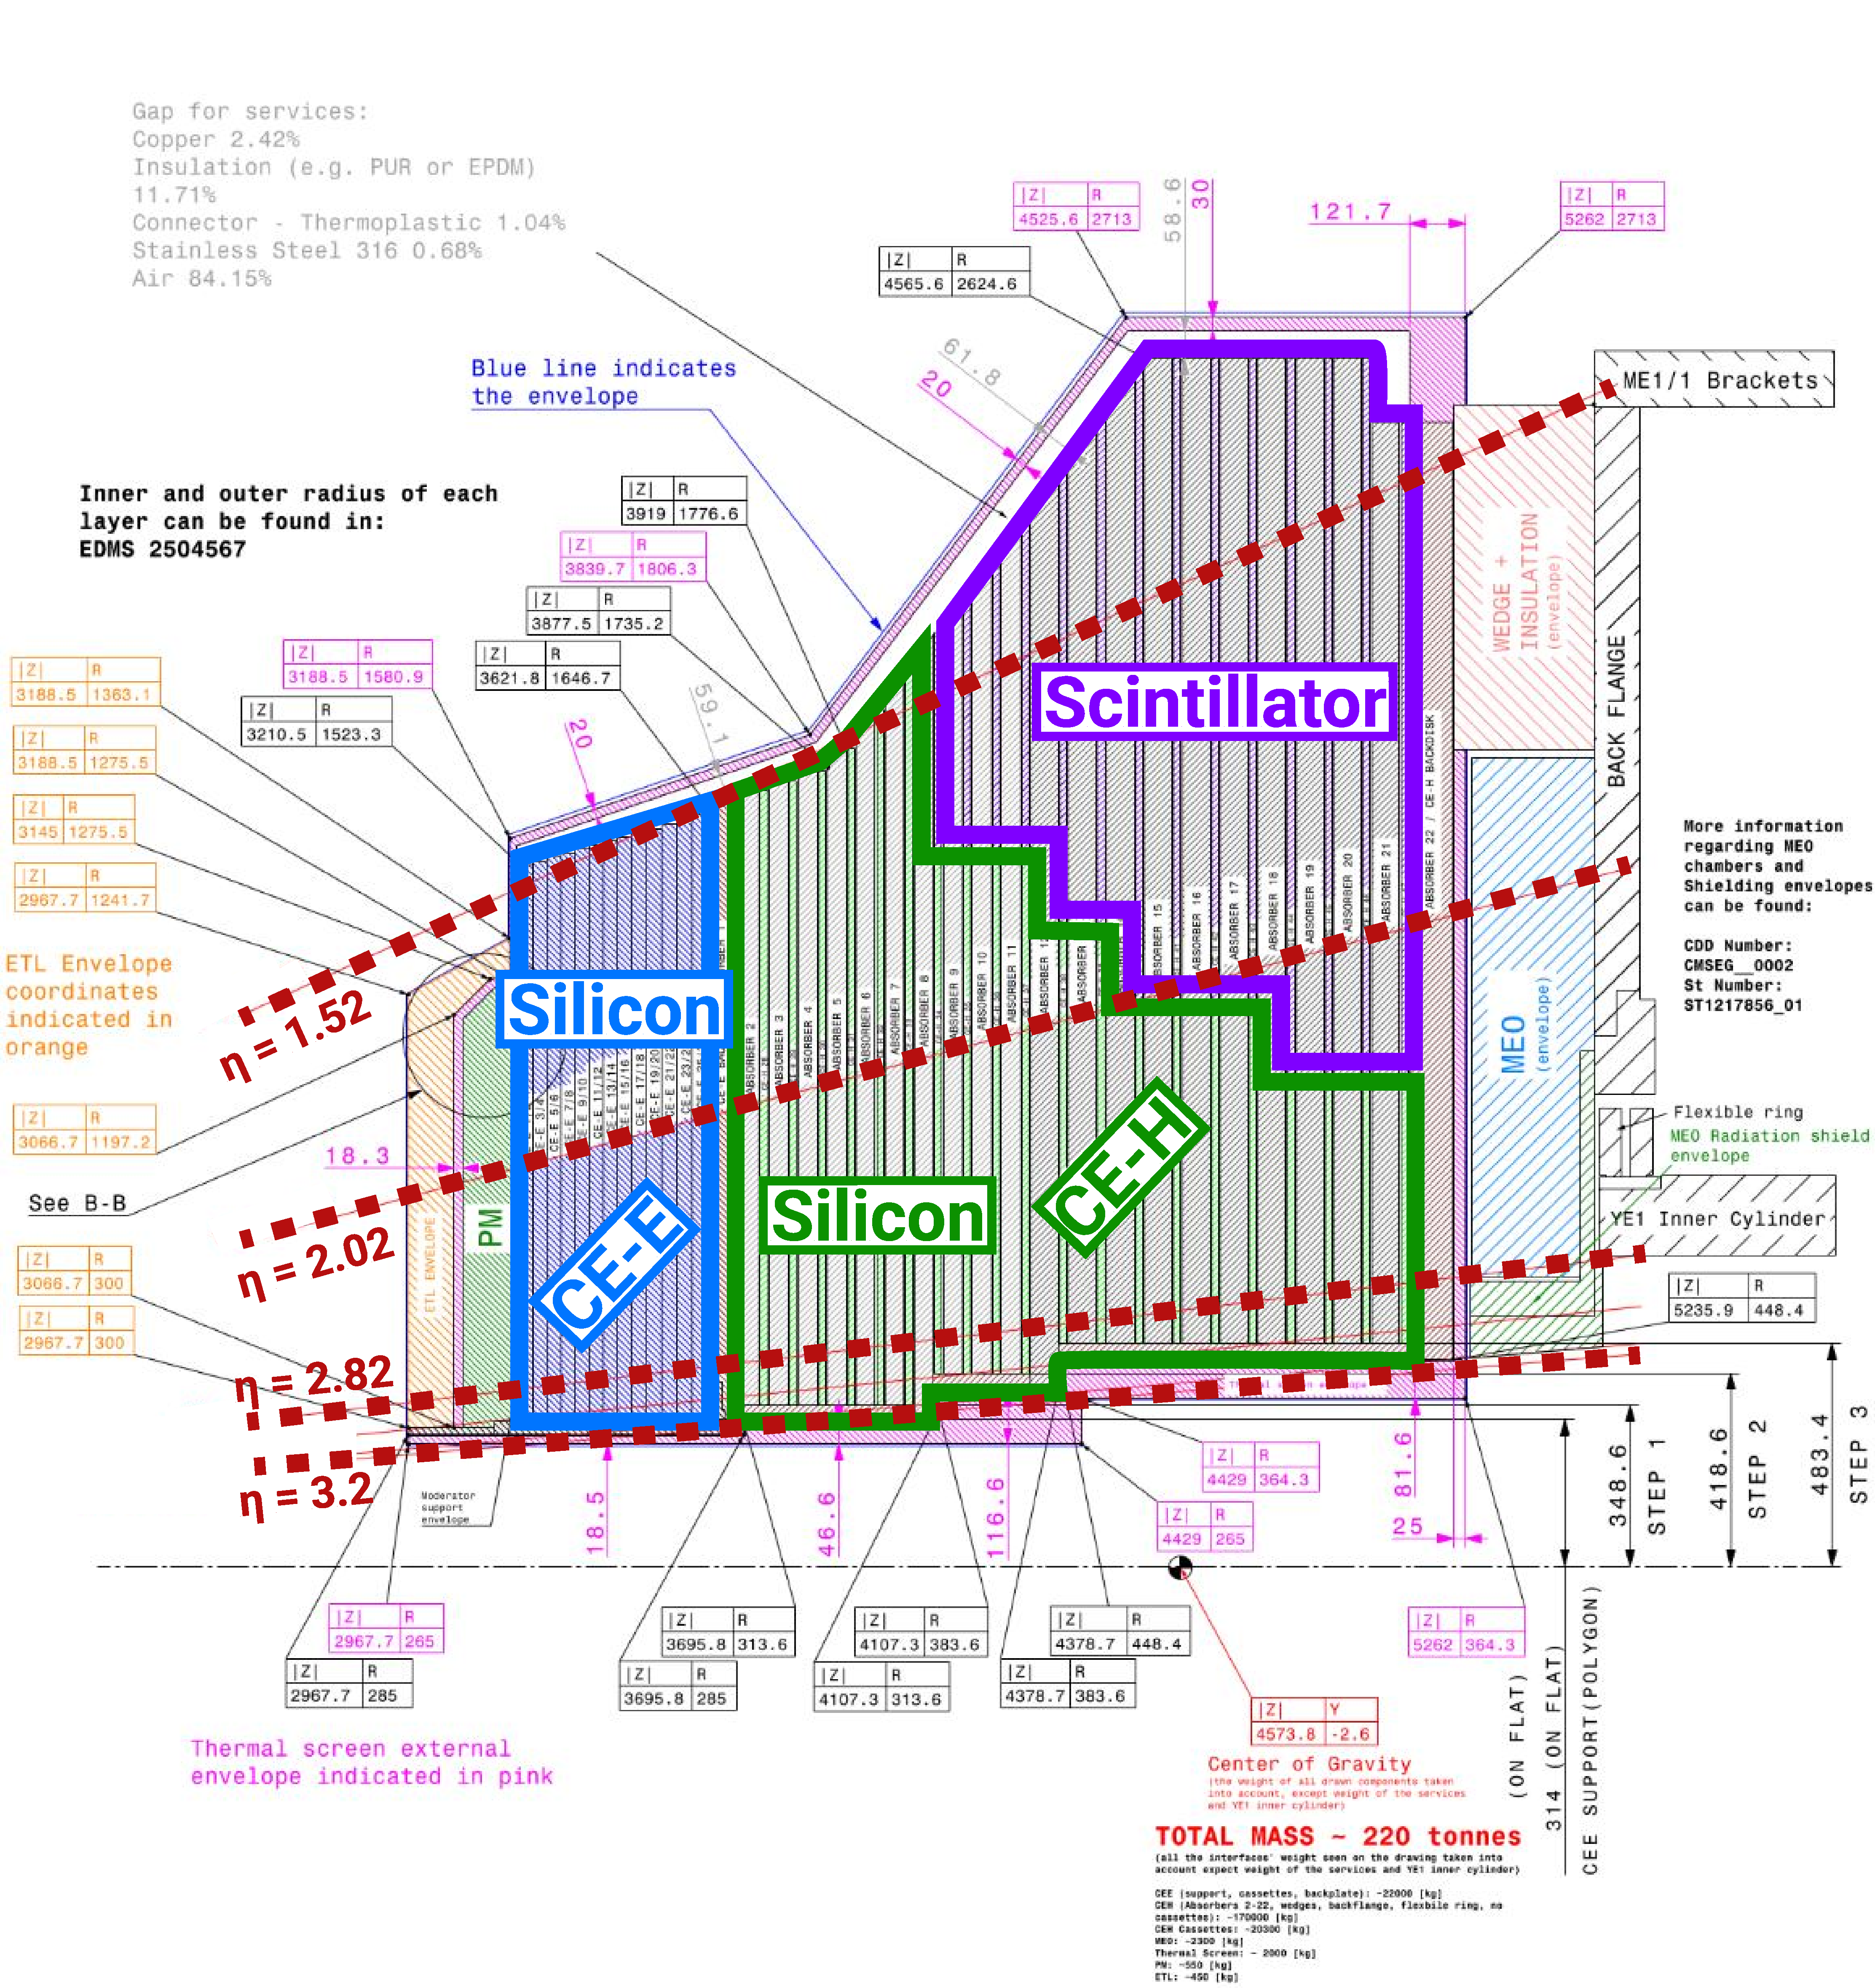
\includegraphics[width=1.\textwidth]{/home/bruno/org/PhD/Thesis/figures/hgcal/HGCALSideView.pdf}
\end{center}
\caption{\label{fig:hgcal_side_view}The longitudinal profile of the positive endcap \ac{HGCAL} in its latest design version. The first \num{26} layers, in blue, refer to the \ac{CE-E}. The \ac{CE-H} follows, in green, and some hybrid layers lie deeper in the calorimeter, where purple refers to the region with plastic scintillator tiles. The active material alternates with absorber material, which varies according to the detector location, as described in the text. Adapted from \cite{hgcal_web}, which is partially based on \cite{hgcalTDR}.}
\end{figure}

\begin{figure}
\begin{center}
\includegraphics[width=1.\textwidth]{/home/bruno/org/PhD/Thesis/figures/hgcal/DoseAbsorbedHGCAL.pdf}
\end{center}
\caption{\label{fig:dose_abosrbed_hgcal}Distribution of the absorbed dose over the \ac{CMS} detector after an integrated luminosity of \SI{3}{\atto\barn}. Used \ac{CMS} \texttt{FLUKA} geometry, version 3.7.0.0. Taken from \cite{hgcalTDR}.}
\end{figure}


The extremely high granulairty will enable particle identification and high resolution measurements of the position, energy and time of high-energy collision products.
The granularity is such that \ac{HGCAL} will be the first calorimeter ever able to perform tracking.
The high segmentation also enables the precise measurement of narrow and merged jets, and of \ac{PU} energy, for instance.

\cite{bruno_chep23}













There, \ac{Si} sensors organized in hexagonal modules act as active material, in order to sustain the expected radiation.
\cite{refCUDA1}

A \ac{HAD} section comprises \num{8} silicon-only layers followed by \num{14} hybrid layers composed of both silicon and \ac{Sci} plastic tiles, where the scintillation light is read out by \acp{SiPM}.
Both sections are interleaved with absorber layers.
\ac{HGCAL} will comprise \SI{\sim 620}{\meter\squared} of \ac{Si} and \SI{\sim 400}{\meter\squared} of plastic scintillators for a total of, respectively, \num{\sim 1} million and \num{\sim 240} thousand channels.
Three subdetectors form HGCAL’s hybrid detection technology: the first \num{28} layers made exclusively of silicon (\ac{CE-E}) and the silicon and scintillator parts of the hadronic section (CE-HSi and CE-HSci).

The following 21 layers, comprising the \ac{HAD} section, are split into 8 \ac{Si}-only layers followed by 14 hybrid layers, with \ac{Si} closer to the beamline and cost effective plastic scintillator at lower \ac{eta} values (see \cref{fig:hgcal_side_view})
\begin{enumerate}
\item Sensor thicnkess
\label{sec:orgca4b33a}
radiation induced traps in the bulk silicon significantly reduce the charge collected.
In addition, the sensor leakage current linearly with fluence, resulting in increased noise and, combined with the very high
bias voltages, leads to substantial power dissipation within the sensors themselves.
These observations motivated the investigation of thinner sensors. \cite{hgcalTDR}
\item Satisfy requirements
\label{sec:org49e7590}
The new calorimeter addresses many of the requirements imposed by the \ac{HL-LHC}:
\item Neutron moderator
\label{sec:org2c53e9d}
Despite \ac{Si}'s radiation hardeness, fast enough photons and hadrons can cause damage in the sensors.
Starting by the dominant ``soft'' damage, two negative effects can occur.
The first type, bit flips, can occur whenever a high energy track passes closer to a capacitor.
If the latter is empty, the original ``0'' might be read as a ``1''.
This type of errors can be reversed by software corrections and/or redundancy, or simply by resetting the state of the sensor.
The second type, namely the creation of charge traps between the valence and conduction bands, has the effect of lowering the resolution of the semiconductor device.
Soft damage can be usually reversed by temperature annealing.
The so-called displacement damage, instead, occurs when a high energy particle, like a photon, neutron or proton knocks an atom from its lattice site. Eventually the resulting vacancies stabilize, creating long-lasting defects.
To avoid the deterioration of the crucial (and expensive) \ac{Si} sensors, the \ac{PM} neutron moderator will be added in front of the \ac{CE-E}, to reduce the number of fast neutrons coming from the tracker \cite{calorimetry_fabjan,radiation_damage_silicon2,radiation_damage_silicon}
\item Table parameters
\label{sec:orgdb86575}
\begin{table}[!h]
\centering
\begin{tabular}{c|c}
Parameter & Value\\
\hline
\(\eta\) coverage & \(1.5 \lesssim \eta \lesssim 3.0\)\\
Area of \ac{Si} sensors & \SI{620}{\meter\squared}\\
Area of \ac{Sci} tiles & \SI{400}{\meter\squared}\\
Endcap radial length & \SI{2.3}{\meter}\\
Endcap longitudinal length & \SI{2}{\meter}\\
Endcap weight & \SI{215}{\tonne}\\
Temperature & \SI{-35}{\celsius}\\
Number of modules & \num{30000}\\
Number of \ac{Si} channels & \num{6000}\\
Number of plastic tile boards & \num{4000}\\
\end{tabular}
\caption{\label{tab:HGCALparameters}Defining HGCAL properties.}

\end{table}
\item Table parameters 2
\label{sec:orgeb439c6}
\begin{table}[!h]
\centering
\begin{tabular}{c|c|c|c}
Tickness [\si{\micro\meter}] & 120 & 200 & 300\\
\hline
Cell size [\si{\centi\meter}] & 0.52 & 1.18 & 1.18\\
Expected fluences [\(\times10^{15}\) \unit{\nequiv\per\cm\squared}] & \numrange{2}{7} & \numrange{0.5}{2.5} & \numrange{0.1}{0.5}\\
\end{tabular}
\caption{\label{tab:Si_sensors_parameters}Features of the silicon sensors in the layers deploying only silicon sensors. The silicon cell size defines two regions, namely the high-density and low-density region.}

\end{table}

\begin{figure}
\includegraphics[width=1.\textwidth]{/home/bruno/org/PhD/Thesis/figures/hgcal/HGCAL3DView.pdf}
\caption{\label{fig:hgcal_3d_view}Schmetic 3D view of one endcap of the \ac{HGCAL}. Different detector structural layers can be seen, such as the \ac{CE-E} and \ac{CE-H} calorimeters, the \ac{ETL} located just in front of the \ac{CE-E}, and some sections required for structural reasons. The \ac{PM}, or neutron moderator, reduces the number of neutron coming from the tracker. The two dashed lines give a rough idea on the location of one pair of cooling supply and return tubes, which are connected to the layers, and are placed every \SI{30}{\celsius}. The picture on the right provides a side view of the same endcap. Adapted from \cite{hgcalTDR}.}
\end{figure}
\item Diamond semdiconductors
\label{sec:orgf568b6d}
\begin{itemize}
\item Although the specific ionization in diamond detectors is around three times smaller
\end{itemize}
than in silicon, larger detector thickness, small dielectric constant, high break down
voltage and negligible leakage current make them the most viable replacement for
silicon in the highest radiation fields \cite{calorimetry_fabjan}
\begin{itemize}
\item altneratives to silicon in niche applications are silicon carbide, GaAs and GaN.
\end{itemize}
\item Reconstruction code
\label{sec:org4667400}
Given its location and number of active sensors, data rates of \SI{\sim 100}{\tera\byte\per\second} are expected.

This requires the development of reconstruction code capable of fully exploiting the increased granularity under the expected extreme conditions.
The biggest contributor to CPU usage is event reconstruction, of which currently ∼5\% is
used by HGCAL [5]. CMS plans to port part of its reconstruction to Graphics Processing
Units (GPUs), which represent one of the most promising hardware accelerator technologies on
the market. GPUs are a key element when one considers taking advantage of heterogeneous
architectures available on traditional and High-Performance Computing grid sites, including the
upgraded Worldwide LHC Computing Grid. GPUs also promote the development of algorithms
with better computing performance, and profit from a potentially favourable cost when compared
to CPUs, per unit capacity. CMS is planning to adopt a heterogeneous High Level Trigger (HLT)
farm already in Run 3 (2022–2025), where ∼30\% of the workflow will be offloaded to GPUs (50\%
and 80\% by the end of Run 4 and 5, respectively) [6]. 

The reconstruction model envisioned for \ac{HGCAL} is intended to be fast and flexible, comprising a sequence of modules/stages which transform raw data into physics objects.
After the initial generation, simulation, digitization [5]
and calibration steps, energy deposits (hits) are clustered by CLUE, a fully-parallelizable density-
based clustering algorithm [8], in order to form two-dimensional objects. In a nutshell, CLUE
assigns an energy density and a separation distance to all hits, which are later used to classify
each hit as either a seed, a follower (based on the hit’s nearest highest density), or an outlier.
Clusters are built by traversing the tree of followers of each seed, assigning the index of the
seed to all its followers. This work includes the calculation of the cluster energy and cartesian
positions, which are computed in the device (section 3.1). In addition, a heterogeneous approach
for navigating through the detector’s geometrical/topological information is devised and used
within CLUE (section 3.2).

\begin{figure}
\begin{center}
\includegraphics[width=1.\textwidth]{/home/bruno/org/PhD/Thesis/figures/hgcal/layer_structure.pdf}
\end{center}
\caption{\label{fig:hgcal_side_view}Representation of the silicon sensors with two possible cell sizes. layout of a layer where only silicon sensors are present. The radial changes in darkness of colour indicate the different silicon thickness: 300, 200, and 120 μm. The solid black line marks the boundary between the high-density and low-density region. The succession of green and yellow colours delimit the 60◦ cassettes. The right half-circle shows the layout of a layer where both silicon sensors and scintillators are present. The blue lines in the scintillator part and the red lines in the silicon part delimit the \SI{30}{\degree} cassettes. Taken from \cite{tarabini_thesis}.}
\end{figure}

\begin{figure}
\begin{center}
\includegraphics[width=.5\textwidth]{/home/bruno/org/PhD/Thesis/figures/hgcal/CEEcass.pdf}
\end{center}
\begin{center}
\includegraphics[width=.5\textwidth]{/home/bruno/org/PhD/Thesis/figures/hgcal/CEEcass.pdf}
\end{center}
\caption{\label{fig:hgcal_long_structure}Longitudinal structure of a fundamental unit of the \ac{CE-E}. Each unit comprises two sampling layers. ADD HAD one!!!!}
\end{figure}


Wigmans \cite{wigmans2,wigmans}
\end{enumerate}
\subsubsection{Random}
\label{sec:orgb36b9c8}
\begin{itemize}
\item \cite{hlttdr} (I wrote Section 12.3)
\item Maximize granularity to fully exploit CMS Particle Flow reconstruction
\item fine lateral granularity for two-shower separation + narrow jets observation and minimize pileup contribution to energy measurement
\item fine longitudinal granularity for electromagnetic energy resolution (H->gg for instance), pattern recognition and discrimination against pileup
\item Fully utilise timing, firs time in calorimetry High-precision timing is considered one of very few options to mitigate pileup performance degradation \cite{wigmans2} resolutions of up to \SI{\sim 20}{\pico\second} \cite{calorimetry_fabjan}
\begin{itemize}
\item The elapsed time for an LHC bunch crossing has an rms spread of 170 picoseconds, which means that the 50–100 ps time resolution commonly achieved in the time-of-flight systems used for particle identification purposes is not adequate for solving this problem. One expects to need time resolutions of at least 20–30 ps to make a significant difference in this respect. A major complicating factor is that this performance has to be achieved in a very-high-rate environment.
\end{itemize}
\item Use information at trigger level
\item The expected energy resolution for this device ranges from 19.9\%/√E for 300 μm silicon to 24.3\%/√E for 100 μm silicon. \cite{wigmans2}
\item ``Cassettes'': multiple modules mounted on cooling plates with electronics and absorbers
\item Important considerations for a calorimeter include
\begin{itemize}
\item Physics performance
\item The cost
\item The size, which may affect the cost of other components of the detector system
\end{itemize}
• The expected lifetime, in view of radiation and other environmental conditions
\end{itemize}
\subsubsection{Possible references}
\label{sec:org6f2dde8}
\begin{itemize}
\item \cite{cms_offline_computing}
\item \cite{hgcalTDR}
\end{itemize}
\subsection{The dataflow of HGCAL trigger primitives}
\label{sec:org66b00c4}
Ac\{HGCAL\} will be integrated with the online firmware trigger system put in place by \ac{CMS}, the \ac{L1} \cite{l1TDR}, which precedes the \ac{HLT} running on standard servers.
\Ac{L1} performs an online selection of interesting physics processes, whose cross sections are typically orders of magnitude lower than the total proton-proton cross section.



These proceedings describe the \ac{HGCAL} \ac{L1} reconstruction chain, from raw energy deposits to the creation of \acp{TP}, which are detector-specific inputs to the \ac{L1}.
Special emphasis is placed on the study of cluster splitting, which represents a known and so far unstudied shortcoming of the \ac{TP} chain.
The \ac{phi} in the transverse plane, the radial coordinate \(R\) and the \$z\$-axis lying parallel to the beam-line form the binned projective \coordsa{} coordinate system used in this work \cite{cms_collab}.
Since \(\tan(\theta) = R/z\), where \(\theta\) is measured from the \$z\$-axis, for a constant angle \(\theta\) corresponds a constant \rz{}.
Energy deposits of neutral particles spanning several layers will thus lie in a single \rz{} bin.
The latter's scintillation light is read out by direct on-tile \ac{Si} photo-multipliers. Stainless steel and \ch{Cu} are used as absorbers.
\ac{Si} sensors are available in three types with varying thicknesses (120, 200 and 300 \si{\micro\meter}), capacitances and sizes, to widthstand different radiation conditions according to their physical location.
The size of each \ac{Si} sensor is \SI{0.52}{\cm\squared} (for \SI{120}{\micro\meter} \ac{Si} sensors) and \SI{1.18}{\cm\squared} (\qty{200} and \SI{300}{\micro\meter}).
Scintillators range in size from \qtyrange{4}{30}{\cm\squared}, and the number of \ac{Si} (scintillator) channels is \num{\sim 6} million (\num{\sim 240} thousand).
In total, \SI{\sim 620}{\meter\squared} of \ac{Si} and \SI{\sim 400}{\meter\squared} of plastic scintillator are employed.
The full system operates at a temperature of \SI{-35}{\celsius} maintained by a \ch{CO2} cooling system.

The goal of \ac{TPG} is to provide valuable information to the CMS Level-1 (L1) trigger, within limited time and bandwidth budgets, via \acp{TP}.
\acp{TP} are the building blocks of \acp{L1}.
In HGCAL, they consist of module towers and cluster-related variables, such as energy, positions and shapes.
\acp{TPG} includes all steps from data collection in the front-end (FE) chips at \SI{40}{\mega\hertz} to the production of \acp{TP} in the \ac{BE} electronics \cite{hgcalTDR}.
It follows the principle of reducing data throughput as much and as soon as possible, exploiting pipelined algorithms whenever feasible.
It must fit within a latency of \SI{\sim 5}{\micro\second}, taken from the total L1 \SI{12.5}{\micro\second} latency \cite{l1TDR}.
It has to cope with power, cost, space and channel routing constraints \cite{jb_hdr}.

\begin{figure}
\includegraphics[width=1.\textwidth]{/home/bruno/org/PhD/Thesis/figures/hgcal/TCs_geometry.pdf}
\caption{\label{fig:tcs_geometry}Schematic illustration of the three-fold diamond configuration of an hexagonal \SI{8}{\inch} module, used to associate single \ac{Si} sensors to groups of sensors used for triggering, or \acp{TC}. Low density modules (left) associate four sensors to each trigger cell, while high density modules create \acp{TC} with nine channels each. All modules have exactly \num{48} \acp{TC}. The actual physical dimensions of the \acp{TC} vary given the boundaries of the hexagonal modules. Taken from \cite{hgcalTDR}.}
\end{figure}

\begin{figure}
\begin{center}
\includegraphics[width=1.\textwidth]{/home/bruno/org/PhD/Thesis/figures/hgcal/l1chain.pdf}
\end{center}
\caption{\label{fig:l1chain}Simplified schematic of the dataflow of \acp{TP} in HGCAL, following the processing in a Si layer through the \ac{FE} and \ac{BE}, and up to the \ac{L1}, including expected approximate bandwidths. Trigger decisions at this stage will impact the \ac{HLT} and, consequently, physics analysis. Taken from \cite{bruno_chep23}}
\end{figure}

\begin{figure}
\begin{center}
\includegraphics[width=.9\linewidth]{/home/bruno/org/PhD/Thesis/figures/hgcal/stage2chain.pdf}
\end{center}
\caption{\label{fig:stage2chain}Schematic flowchart of S2’s reconstruction chain. TCs from S1 are unpacked and processed in a pipelined fashion up to the creation of cluster-related variables, which are fed to L1. The description of the steps can be found in the text. Taken from \cite{bruno_chep23}.}
\end{figure}

\begin{figure}
\begin{center}
\includegraphics[width=.9\linewidth]{/home/bruno/org/PhD/Thesis/figures/hgcal/daq_system_overview.pdf}
\end{center}
\caption{\label{fig:daq_system_overview}Schematic flowchart of S2’s reconstruction chain. TCs from S1 are unpacked and processed in a pipelined fashion up to the creation of cluster-related variables, which are fed to L1. The description of the steps can be found in the text. Taken from \cite{bruno_chep23}.}
\end{figure}

\begin{figure}
\includegraphics[width=1.\textwidth]{/home/bruno/org/PhD/Thesis/figures/hgcal/HGCROC_ECONT.pdf}
\caption{\label{fig:hgcroc_econt}Taken from \cite{bruno_chep23}.}
\end{figure}

\begin{figure}
\includegraphics[width=1.\textwidth]{/home/bruno/org/PhD/Thesis/figures/hgcal/econt_algorithms.pdf}
\caption{\label{fig:econt_algorithms}Taken from \cite{bruno_chep23}.}
\end{figure}

\begin{figure}
\includegraphics[width=1.\textwidth]{/home/bruno/org/PhD/Thesis/figures/hgcal/SimplifiedGeometry.pdf}
\caption{\label{fig:econt_algorithms}Taken from \cite{bruno_chep23}.}
\end{figure}

\begin{figure}
\includegraphics[width=1.\textwidth]{/home/bruno/org/PhD/Thesis/figures/hgcal/flowchart.pdf}
\caption{\label{fig:econt_algorithms}Caption}
\end{figure}

In the \ac{FE}, trigger data processing is performed by \ac{HGCAL}'s dedicated read-out chips (\acp{HGCROC} \cite{hgcroc}) at \SI{300}{\tera\byte\per\second}, and by \ac{ECON-T} chips at \SI{90}{\tera\byte\per\second} \cite{econ,hgcalTDR}.
The \ac{HGCROC} reduces the prohibitive data throughput by grouping 4 or 9 channels into \acp{TC}, where each \ac{Si} module comprises 48 \acp{TC}.
Only \acp{TC} in odd-numbered layers are considered.
Timing information cannot be exploited in the trigger path due to bandwidth constraints.
The ECON-T concentrates, selects and/or aggregates TCs within a single module (3 or 6 \acp{HGCROC}) and builds \textit{module sums}, where the energies of TCs in a module are summed without applying any threshold.
The data is then sent via \SI{1.28}{\giga\bit\per\second} e-links to lpGBT ASICs \cite{lpgbt}, serialized to \SI{10.24}{\giga\bit\per\second}, and sent via optical-links \cite{vtrxp} to the off-detector \ac{BE}.

My work is mostly concerned with the \ac{BE}, which is composed of two processing stages (\ac{S1} and \ac{S2}) running on Serenity boards \cite{serenity} with 128-link Xilinx VU13P FPGAs.
Their assigned latency budget is \SI{\sim 2.5}{\micro\second}.
\acp{FPGA} in \ac{S1} cover \SI{\sim 2}{\percent} only of one endcap and, just like \ac{S2} boards, do not communicate with each other\footnote{Handling boundaries thus requires data duplication.}.
The \ac{S1} receives \ac{ECON-T} data, unpacks and calibrates it.
It then routes and sorts \acp{TC} in energy into projective \SI{2}\{\azimuth{}\} vs. \SI{42}{\rz} bins per \SI{120}{\degree} sector, where \(\text{R}=(x^{2}+y^{2})^{1/2}\) in the plane perpendicular to the beamline and \(\tan(\theta)=\) \si{\rz} (a constant \si{\rz} corresponds to a constant particle angle \(\theta\)).
The sorting uses batcher odd-even sorting networks \cite{sort_net2,calorPortales,sort_net}, where on-the-fly truncation reduces the total number of comparators required.
Modules sums are here partially summed into module towers, and time multiplexing \cite{zabi} with a bunch-crossing period of 18 is applied before sending the data to \ac{S2}.
\ac{S2} accumulates partial tower energies into (\rapidity{},\$$\backslash$,\$\azimuth{} ) bins and builds clusters from \acp{TC}:

\begin{itemize}
\item \textbf{Histogramming}:
TCs are mapped to a \coordsa{} space with (216, 42) bins.
This further reduces spatial granularity and facilitates vectorized/parallel processing in the firmware due to its grid-like structure.
Each bin contains the energy sum of all its \acp{TC}, together with their \tmip{}\footnote{\tmip{} is defined as \(\text{mip}/\cos(\theta)\), where one mip stands for the energy deposited by a minimum ionizing particle \cite[\S34.2.3]{PDG} .}-weighted (\(x/z, y/z\)) positions.

\item \textbf{Smoothing}:
An energy smearing step is applied to \coordsa{} bins to decrease overall variations in their energy distribution.
A kernel is applied, where to each bin's energy a fraction of the energy of its neighbors is added.
The kernels are shown in \cref{eq:smooth_kernel}, along \azimuth{} (left) and \si{\rz} (right):

\begin{equation}
\label{eq:smooth_kernel}
    \left[
      \renewcommand*{\arraystretch}{1.0}
      \begin{array}{ccccccccccc}
        ...&\frac{1}{16}&\frac{1}{8}&\frac{1}{4}&\frac{1}{2}&1&\frac{1}{2}&\frac{1}{4}&\frac{1}{8}&\frac{1}{16}&...
      \end{array}
    \right]
    \hspace{2cm}
    \left[
      \renewcommand*{\arraystretch}{1.0}
      \begin{array}{c}
        \frac{1}{2} \\[.15cm]
        1 \\[.15cm]
        \frac{1}{2} \\
      \end{array}
    \right]
\end{equation}

Variations are more prominent along \azimuth{} since the binning is finer.
The kernel along \azimuth{} is \si{\rz}-dependent, as illustrated by the dots in \cref{eq:smooth_kernel}.
The \azimuth{} kernel collects the energy from more bins for lower \si{\rz} rows.
The energy of each bin is normalized to ensure no energy is artificially added to the event.

\item \textbf{Seeding}:
Seeds are local \tmip{} maxima in the histogram.
They are found via a seeding window which, for each bin, spans its immediately adjacent bins and checks whether their \tmip{} energy is lower.
If it is, and if its energy lies above a threshold, the bin is promoted to a seed.

\item \textbf{Clustering}:
\acp{TC} are associated to seeds and used to calculate cluster properties.
Every seed originates a cluster.
Contrary to previous steps, the clustering uses a \((x/z,\,y/z)\) projective space.
Two algorithms exist, one associating \acp{TC} to their closest seed (default), the other prioritizing association based on seed energy.
\end{itemize}

During my PhD I have implemented from scratch the entire \ac{S2} reconstruction chain in a standalone \texttt{Python} code\footnote{\url{https://github.com/bfonta/bye_splits}}
It was previously only available in \texttt{C++}, within CMSSW \cite{cmssw}.
The code enables exponentially faster prototyping, testing and optimization, which are the basis of the following studies.
\subsection{Development of a simplified HGCal geometry and event processing chain}
\label{sec:org95cab0d}
\label{sec:event_geom_developments}

I developed a unified set of \texttt{Python} classes from scratch to process HGCAL samples and produce a simplified version of the TC geometry, including both \ch{Si} and scintillator sections\footnote{See an example in \url{https://github.com/bfonta/bye_splits/pull/26}.}.
The geometry and specific events are then deployed via dedicated interactive \texttt{Python} visualization libraries, of which I have written 2D and (a proof of concept of) 3D visualization, including how to potentially merge the visualizations from different libraries with Flask \cite{flask}.
The investigation and writing of the geometry revealed some bugs in the official \ac{CMSSW} \cite{cmssw} implementation.
I have also learned how to deploy a web application with the 2D/3D visualizations using CERN's \texttt{Platform-as-a-Service} tool (powered by \texttt{OKD4} / \texttt{Open Shift 4}) via its convenient \texttt{S2I} service.
This is useful for information sharing and ease of access.
The framework, including the reconstruction chain, is currently being used and actively developed by a small team at LLR, and serves as an essential ground for the work of two other PhD candidates and two younger students.
This work has been presented at PyHEP 2023 \cite{bruno_pyhep23}.
\subsection{Cluster splitting and possible solutions}
\label{sec:org80b19e3}
\label{sec:cluster_splitting}

The projective \coordsa{} bins do not have a fixed size in the cartesian \((x,y)\) plane.
Bins with higher \rapidity{} values (closer the the beam pipe, lower \si{\rz}) have a smaller area than bins located at lower \rapidity{}'s (away from the beam pipe, higher \si{\rz}).
This is qualitatively sound, as larger \ac{TC} occupancies are expected for higher \rapidity{}'s.
However, due to the lack of alignment of detector elements with \coordsa{} bins, there are stark differences in \ac{TC} multiplicities between adjacent bins along \azimuth{}.
In other words, the assignment of \acp{TC} to \coordsa{} bins is non-uniform.
This introduces nonphysical biases, since the distribution of deposited energy in \coordsa{} bins might not follow the one in the detector.
In fact, single particles occasionally deposit their energy such that two energy maxima along \azimuth{} can be observed (left column of \cref{fig:split}).
This happens due to the lack of \acp{TC} in the intermediate \azimuth{} bin.
When the seeding step is run on these events, the seeding window finds two seeds.
These events are referred to as \emph{cluster splits}, since they artificially originate more than one cluster per particle.
A degradation of the detector's energy response and position resolution is expected.

I have studied cluster splits extensively, and proposed several approaches to mitigate or remove them.
I have used simulated unconverted photons without pile-up
The photons are unconverted, meaning they reach the surface of \ac{HGCAL} without interacting with material located between the interaction point and \ac{HGCAL} (less than \SI{\sim 1}{\radl} \cite{hgcal_web}).
I consider the positive endcap for simplicity (the two endcaps are symmetric), and the \ac{EM} section, as no photon energy deposits are expected in the \ac{HAD} section.
A matching of \(\Delta R = \sqrt{(\Delta \phi)^{2} + (\Delta \eta)^{2}} \leq 0.05\) is required between the generated particles and the clusters they create, considering only events where a split very likely happened by requiring an energy response of \((E_{\text{Cluster}}-E_{\text{Gen}})/E_{\text{Gen}} < -0.35\), where the cut captures events forming a peak at around -0.5/-0.6 (around half the energy was reconstructed).
Only photons with \(\eta \in \left[1.7, 2.8\right]\) are retained, to avoid unwanted reconstruction effects at \ac{HGCAL} boundaries, where showers might be transversally cut.
With this sample, we observe cluster splits in \SI{\sim 1}{\percent} of the events.

\begin{figure}
\includegraphics[width=.495\textwidth]{/home/bruno/org/PhD/Thesis/figures/hgcal/split_nosmooth_before_mod.png}
\includegraphics[width=.495\textwidth]{/home/bruno/org/PhD/Thesis/figures/hgcal/split_nosmooth_after_mod.png}
\includegraphics[width=.495\textwidth]{/home/bruno/org/PhD/Thesis/figures/hgcal/split_smooth_before_mod.png}
\includegraphics[width=.495\textwidth]{/home/bruno/org/PhD/Thesis/figures/hgcal/split_smooth_after_mod.png}
\caption{\label{fig:split}Example of a cluster split for a single event in the \coordsa{} space, where colors represent energy deposited per bin in \tmip{} units. The orange cross shows the position of the generated photon. The top (bottom) row shows the same event before (after) applying the smoothing step. The left (right) column displays the event not considering (considering) the \bsplits{} algorithm, where the red (black) crosses show the position of the reconstructed clusters. Generated and reconstructed clusters become superimposed after running \bsplits{}.}
\end{figure}
\subsubsection{Bye-splits iterative algorithm}
\label{sec:orgc7440db}
Splits are overwhelmingly located in the high-\rapidity{} region, where bins are smaller in the cartesian space and \ac{TC} counts are less homogeneous along \azimuth{}.
Indeed, while a \ac{TC} shift of one \azimuth{} bin may create a split, a \ac{TC} shifting one \si{\rz} bin is captured by the seeding window, creating no split.
In addition, the number of \azimuth{} bins is larger, naturally increasing the odds of \ac{TC} counts non-uniformity.
The \bsplits{} algorithm is run independently across \si{\rz} rows.
Only a subset of low-\si{\rz} rows is considered.
The goal of the algorithm is to modify the mapping of \acp{TC} to bins along \azimuth{}.
This is done in such a way as to reduce the variance of the number of \acp{TC} per bin, and consequently the number of splits.
\ac{TC} bin migrations should be minimized, with only one \azimuth{} bin shift at a time.
Indeed, despite wanting to reduce the splitting, the final mapping should still reflect the overall physical positions of TCs.
The algorithm defines a sliding window around three consecutive \azimuth{} bins, and circular boundary conditions are taken into account.
It computes, for each group of three bins, the differences \(D_{\text{left}} = C_{2} - C_{1}\) and \(D_{\text{right}} = C_{3} - C_{2}\) between their \ac{TC} counts \(C\),
where the indexes 1 to 3 refer to the left, middle and right bin positions in the sliding window.
A pseudo-random number \(x\) is sampled from an uniform distribution \(\mathcal{U}(0,1)\) to decide whether the \ac{TC} position migration occurs on the left or right side of the window:

\begin{equation}
\label{eq:side}
   \text{Side}=
   \begin{cases}
     \text{left}, & \text{if}\ x\sim\mathcal{U}(0,1) < \frac{D_{\text{left}}}{|D_{\text{left}}|+|D_{\text{right}}|} \\
     \text{right}, & \text{otherwise}
   \end{cases}
\end{equation}

The randomness in \cref{eq:side} ensures the overall shape of the distribution of \ac{TC} counts along \azimuth{} is kept, while setting \ac{TC} migrations to be more likely when differences are larger.
Once a side has been chosen, the shift of a \ac{TC} is done by taking into account the relative distribution of \ac{TC} counts in the sliding window (there are four possibilities for a sliding window of size 3).
Taking the top right corner in \cref{fig:italgo} \emph{b} as an example, a \ac{TC} is moved from the side to the middle whenever the central bin has less \acp{TC} than its two neighbours.
Only one \ac{TC} is moved per window iteration.
After the shift, the sliding window moves with unitary stride.
We note that the direction in which the window moves does not impact the final mapping, since the variance of \ac{TC} counts per bin is independent of \azimuth{}.
The algorithm is run for all possible windows, forming one \emph{epoch}.
After each epoch, the following termination condition is checked for every \azimuth{} bin \(i\):

\begin{equation}
\label{eq:termination}
  \left|D_{\text{left}, i}\right| + \left|D_{\text{right}, i}\right| \leq \max\left\{1, \lambda \times \left(\left|D^{0}_{\text{left}, i}\right| + \left|D^{0}_{\text{right}, i}\right| \right) \right\}
\end{equation}

\noindent where \(\lambda \in \left[0, 1\right]\) is a tunable parameter controlling the final \ac{TC} count variance, and \(D^0\) refers to the differences before the algorithm was run. The \(\max\) operator ensures convergence for low-\(\lambda\) (more aggressive) runs.
As expected, running the algorithm with \(\lambda=0\) provides an essentially flat \ac{TC} count distribution.

\begin{figure}
\includegraphics[width=1.\textwidth]{/home/bruno/org/PhD/Thesis/figures/hgcal/italgo.png}
\caption{\label{fig:italgo}Visualization of the inner workings of the \bsplits{} iterative algorithm. \emph{a)} \bsplits{} is run independently for all \si{\rz} rows, with a sliding window of size 3. \emph{b)} \ac{TC} migration is executed by assessing which of the four relative possible distributions of \ac{TC} counts is present for a particlar sliding window. The arrows represent the direction of \ac{TC} migration in red (blue) for a right (left) shift (see \cref{eq:side}).}
\end{figure}

For \(\lambda=0\), we verify that all \acp{TC} move less than \SI{2}{\cm} along \azimuth{}, which implies they moved to their immediately adjacent bins only.
We also observe that the number of moving \acp{TC} decreases with \rapidity{}.
For the first, highest \rapidity{}, \si{\rz}-row almost 50$\backslash$% moved.
This number dropped to \SI{\sim 11}{\percent} (\SI{\sim 8}{\percent}) for the 3\textsuperscript{th} (6\textsuperscript{th}) \si{\rz}-row.
The algorithm removes a significant portion of splits (see \cref{fig:byesplits_res}), and in \cref{fig:split} we visualize one such event.

\begin{figure}
\includegraphics[width=.49\textwidth]{/home/bruno/org/PhD/Thesis/figures/hgcal/byesplits_res.png}
\includegraphics[width=.49\textwidth]{/home/bruno/org/PhD/Thesis/figures/hgcal/byesplits_res_2.png}
\includegraphics[width=.49\textwidth]{/home/bruno/org/PhD/Thesis/figures/hgcal/byesplits_eta.png}
\includegraphics[width=.49\textwidth]{/home/bruno/org/PhD/Thesis/figures/hgcal/byesplits_2_eta.png}
\includegraphics[width=.49\textwidth]{/home/bruno/org/PhD/Thesis/figures/hgcal/byesplits_phi.png}
\includegraphics[width=.49\textwidth]{/home/bruno/org/PhD/Thesis/figures/hgcal/byesplits_2_phi.png}
\caption{\label{fig:byesplits_res}Comparison between the default reconstruction (blue, labeled ``CMSSW'' \cite{cmssw}) and the same reconstruction running with the \bsplits{} TC-bin mapping (red). All events displayed satisfy \((E_{\text{Cluster}}-E_{\text{Gen}})/E_{\text{Gen}} < -0.35\). \emph{Left)} \(\pt\) response; \emph{Right)} \(\phi\) resolution.}
\end{figure}

Significant improvements in energy response and position resolution are obtained (\cref{fig:byesplits_res}).
We have also validated \bsplits{} by verifying that it does not impact the reconstruction of a sample where no splits are present.
The sample was obtained in a similar way as the one mentioned above, but requiring an energy response above -0.2.
Importantly, \bsplits{} is run offline, decoupled from the online reconstruction, and its \ac{TC}-to-bin output mapping can be encoded in a Look-up Table.
This implies that \bsplits{} does not impact firmware resources, while bringing significant benefits.
It is thus a strong candidate for the final design of the reconstruction chain\footnote{Adapted versions of \bsplits{} are currently also being considered to address \ac{TC} assignment to \azimuth{} bins at the \ac{ECON-T}/\ac{S1} interface.}. 
The algorithm was presented in \cite{bruno_chep23}.
Alternative approaches were also looked at, all of which have an impact on resources but reducing cluster splitting dramatically: increasing the size of the seeding window, modifying the smoothing kernel and using the energy prioritization clustering algorithm.
\subsubsection{Using detector coordinates}
\label{sec:orga18be99}
\ac{HGCAL}'s geometry uses non-cartesian coordinates to cover the hexagonal tessellation of its \ch{Si} modules and sensors.
Any mismatch between algorithmic and detector coordinates implies a non-trivial interface.
Therefore, besides creating cluster splits, \coordsa{} bins increase the complexity of routing \acp{TC} to bins, which is further complicated by the \coordsa{} varying bin area.
I explored the possibility of using detector coordinates for the reconstruction.
Hexagonal coordinates bring an increase in algorithmic complexity for navigation.
This however does not translate into increased firmware resource usage.
Three points must be adressed. 
However, hexagonal coordinates are non-projective.
We can thus only utilise groups of a few consecutive layers.
The two independent hexagonal coordinate systems (modules and TCs) have to be integrated.
In addition, the navigation and neighbor query are slightly more complex than in cartesian coordinates.
Together with another PhD candidate\footnote{Marco Chiusi (1\up{st} year), currently responsible for efficiency measurements and optimization of the coarse seeding step.} I've put in place a preliminary \ac{CS} step selecting a small subset of all the modules per event.
The \ac{CS} can perform more than one selection per event.
It focuses on the shower maximum region, selecting four consecutive modules along a line parallel to the beamline, each module belonging to a different layer.
For each module selected, based on an energy sum threshold, all its 6 neighbours are also taken into account, to avoid artificially truncating showers.
I have designed and implemented a new seeding which receives \acp{TC} and finds local maxima directly in detector coordinates.
For each \ac{HGCAL} layer, the seeding projects modules into the same hexagonal coordinate system.
It translates local hexagonal \coordsb{} \ac{TC} coordinates into global (\(u^{'},v^{'}\)), using hexagonal module coordinates (\(U,V\)):

\begin{equation}
\label{eq:matrix}
  \begin{bmatrix}
    u^{'} \\
    v^{'} 
  \end{bmatrix}
  =-4
  \begin{bmatrix}
    1 & 2 \\
    2 & -1
  \end{bmatrix}
  \begin{bmatrix}
    U \\
    V 
  \end{bmatrix}
  +
  \begin{bmatrix}
    u \\
    v 
  \end{bmatrix}
\end{equation}

\noindent where the numbers reflect the structure of the modules and of the hexagonal tessellation.
They can be expressed as powers of 2, facilitating their implementation in the firmware.
The seeding was integrated with another recently developed step that selects subsets of \acp{TC} before finding the seeds, called \ac{CS}.
The \coordsa{} histogramming and smoothing steps are completely removed.
We run the processing chain with the new seeding and compare it with the \coordsa{} one.
Energy response and position resolution remain virtually identical (\cref{fig:uv_dist}, top).
The clustering step looses a small amount of energy compared to what is available (\cref{fig:uv_dist} left).
Interestingly, we observe an almost complete removal of cluster splits, without using any of the methods described previously.

\begin{figure}
\includegraphics[width=.49\textwidth]{/home/bruno/org/PhD/Thesis/figures/hgcal/uv_dist_en_mod_label.png}
\includegraphics[width=.49\textwidth]{/home/bruno/org/PhD/Thesis/figures/hgcal/uv_dist_phi_mod_label.png}
\includegraphics[width=.49\textwidth]{/home/bruno/org/PhD/Thesis/figures/hgcal/uv_multiplicity_en.png}
\includegraphics[width=.49\textwidth]{/home/bruno/org/PhD/Thesis/figures/hgcal/uv_multiplicity_eta.png}
\caption{\label{fig:uv_dist}Energy response (left) and \(\phi\) resolution (right) for the \coordsa{} (blue) and \coordsb{} (orange) reconstruction chains. In green we display the same quantities obtained with all \acp{TC} (the position is weighted by \ac{TC} energy). \emph{Bottom)} Average number of seeds as a function of energy (left) and \(|\eta|\) (right). The CS chain naturally removes cluster splits.}
\end{figure}
\section{\reshhbbtt{}: Strategy definition}
\label{sec:org55acf68}
\label{sec::bbtautau}
\subsection{Data, MC and signal samples}
\label{sec:orgc0a0c05}
<sec:samples>>
\subsubsection{MC reweighting}
\label{sec:org21833f2}
Copy Alessandro
\subsection{Triggers}
\label{sec:org9d8e543}
\subsubsection{Legacy triggers}
\label{sec:orgdd13f70}
\subsubsection{Additional triggers}
\label{sec:org720be00}
\subsubsection{Analysis trigger regions}
\label{sec:orgd37fe09}
\subsubsection{Note on the inclusion method}
\label{sec:org961a9e2}
\subsection{Physics objects}
\label{sec:org173c4db}
\subsubsection{Electrons}
\label{sec:org24bf9d1}
\subsubsection{Muons}
\label{sec:org0f4bf70}
\subsubsection{Hadronic \(\tau\)'s}
\label{sec:orgc1aa987}
\subsubsection{Jets}
\label{sec:orgd3e4d16}
\begin{enumerate}
\item b-jets
\label{sec:orged8bbb0}
\end{enumerate}
\subsubsection{Missing transverse energy}
\label{sec:org2654579}
\subsection{Selection}
\label{sec:org6d9e0d6}
\subsubsection{\(\tau \tau\) pair}
\label{sec:orgbbf2766}
\subsubsection{bb pair}
\label{sec:org553edee}
\begin{enumerate}
\item HH b-tagging network
\label{sec:orgdaf6efc}
\end{enumerate}
\subsection{Categorization}
\label{sec:orgaae8baa}
\label{sec:categorization}
\subsubsection{Resolved jets}
\label{sec:org38ce2a6}
\subsubsection{Boosted jets}
\label{sec:org4264d77}
\subsection{\(\tau \tau\) mass regression}
\label{sec:org0df521e}
\subsection{QCD background estimation}
\label{sec:org2c991b7}
\subsubsection{Validation}
\label{sec:org9538d05}
\begin{itemize}
\item Varying the DeepTau working points used, thus modifying the C and D regions, and comparing the C/D ratio yield with the one obtained with the nominal C and D DeepTau working points.
\item Define a sideband region by inverting the \(m_{\tau\tau}\) and \(m_{bb}\) mass cuts, and compare the QCD estimate with direct data-MC subtraction in the sideband
\item It is also possible to define additional validation regions, one ``signal-like'' and the other ``background-like'' to mimic the transfer factor that will be applied to the signal regions
\end{itemize}
\subsection{Monte Carlo corrections}
\label{sec:org002e1d5}
\subsubsection{Pileup reweighting}
\label{sec:org8829c64}
\subsubsection{Pileup jet identification}
\label{sec:orgaf01b30}
\subsubsection{Jet energy smearing}
\label{sec:orgc898b20}
\subsubsection{Legacy trigger scale factors}
\label{sec:org04c0f6e}
\subsubsection{Single tau trigger scale factors}
\label{sec:org63466fc}
\subsubsection{MET trigger scale factors}
\label{sec:org75a181e}
\paragraph{MET trigger inefficiency in 2017}

We can see that in 2017 the trigger does not becomes fully efficient for high \(\metnomu\) values.
This is because the \texttt{HLT\_PFMETNoMu120\_PFMHTNoMu120\_IDTight} trigger was not active in the last runs of 2017.
To recover the missing luminosity, we decided to consider instead, for 2017 only, the \logicor{} between \texttt{HLT\_PFMETNoMu120\_PFMHTNoMu120\_IDTight} and \texttt{HLT\_PFMETNoMu120\_PFMHTNoMu120\_IDTight\_PFHT6F}.
We can see in \cref{fig:lumi_vs_runnumber_2017} that the new trigger collects more data during the last few runs in 2017.
Indeed, looking at the recomputed efficiency and SF plot in \cref{fig:eff_mumu_2017}, considering the two triggers taken together, we can observe a full recovery of the lost efficiency.

\begin{figure}
\includegraphics[width=1.\textwidth]{/home/bruno/org/PhD/Thesis/figures/mc_corrections/met_scalefactors/lumi_vs_runnumber_2017.pdf}
\caption{\label{fig:lumi_vs_runnumber_2017}Recorded luminosity as a function of the run number, for the 2017 data-taking period. The two \(\metnomu\) triggers considered for the analysis in 2017 are shown. While the one with the \(\httt\) cut (empty red circles) was not active in the first runs,  it collected all available luminosity once it was on. This enables to recover some luminosity lost by the trigger shown in blue crosses, as one can see by looking at the last few runs, where a discrepancy exists. We consider the \logicor{} of the two triggers in the analysis.}
\end{figure}

\begin{figure}
\includegraphics[width=.5\textwidth]{/home/bruno/org/PhD/Thesis/figures/mc_corrections/met_scalefactors/eff_17_mumu_MET.pdf}
\includegraphics[width=.5\textwidth]{/home/bruno/org/PhD/Thesis/figures/mc_corrections/met_scalefactors/eff_17_mutau_MET.pdf}
\caption{\label{fig:eff_mumu_2017}\(\metnomu\) data and MC trigger efficiencies (top panels) and corresponding \acp{SF} (lower panels), for 2017. The left (right) plot was obtained in the \mumu (\mutau{}) channel as described in the text. The \mumu{} channel is used for validation, while \mumu is used to extract the analysis \acp{SF}. \acp{SF} are extracted from the ratio of the data and MC sigmoid fits, implemented to smoothen the \ac{SF}'s distribution. They are taken to be one for \(\metnomu\) values above \SI{350}{\GeV}.}
\end{figure}
\subsubsection{DeepTau scale factors for hadronic \(\tau\)'s}
\label{sec:orgd8f033f}
\subsubsection{Lepton scale factors}
\label{sec:org92be5cf}
\subsection{Control regions}
\label{sec:org98a602c}
As we can see in @insert figure reference@ for the \ac{DY} \ac{CR}, the data/MC agreement improves significantly when requiring a strong b-tag identification \ac{WP}.
This is due to bad modelization of the light jets coming with the \ac{DY} simulation, which has also been observed in the nonresonant \bbtt{} analysis \cite{higgs_bbtautau_nonres}.
Ultimately, the categories which matter are the ones being fitted, here the one where the \texttt{DeepJet} requirement is applied.
\section{\reshhbbtt{}: Limit extraction}
\label{sec:orgc3ebd4c}
\subsection{Signal discrimination from background}
\label{sec:org01807ab}
\subsection{Systematic uncertainties}
\label{sec:orgb7ce063}
\subsubsection{Normalization uncertainties}
\label{sec:orgdc03715}
\begin{enumerate}
\item Luminosity
\label{sec:org63eb2a0}
\item Electrons and muon isolation and identificaton efficiencies
\label{sec:org8d4dce5}
\item L1 prefiring
\label{sec:org2d5343c}
\item Pile-up reweighting uncertainty
\label{sec:orgdfeb18d}
\item QCD estimation uncertainty
\label{sec:org0d85a02}
\item Theoretical HH cross-section
\label{sec:org519bc04}
\item Final state branching fraction
\label{sec:orga606417}
\item Cross-sections of simulated processes
\label{sec:orgf6585ef}
\end{enumerate}
\subsubsection{Shape uncertainties}
\label{sec:org360a2d1}
\begin{enumerate}
\item Hadronic \(\tau\)'s energy scale
\label{sec:org0ed0b90}
\item Energy scale corrections for electrons and muons faking taus
\label{sec:org295902f}
\item Jet energy scale
\label{sec:orga251ef3}
\item Jet energy resolution
\label{sec:org16ba0c7}
\item Scale factors for tau identification with DeepTau
\label{sec:org11eec3e}
\item Legacy trigger scale factors
\label{sec:org70c02d8}
\item Additional trigger scale factors
\label{sec:orgcf3866b}
\item B-taggging scale factors
\label{sec:org1f30fa7}
\item Scale factors for pile-up jet identification
\label{sec:orge18192a}
\end{enumerate}
\subsection{Statistical treatment}
\label{sec:orgca81a01}
\subsubsection{Hypothesis testing with the modified frequentist approach}
\label{sec:orgca0ca98}
In statistics, the term \emph{hypothesis} indicates a given set of predicted probabilities, against which one compares observed data.
The hypothesis generally assumed as true is traditionally called the \emph{null hypothesis}, or \(H_{0}\), while the hypothesis we are comparing with the null are dubbed \emph{alternative}, or \(H_{1}\), \(H_{2}\), \(H_{3}\), \ldots{}
Hypothesis denote \acp{PDF2} \(f\) which depend on the data measured \(x = (x_1,x_2,x_3,...)\) and eventually on free parameters \(\theta = (\theta_1,\theta_2,\theta_3,...)\) which are in turn estimated from data.
To measure the agreement between a given hypothesis and the data being measured, one constructs a function of the variables being measured, called \emph{test statistic}, or \(t(x)\).
Each hypothesis implies a different \ac{PDF2} for the test statistic, denoted as \(f(t|H_0)\), \(f(t|H_1)\), \(f(t|H_2)\), \ldots{}
One usually aims at constructing the simplest test statistic enabling the largest discrimination possible between hypothesis being compared.
In order for accepting or rejecting a given \(H_0\), one has to define a test statistic \emph{cut} \(t_{\text{cut}}\) establishing an acceptance and a rejection region.
The decision is then made by comparing the observed value of \(t(x)\) with the agreed \(t_{\text{cut}}\).
When

\begin{equation}
\label{eq:significance_level}
\alpha = \int_{t_{cut}}^{\infty} g(t|H_{0})dt
\end{equation}

\begin{equation}
\label{eq:inverse_power}
\beta = \int_{-\infty}^{t_{cut}} g(t|H_{1})dt
\end{equation}




\cite{glen_cowan}
\subsubsection{The maximum likelihood method}
\label{sec:org41b5a66}
\subsection{Results}
\label{sec:orgb864d16}
\subsubsection{Final limits}
\label{sec:orgadbb0a4}
\subsubsection{Comparison with other resonant \bbtt{} results}
\label{sec:org63be340}
\subsection{Future prospects for resonant and non-resonant HH searches}
\label{sec:org1971e62}
\label{sec::future}

The near future promises further constraints on \(\kl\) and on \ac{EFT} couplings in the context of nonresonant HH searches.
Yet unexplored HH production modes and decay channels are currently being studied.
On top of the recent \(\kvv=0\) exclusion, and assuming \(\kl=1\), we hope to measure nonresonant HH via a multi-channel combination by the end of the \ac{HL-LHC} \cite{higgs_10_years}.
Uncertainties are still dominated by the lack of statistics, but \ac{ggF} theory uncertainties might become important in the future.

For the moment, Run3 is an opportunity to bring improvements before the start of the \ac{HL-LHC}.
New techniques, including better estimates of \ac{QCD} background and new machine learning methods, will make existing results quickly obsolete.
The usage of \ac{PNet} \cite{particle_net} for \(\tau\)-initiated jets and the application of transformer technology to jet tagging \cite{particle_transformer} might have a strong impact.
This opens up a potentially large phase-space for boosted \(H\rightarrow bb/cc/a\tau\tau\) analyses.
Run 3 will extend \ac{PNet}'s tasks, with jet flavour classification, \(\tau\tau\) identification and jet mass regression.

Additionally, an improved trigger strategy has been implemented, considering both data scouting and parking \cite{parking_scouting_run3_cms}, and with the inclusion of \ac{PNet} b-tagging directly in the trigger.
New triggers will benefit \bbtt{} analysis with the added 4j+2b and 4j+1b+1\tauh{} paths (the latter in 2024 only).
The inclusion of \ac{PNet} \(\tau\)-tagging at trigger level is being envisaged, and might be done still during Run3.
We also expect that some HH analysis might benefit from the inclusion of synthetic datasets, as discussed in \cref{sec:hemisphere_mixing}.
The first \ac{CMS} Run3 HH results will soon be available.
\subsubsection{Run3}
\label{sec:orgfee008a}
\begin{itemize}
\item mention \reshybbtt{} analysis
\end{itemize}
\subsubsection{HL-LHC}
\label{sec:orga9e3032}
\begin{itemize}
\item mention \reshybbtt{} analysis
\end{itemize}
\subsubsection{Future accelerators}
\label{sec:org9d062ce}
\begin{itemize}
\item mention \reshybbtt{} analysis
\end{itemize}
\section{Effects of finite width and interference in resonant HH production}
\label{sec:org1207050}
\subsection{The Singlet Model}
\label{sec:org9af38a8}
\label{sec::SingletModel}

This is the singlet model \cite{jona_soutenance} and \cite{hgcal_tdr}.
\subsection{Methodology}
\label{sec:org83e257e}
\subsection{Results}
\label{sec:org0646b54}
\section{Conclusions}
\label{sec:org7a01b31}
After the discovery of the Higgs boson particle, the first ten years of experimental measurements of this particle and searches for
other such scalar particles has revolutionized the field of particle physics.
Regardless of theory, the Higgs boson remains a singular particle that exhibits couplings to both fermions and bosons as long as they have mass.
To date, all its properties remain compatible with those predicted by the Standard Model of particle physics.
This does not mean that the Higgs boson particle is the SM Higgs boson; it only reflects the fact that more precise measurements
of the Higgs boson and new, different, Higgs boson measurements are needed, as it is a promising gateway to phenomena beyond the
Standard Model.
The great strides made in one decade of experimental physics with the Higgs boson particle would not have been possible without continued improvements and upgrades to the detectors, be it their tracking systems, their trigger systems, or the calibration and reconstruction software algorithms.
These have enabled us to peer into the interaction of the Higgs boson particle with second generation particles and produce spectacular results coming from the study of the production of Higgs boson pairs.
The Higgs boson particle is a new tool in the toolbox of fundamental physics.
While it remains the sole representative of what could be a host of scalar particles, the Higgs boson particle has been seen to have a broad reach and the coming decades and future accelerators are needed to understand its role in nature and whether it can provide hints for a theory that overcomes the shortcoming of the Standard Model, perhaps through a
global interpretation in the framework of an effective field theory that can capture deviations from large classes of concrete
alternatives to the Standard Model.
Experimentalists and theorists alike stand ready to take on the challenge.
They only require the resources to produce large numbers of Higgs bosons, detect them, and analyze and interpret those data.
\cite{andre_david_higgs_ten_years}
\section{Appendix}
\label{sec:orgef05834}
\subsection{General control distributions}
\label{sec:org518a33e}
\subsection{MET SF control distributions}
\label{sec:orgf06a326}
\section{List of acronyms}
\label{sec:org12cd39c}
% Docs:
% https://ctan.org/pkg/acronym
\begin{acronym}[SFO-EWPT] % Give the longest label here
  \acro{2HDM}{two-Higgs doublet model}
  \acro{ADC}{Analog-to-digital converter}
  \acro{AFP}{ATLAS Forward Proton Project}
  \acro{AHCAL}{Analogue Hadron Calorimeter}
  \acro{ALEPH}{Apparatus for LEP PHysics}
  \acro{ALICE}{A Large Ion Collider Experiment}
  \acro{APD}{Avalanche Photodiode}
  \acro{ASIC}{application-specific integrated circuit}
  \acro{ATCA}{Advanced Telecommunications Computing Architecture}
  \acro{ATCA}{Advanced Telecommunications Computing Architecture}
  \acro{ATLAS}{A Toroidal LHC Apparatus}
  \acro{BBR}{beam-beam remnant}
  \acro{BCT}{Barrel Calorimeter Trigger}
  \acro{BC}{Best-Choice}
  \acro{BDT}{Boosted Decision Tree}
  \acro{BE}{back-end}
  \acro{BMTF}{Barrel Muon Track Finder}
  \acro{BPIX}{barrel pixel}
  \acro{BRIL}{Beam Radiation, Instrumentation, and Luminosity}
  \acro{BR}{branching ratio}
  \acro{BSM}{Beyond the Standard Model}
  \acro{BTL}{Barrel Timing Layer}
  \acro{BU}{Builder Unit}
  \acro{BX}{bunch-crossing}
  \acro{CALICE}{Calorimeters for the Linear Collider Experiment}
  \acro{CB}{Crystal Ball}
  \acro{CDF}{Collider Detector at Femilab}
  \acro{CE-E}{silicon electromagnetic calorimeter}
  \acro{CE-H}{silicon hadronic calorimeter}
  \acro{CEP}{Central Exclusive Production}
  \acro{CKM}{Cabibbo-Kobayashi-Maskawa}
  \acro{CL}{confidence level}
  \acro{CMB}{Cosmic Microwave Background}
  \acro{CMSSW}{CMS Software}
  \acro{CMS}{Compact Muon Solenoid}
  \acro{CPU}{Central Processing Unit}
  \acro{CP}{charge-parity}
  \acro{CR}{control region}
  \acro{CSC}{Cathode Strip Chamber}
  \acro{CS}{coarse seeding}
  \acro{CTC}{coarse trigger cell}
  \acro{CTPPS}{CMS TOTEM Precision Proton Spectrometer}
  \acro{CT}{Correlator Trigger}
  \acro{D2S}{data-to-surface}
  \acro{DAQ}{data acquisition}
  \acro{DCS}{detector control system}
  \acro{DELPHI}{DEtector with Lepton Photon and Hadron Identification}
  \acro{DM}{dark matter}
  \acro{DNN}{deep neural network}
  \acro{DPS}{Double Parton Scattering}
  \acro{DSS}{detector safety system}
  \acro{DTH400}{DAQ and TCDS Hub}
  \acro{DT}{Drift Tube}
  \acro{DY}{Drell-Yan}
  \acro{DeMux}{demultiplexer}
  \acro{Decigo}{Deci-hertz Interferometer Gravitational wave Observatory}
  \acro{EB}{ECAL Barrel}
  \acro{ECAL}{electromagnetic calorimeter}
  \acro{ECON-D}{DAQ concentrator chip}
  \acro{ECON-T}{TPG concentrator chip}
  \acro{ECON}{concentrator chip}
  \acro{EE}{ECAL Endcap}
  \acro{EFT}{Effective Field Theory}
  \acro{EMF}{endcap muon trigger finder}
  \acro{EMTF}{Endcap Muon Track Finder}
  \acro{EM}{electromagnetic}
  \acro{ETL}{Endcap Timing Layer}
  \acro{ETL}{Endcap Timing Layer}
  \acro{EWPT}{electroweak phase transition}
  \acro{EWSB}{electroweak symmetry breaking}
  \acro{EW}{electroweak}
  \acro{FASER}{ForwArd Search ExpeRiment}
  \acro{FE}{front-end}
  \acro{FPGA}{Field Progammable Gate Array}
  \acro{FPIX}{forward pixel}
  \acro{FSR}{final state radiation}
  \acro{FS}{functional segmentation}
  \acro{FT}{Full Theory}
  \acro{FU}{Filter Unit}
  \acro{FoCal}{Forward Calorimeter}
  \acro{GCT}{Global Calorimeter Trigger}
  \acro{GEM}{Gas Electron Multiplier}
  \acro{GMT}{Global Muon Trigger}
  \acro{GPU}{Graphical Processing Unit}
  \acro{GSF}{Gaussian-sum filter}
  \acro{GTT}{Global Track Trigger}
  \acro{GT}{Global Trigger}
  \acro{GUI}{Graphical User Interface}
  \acro{GUT}{Grand Unified Theory}
  \acro{HAD}{hadronic}
  \acro{HBHE}{hadronic barrel and endcap}
  \acro{HB}{HCAL Barrel}
  \acro{HCAL}{hadronic calorimeter}
  \acro{HCR}{hierarchical combinatoric residual network}
  \acro{HEFT}{Higgs Effective Field Theory}
  \acro{HEP}{high-energy physics}
  \acro{HE}{HCAL Endcap}
  \acro{HFnose}{Forward HGCAL}
  \acro{HF}{Hadron Forward calorimeter}
  \acro{HGCAL}{High Granularity Calorimeter}
  \acro{HGCROC}{HGCAL read-out chip}
  \acro{HGTD}{High Granularity Timing Detector}
  \acro{HL-LHC}{High Luminosity LHC}
  \acro{HLS}{High Level Synthesis}
  \acro{HLT}{High-Level Trigger}
  \acro{HO}{HCAL Outer barrel}
  \acro{HPD}{Hybrid Photo-Diode}
  \acro{HSCP}{heavy stable charged particles}
  \acro{I2C}{inter-integrated circuit}
  \acro{ID}{Inner Detector}
  \acro{IP}{Interaction Point}
  \acro{ISR}{initial state radiation}
  \acro{ITS}{inner tracking system}
  \acro{IT}{Inner Tracker}
  \acro{KF}{Kalman Filter}
  \acro{L1A}{L1-Accept}
  \acro{L1}{Level-1}
  \acro{L3}{Third LEP Experiment}
  \acro{LEP}{Large Electron–Positron Collider}
  \acro{LFV}{Lepton Flavour Violation}
  \acro{LHCb}{Large Hadron Collider beauty}
  \acro{LHCf}{Large Hadron Collider forward}
  \acro{LHC}{Large Hadron Collider}
  \acro{LISA}{Laser Interferometer Space Antenna}
  \acro{LLP}{long-lived particle}
  \acro{LLR}{Leprince Ringuet Laboratory}
  \acro{LO}{leading order}
  \acro{LS}{Long Shutdown}
  \acro{LUCID}{Luminosity Cherenkov Integrating Detector}
  \acro{LUT}{Look-Up Table}
  \acro{MAPP}{MoEDAL Apparatus for Penetrating Particles}
  \acro{MB}{Minimum Bias}
  \acro{MC}{Monte Carlo}
  \acro{MDT}{Monitored Drift Tube}
  \acro{ME0}{Muon Endcap 0}
  \acro{ME1}{Muon Endcap 1}
  \acro{ME2}{Muon Endcap 2}
  \acro{MET}{missing transverse energy}
  \acro{MFT}{Muon Forward Tracker}
  \acro{MIP}{minimum ionizing particle}
  \acro{ML}{Machine Learning}
  \acro{MOND}{modified newtonian dynamics}
  \acro{MPI}{multiple-parton interaction}
  \acro{MTD}{MIP Timing Detector}
  \acro{MTF}{Muon Track Finder}
  \acro{MoEDAL}{Monopole \& Exotics Detector At the LHC}
  \acro{NLO}{next-to-leading order}
  \acro{NNLO}{next-to-next-to-leading order}
  \acro{NN}{Neural Network}
  \acro{NP}{New Physics}
  \acro{NWA}{Narrow Width Approximation}
  \acro{NZS}{non zero-suppression}
  \acro{NbTi}{Niobium-Titanium}
  \acro{OMTF}{Overlap Muon Track Finder}
  \acro{OPAL}{Omni-Purpose Apparatus for LEP}
  \acro{OT}{Outer Tracker}
  \acro{PCB}{printed circuit board}
  \acro{PDF}{parton distribution function}
  \acro{PD}{Primary Dataset}
  \acro{PF}{Particle Flow}
  \acro{PHOS}{photon spectrometer}
  \acro{PID}{particle identification}
  \acro{PLL}{phase-locked loop}
  \acro{PMNS}{Pontecorvo-Maki-Nakagawa-Sakata}
  \acro{PMT}{photomultiplier tube}
  \acro{PM}{Polyethylene Moderator}
  \acro{PNet}{Particle Net}
  \acro{PUPPI}{Pileup Per Particle Identification}
  \acro{PU}{pile-up}
  \acro{PV}{primary vertex}
  \acro{PaaS}{platform-as-a-service}
  \acro{QCD}{Quantum Chromodynamics}
  \acro{QED}{Quantum Electrodynamics}
  \acro{QGP}{Quark Gluon Plasma}
  \acro{RICH}{Ring-imaging Cherenkov detector}
  \acro{ROI}{region of interest}
  \acro{RPC}{Resistive Plate Chamber}
  \acro{RS}{regional segmentation}
  \acro{RTL}{Register-transfer level}
  \acro{RU}{Readout Unit}
  \acro{S1}{Stage 1}
  \acro{S2I}{source-to-image}
  \acro{S2}{Stage 2}
  \acro{SCT}{Semiconductor Tracker}
  \acro{SEE}{single event effect}
  \acro{SFO-EWPT}{strong first-order electroweak phase transition}
  \acro{SF}{scale factor}
  \acro{SHiP}{Search for Hidden Particles}
  \acro{SL}{superlayer}
  \acro{SMEFT}{Standard Model EFT}
  \acro{SMOG}{System for Measuring the Overlap with Gas}
  \acro{SM}{Standard Model}
  \acro{SND@LHC}{Scattering and Neutrino Detector at the LHC}
  \acro{SPS}{Super Proton Synchrotron}
  \acro{SR}{signal region}
  \acro{SS}{stainless steel}
  \acro{STC}{super trigger cell}
  \acro{SUSY}{Supersymmetry}
  \acro{MSSM}{Minimal Supersymmetric Standard Model}
  \acro{FCNC}{Flavour Changing Neutral Currenet}
  \acro{Sci}{scintillator}
  \acro{SiPM}{silicon photomultiplier}
  \acro{Si}{silicon}
  \acro{SoA}{Structure of Arrays}
  \acro{TCDS}{time and control distribution system}
  \acro{TC}{trigger cell}
  \acro{TDAQ}{trigger and data acquisition}
  \acro{TDC}{time-to-digital converter}
  \acro{TEC}{Tracker EndCap}
  \acro{TEC}{Tracker EndCap}
  \acro{TGC}{Thin Gap Chamber}
  \acro{TIB}{Tracker Inner Barrel} 
  \acro{TICL}{The Iterative CLustering algorithm}
  \acro{TID}{Tracker Inner Disk}
  \acro{TMT}{Time Multiplexed Trigger}
  \acro{TMUX}{time-multiplexing period}
  \acro{TMux}{time-multiplexer}
  \acro{TOB}{Tracker Outer Barrel}
  \acro{TOF}{time-of-flight}
  \acro{TOTEM}{TOTal Elastic and diffractive cross section Measurement}
  \acro{TPC}{Time-Projection Chamber}
  \acro{TPG}{TP generation}
  \acro{TP}{trigger primitive}
  \acro{TRD}{transition radiation detector}
  \acro{TRT}{Transition Radiation Tracker}
  \acro{TR}{transition radiation}
  \acro{TT}{Trigger Tower}
  \acro{ToA}{Time of Arrival}
  \acro{ToT}{time-over-threshold}
  \acro{UE}{Underlying Event}
  \acro{UFO}{Universal FeynRules Output}
  \acro{USC}{underground services cavern}
  \acro{VBF}{vector-boson fusion}
  \acro{VBS}{vector-boson scattering}
  \acro{VELO}{Vertex Locator}
  \acro{VEV}{vacuum expectation value}
  \acro{VPT}{Vacuum Phototriodes}
  \acro{VR}{validation region}
  \acro{VTRx+}{versatile link transceiver}
  \acro{WED}{Warped ED}
  \acro{ED}{extra dimensions}
  \acro{WIMP}{weakly interacting massive particle}
  \acro{WLCG}{Worldwide LHC Computing Grid}
  \acro{WP}{working point}
  \acro{YETS}{Year-End Technical Stop}
  \acro{cDAQ}{Central DAQ}
  \acro{elink}{electronic link}
  \acro{elink}{electronic link}
  \acro{eta}[$\eta$]{pseudorapidity}
  \acro{ggF}{gluon-gluon fusion}
  \acro{iRPC}{improved Resistive Plate Chambers}
  \acro{lpGBT}{low-power gigabit transceiver}
  \acro{mt}[$m_{\text{T}}$]{transverse mass}
  \acro{phi}[$\phi$]{azimuthal angle}
  \acro{pp}{proton-proton}
  \acro{pt}[$p_{\text{T}}$]{transverse momentum}
  \acro{sTGC}{Small-Strip Thin Gap Chamber}
\end{acronym}

%Marks an acronym as used, as if it had been called with \ac, but without printing anything. This means that in the future only the short form of the acronym will be printed.
\acused{ASIC}
\acused{CS}
\acused{DAQ}
\acused{ECON}
\acused{TDAQ}

% plural exceptions
\acrodefplural{ROI}{regions of interest}
\acrodefplural{SoA}{Structures of Arrays}
\acrodefplural{GUT}{Grand Unified Theories}
\acrodefplural{EFT}{Effective Field Theories}

\bibliographystyle{unsrt}
\bibliography{../../../dot-emacs/bibliography/references/higgs,../../../dot-emacs/bibliography/references/l1,../../../dot-emacs/bibliography/references/mc_generation,../../../dot-emacs/bibliography/references/pure_software,../../../dot-emacs/bibliography/references/physics,../../../dot-emacs/bibliography/references/detector}
\end{document}
